
%!TEX TS-program = lualatex
%!TEX encoding = UTF-8 Unicode


%\documentclass[11pt,b5paper]{book}
% \usepackage{fontspec}
% \defaultfontfeatures{Mapping=tex-text}
%\usepackage{amsmath}
%\usepackage{amssymb}
%\usepackage{euler}
%		\usepackage{geometry}
% setting page parameters
%		\geometry{textwidth=5in, textheight=7.5in,  marginparsep=7pt, marginparwidth=.6in}
%\usepackage{longtable}
\documentclass[10pt]{scrbook}
\usepackage{geometry}                % See geometry.pdf to learn the layout options. There are lots.
\geometry{paperheight=150mm,paperwidth=150mm, textwidth=75mm, textheight=100mm,                 top=20mm, bottom=20mm, marginparwidth=40mm, headsep=8mm, left=10mm, right=55mm, marginparsep=5mm, footskip=10mm}                   % ... or a4paper 

% to see the page layout
%\usepackage{showframe}


\usepackage[parfill]{parskip}    % Activate to begin paragraphs with an empty line rather than an indent


\usepackage{graphicx}
%\usepackage[]{gfsneohellenic}
\usepackage{amsmath}

\usepackage{amssymb}



%\usepackage[sfdefault]{josefin}
\usepackage[libertine]{newtxmath}
\usepackage[nomath]{libertinus}

\usepackage{marginnote}
\usepackage{sidenotes}
\renewcommand*{\marginfont}{\footnotesize}
\renewcommand\raggedrightmarginnote{}
\renewcommand\raggedleftmarginnote{}

\makeatletter
\ExplSyntaxOn
\RenewDocumentCommand \@sidenotes@placemarginal { m m }
{
  \IfNoValueOrEmptyTF{#1}
    % substitue \marginnote from marginnote pkg for \marginpar 
    % from latex2e format
    {\marginnote{#2}}
    {\marginnote{#2}[#1]}
}
\ExplSyntaxOff
\makeatother
%https://tex.stackexchange.com/questions/532245/how-to-modify-fonts-in-sidenotes

\usepackage{soul}
\usepackage[tracking=smallcaps,letterspace=100]{microtype}


\addtokomafont{chapter}{\color{darkgray}}
\addtokomafont{section}{\color{gray}}
\addtokomafont{subsection}{\color{LightSlateGray}}
\setkomafont{caption}{\small\sffamily}

\setlength{\textfloatsep}{0.9\baselineskip plus 0.2\baselineskip minus 0.5\baselineskip}

\RedeclareSectionCommand[beforeskip=.5\textheight plus 1.25\baselineskip]{chapter}

%\newcommand{\alignedmarginpar}[1]{%
%    \marginpar[\raggedleft #1]{\raggedright #1}%
%}
%https://tex.stackexchange.com/questions/411939/marginpar-text-alignment

%\newcommand{\ans}{\alignedmarginpar{\textcolor{SteelBlue}{{\strut\large \emph{Answer}}}}}% prints in red
%
%\newcommand{\ques}{\alignedmarginpar{\textcolor{Salmon}{{\strut\large \emph{Question}}}}}% prints in red

\newcommand{\ques}{\textcolor{Salmon}{\large \emph{Question\quad}}}% prints in red
\newcommand{\ans}{\textcolor{SteelBlue}{\large \emph{Answer\quad}}}


\newcommand{\drkgry}[1]{\textcolor{darkgray}{{#1}}}

% Redefine \partpagestyle to empty
\renewcommand*{\partpagestyle}{empty}

\usepackage[per-mode=symbol]{siunitx}
\sisetup{
  group-separator={,},
  group-minimum-digits=4,
}


\usepackage{booktabs}
%\usepackage{concmath}
%\usepackage{kpfonts}
\usepackage{enumitem}
\usepackage[usenames,dvipsnames,svgnames,table]{xcolor}

% \usepackage{colortbl}
\usepackage{multicol}
%\usepackage{mathtools}
\usepackage{nicefrac}

\usepackage{graphicx}


% for numbers/text with circles around them
% hyper referencing objects urls etc
\usepackage[colorlinks = true, urlcolor=DodgerBlue, linkcolor=darkgray, citecolor=DodgerBlue,linktoc=all]{hyperref}


\RedeclareSectionCommand[
  runin=false,
  afterindent=false,
  beforeskip=.5\baselineskip,
  afterskip=5pt]{section}
  
%\usepackage{basicarith}
%\usepackage{xlop}
% Adjust the space after floats
% Define a new command for easier spacing adjustment

\newcommand*\figr[1]{\hyperref[#1]{Figure~\ref{#1}}}

\usepackage{emptypage}

\usepackage{epigraph}

%\usepackage{tikz}

\usepackage{physics}
\usepackage{pdfpages}

\usepackage{chngcntr}
\counterwithout{figure}{chapter}
\let\widering\relax
%
\usepackage{yhmath}
\DeclareFontFamily{OMX}{yhex}{}
\DeclareFontShape{OMX}{yhex}{m}{n}{<->yhcmex10}{}
\DeclareSymbolFont{yhlargesymbols}{OMX}{yhex}{m}{n}
\DeclareMathAccent{\wideparen}{\mathord}{yhlargesymbols}{"F3}
% https://tex.stackexchange.com/questions/96680/a-better-notation-to-denote-arcs-for-an-american-high-school-textbook


%%%%%%  END OF PACKAGES 

\title{Geometry for Entertainment}
\author{Yakov Perelman}
\date{2024}
%%%% META DATA

\begin{document}
\renewcommand{\baselinestretch}{1}\normalsize


\includepdf{figures/perelman-geometry-fc.pdf}

\frontmatter

% !TEX root = perelman-geometry.tex
%!TEX TS-program = pdflatex
%!TEX encoding = UTF-8 Unicode


\maketitle
\cleardoublepage
\thispagestyle{empty}
%\pagenumbering{roman}
\begin{center}

{\LARGE Ya. I. Perelman}

{\Huge Geometry for Entertainment}




The Mir Titles Project

\end{center}
\cleardoublepage

\thispagestyle{empty}
\vfill

{\noindent
Seventh Edition, Revised

Edited and supplemented by B. A. Kordemsky

First Published by State Publishing House Of Technical And Theoretical Literature Moscow -- 1950 -- Leningrad.

Original scan in Russian by the Russian Lutherean on The Internet Archive \url{https://archive.org/details/20220910_perelman_geometry/}.

Translated from the Russian and typeset in \LaTeX{} by \emph{Damitr Mazanav}.

This fully electronic English translation released on the web by \emph{The Mir Titles Project}. \url{https://mirtitles.org} in 2024.

 


Licence Creative Commons by SA 4.0

\cleardoublepage

 \tableofcontents
 
 \cleardoublepage

\chapter{Editor's Preface}
\label{editor-preface}
%\addcontentsline{toc}{chapter}{\nameref{preface}}


\emph{Geometry for Entertainment} is written both for friends of mathematics and for those readers from whom many attractive aspects of mathematics have somehow been hidden.

More importantly, this book is intended for those readers who studied (or are currently studying) geometry only at the blackboard and therefore are not used to noticing familiar geometric relationships in the world of things and phenomena around us, have not learnt to use the acquired geometric knowledge in practise, in difficult cases of life, on a hike, in a bivouac or front-line situation.

To arouse the reader's interest in geometry or, in the words of the author, ``to inspire a desire and cultivate a taste for its study is the objective of this book.''

To this end, the author will take geometry ``out of the walls of the school room into the free air, into the forest, field, to the river, on the road, in order to indulge in relaxed geometric studies without a textbook and tables in the open air \ldots{}'', and draws the reader's attention to the pages of L. N. Tolstoy and A. P. Chekhov, Jules Verne and Mark Twain. He finds a theme for geometric problems in the works of N. V. Gogol and A. S. Pushkin, and finally offers the reader ``a motley selection of problems, curious in plot, unexpected in result.''

The seventh edition of \emph{Geometry for Entertainment} is published without the direct participation of the author. Ya. I. Perelman died in Leningrad in 1942.

The new edition of the book contains almost all the articles of the previous edition, newly illustrated, edited and supplemented with facts and information from our Soviet reality, as well as a considerable number (about 30) additional articles.

I was guided by the desire to increase the ``utility coefficient'' of Ya. Perelman's book, to make it even more effective and interesting, involving new readers in the ranks of friends of mathematics.

To what extent this was possible, I hope to learn from readers at the address: Moscow, 64, Chernyshevsky Str., 81, Sq. 53, B. A. Kordemsky.


\begin{flushright}
\emph{B. Kordemsky}
\end{flushright}


\chapter{Translator's Preface}
\label{translator-preface}
%\addcontentsline{toc}{chapter}{\nameref{preface}}

Yakov Perelman's books have been a constant source of inspiration for me throughout my life. It brings me great pleasure to present this as of now untranslated work of Perelman to English world. 

I have tried my level best to create a readable version of the translation. If there are any mistakes they are all mine. Any suggestions and criticisms to improve the translation are welcome. I hope that this English version finds enthusiastic readers.

\begin{flushright}
\emph{Damitr Mazanav}
\end{flushright}



\mainmatter

\part{Geometry In The Open Air}

% !TEX root = perelman-geometry.tex
%!TEX TS-program = pdflatex
%!TEX encoding = UTF-8 Unicode

% epigraph for part 1

\cleardoublepage
\vspace*{\fill}
\begin{center}
\epigraph{\begin{minipage}{0.4\pagewidth} \textsf{Nature speaks the language of mathematics: the letters of this language are circles, triangles and other mathematical shapes.}\end{minipage}}{Galileo}
\end{center}
\vspace*{\fill}

\thispagestyle{empty}

% begin chapter

\cleardoublepage

%\RedeclareSectionCommand[beforeskip=2.75cm]{chapter}
%\RedeclareSectionCommand[afterskip=1cm]{chapter}
%\RedeclareSectionCommand[beforeskip=0.1\baselineskip,afterskip=0.25\baselineskip]{section}
%
%\RedeclareSectionCommand[beforeskip=-1cm]{section}
%\vspace*{2cm} % Adjust the value as needed

\setchapterpreamble[o]{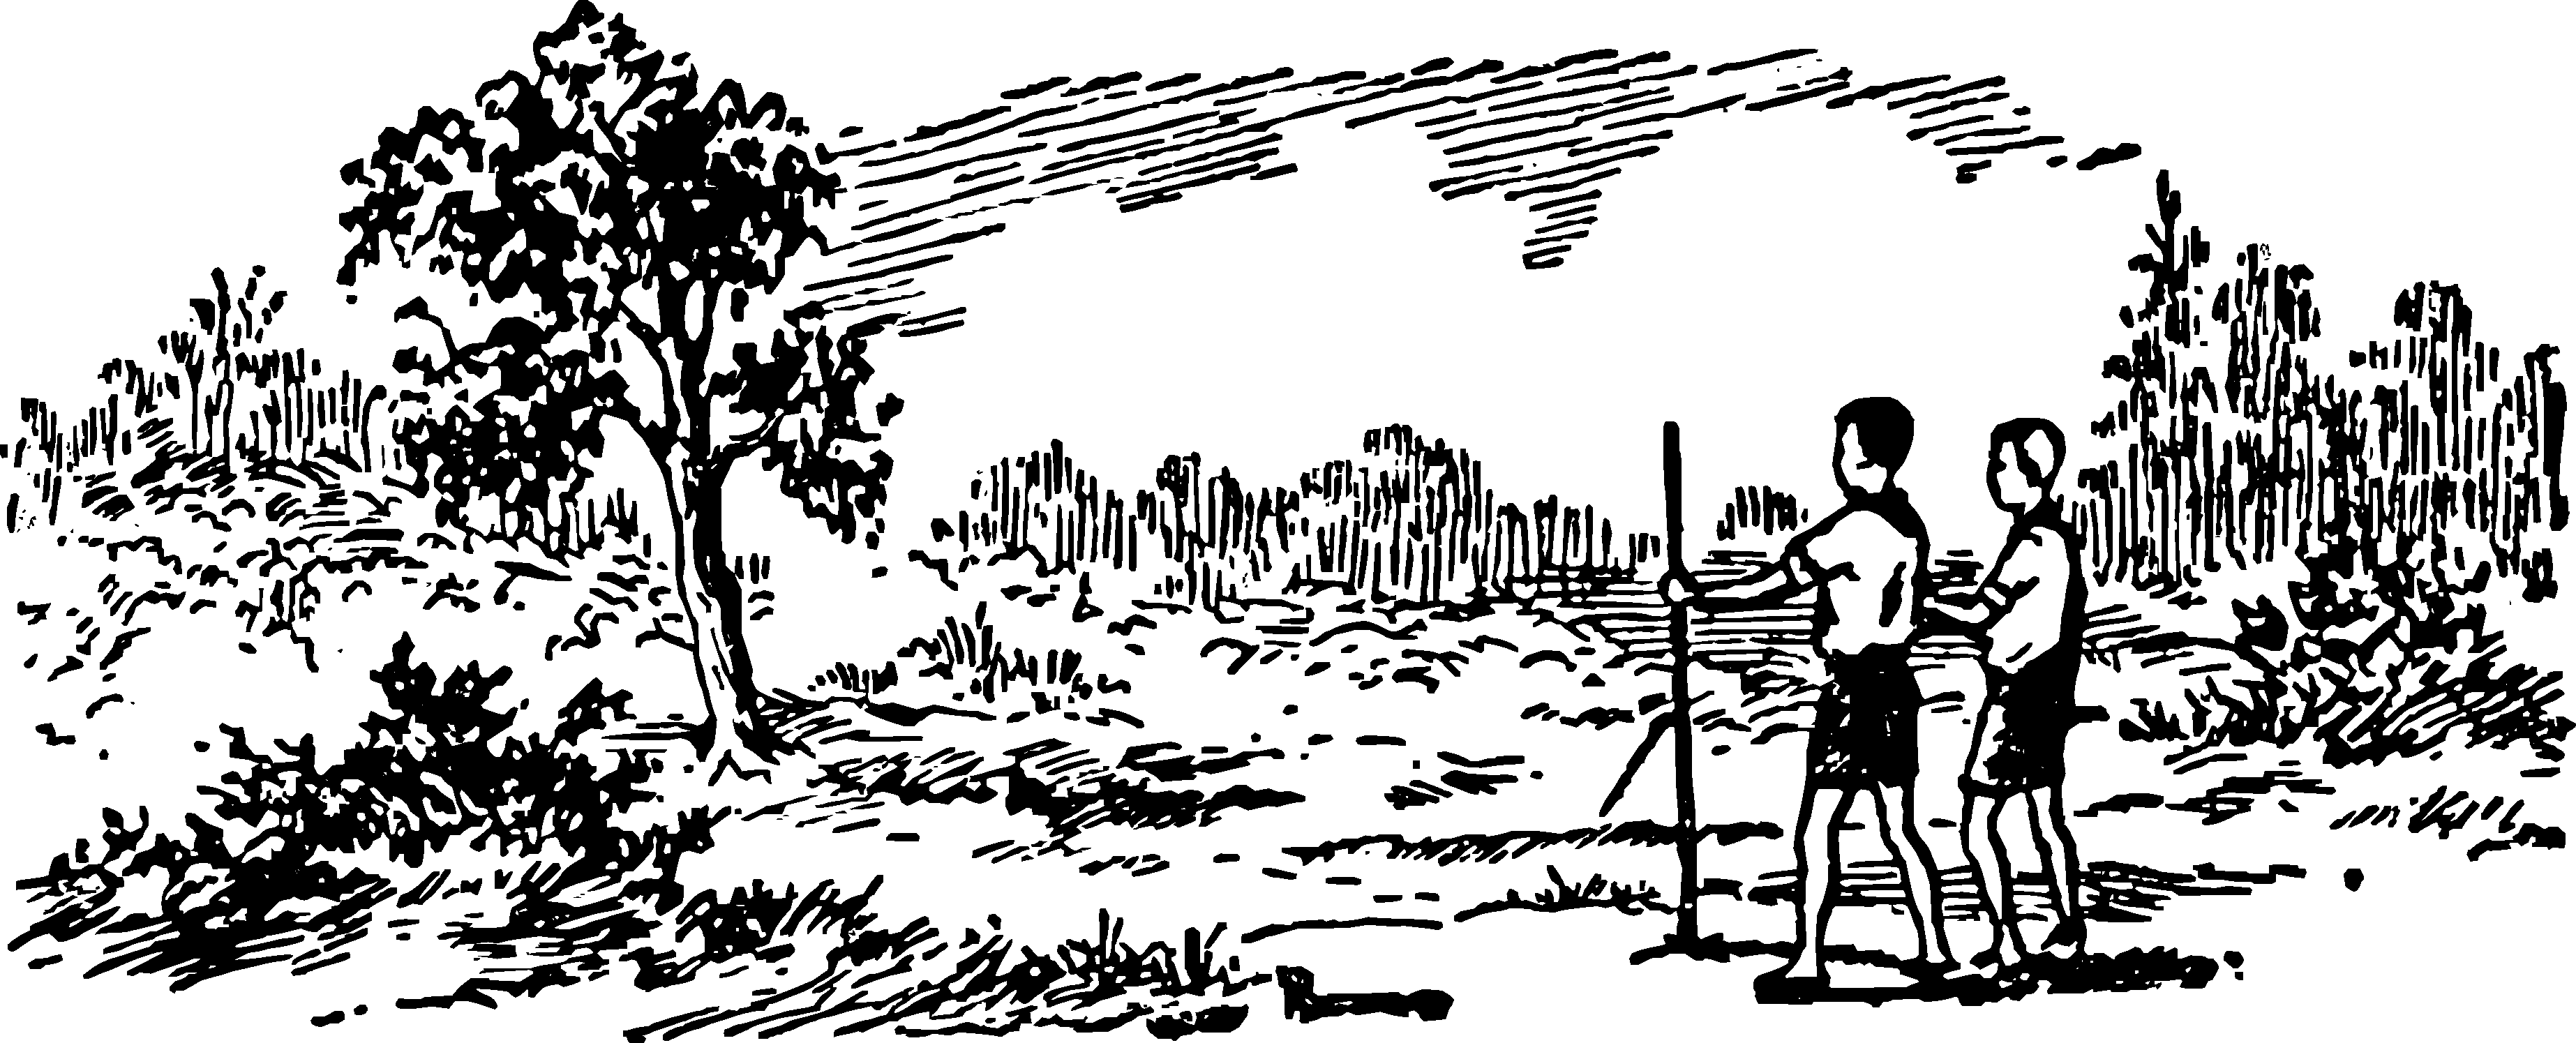
\includegraphics[width=1.2\textwidth]{figures/ch-01/fig-ch-01-head.pdf}\bigskip}

\chapter{Geometry In The Forest}
\label{ch-01}

%\begin{tikzpicture}[remember picture,overlay,shift=(current page.north west)]
%\begin{scope}[x={(current page.north east)},y={(current page.south west)}]
%\node [overlay,remember picture] at (0.5,0.2) {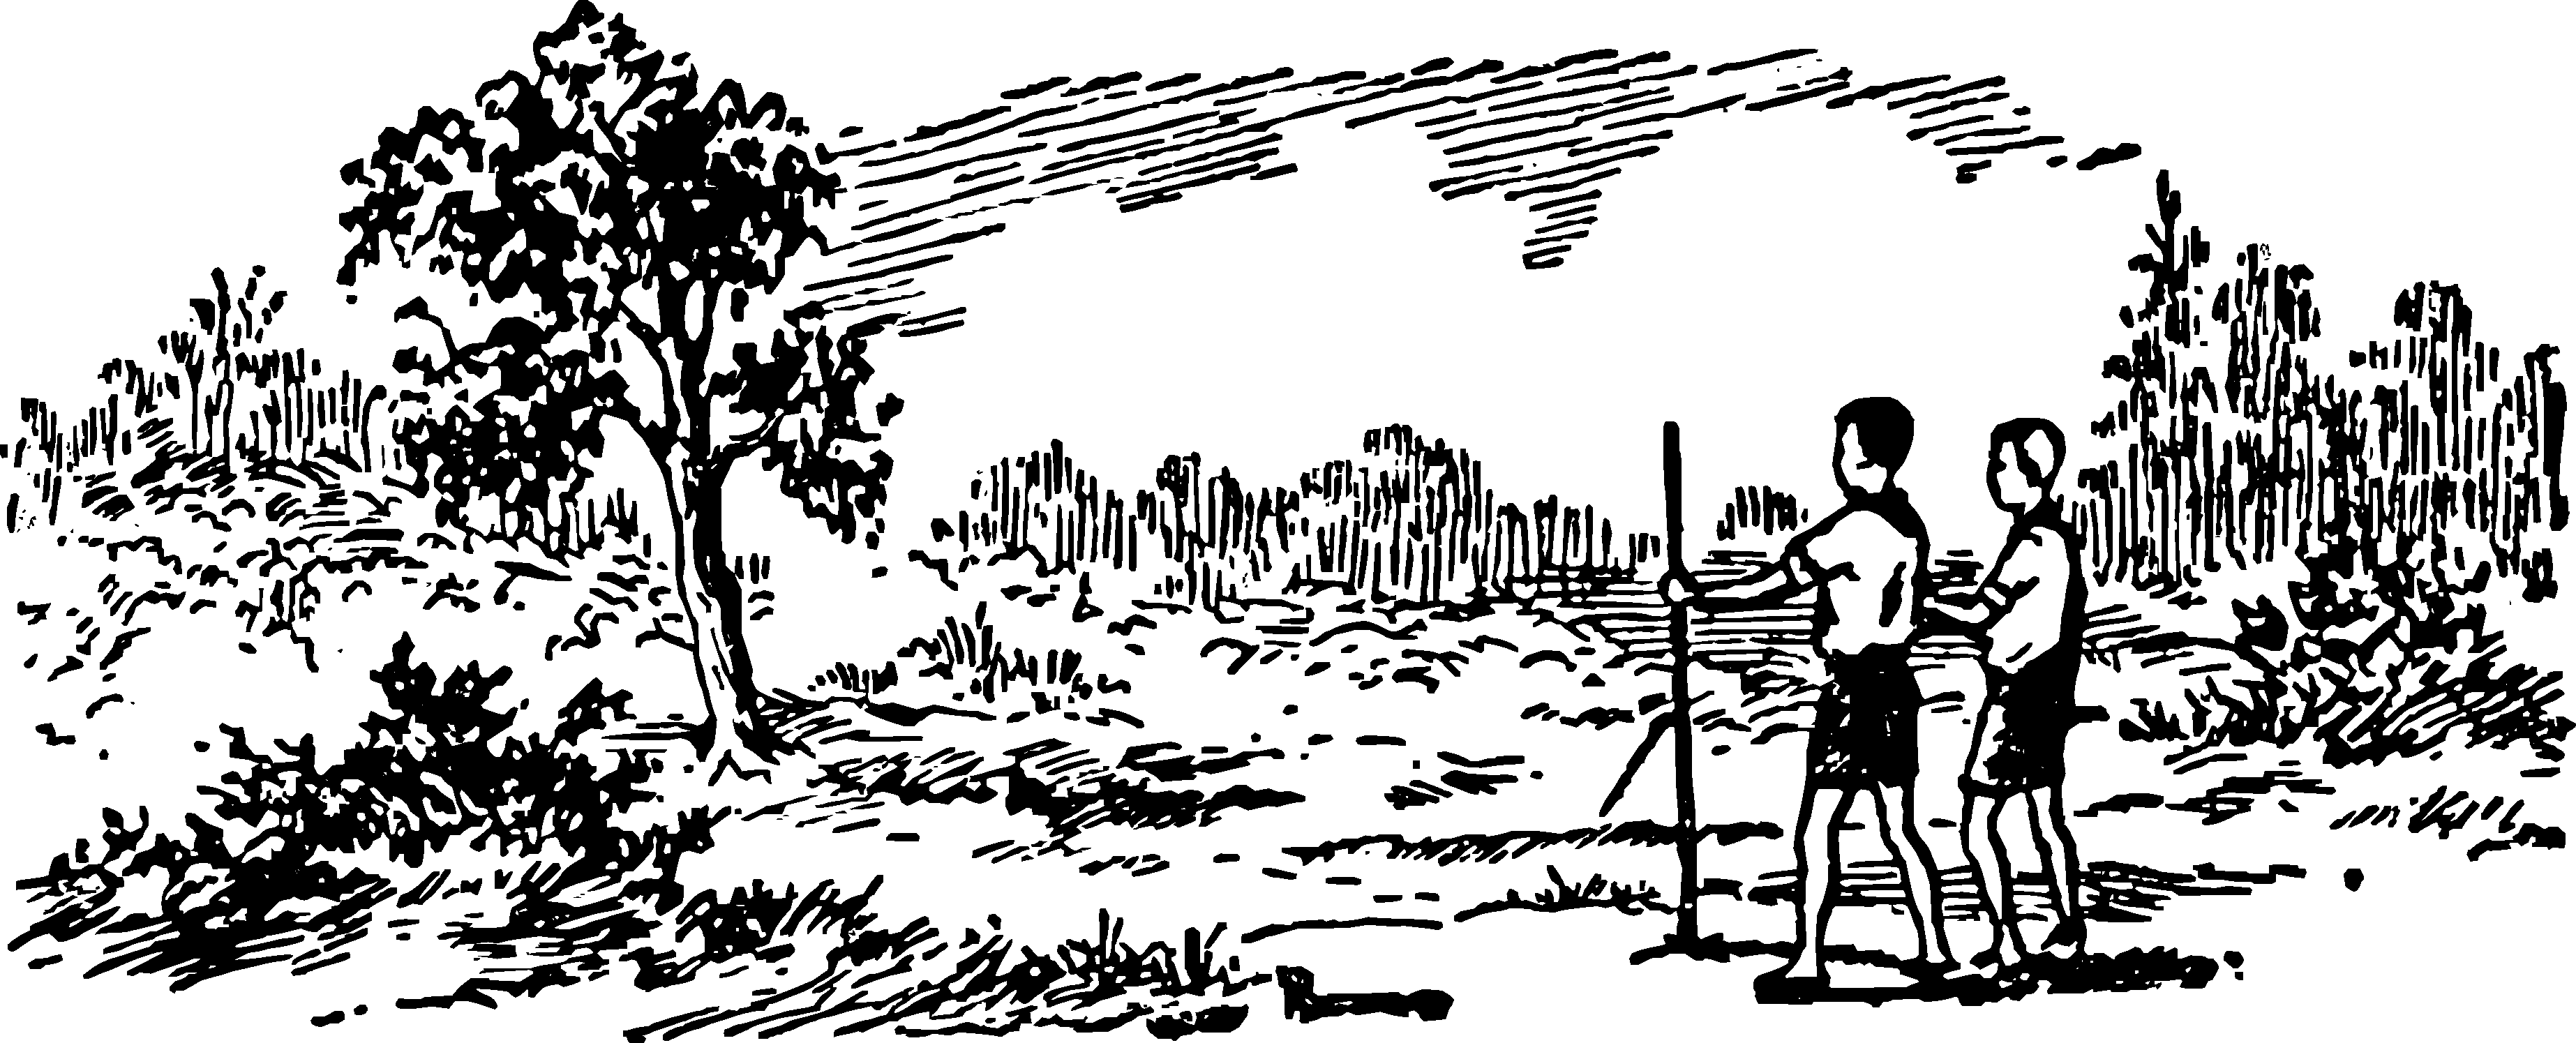
\includegraphics[width=1.2\textwidth]{figures/ch-01/fig-ch-01-head.pdf}};
%\end{scope}
%\end{tikzpicture}

\section{By the length of the shadow}
\label{sec-1.1}

I remember now the amazement with which I looked for the first time, he looked at a gray-haired forester, who, standing near a huge pine tree, measured its height with a small pocket device. When he aimed his square board at the top of the tree, I expected that the old man would now start climbing there with a measuring chain. Instead, he put the device back in his pocket and announced that the measurement was over. I thought it hadn't started yet \ldots{}

I was very young then, and this way of measuring, when a person determines the height of a tree without cutting it down and climbing to the top, was in my eyes something like a small miracle. It was only later, when I was initiated into the rudiments of geometry, that I realised how simple such miracles are performed. There are many different ways to make such measurements using very simple instruments and even without any devices.

The easiest and most ancient way is, without a doubt, the one by which the Greek sage Thales determined the height of the pyramid in Egypt sixth century BC. He took advantage of the pyramid's `shadow'. The priests and the pharaoh, gathered at the foot of the highest pyramid, looked puzzled at the northern newcomer, who guessed the height of the huge structure from the shadow. Thales, says the legend, chose a day and an hour when the length of his own shadow was equal to his height; at this moment, the height of the pyramid should also be equal to the length of the shadow cast by it\sidenote{Of course, the length of the shadow had to be measured from the midpoint of the square base of the pyramid; Thales could directly measure the width of this base.}. This is perhaps the only case when a person benefits from his shadow \ldots{}

The task of the Greek sage now seems childishly simple to us, but let's not forget that we are looking at it from the height of a geometric building erected after Thales. He lived long before Euclid, the author of the wonderful book that taught geometry for two millennia after his death. The truths contained in it, which are now known to every schoolboy, were not yet discovered in the era of Thales. And in order to use the shadow to solve the problem of the height of the pyramid, it was necessary to already know some geometric properties of the triangle, namely the following two (of which Thales himself discovered the first):
\begin{enumerate}
\item that the angles at the base of an isosceles triangle are equal, and vice versa -- that the sides lying opposite the equal angles of the triangle are equal to each other;
\item that the sum of the angles of any triangle (or at least a rectangular one) is equal to two right angles.
\end{enumerate}

Only Thales, armed with this knowledge, had the right to conclude that when his own shadow is equal to his height, the sun's rays meet the flat ground at an angle of half a straight line, and therefore the top of the pyramid, the middle of its base and the end of its shadow should mark an isosceles triangle.

It would seem that this simple method is very convenient to use on a clear sunny day to measure lonely trees whose shadow does not merge with the shadow of neighbouring ones. But in our latitudes it is not as easy as in Egypt to waylay the right moment for this: The sun is low above the horizon, and the shadows are equal to the height of the objects casting them only in the afternoon hours of the summer months. Therefore, the Thales method in this form is not always applicable.

\begin{figure}[h!]
\centering
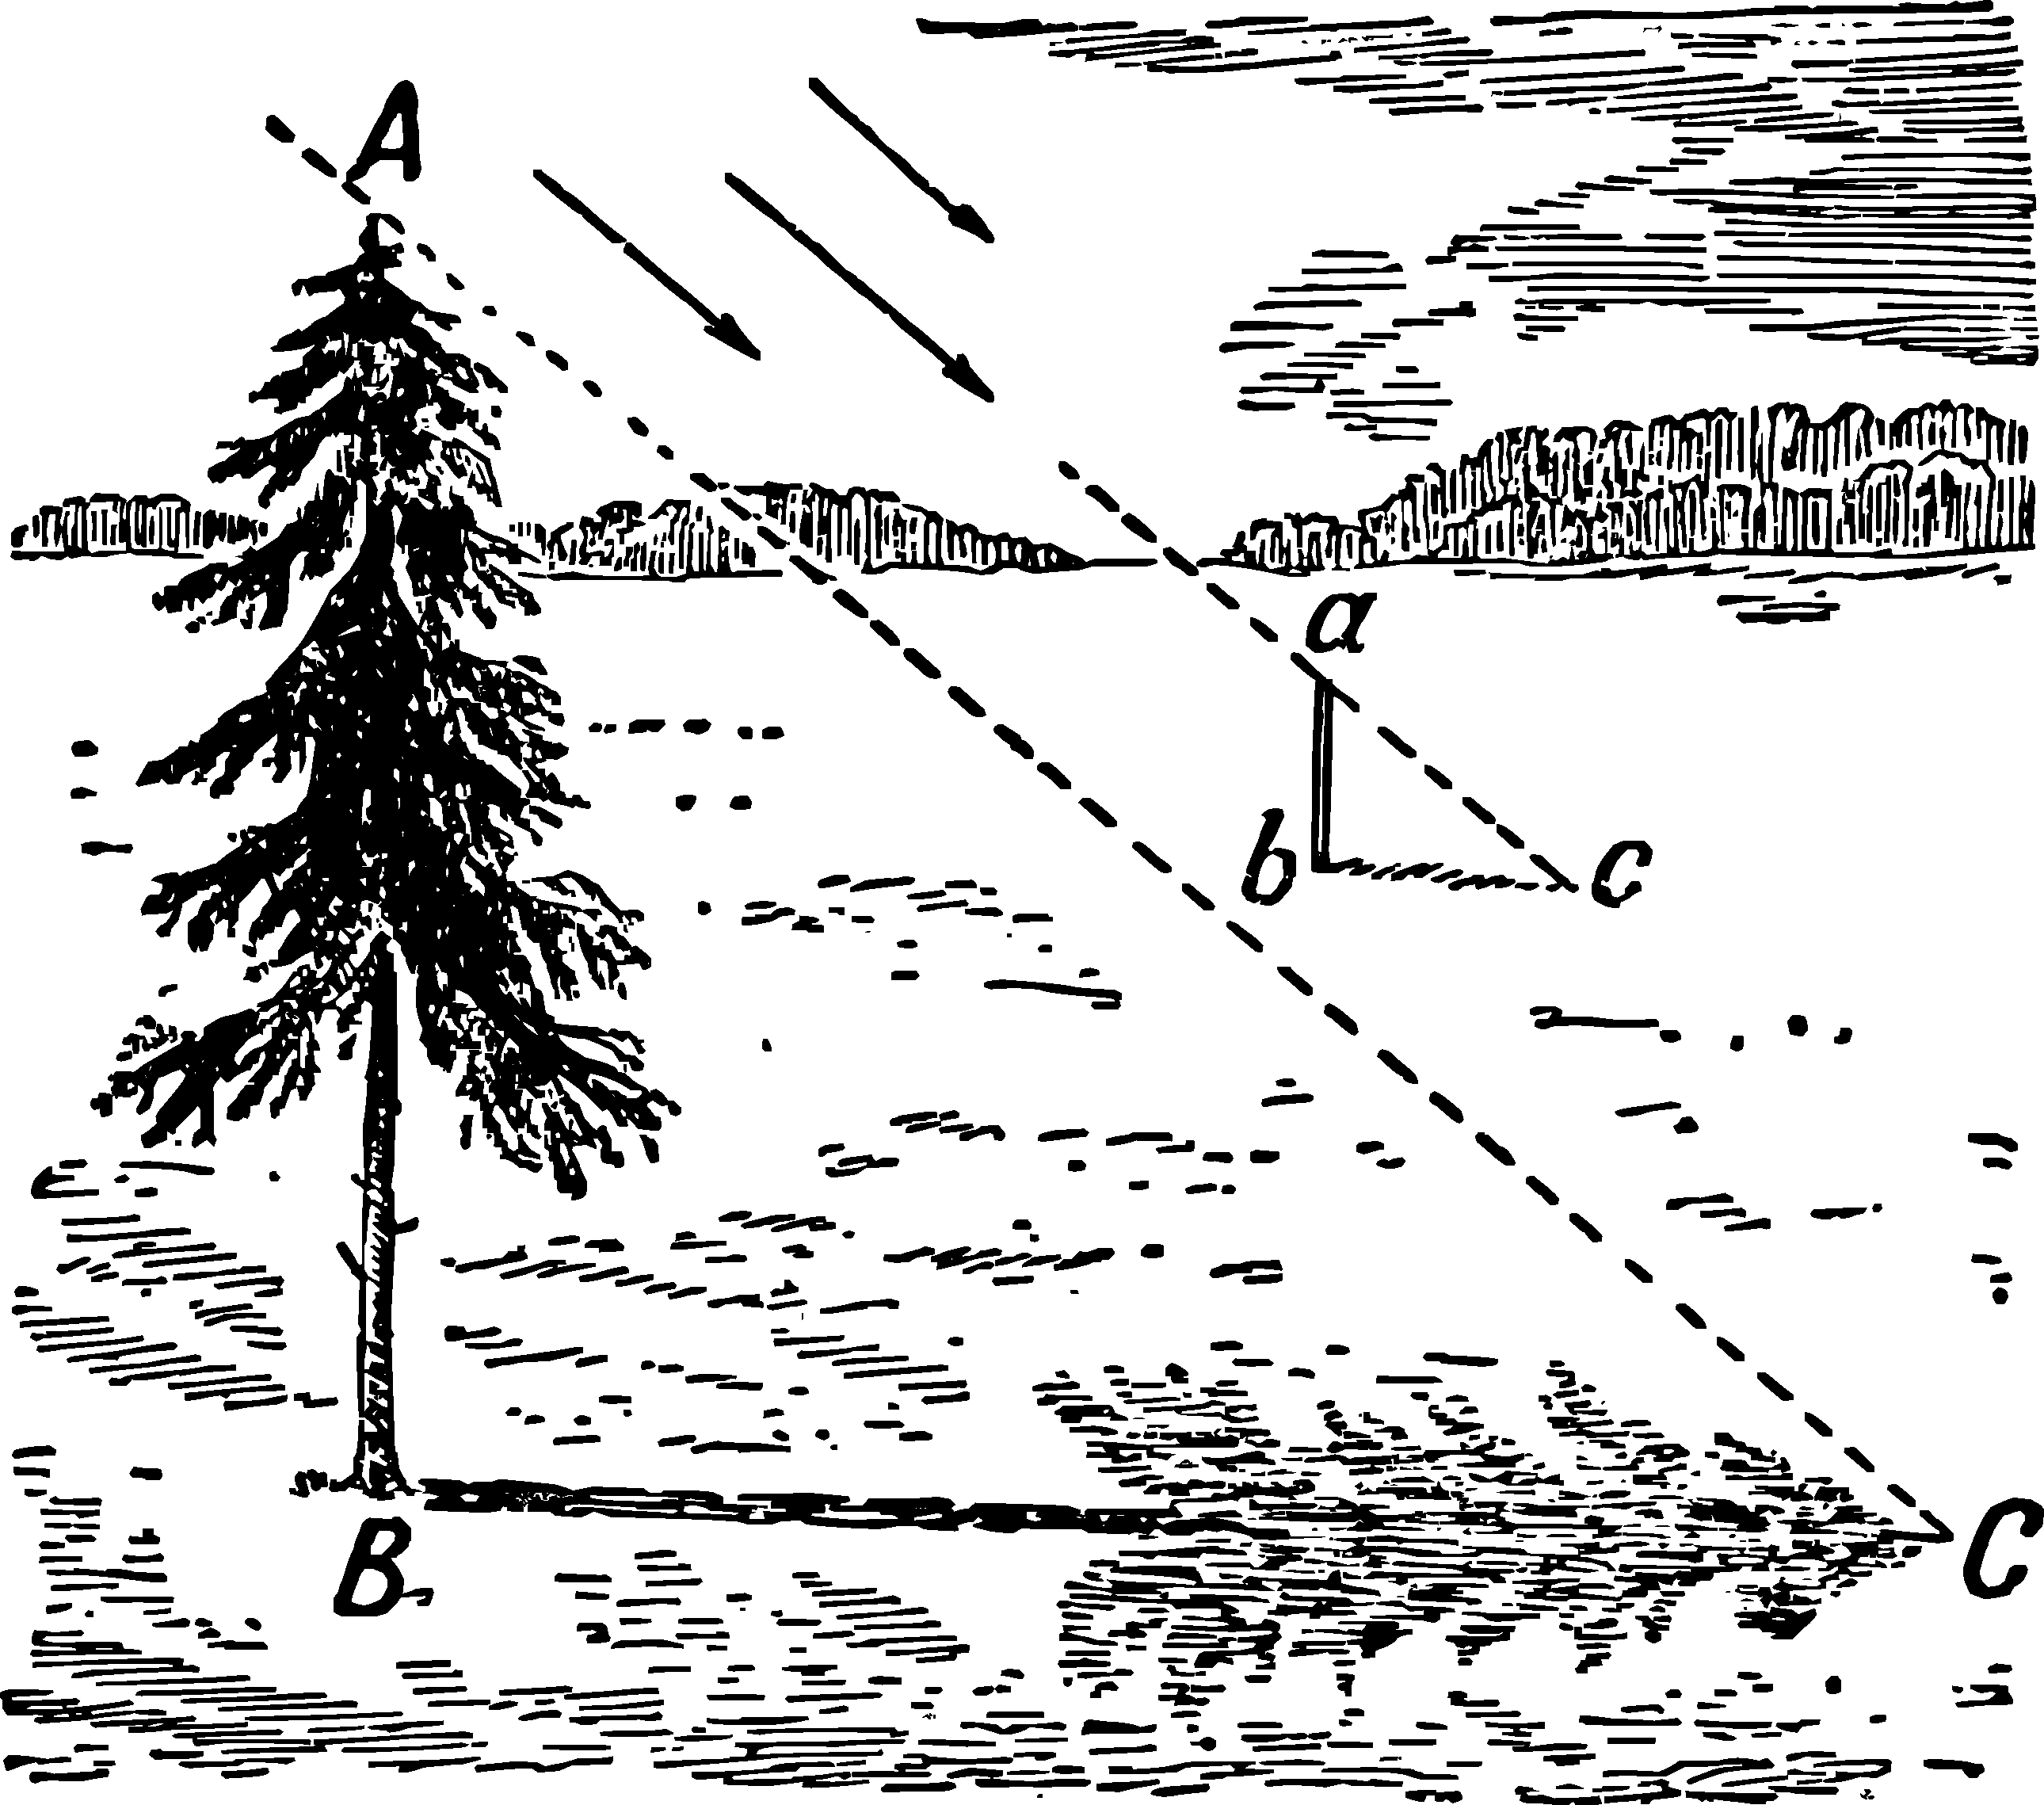
\includegraphics[width=0.9\textwidth]{figures/ch-01/fig-01-01.pdf}
\sidecaption{Measuring the height of a tree by shadow.\label{fig-01-01}}
\end{figure}
It is not difficult, however, to modify this method so that on a sunny day, any shadow can be used, regardless of its length. Additionally, measuring both your own shadow and the shadow of a pole, the desired height is calculated from the proportion (\figr{fig-01-01}):
\begin{equation*}%
AB:ab = BC:bc,
\end{equation*}
meaning the height of the tree is as many times greater than your own height (or the height of the pole) as the shadow of the tree is longer than your shadow (or the shadow of the pole). This naturally follows from the geometric similarity of triangles $ABC$ and $abc$ (based on two angles).

Some readers may object that such an elementary technique does not need a geometric justification at all: is it really unclear even without geometry that how many times is a tree taller, how many times is its shadow longer? However, the matter is not as simple as it seems. Try to apply this rule to shadows cast by the light of a street lamp or lamp -- it will not be justified. In \figr{fig-01-02} you can see that the columns $AB$ are about three times higher than the pedestal $ab$, and the shadow of the column is eight times larger than the shadow of the pedestal $(BC:bc)$. It is impossible to explain why the method is applicable in this case, but not in the other, without geometry.

\begin{figure}[h!]
\centering
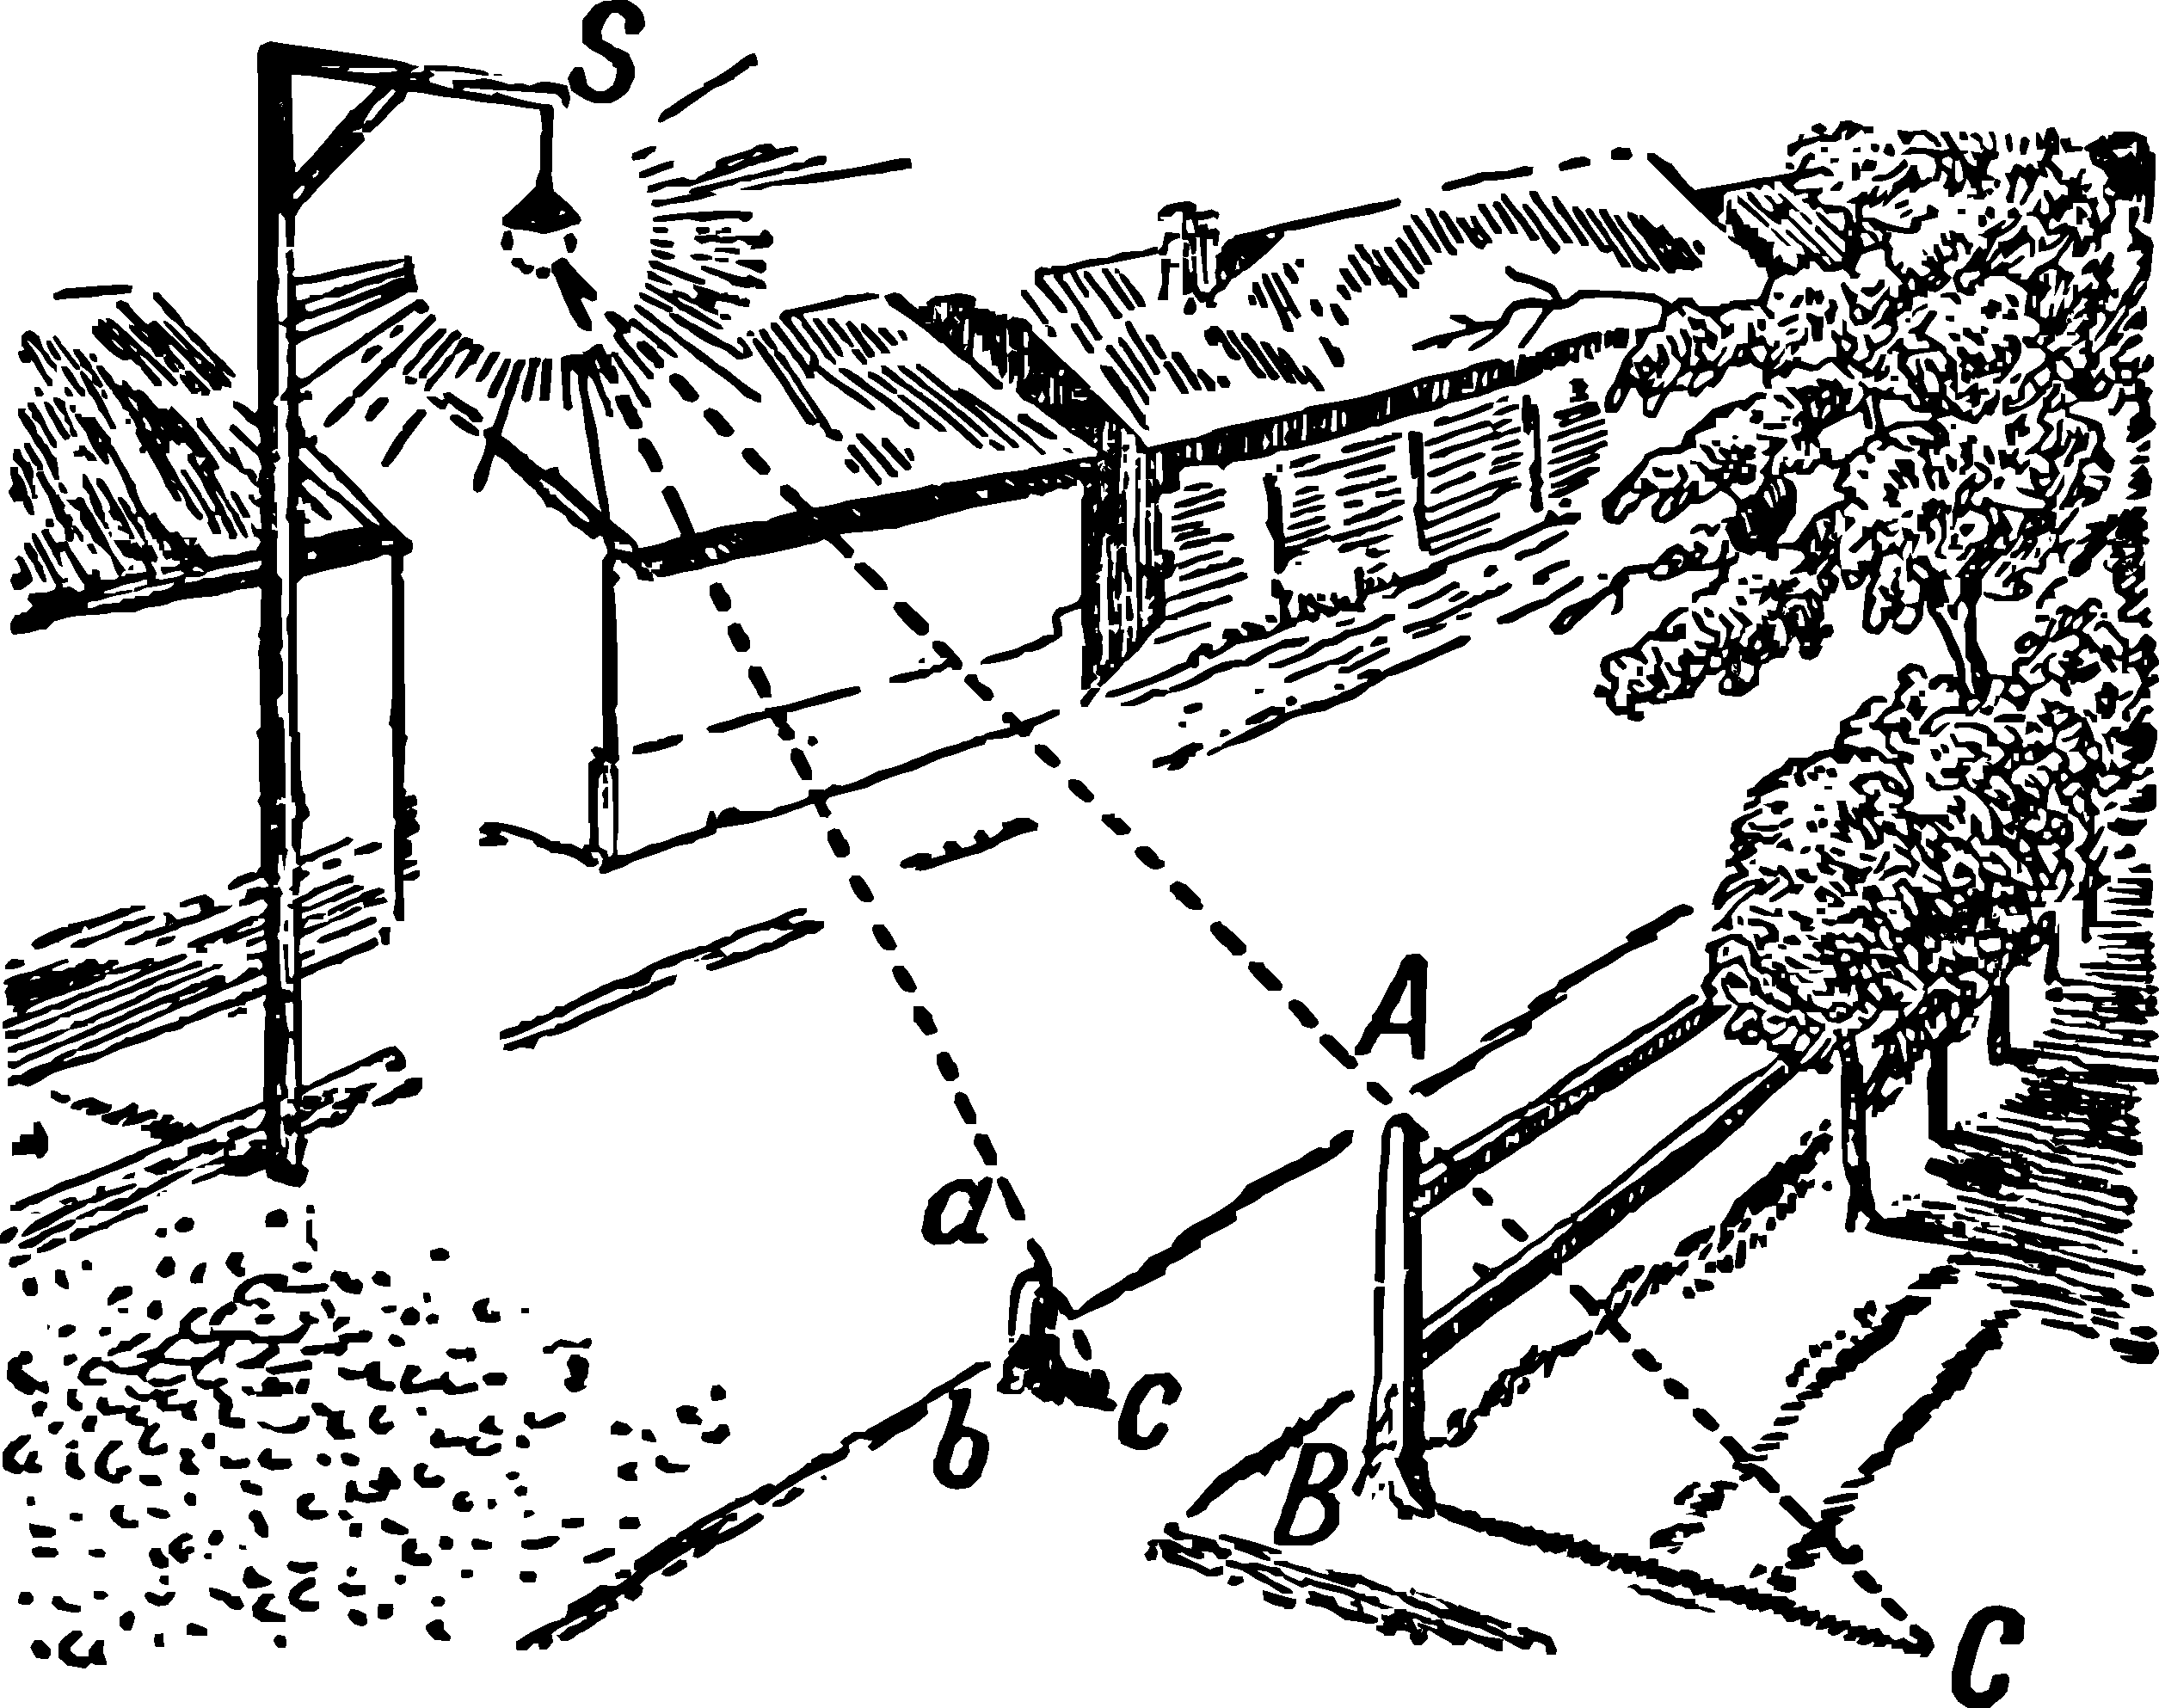
\includegraphics[width=0.9\textwidth]{figures/ch-01/fig-01-02.pdf}
\sidecaption[][0cm]{When such a measurement is impossible. (Is the method applicable for a shadow cast by a streetlamp?)\label{fig-01-02}}
\end{figure}


\ques Let's take a closer look at what the difference is. The essence of the matter boils down. to the fact that the sun's rays are parallel to each other, the rays of the lantern are not parallel. After that, we have the right to consider the rays of the Sun parallel, although they certainly intersect in the place from which they originate.


\ans The rays of the Sun falling on the Earth can be considered parallel because the angle between them is extremely small, almost imperceptible. A simple geometric calculation will convince you of this. Imagine two rays coming from some point of the Sun and falling on the Earth at a distance of, say, one kilo-meter from each other. So, if we put one leg of a compass at this point of the Sun, and with the other we described a circle with a radius equal to the distance from the Sun to the Earth (i.e., with a radius of \SI{150000000}{\kilo\meter}), then an arc of one kilometer in length would appear between our two radii rays. The total length of this gigantic circle would be equal to $2 \pi \times \SI{150000000}{\kilo\meter} = \SI{940000000}{\kilo\meter}$. One degree of it, of course, is 360 times less, i.e. about \SI{2600000}{\kilo\meter}; one arc minute is 60 times less than a degree, i.e. equal to \SI{43000}{\kilo\meter}, and one arc second is another 60 times less, i.e. \SI{720}{\kilo\meter}. But our arc is only \SI{1}{\kilo\meter} in length, so it corresponds to an angle of $1/720 \approx \ang{;;0.00138}$ seconds. This angle is elusive even for the most accurate astronomical instruments; therefore, in practise we can consider the rays of the Sun falling on the Earth as parallel lines.\sidenote{Another thing is the rays directed from some point of the Sun to the ends of the earth's diameter; the angle between them is large enough to measure (about \ang{;;17}); the definition of this angle gave astronomers one of the means to establish how great the distance from the Earth to the Sun is.}

Trying to apply the method of shadows in practise, you will immediately be convinced, however, of its unreliability. Shadows are not delimited so clearly that measuring their length can be done quite accurately. Each shadow cast by the light of the Sun has an indistinctly outlined grey border of penumbra, which gives the border of the shadow uncertainty. This is because the Sun is not a point, but a large luminous body emitting rays from many points. \figr{fig-01-03} illustrates why, as a result of this, the shadow of tree $AB$ also has an additional component in the form of half-shadow $CD$, gradually fading away.

\begin{figure}[h!]
\centering
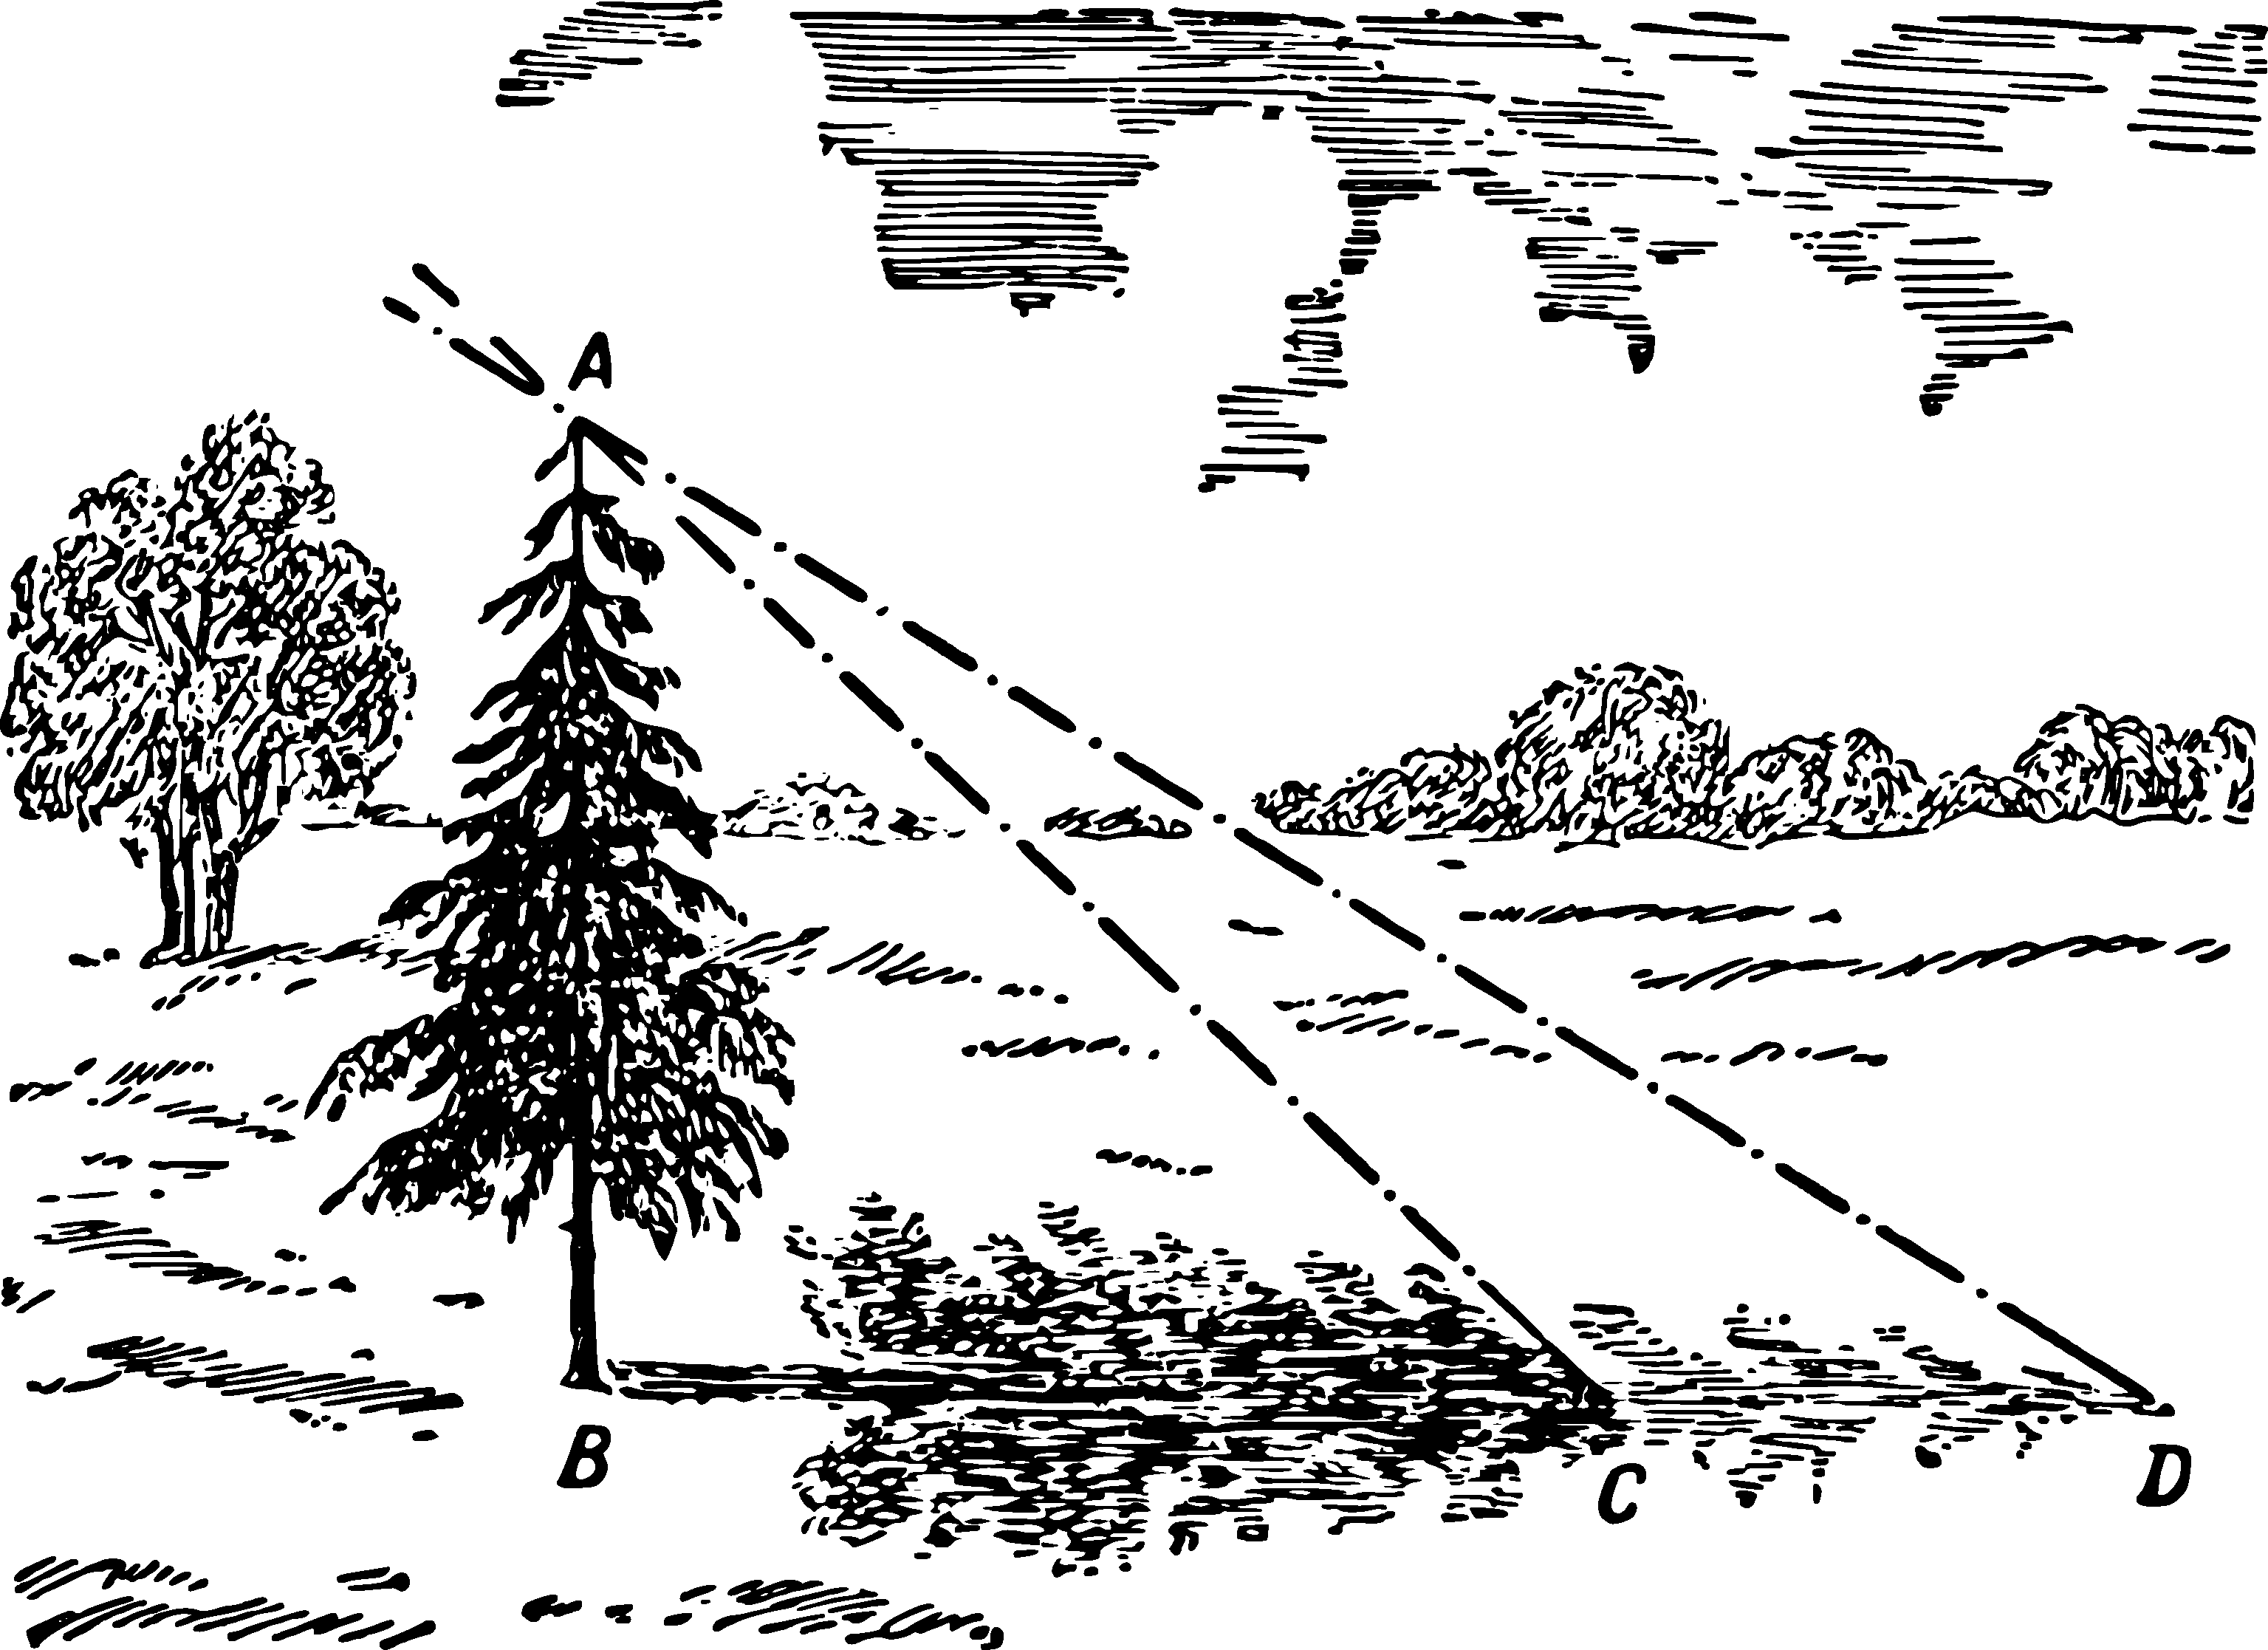
\includegraphics[width=0.9\textwidth]{figures/ch-01/fig-01-03.pdf}
\sidecaption{How penumbra is formed.\label{fig-01-03}}
\end{figure}


The angle of the $CAD$ between the extreme boundaries of the penumbra is equal to the angle at which we always see the solar disk, i.e. half a degree. The error resulting from the fact that both shadows are not measured quite accurately can reach 5\% or more when the Sun is not too low. This error is added to other unavoidable errors -- from uneven soil, etc. -- and makes the final result little reliable. In mountainous terrain, for example, this method is completely inapplicable.

\clearpage

\section{Two More Methods}
\label{sec-1.2}

It is entirely possible to measure height without relying on shadows. There are many methods; let's start with two simple ones.

Firstly, we can utilise the properties of an isosceles right triangle. For this purpose, we can make use of a very simple tool, which can be easily crafted from a piece of board and three pins. On a board of any shape, even a piece of bark with a flat side, mark three points to form the vertices of a right triangle -- and insert a pin at each point (see \figr{fig-01-04}). Suppose you don't have a drafting triangle to construct a right angle, nor a compass to mark equal sides. In that case, fold any piece of paper once, and then fold it again across the first fold so that both parts of the first fold coincide -- and you'll obtain a right angle. The same piece of paper can be used instead of a compass to measure equal distances.

\begin{figure}[h!]
\centering
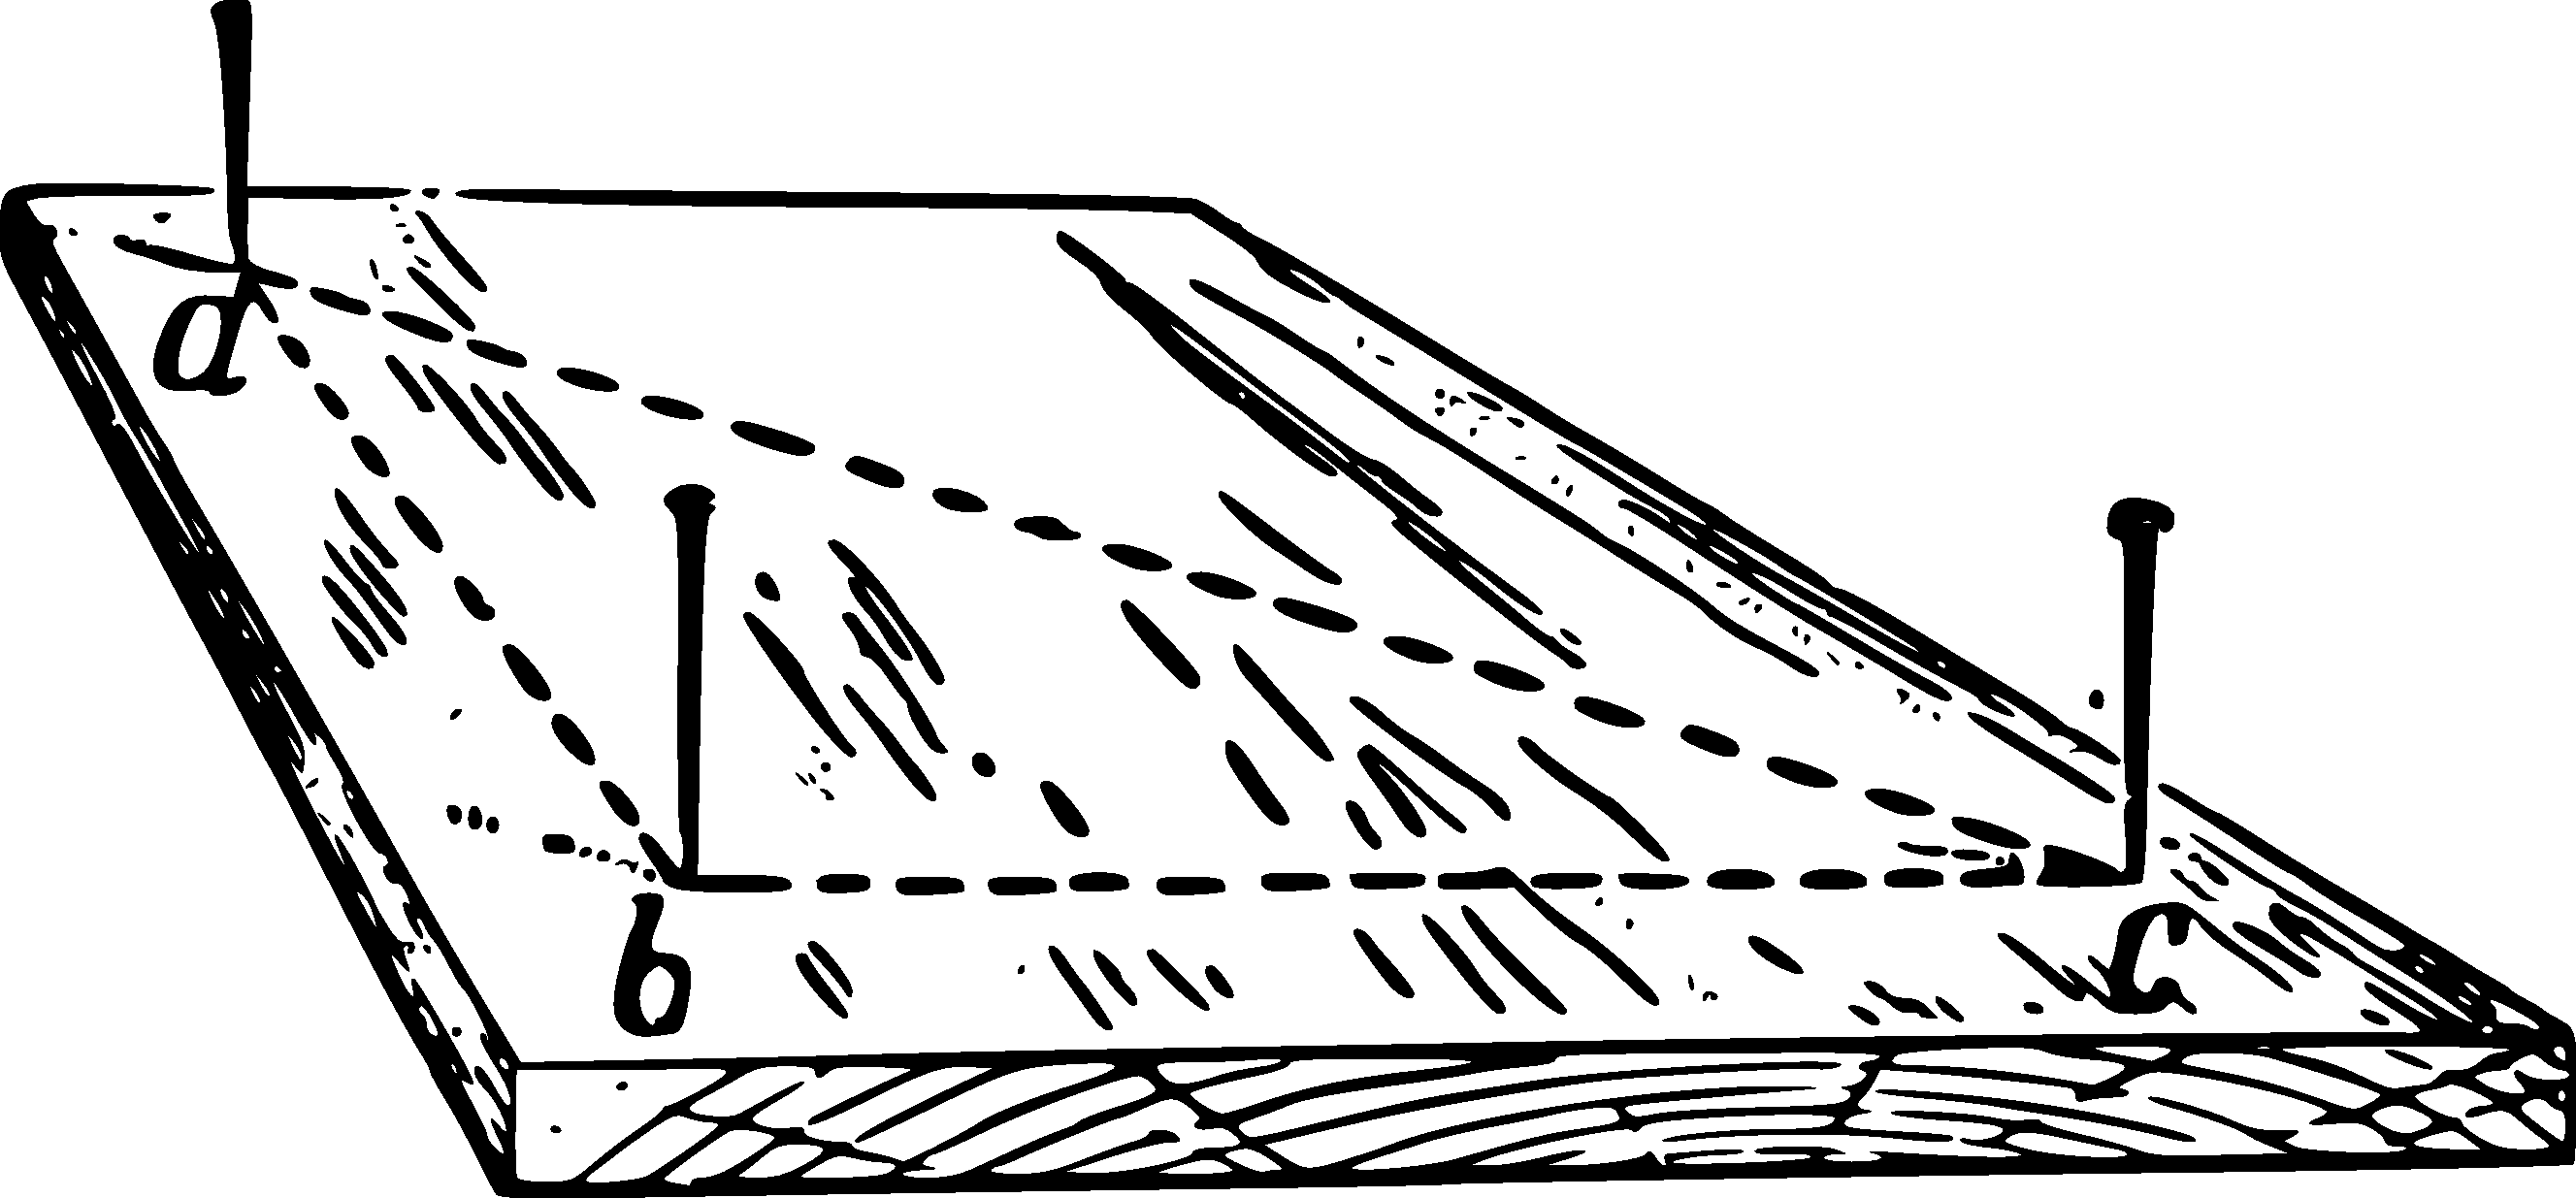
\includegraphics[width=0.6\textwidth]{figures/ch-01/fig-01-04.pdf}
\sidecaption{Pin height measuring device.\label{fig-01-04}}
\end{figure}


As you can see, the tool can be entirely crafted in a makeshift environment.

If you don't have a drafting triangle on hand to construct a right angle, nor a compass to mark equal sides, then simply fold any scrap of paper once, and then fold it again across the first fold so that both parts of the first fold coincide—and you'll obtain a right angle. The same piece of paper can be used instead of a compass to measure equal distances.

As you can see, the tool can be entirely crafted in a makeshift environment.

\begin{figure}[h!]
\centering
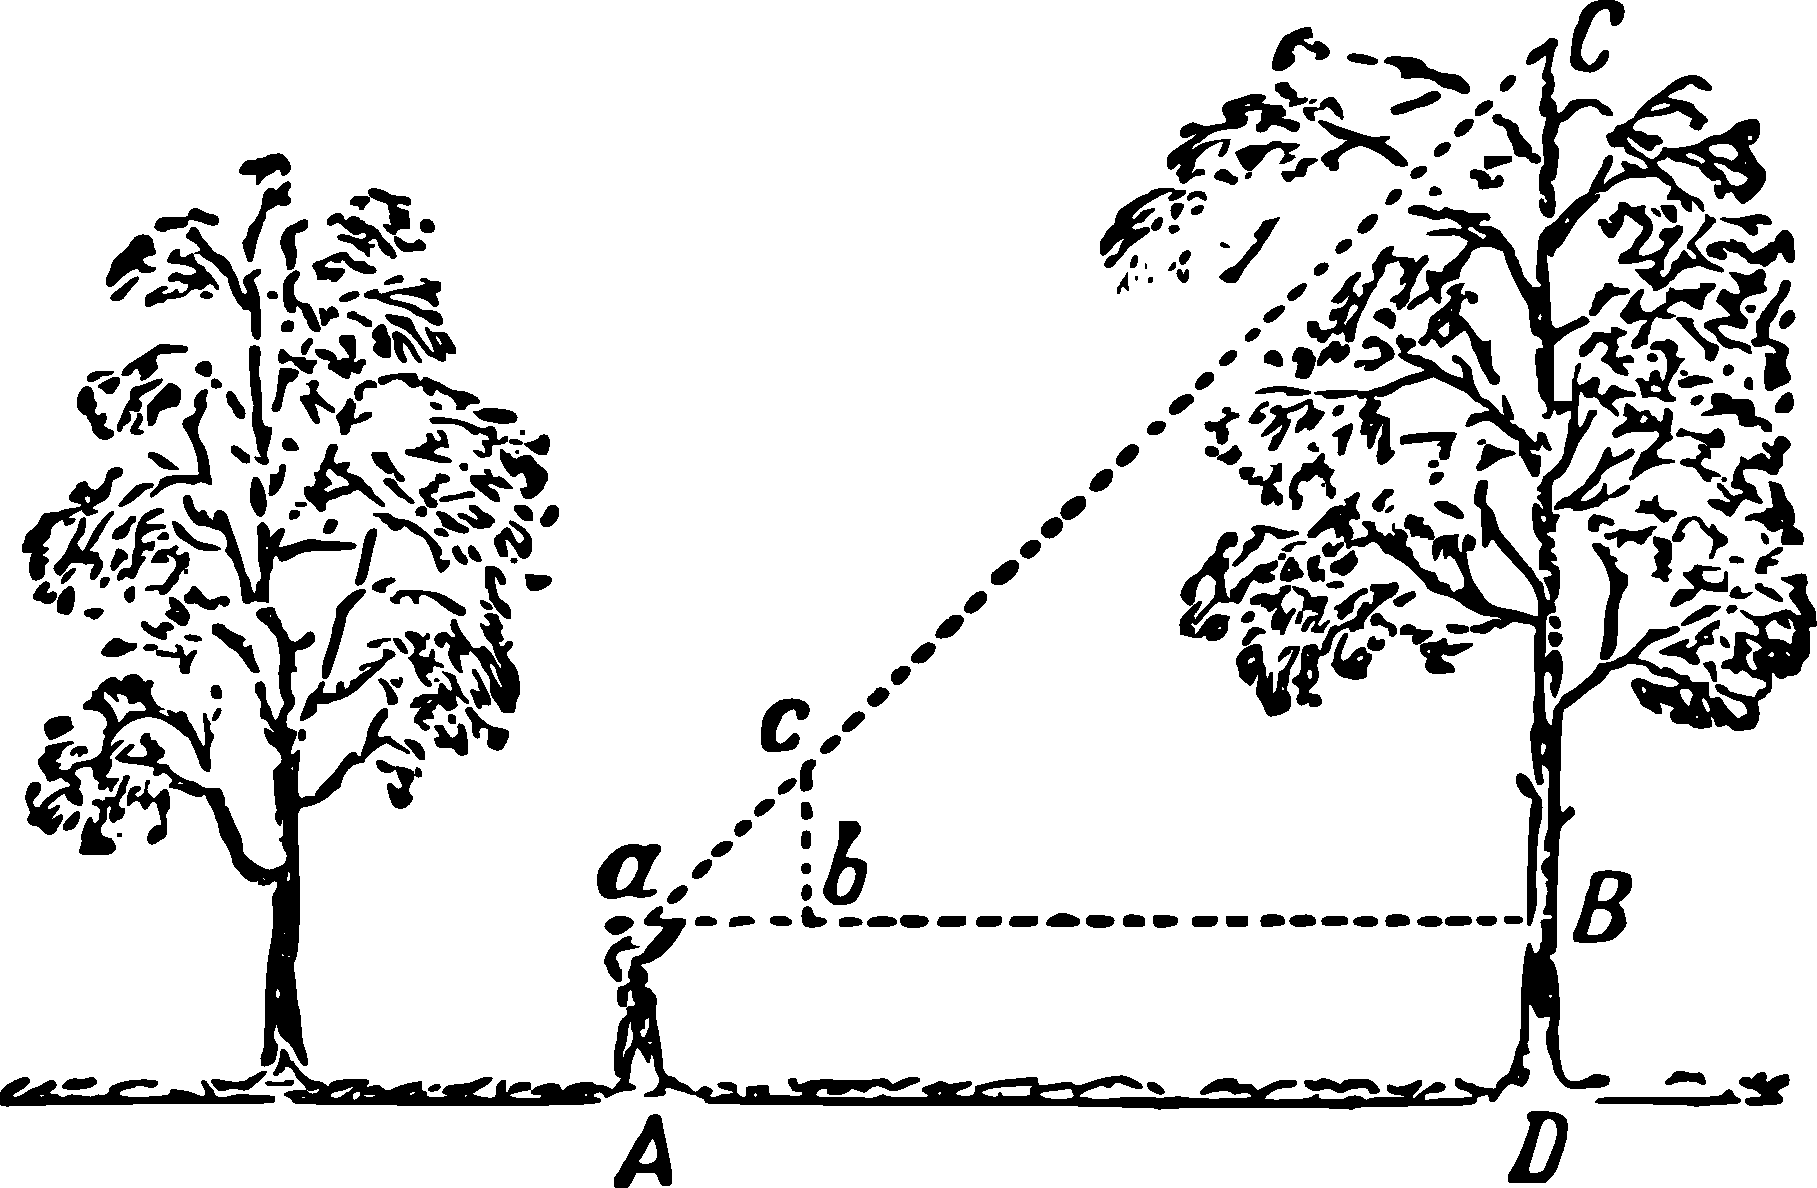
\includegraphics[width=0.9\textwidth]{figures/ch-01/fig-01-05.pdf}
\sidecaption{The scheme of application of the pin device.\label{fig-01-05}}
\end{figure}

Handling it is no more difficult than crafting it. Stepping away from the tree being measured, hold the tool so that one of the legs of the triangle is perpendicular. You can use a string or a weight tied to the top pin. Approaching or moving away from the tree, you will always find a spot $A$ (see \figr{fig-01-05}), from which, looking at pins $a$ and $c$, you will see that they cover the top $C$ of the tree: this means that the extension of the hypotenuse $ac$ passes through point $C$. Then, obviously, the distance $aB$ is equal to $CB$, since angle $a = \ang{45}$. 

Consequently, by measuring distance $aB$ (or, at another location, distance $AD$) and adding $BD$ to it, i.e., the elevation of point $a$ above the ground, you will obtain the desired height of the tree.

\begin{figure}[h!]
\centering
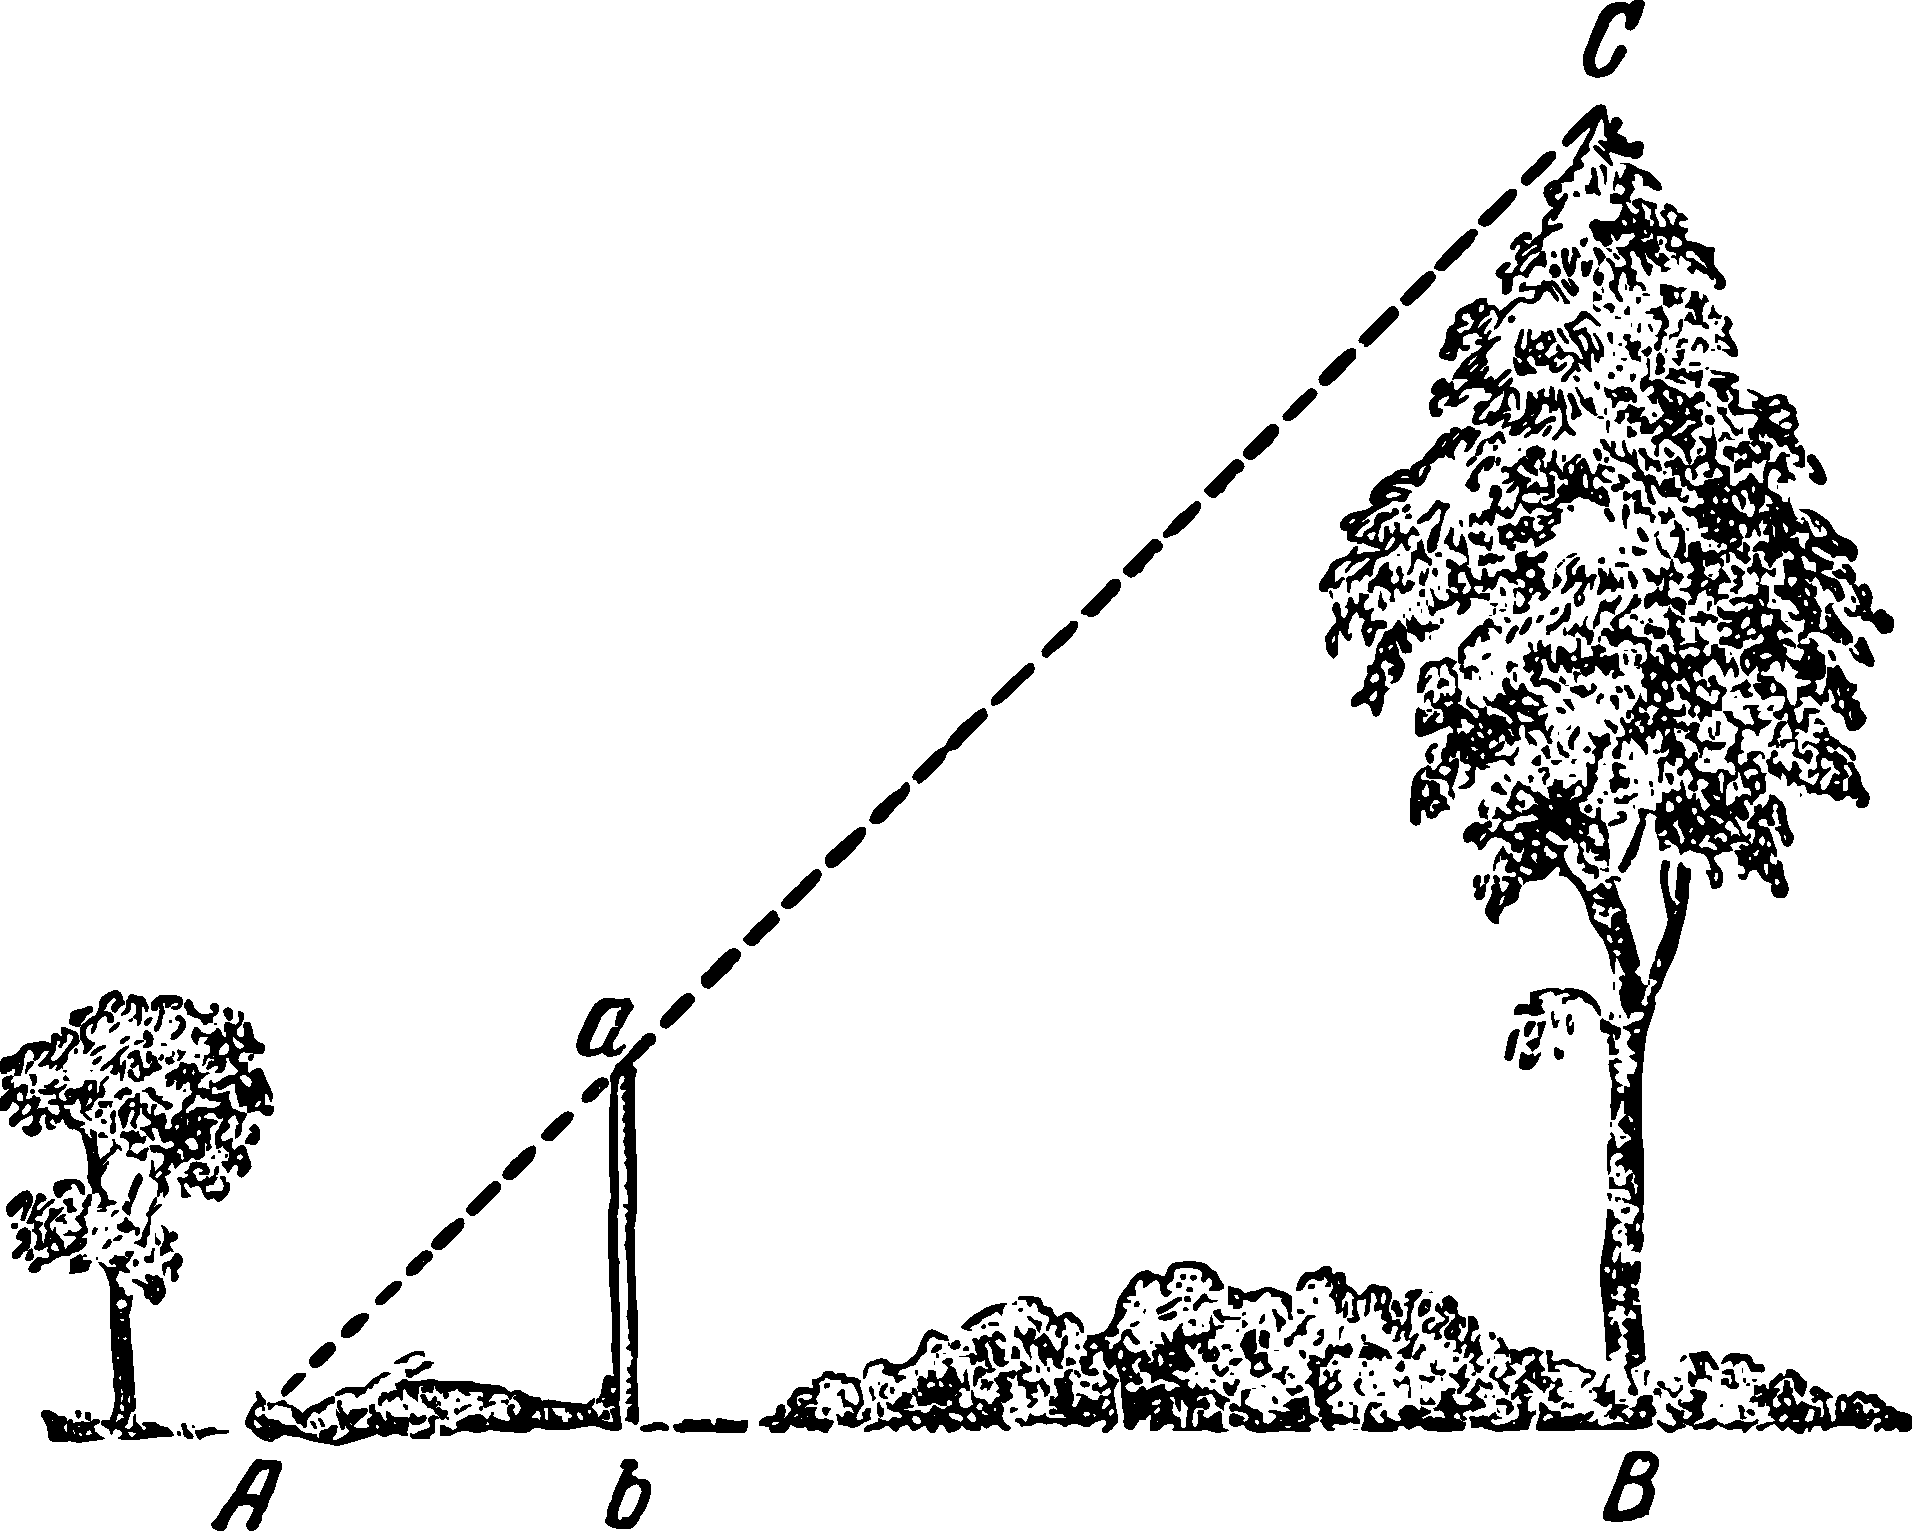
\includegraphics[width=0.9\textwidth]{figures/ch-01/fig-01-06.pdf}
\sidecaption{Another way to determine the height.\label{fig-01-06}}
\end{figure}

Another method does not even require a pin device. Here you need a pole, which you will have to insert vertically into the ground so that the protruding part is exactly at your height. The location for the pole must be chosen so that, lying down as shown in \figr{fig-01-06}, you see the top of the tree in a straight line with the upper point of the pole. Since triangle $Aba$ is isosceles and right-angled, angle $A = \ang{45}$, and therefore $AB$ equals $BC$, i.e., the desired height of the tree.



\section{The Method of Jules Verne}
\label{sec-1.3}

The next, also quite simple, method for measuring tall objects is vividly described by Jules Verne in his famous novel \emph{The Mysterious Island.}

``Today we need to measure the height of the Far View platform,'' said the engineer.

``Will you need a tool for that?'' asked Herbert.

``No, we won't. We'll proceed somewhat differently, resorting to a somewhat simpler and more accurate method.''

The young man, eager to learn as much as possible, followed the engineer, who descended from the granite wall to the rocky shore.

Taking a straight pole, twelve feet long, the engineer measured it as precisely as possible, comparing it to his own height, which he knew well. Meanwhile, Herbert held a plumb bob given to him by the engineer: just a stone attached to the end of a rope.

Not reaching five hundred feet from the granite wall, which rose vertically, the engineer drove the pole two feet into the sand and firmly secured it, placing it vertically with the help of the plumb bob.

\begin{figure}[h!]
\centering
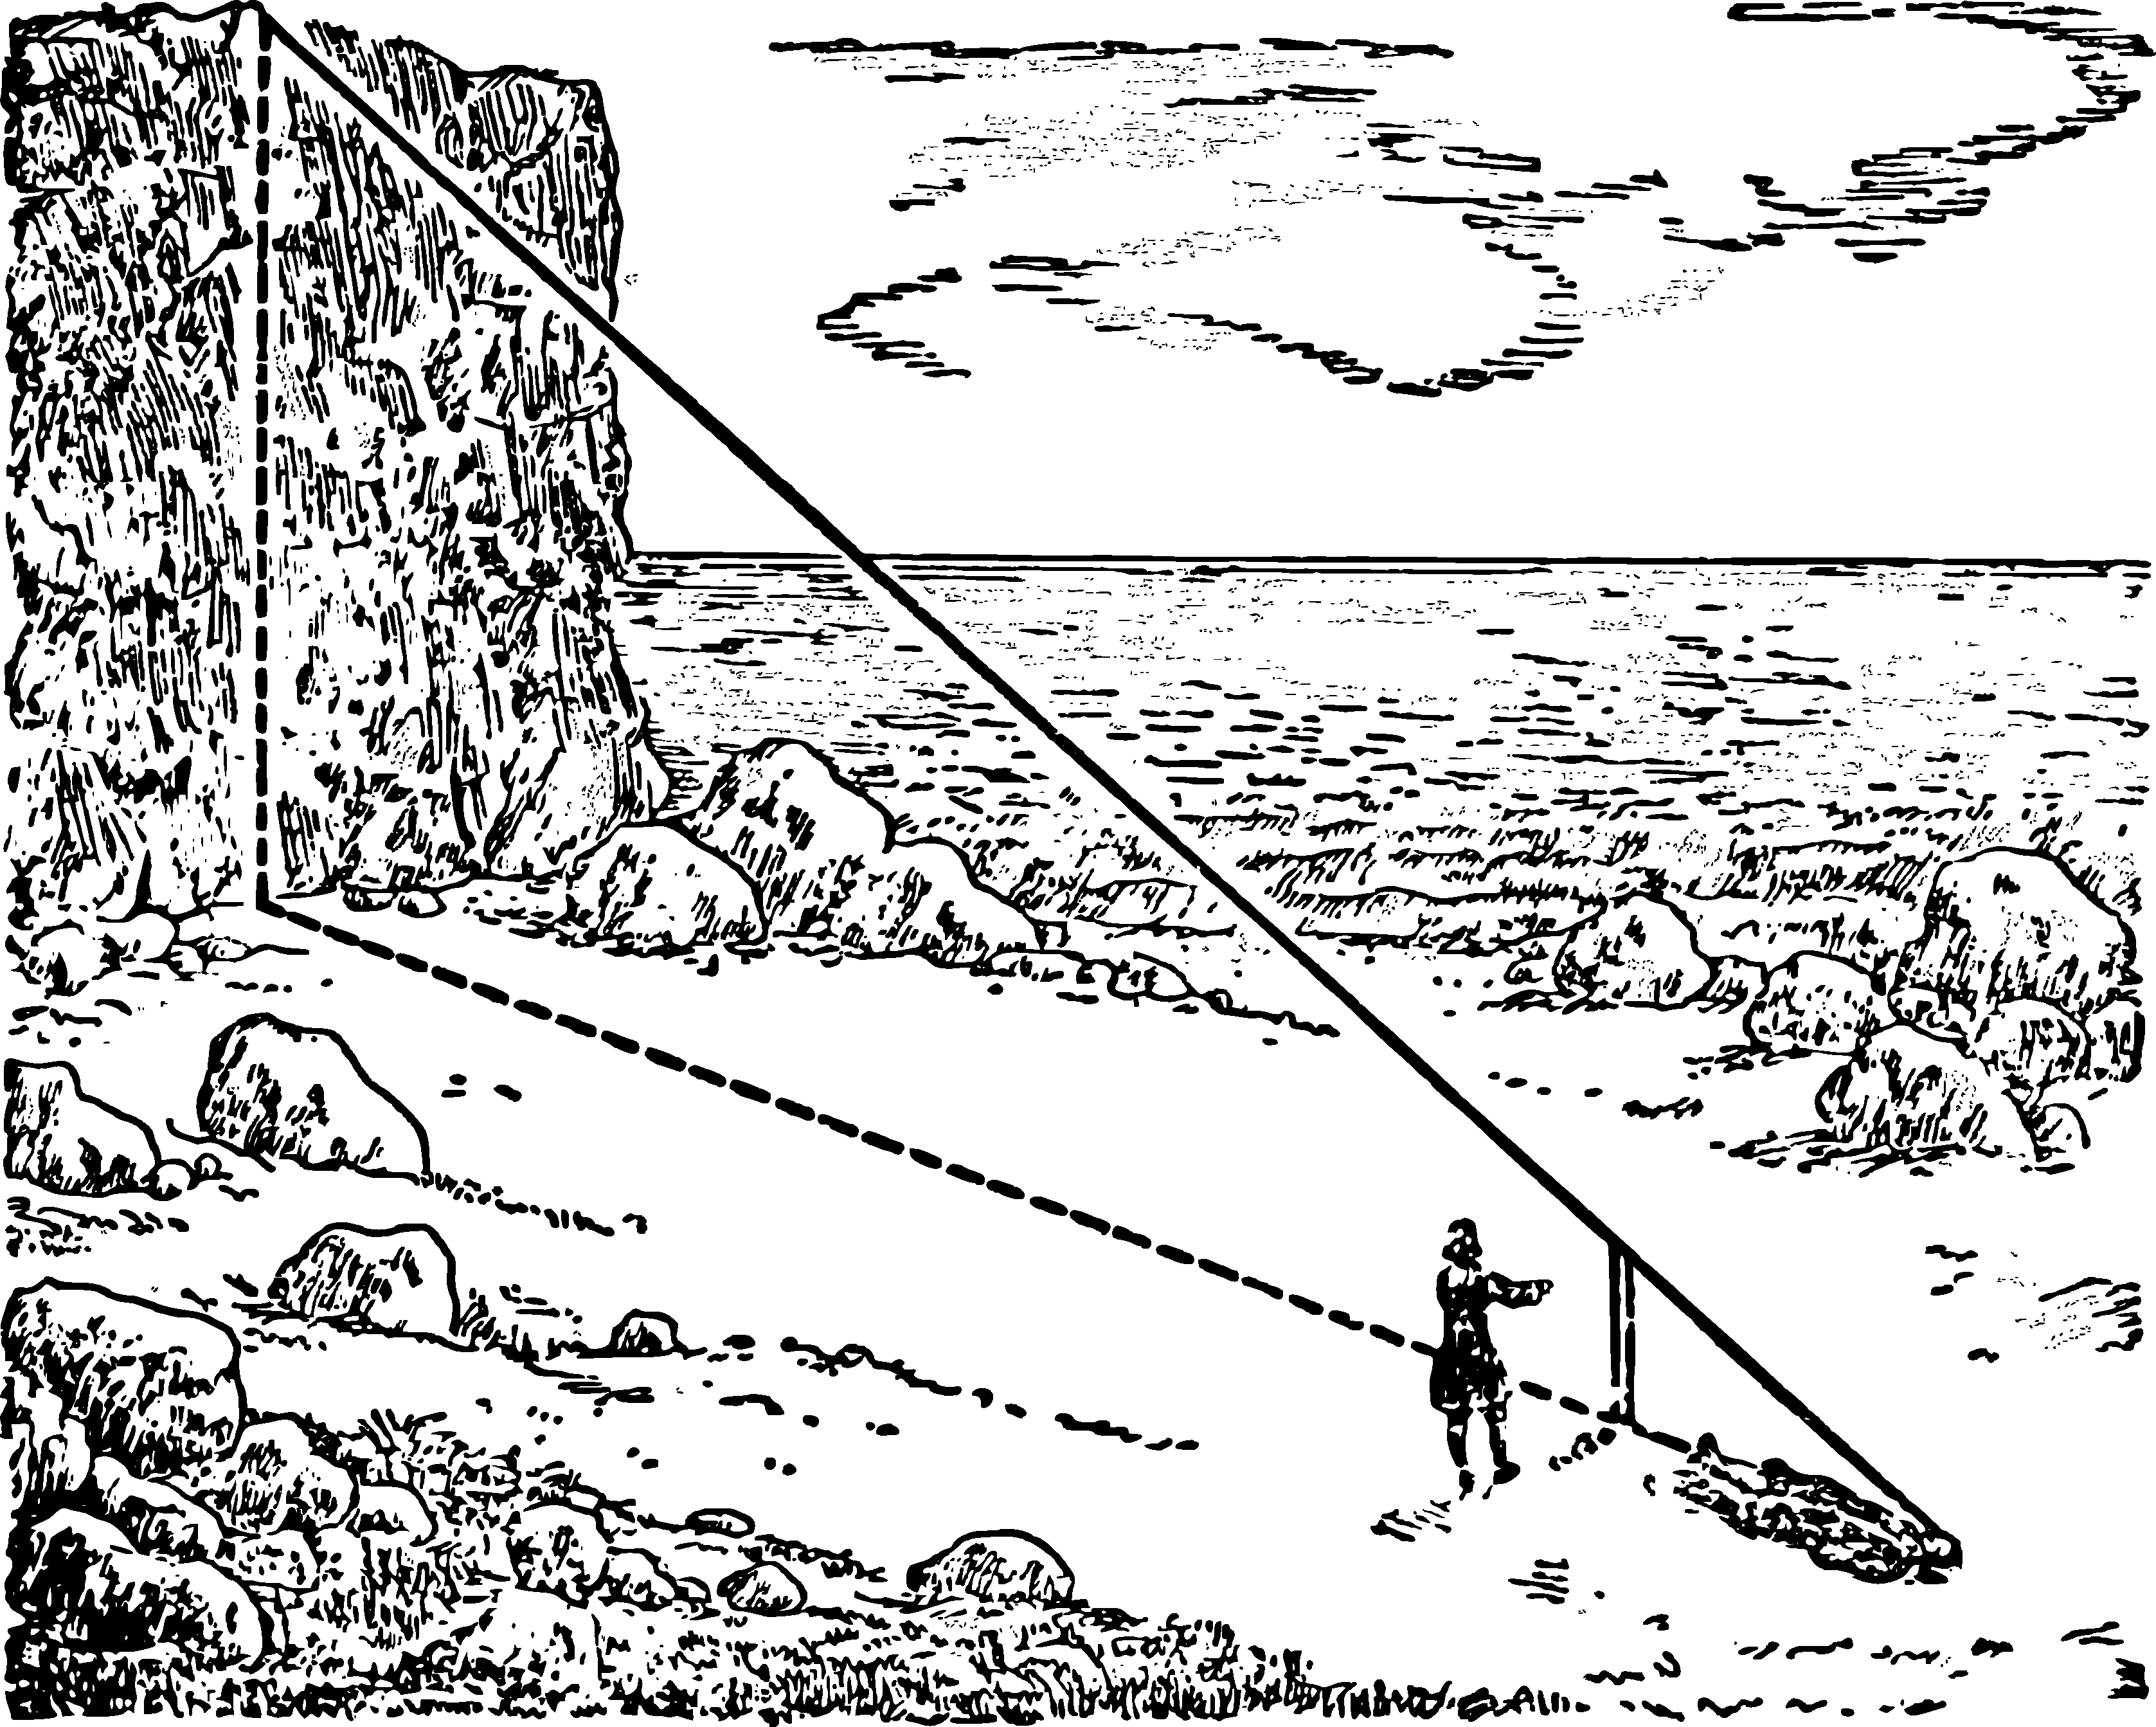
\includegraphics[width=0.9\textwidth]{figures/ch-01/fig-01-07.pdf}
\sidecaption{How the heroes of Jules Verne measured the height of the cliff.\label{fig-01-07}}
\end{figure}

Then he moved away from the pole to a distance where, lying on the sand, one could see both the end of the pole and the edge of the ridge in a straight line (see \figr{fig-01-07}). He carefully marked this point with a stake.

``Are you familiar with the basics of geometry?'' he asked Herbert as he rose from the ground.

``Yes.''

``Do you remember the properties of similar triangles?''

``Their corresponding sides are proportional.''

``Exactly. So now I'll construct two similar right triangles. In the smaller one, one leg will be the plumb-line pole, and the other will be the distance from the stake to the base of the pole; the hypotenuse will be my line of sight. In the other triangle, the legs will be: the granite wall, the height of which we want to determine, and the distance from the stake to the base of this wall; the hypotenuse will be my line of sight, coinciding with the direction of the hypotenuse of the first triangle.''

``Understood!'' exclaimed the youth. ``The distance from the stake to the pole is related to the distance from the stake to the base of the wall, as the height of the pole is to the height of the wall.''

``Yes. And consequently, if we measure the first two distances, then, knowing the height of the pole, we can calculate the fourth, unknown term of the proportion, i.e., the height of the wall. In this way, we can manage without directly measuring the height.''

Both horizontal distances were measured: the smaller one was 15 feet, the larger one was 500 feet.

At the end of the measurements, the engineer made the following record:
\begin{align*}%
15 : 500 & = 10 : x,\\
500 \times 10 & = 5000,\\
5000 : 15 & = 333.3.
\end{align*}
Thus, the height of the granite wall was 333 feet.


\section{How Sergeant Popov Acted}
\label{sec-1.4}

Some of the methods described for measuring height are inconvenient as they require lying on the ground. This inconvenience can, of course, be avoided.

Here's a story from one of the fronts of the Great Patriotic War. Lieutenant Ivanyuk's unit was ordered to build a bridge across a mountain river. On the opposite bank were entrenched fascists. To scout the location for the bridge, the lieutenant assigned a reconnaissance group led by Senior Sergeant Popov. In the nearest forest, they measured the diameter and height of the most typical trees and counted the number of trees that could be used for construction.

They measured the height of the trees using a pole (stick) as shown in \figr{fig-01-08}.

\begin{figure}[h!]
\centering
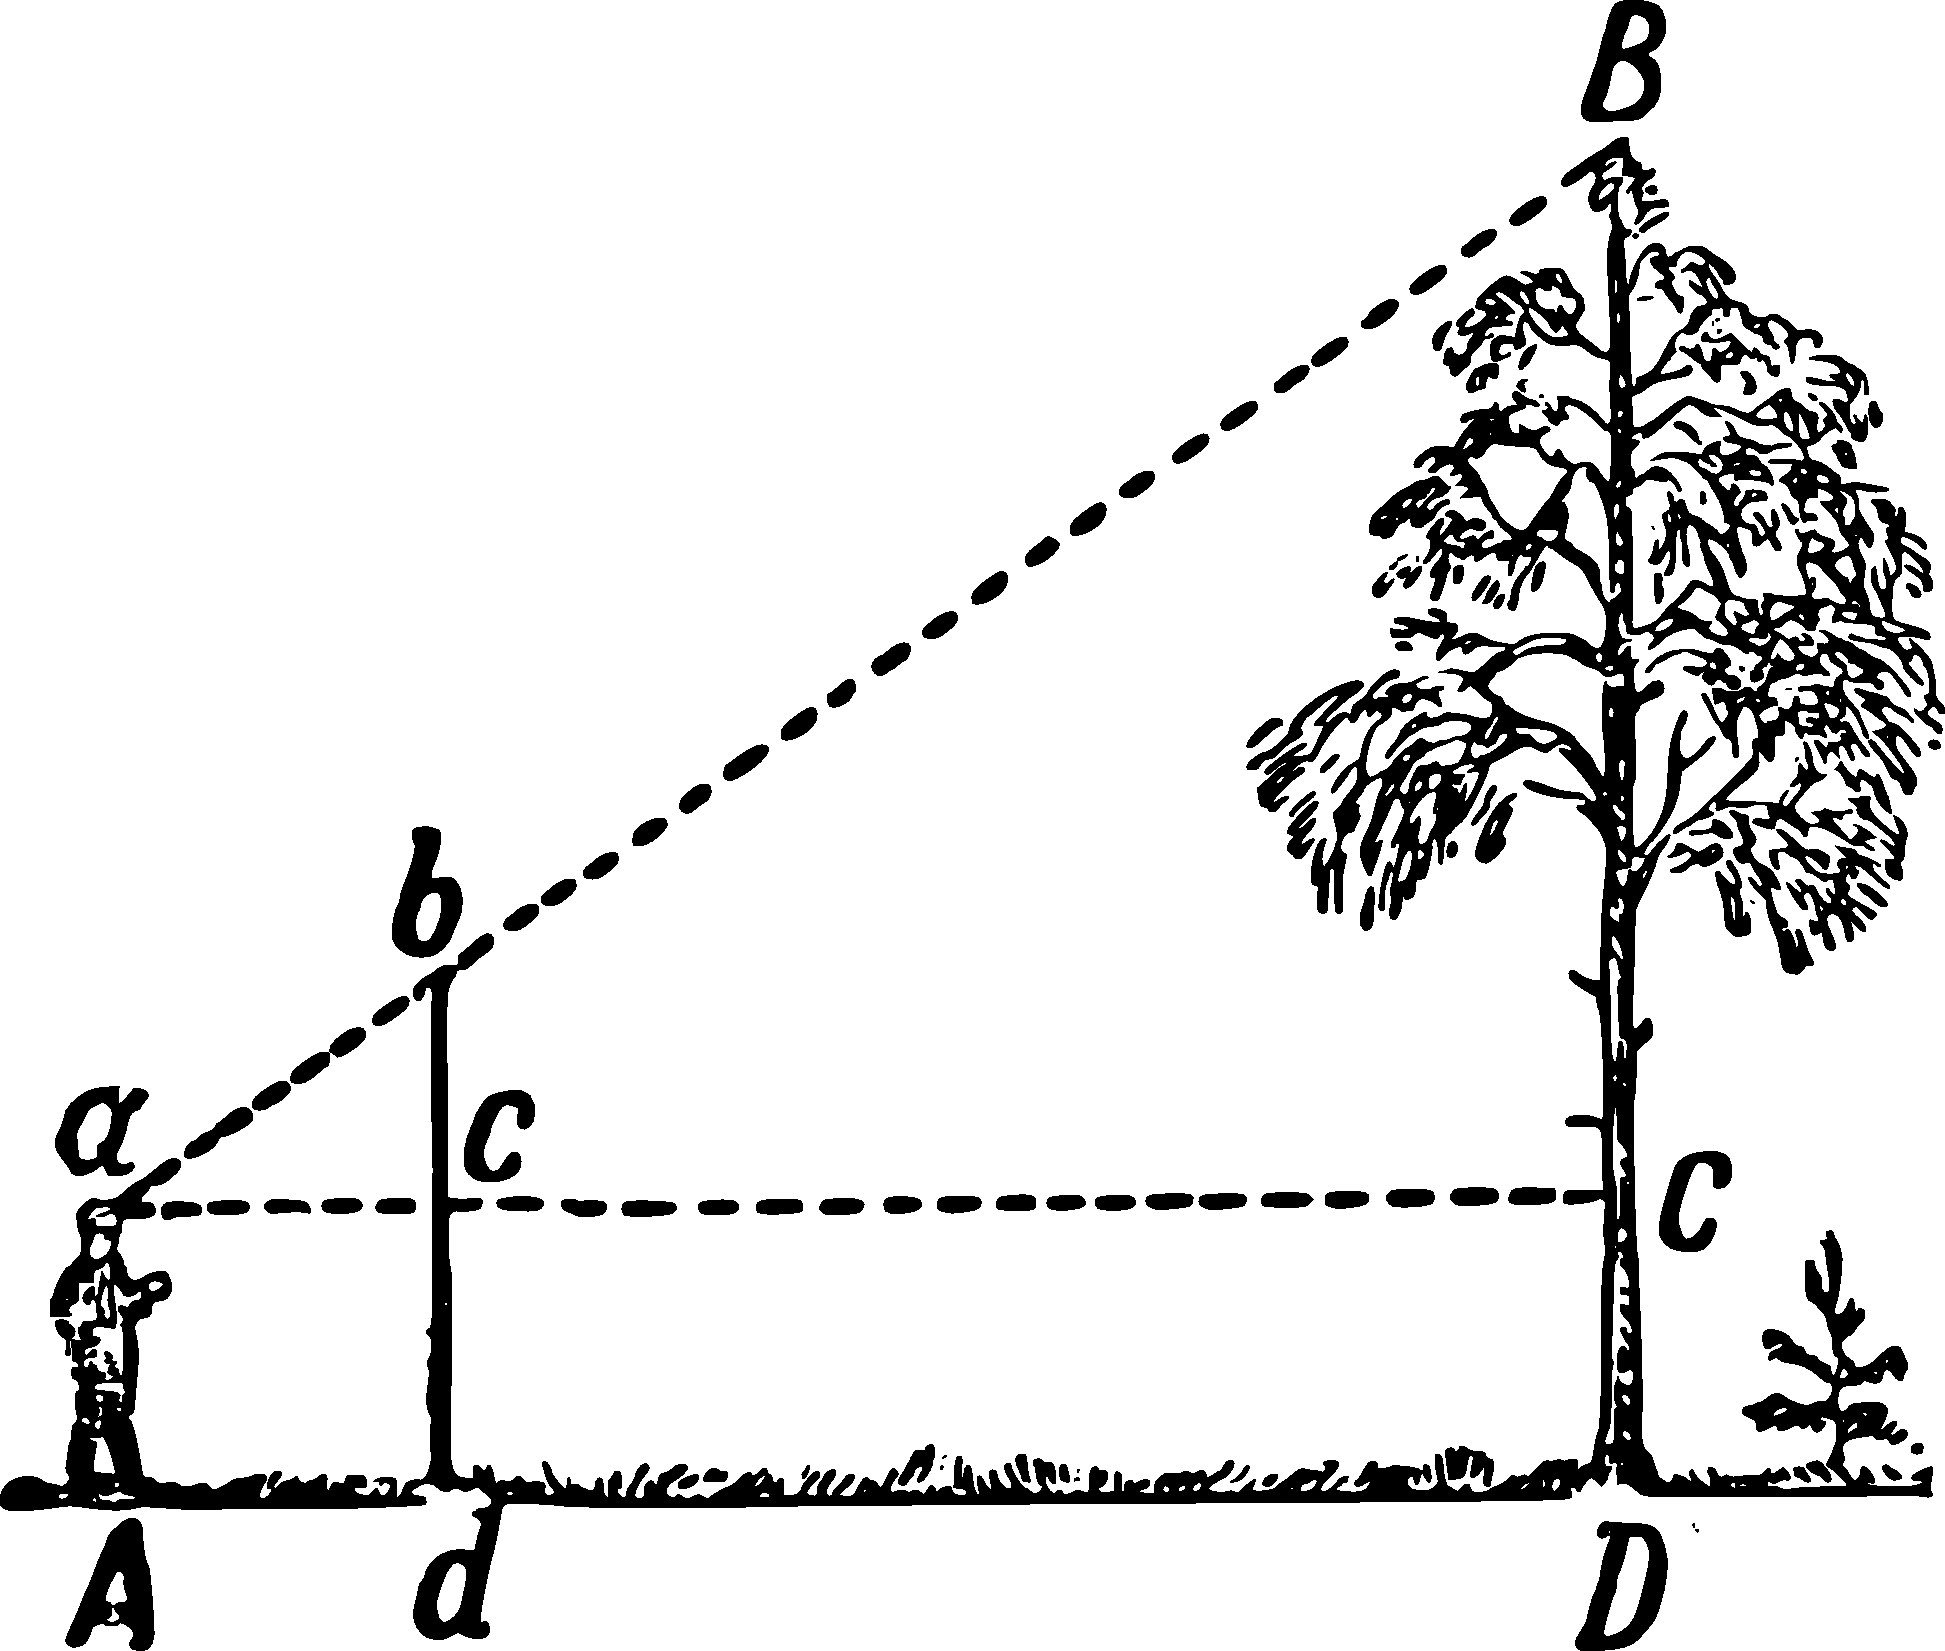
\includegraphics[width=0.6\textwidth]{figures/ch-01/fig-01-08.pdf}
\sidecaption{Measuring the height of the trees with a pole.\label{fig-01-08}}
\end{figure}

This method works as follows: Armed with a pole taller than your own height, drive it into the ground vertically at some distance from the tree being measured (see \figr{fig-01-08}). Step back from the pole along the line $dD$ until you reach point $A$, from where, looking at the top of the tree, you'll see the upper point $B$ of the pole aligned with it. Then, without changing the position of your head, look along the horizontal line $aC$, noting the point $C$ where your line of sight intersects the pole and the tree trunk. Ask your assistant to mark these points, and the observation is complete. Then, based on the similarity of triangles $abc$ and $aBC$, calculate $BC$ from the proportion 
\begin{equation*}%
\frac{BC}{bc} = \frac{aC}{ac},
\end{equation*}
and thus
\begin{equation*}%
BC = bc \cdot \frac{aC}{ac}
\end{equation*}
The distances $bc$, $aC$, and $ac$ can be easily measured directly. To obtain the actual height of the tree, add the distance $BC$ to the distance $CD$, which is also measured directly.

To determine the number of trees, the senior sergeant ordered the soldiers to measure the area of the forest. Then he counted the number of trees in a small area measuring 50 by 50 meters and multiplied accordingly.

Based on all the data collected by the scouts, the unit commander determined where and what kind of bridge needed to be built. The bridge was completed on time, and the combat mission was successfully accomplished!\sidenote{The episodes of the Great Patriotic War described here and further are narrated by A. Demidov in the journal \emph{Military Knowledge} No. 8, 1949, in the article \emph{River Reconnaissance.}\label{ref-21}}

\clearpage

\section{Using a Notebook}
\label{sec-1.5}

As a device for an approximate estimate of the inaccessible height, you can also use your pocket back book, if it is equipped with a pencil stuck in a cover or a loop with a book. It will help you to build in space those two similar triangles, from which the desired height is obtained. The book should be held near the eyes as shown in the simplified \figr{fig-01-09}. It should be in the vertical book so that, looking from the point $a$, you can see the top of the tree $B$ covered with the tip of the pencil $b$. Then, due to the similarity of the triangles $abc$ and $aBC$, the height of the $BC$ will be determined from the proportion
\begin{equation*}%
\frac{BC}{bc} = \frac{aC}{ac}.
\end{equation*}
The distances of $bc$, $ac$ and $aC$ are measured directly. To the resulting value of the $BC$, add the length of $CD$, which is, on level ground, the height of the eyes above the ground


\begin{figure}[h!]
\centering
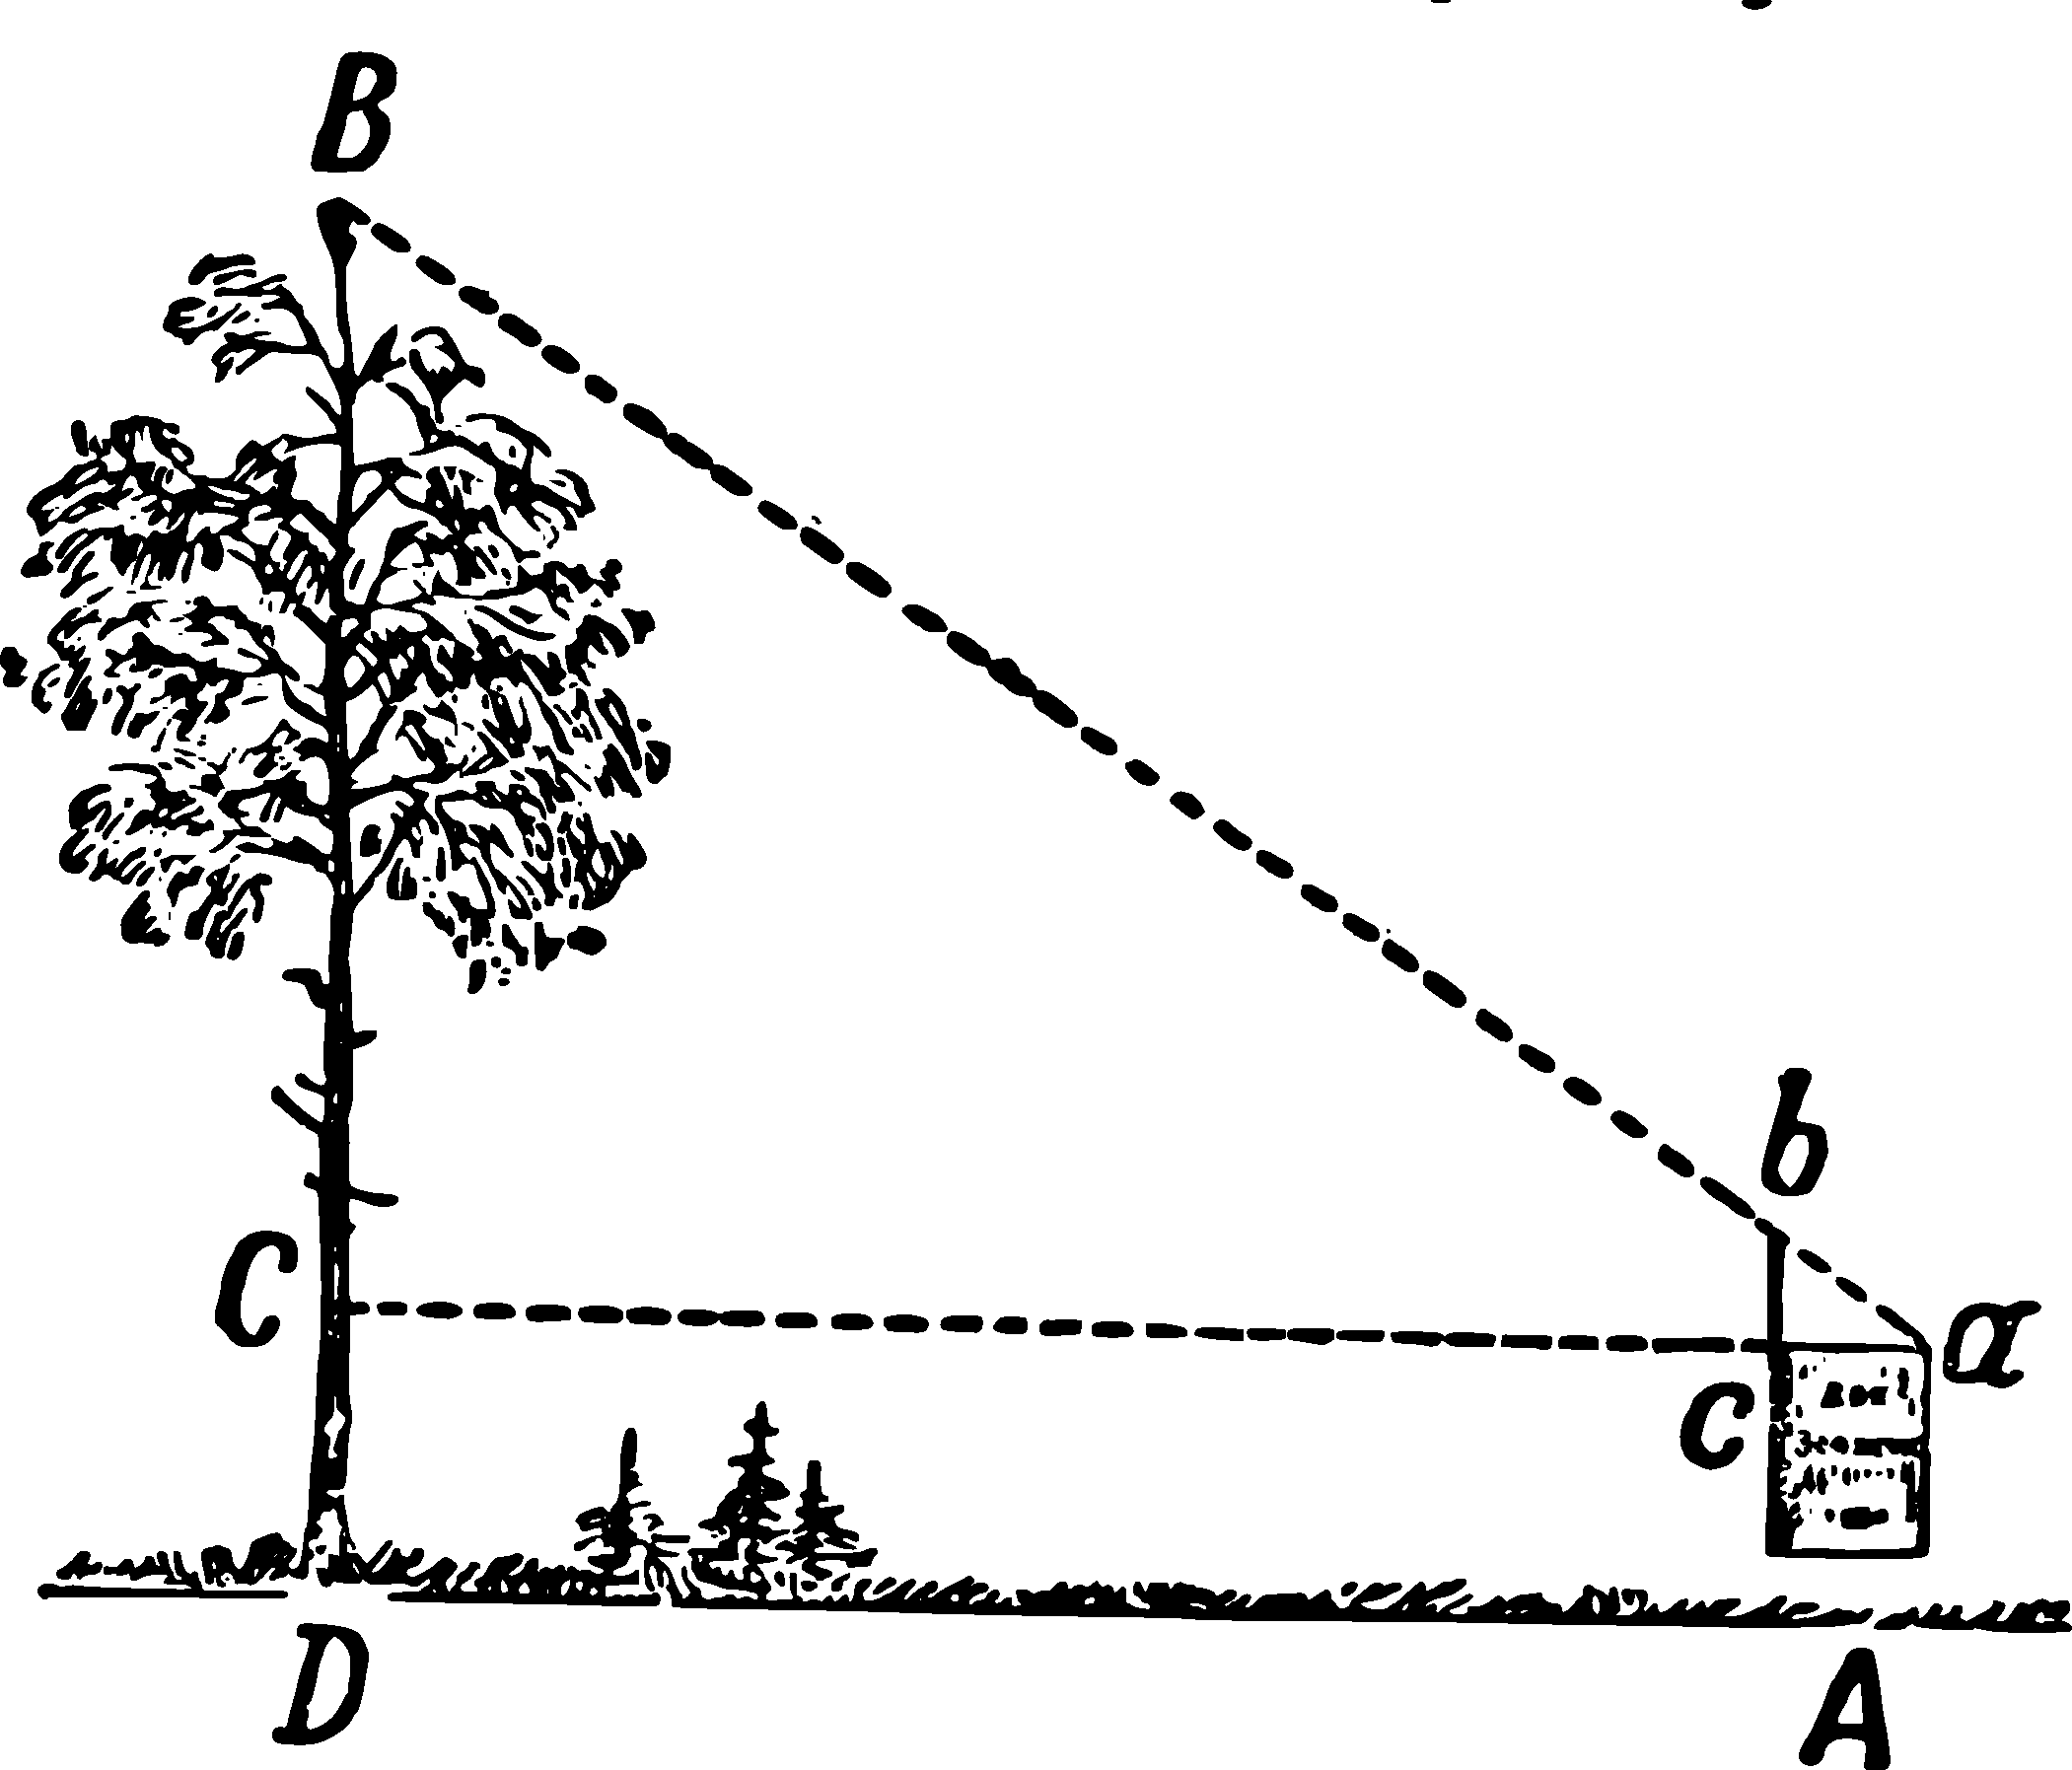
\includegraphics[width=0.6\textwidth]{figures/ch-01/fig-01-09.pdf}
\sidecaption{Height measurement using a notebook.\label{fig-01-09}}
\end{figure}

Since the width of the $ac$ book is unchanged, if you always stand at the same distance from the measured tree (for example, \SI{10}{\meter}), the height of the tree will depend only on the extended part of the pencil. Therefore, you can calculate in advance what height corresponds to a particular extension, and put these numbers on the pencil. Your notebook will then turn into a simplified altimeter, since you can use it to determine heights immediately, without calculations.





\section{Without Approaching The Tree}
\label{sec-1.6}

Sometimes it may be inconvenient to get close to the base of the tree being measured. Can its height still be determined in such a case?

Absolutely. For this purpose, a clever device has been devised, which, like the previous ones, is easy to make by yourself. Two planks, $ab$ and $cd$ (top of \figr{fig-01-10}), are fastened together at right angles so that $ab$ equals $bc$, and $bd$ equals half of $ab$. That's the whole device. 

To measure height with it, hold it in your hands, directing plank CD vertically (for which it has a plumb line with a weight), and stand precisely in two places: first (\figr{fig-01-10}) at point $A$, where the device is positioned with end $c$ up, and then at point $A'$, a bit farther away, where the device is held with end $d$ up. Point $A$ is chosen so that, looking from $a$ to the end of $a$, it is seen on the same line as the top of the tree. Point $A'$ is found so that, looking from $a'$ to point $d'$, it is seen coinciding with $B$. 

The discovery of these two points $A$ and $A'$\sidenote{These points must necessarily lie in a straight line with the base of the tree.} constitutes all the measurement because the desired part of the tree's height, $BC$, is equal to the distance $DA'$. The equality follows easily from the fact that $aC = BC$ and $a'C = 2BC$; thus,
\begin{equation*}%
a'C - aC = BC.
\end{equation*}


\begin{figure}[h!]
\centering
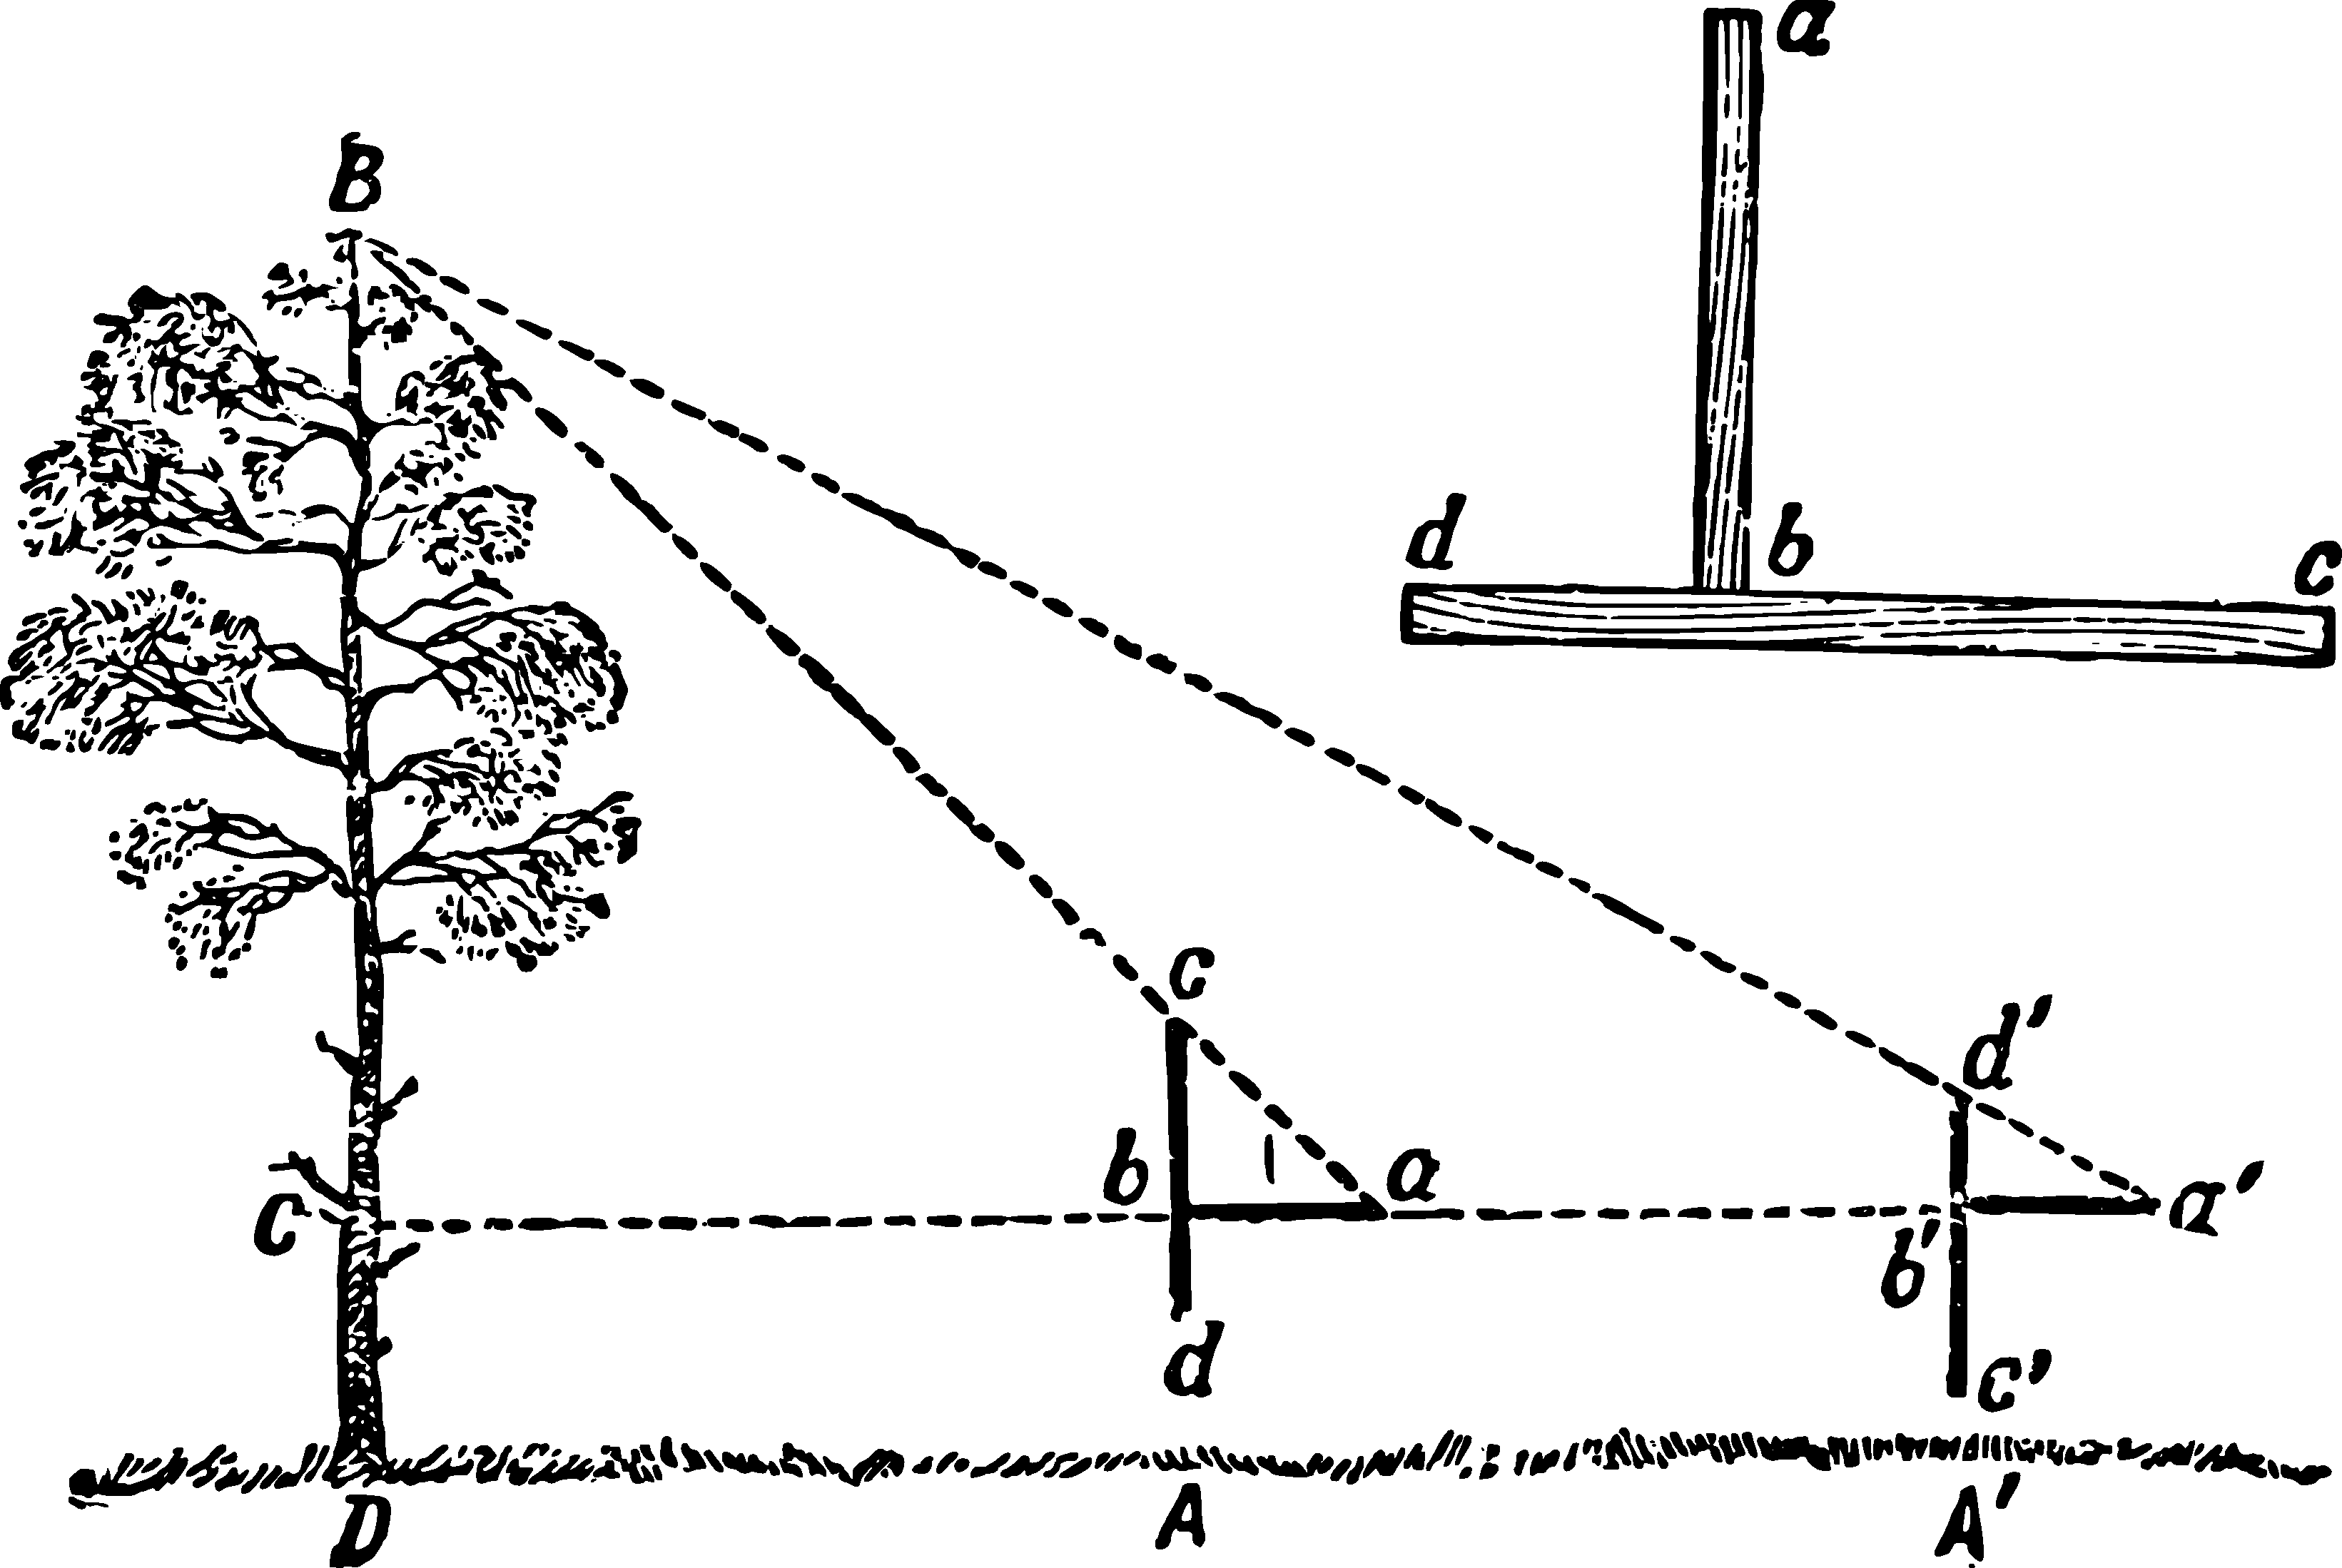
\includegraphics[width=0.8\textwidth]{figures/ch-01/fig-01-10.pdf}
\sidecaption{The use of a simple altimeter consisting of two planks.\label{fig-01-10}}
\end{figure}




You can see that using this simple device, we measure the tree's height without approaching closer than its height. It goes without saying that if it's possible to approach the trunk, it's sufficient to find just one of the points -- $A$ or $A'$ -- to determine its height.

Instead of two planks, you can use four pins, arranging them on a board properly; in this form, the ``device'' is even simpler.

%\clearpage

\section{Forest Rangers' Altimeter}
\label{sec-1.7}

It's time to explain how the ``real'' altimeters, used in practise by forest workers, are constructed. I'll describe one of these altimeters, slightly modifying it so that the device can be easily crafted at home. 

\begin{figure}[h!]
\centering
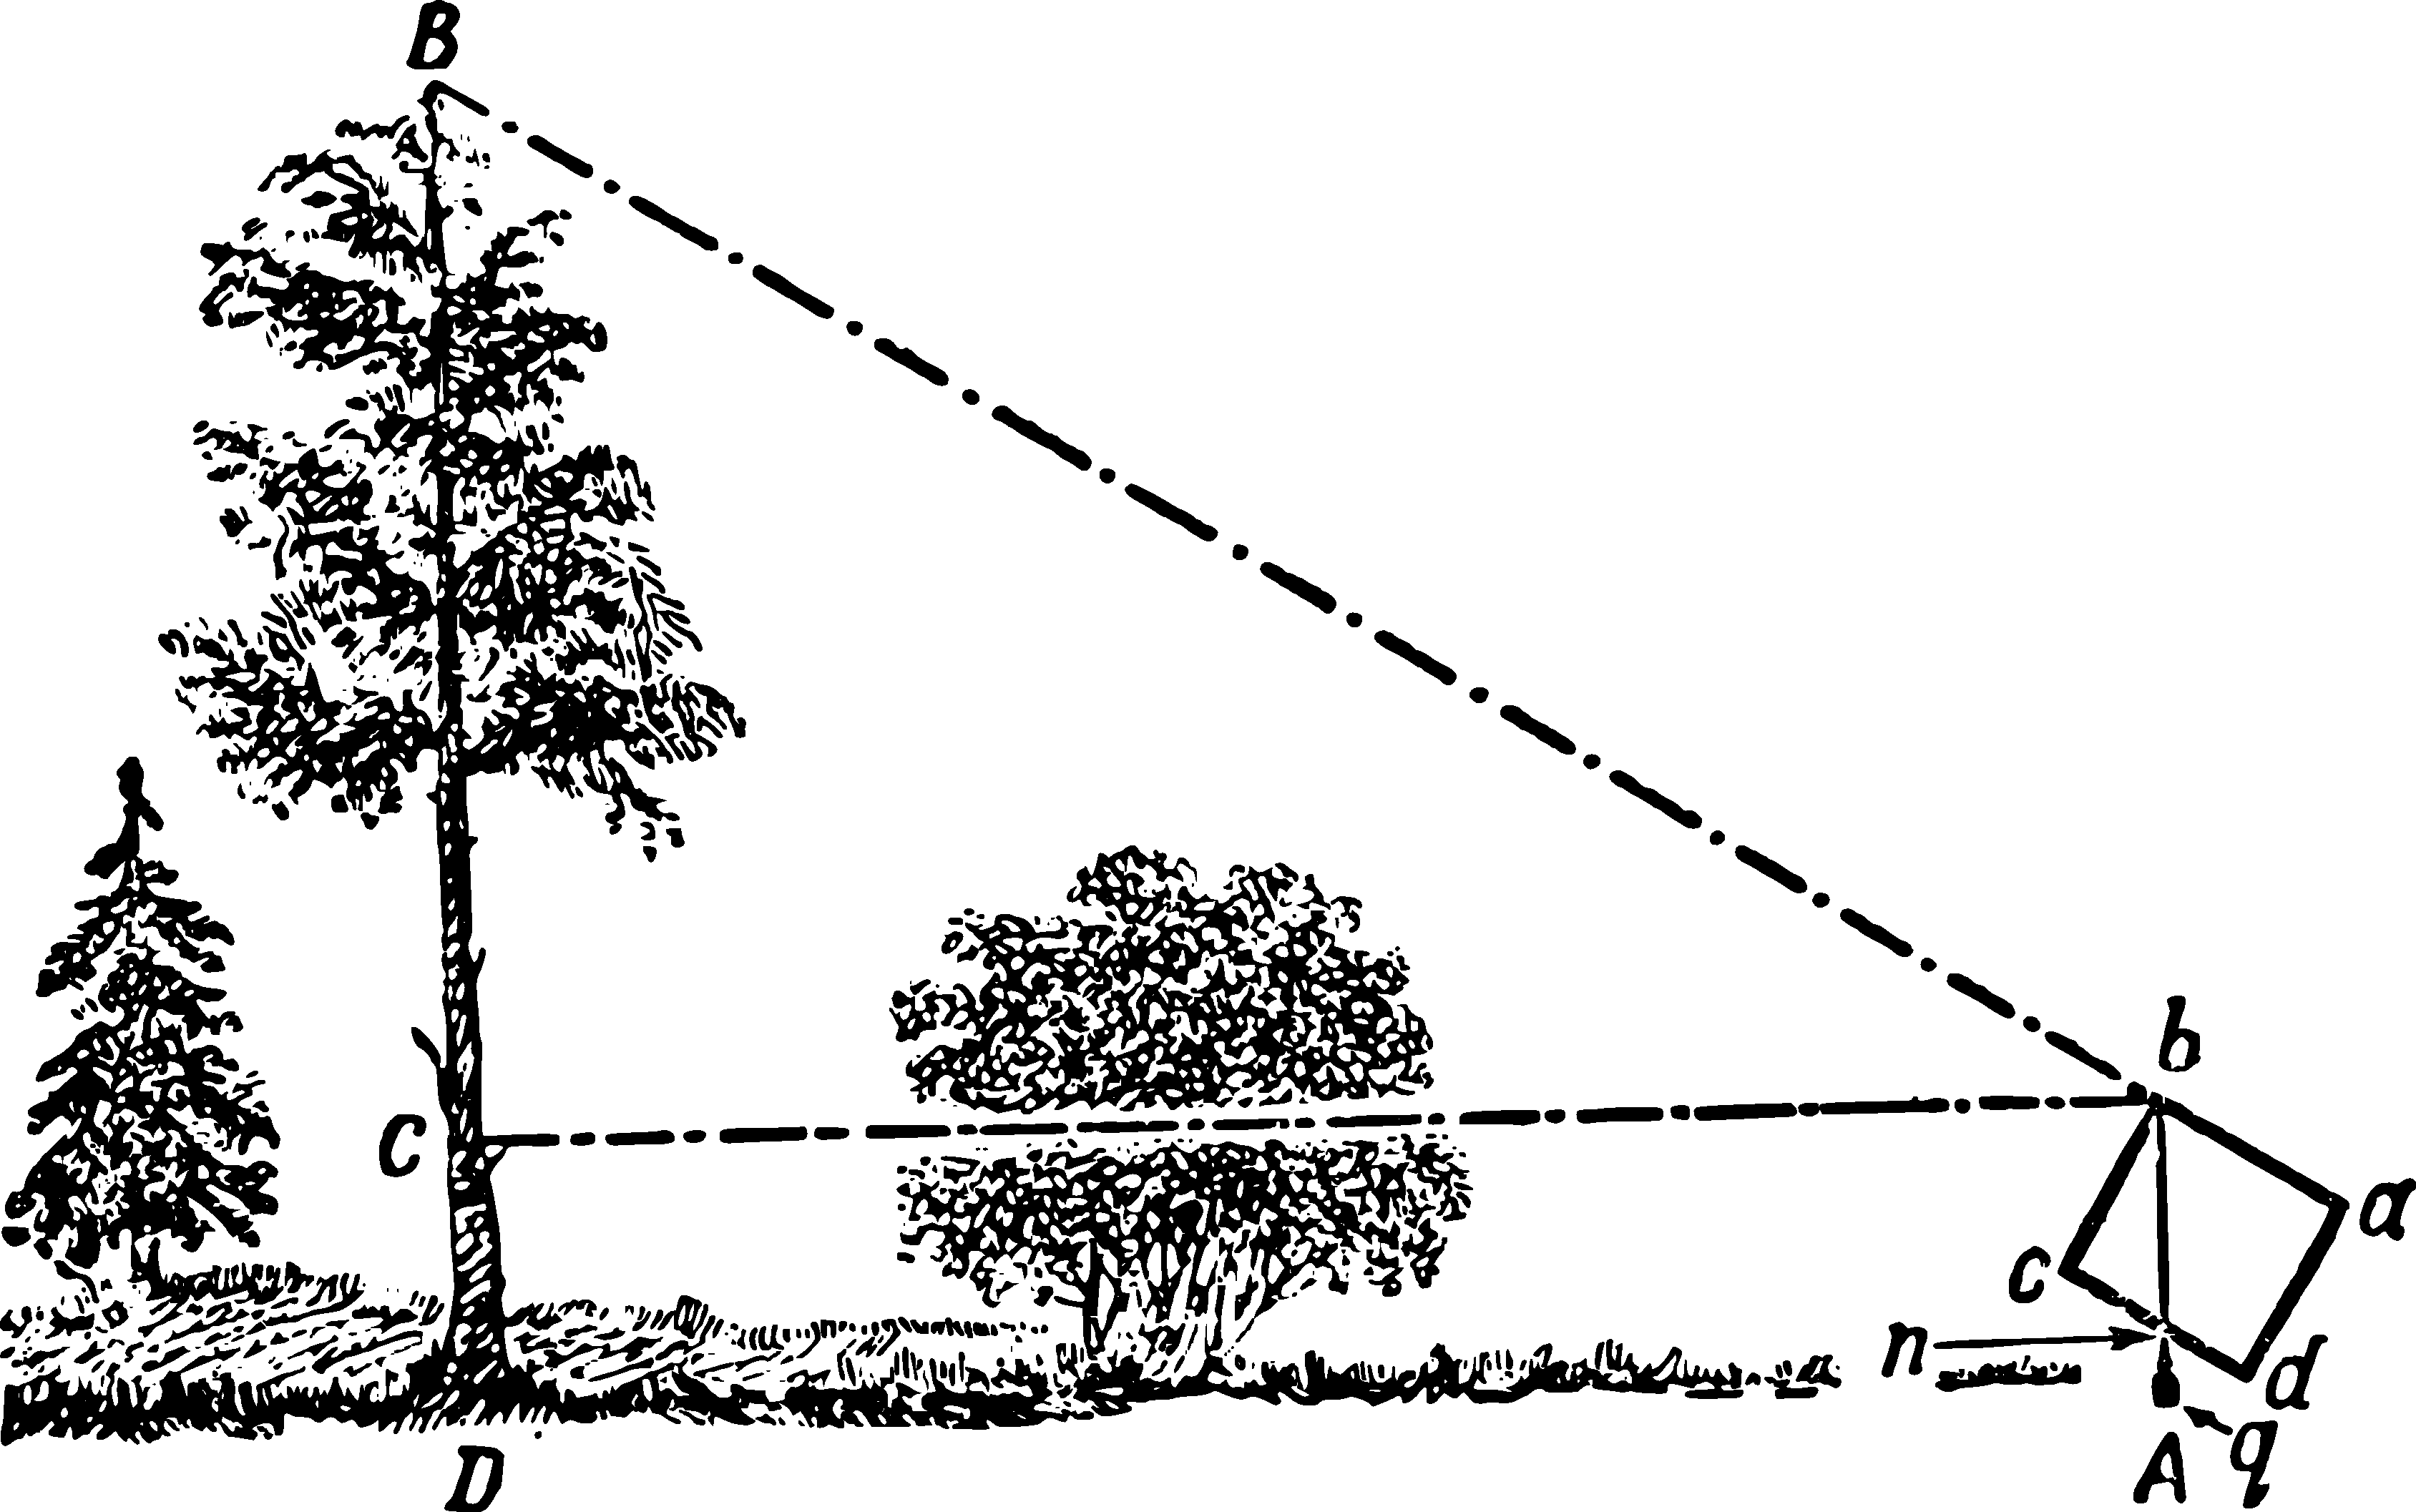
\includegraphics[width=\textwidth]{figures/ch-01/fig-01-11.pdf}
\sidecaption{The scheme of using the altimeter of foresters.\label{fig-01-11}}
\end{figure}


The essence of the device is visible in \figr{fig-01-11}. A cardboard or wooden rectangle, $abcd$, is held in the hand so that, looking along edge $ab$, the tip $B$ of the tree is in line with it. A weight, $q$, is suspended from point $b$ on a thread. We note the point $n$ where the thread intersects line $dc$. Triangles $bBC$ and $bnc$ are similar because they are both rectangular and have equal acute angles $bBC$ and $bnc$ (with corresponding parallel sides). Therefore, we can write the proportion:
\begin{align*}%
\frac{BC}{nc} & = \frac{bC}{bc}; \,\, \text{hence} \\
BC & = bC \cdot \frac{nc}{bc}.
\end{align*}
Since $bC$, $nc$, and $bc$ can be measured directly, it is easy to obtain the desired height of the tree by adding the length of the lower part $CD$ to the trunk (the height of the device above the ground). 

A few details remain to be added. If the edge of the board $bc$ is made, for example, exactly \SI{10}{\centi\meter}, and centimeter divisions are marked on edge $dc$, then the ratio $nc/bc$ will always be expressed as a decimal fraction, directly indicating what fraction of the distance $bC$ represents the height of the tree $BC$. For example, let's say the thread stops against the 7th division mark (i.e., $nc = \SI{7}{\centi\meter}$); this means that the height of the tree above eye level is 0.7 times the observer's distance from the trunk.

\begin{figure}[h!]
\centering
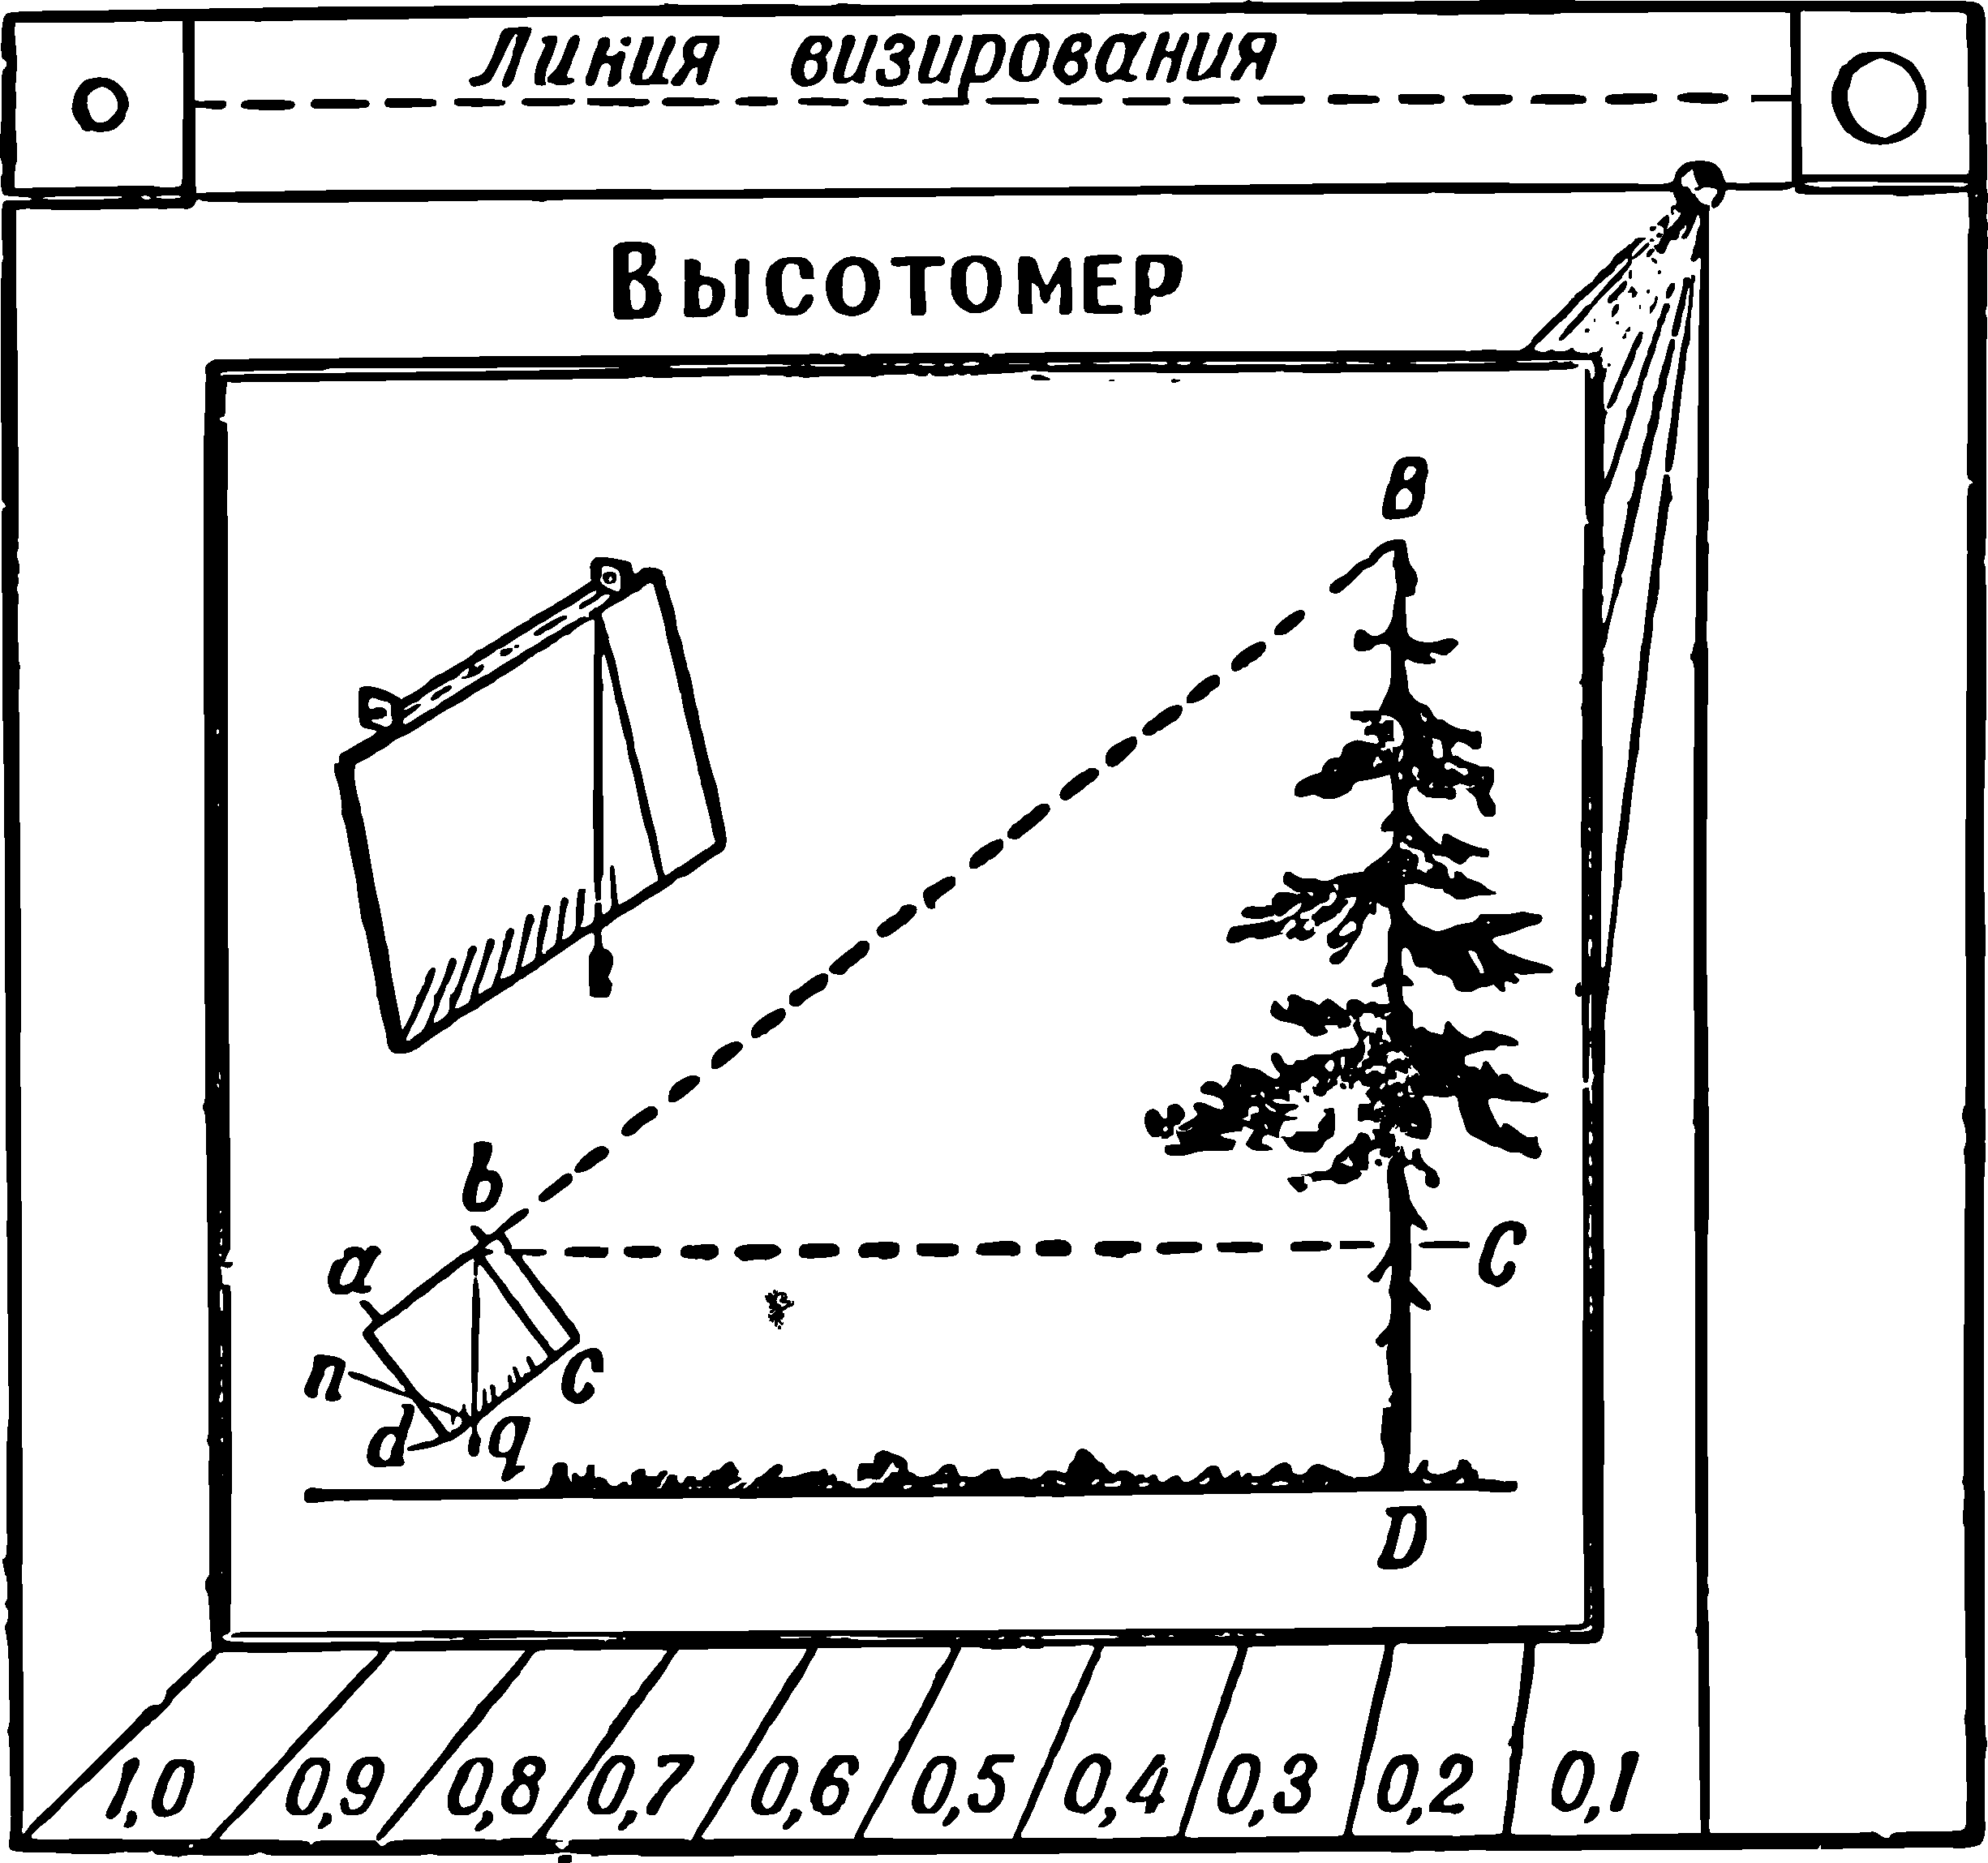
\includegraphics[width=0.7\textwidth]{figures/ch-01/fig-01-12.pdf}
\sidecaption{The forest rangers' altimeter.\label{fig-01-12}}
\end{figure}

The second improvement relates to the method of observation: to make it convenient to look along line $ab$, you can fold down two squares with holes drilled in them at the upper corners of the cardboard rectangle: one smaller one for the eye and one larger one for sighting the tree top (see \figr{fig-01-11}). Further enhancement is represented by the device shown almost to scale in \figr{fig-01-12}. It is easy and quick to make it in this form; no special skill is required. Occupying little space in the pocket, it will provide you with the ability to quickly determine the heights of encountered objects during excursions—trees, poles, buildings, and so on. (This tool is part of the \emph{Geometry in the Open Air} kit developed by the author of this book.)

%\clearpage


\ques Is it possible to use the altimeter described now to measure trees that cannot be approached closely? If possible, what should be done In such cases?


\ans The device should be aimed at the top of the tree $B$, as shown in \figr{fig-01-13}, from two points, $A$ and $A'$. 

\begin{figure}[h!]
\centering
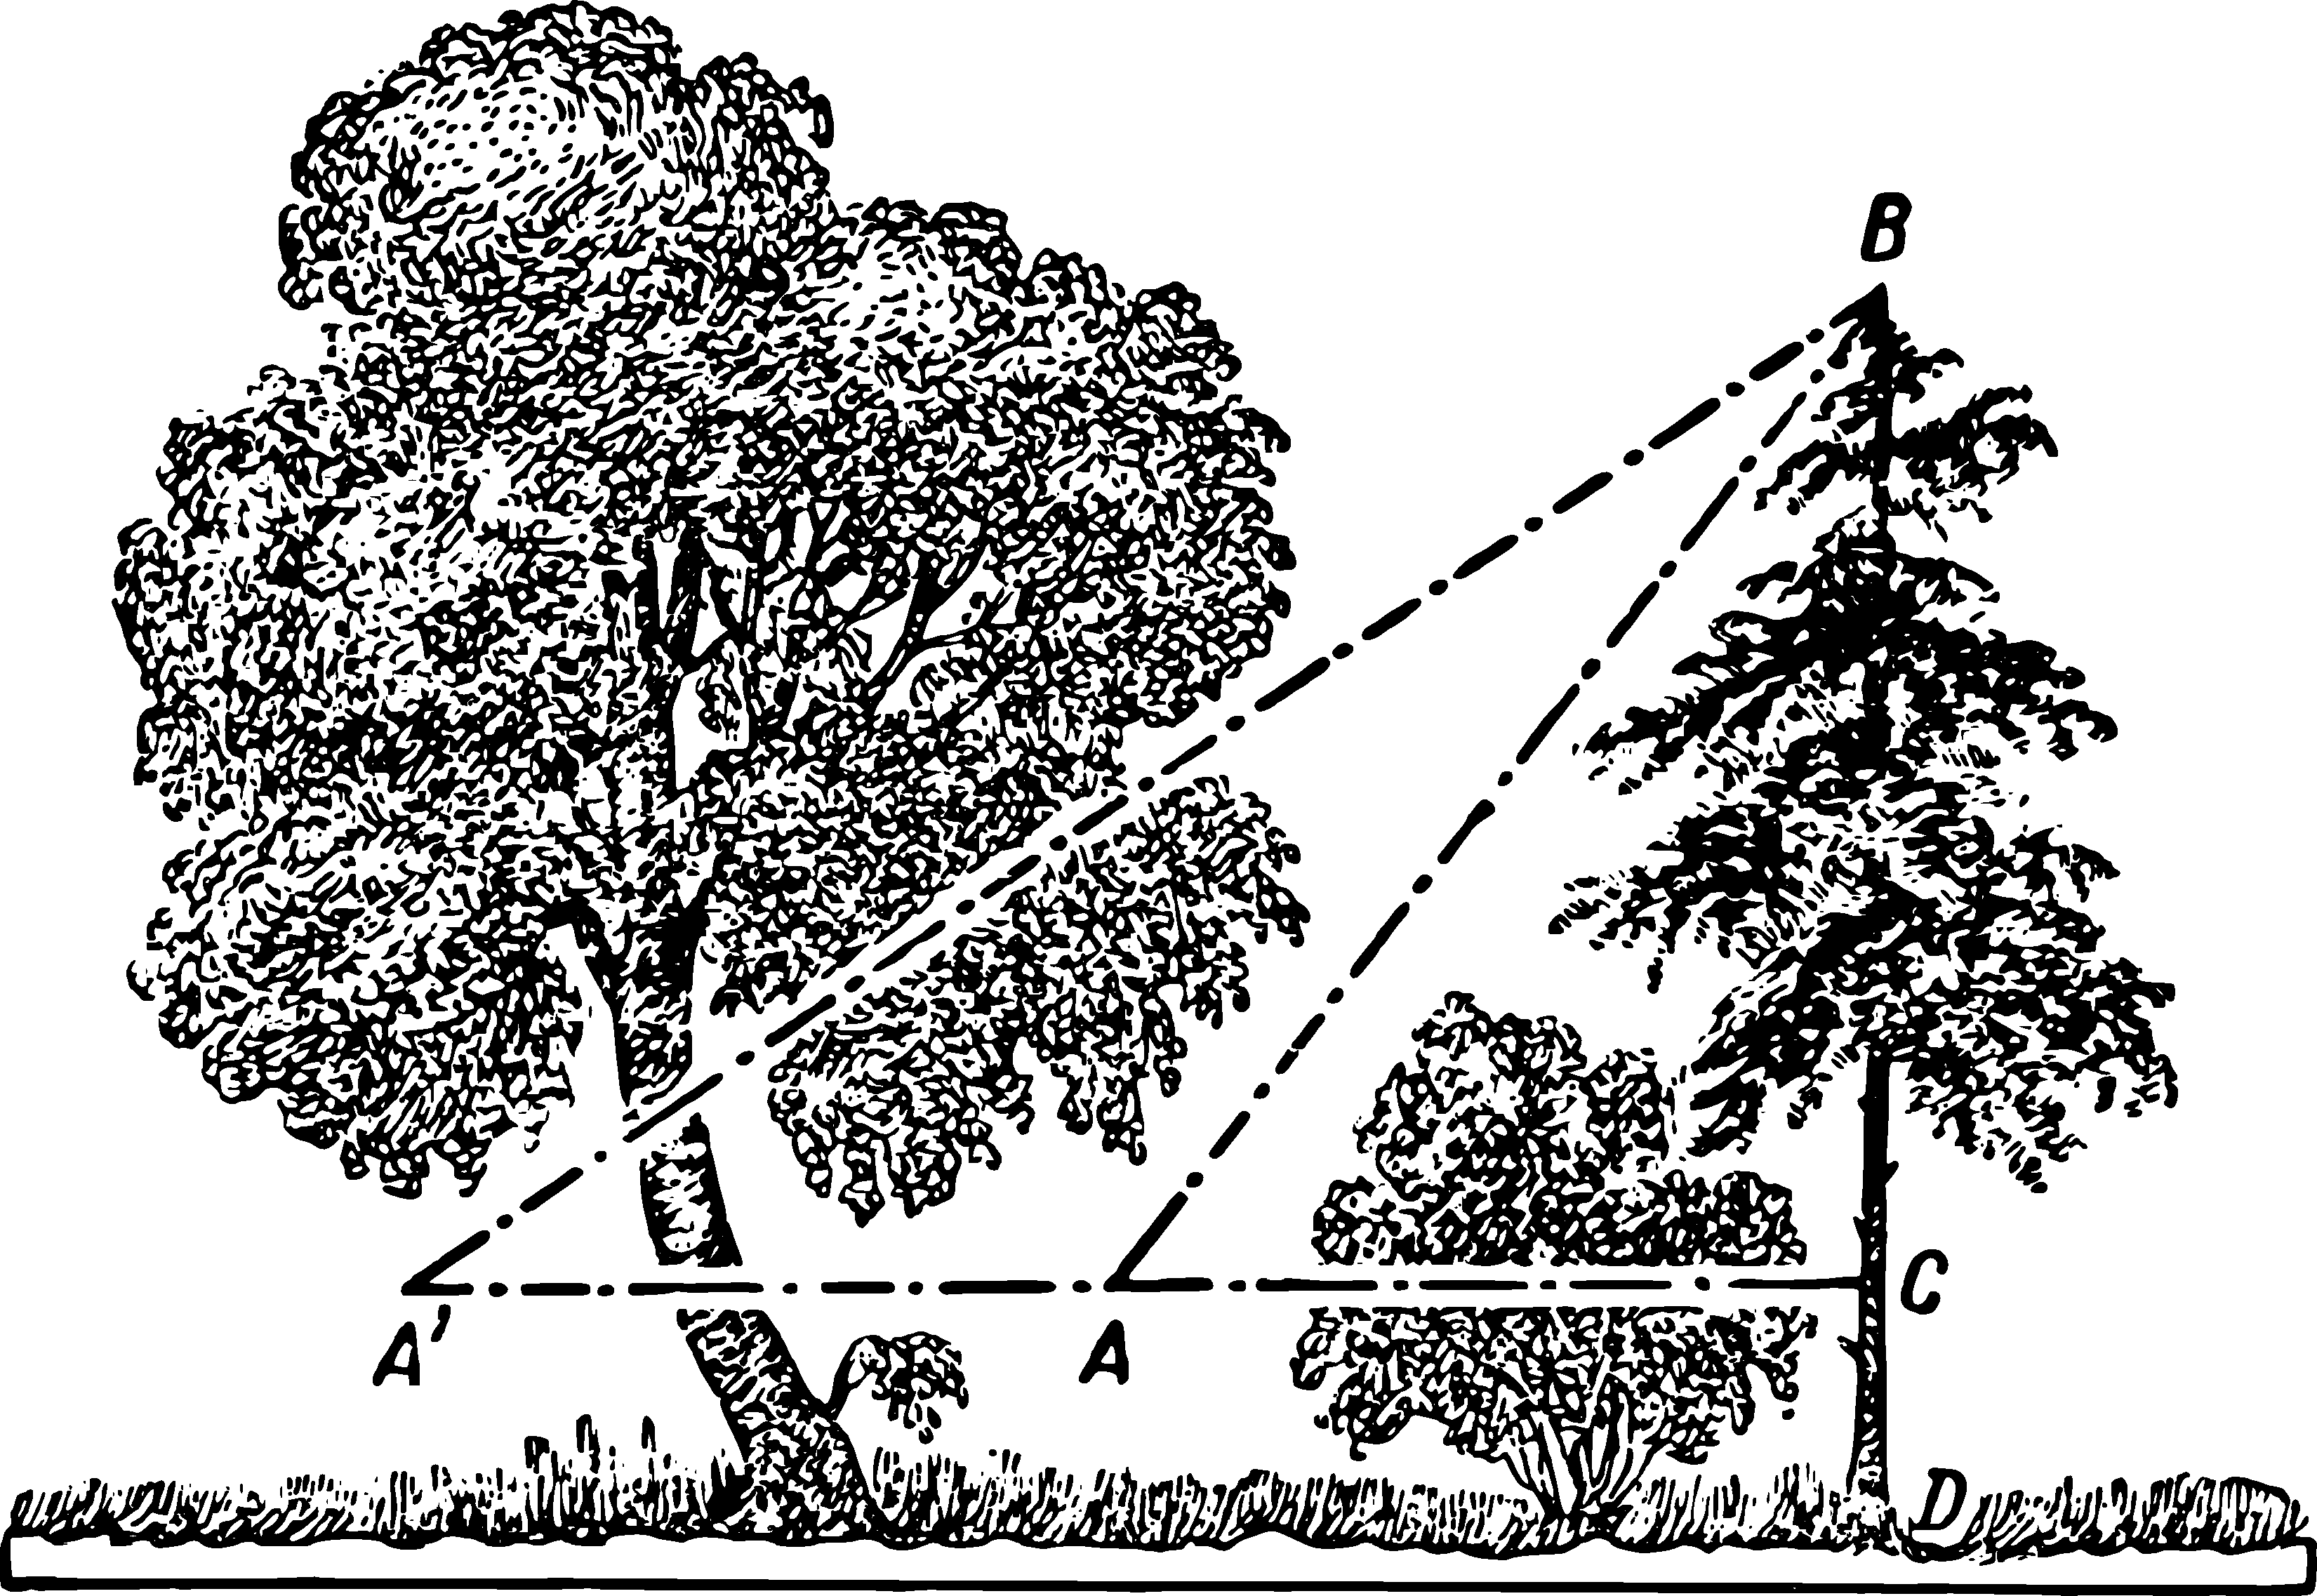
\includegraphics[width=0.9\textwidth]{figures/ch-01/fig-01-13.pdf}
\sidecaption[][-1cm]{How to measure the height of a tree without approaching it.\label{fig-01-13}}
\end{figure}

Let's say at point $A$ we determined that $BC = 0.9\,AC$, and at point $A'$ we determined that $BC = 0.4\,A'C$. Then we know that:
\begin{equation*}%
AC = \frac{BC}{0.9},\quad   A'C  = \frac{BC}{0.4} 
\end{equation*}
So that we can write
\begin{equation*}%
AA' = A'C - AC = \frac{BC}{0.4} - \frac{BC}{0.9} = \frac{25}{18} \,BC.
\end{equation*}
Hence,
\begin{align*}%
AA' & = \frac{25}{18} \,BC, \\ 
\therefore BC & = \frac{18}{25} \,AA' \\
& = 0.72 \, AA'.
\end{align*}
You can see that by measuring the distance $AA'$ between both observation points and taking a certain fraction of this value, we can determine the desired and inaccessible height.

\section{Using a Mirror}
\label{sec-1.8}


\ques Here's another unconventional method for determining the height of a tree using a mirror. At some distance (see \figr{fig-01-14}) from the tree being measured, on level ground at point $C$, place a small mirror horizontally and step back to point $D$, from where the observer can see the top of tree's point $A$ in the mirror. Then, the tree ($AB$) is as many times taller than the observer's height ($ED$) as the distance $BC$ from the mirror to the tree is greater than the distance $CD$ from the mirror to the observer. Why?

\begin{figure}[h!]
\centering
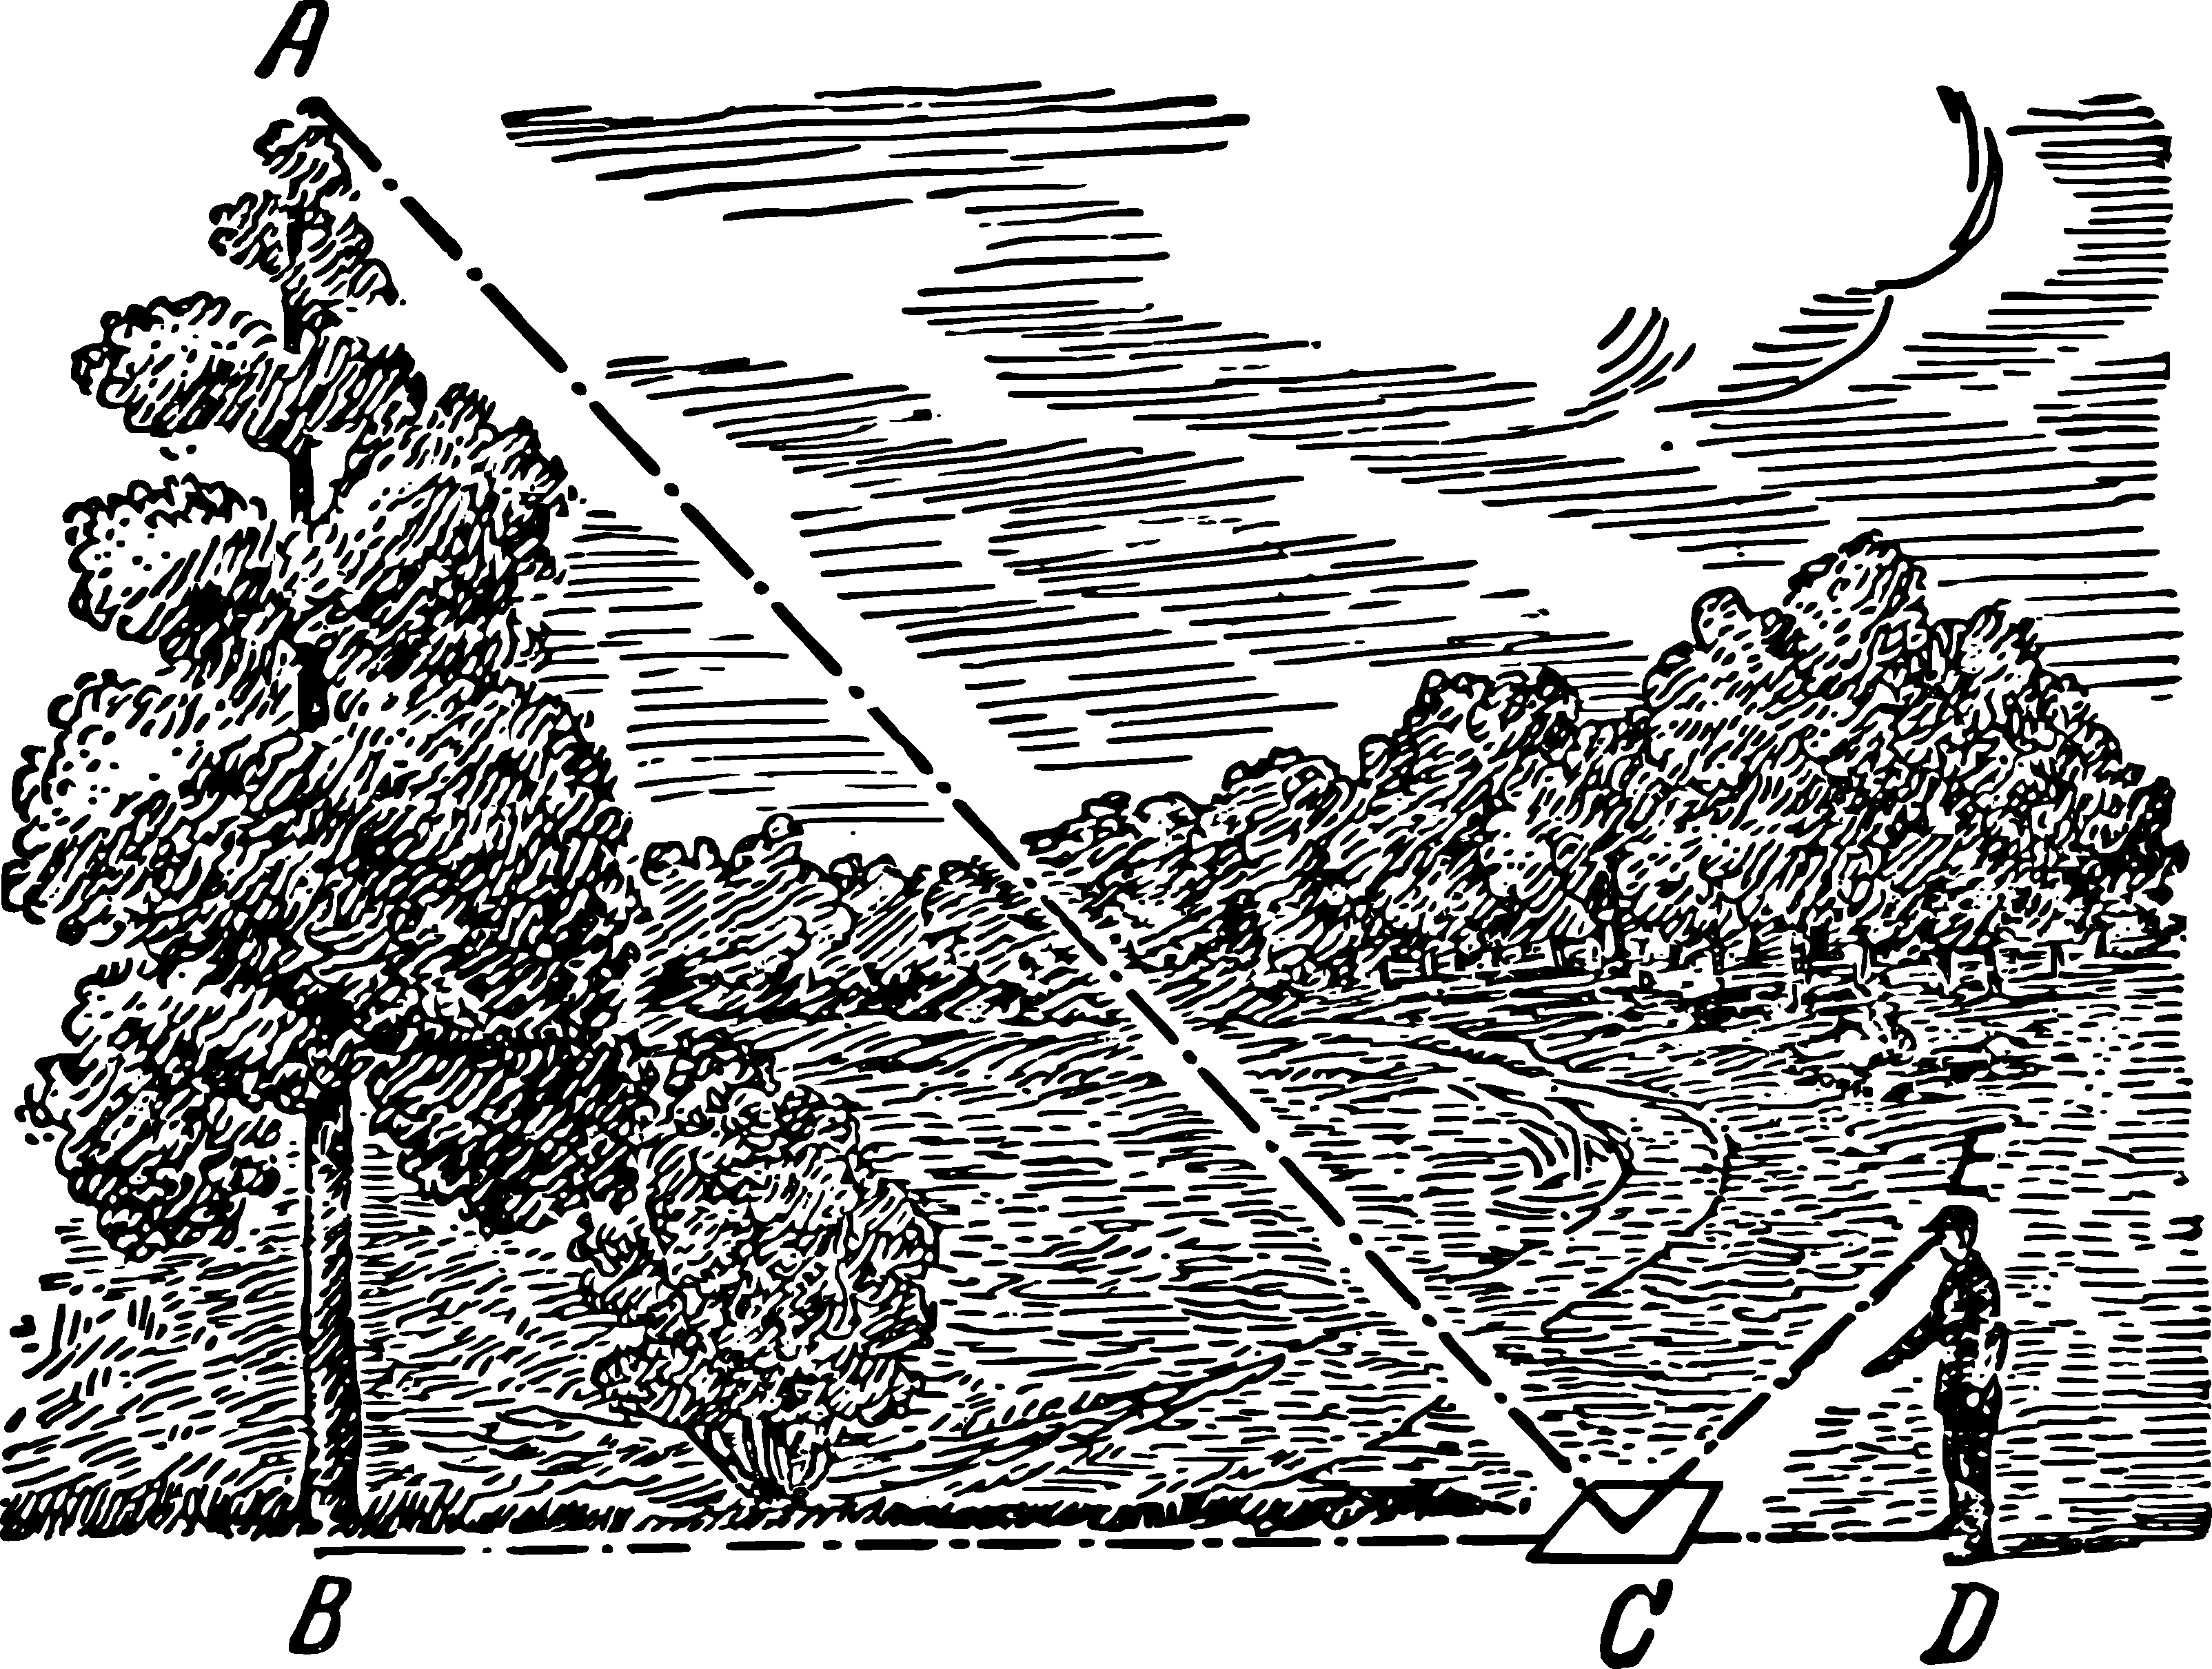
\includegraphics[width=0.9\textwidth]{figures/ch-01/fig-01-14.pdf}
\sidecaption[][0cm]{Height measurement using a mirror.\label{fig-01-14}}
\end{figure}


\ans The method is based on the law of reflection of light. The top $A$ (\figr{fig-01-15}) is reflected at point $A'$ in such a way that $AB = A'B$. From the similarity of triangles $BCA'$ and $CED$, it follows that 
\begin{equation*}%
\frac{A'B}{ED} = \frac{BC}{CD}. 
\end{equation*}
In this, simply replace $A'B$ with $AB$ to justify the relationship stated in the problem. This convenient and effortless method can be applied in any weather, but not in dense vegetation, only to a solitary tree.
\begin{marginfigure}[-4cm]%[h!]
\centering
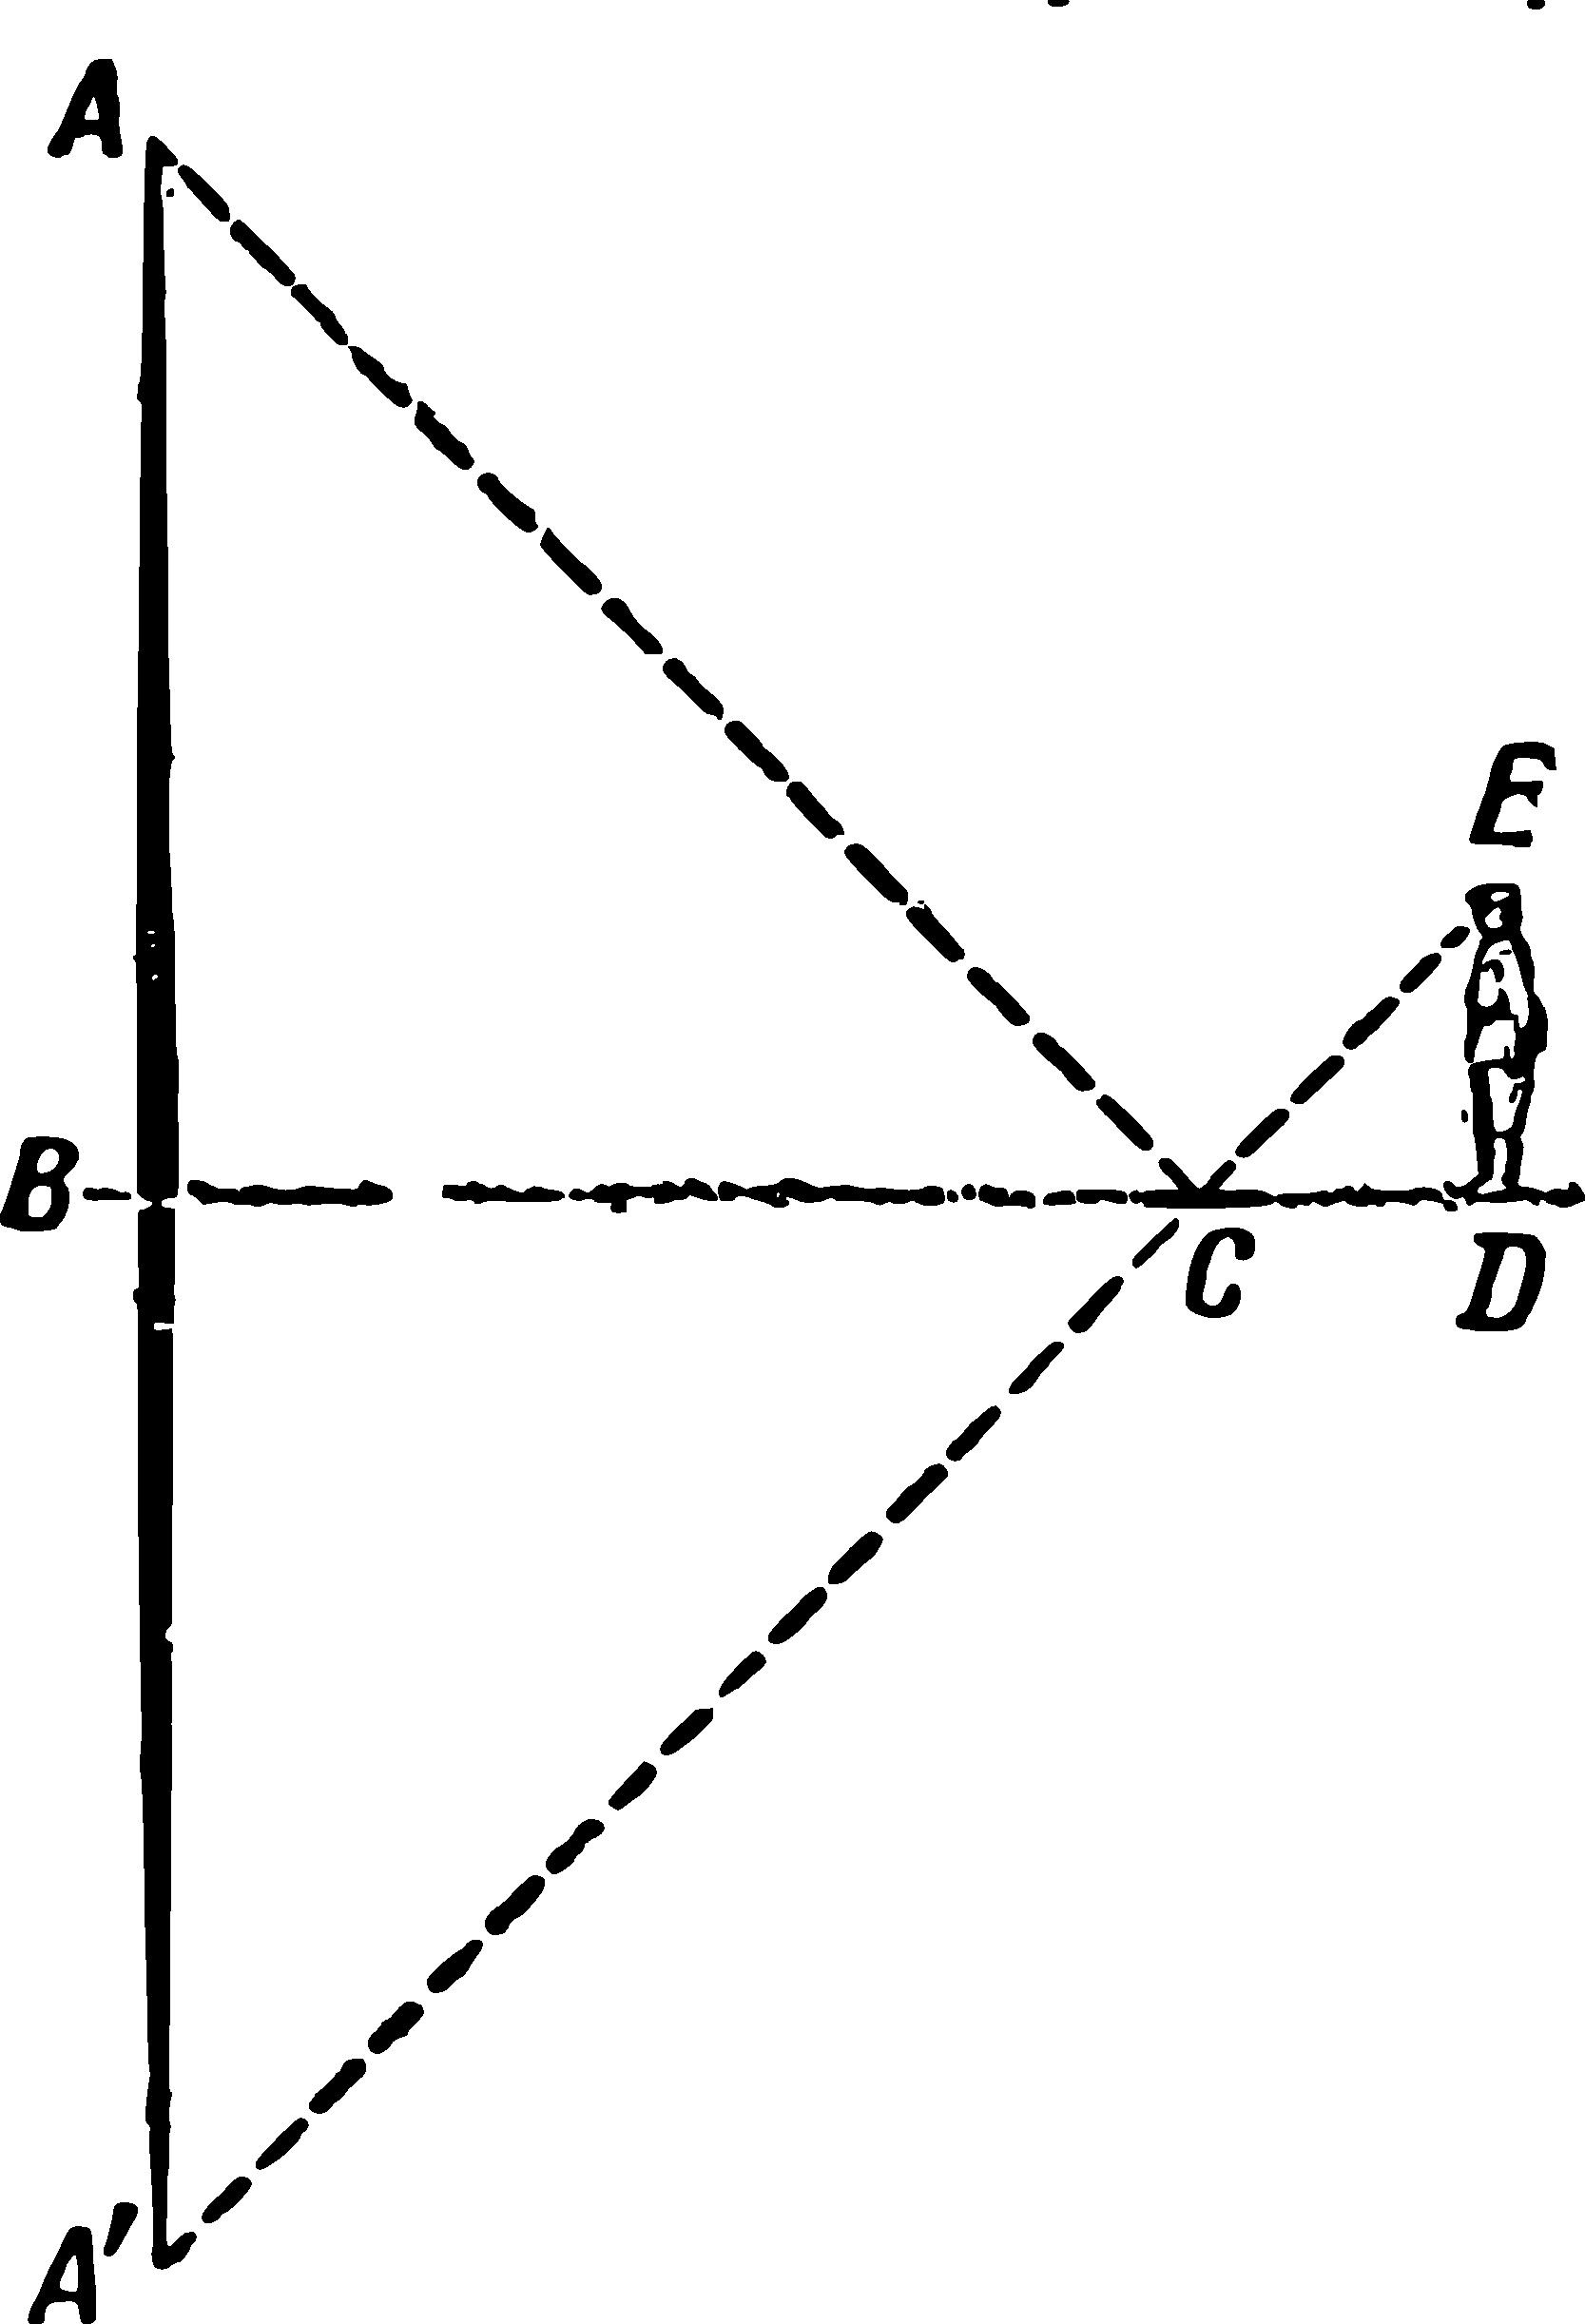
\includegraphics[width=0.9\textwidth]{figures/ch-01/fig-01-15.pdf}
\sidecaption{Geometric construction for the method of measuring the height using a mirror.\label{fig-01-15}}
\end{marginfigure}

%\clearpage 

\ques However, what should be done when it is impossible to approach the tree being measured closely for some reason?\\

\ans This is an ancient problem dating back over 500 years. It is discussed by the medieval mathematician Antonius de Cremona in his work \emph{On Practical Land Measurement} (1400).


The problem is solved by the dual application of the method described earlier -- placing the mirror in two locations. By making the appropriate construction, it is easy to deduce from the similarity of triangles that the sought-after height of the tree is equal to the observer's eye level multiplied by the ratio of the distance between the mirror positions to the difference in distances from the mirror to the observer.

Before concluding the discussion on measuring the height of trees, I propose to the reader another ``forest'' problem.

\section{Two Pines}
\label{sec-1.9}


\ques Two pine trees grow 40 meters apart. You measured their heights: one turned out to be 31 meters tall, while the other, younger one, is only 6 meters tall. Can you calculate the distance between their tops?

\begin{figure}[h!]
\centering
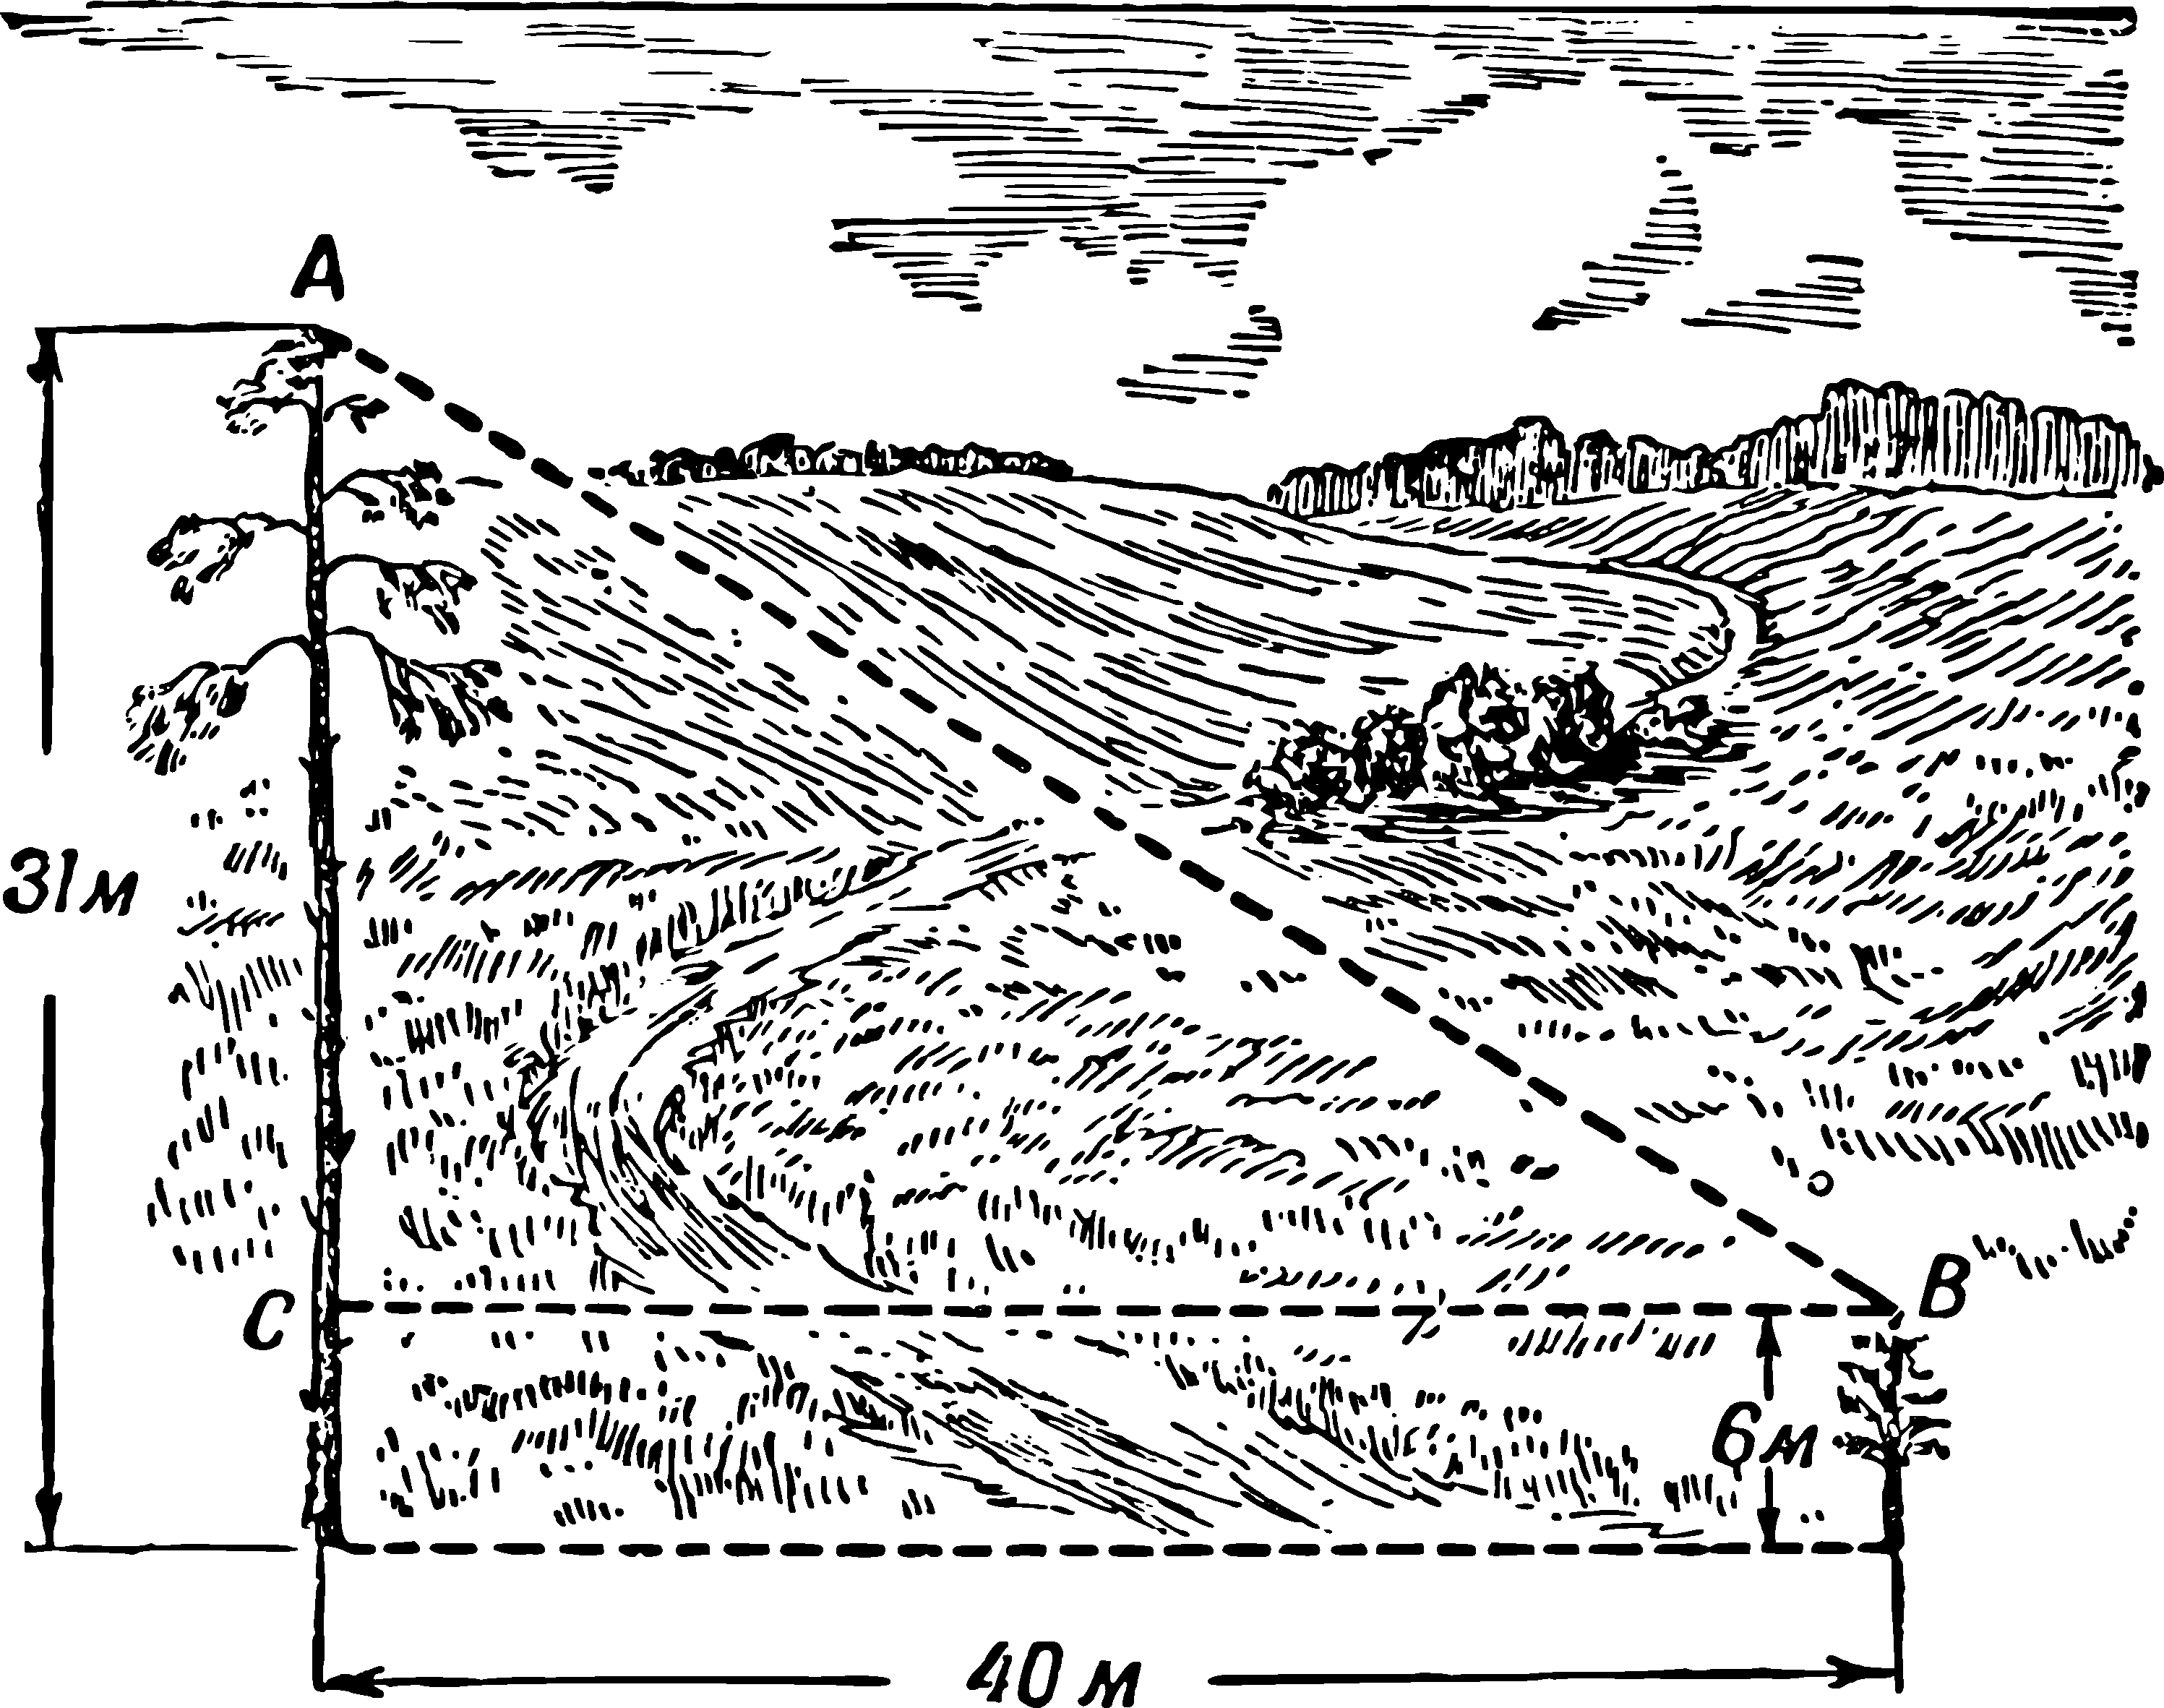
\includegraphics[width=0.9\textwidth]{figures/ch-01/fig-01-16.pdf}
\sidecaption{What is the distance between the tops of the pines?\label{fig-01-16}}
\end{figure}

\ans The desired distance between the tops of the pine trees (see \figr{fig-01-16}) according to the Pythagorean theorem is
\begin{equation*}%
\sqrt{40^{2} + 25^{2}} = \SI{47}{\meter}.
\end{equation*}



\section{The shape of the tree trunk}
\label{sec-1.10}

Now you can already, walking through the forest, determine -- in almost half a dozen different ways -- the height of any tree. It will probably be interesting for you to determine its volume as well, calculate how many cubic meters of wood it contains, and at the same time weigh it. To find out if, for example, it would be possible to take away such a trunk on one cart. Both of these tasks are no longer as simple as determining height; experts have not found ways to accurately resolve it and are content with only a more or less approximate estimate. Even for a felled trunk, which lies in front of you cleared of branches, the task is far from easy.

The thing is, a tree trunk, even the smoothest one without bulges, does not represent either a cylinder, a complete cone, a truncated cone, or any other geometric solid whose volume we can calculate using formulas. The trunk is certainly not a cylinder — it tapers towards the top (it has ``runoff'', as foresters say) — but it is also not a cone because its ``generating line'' is not a straight line, but a curve, and moreover, not a circular arc, but some other curve, convex towards the axis of the tree.\sidenote[][-5cm]{The curve that fits closest to this is called the ``semicubical parabola'' $(y^3 = ax^2)$; the solid obtained by rotating this parabola is called a ``neiloid'' (named after the ancient mathematician Neil, who found a way to determine the length of the arc of such a curve). The shape of a tree trunk grown in the forest approximates that of a neiloid. Calculating the volume of a neiloid is done using advanced mathematical techniques.}

Therefore, a more or less accurate calculation of the volume of a tree trunk can only be done using the tools of integral calculus. To some readers, it may seem strange that the measurement of a simple log requires resorting to the services of higher mathematics. Many think that higher mathematics is only relevant to some special subjects, whereas in everyday life, only elementary mathematics is applicable. This is completely incorrect: one can fairly accurately calculate the volume of a star or a planet using elements of geometry, whereas an exact calculation of the volume of a long log or a beer barrel is impossible without analytical geometry and integral calculus.

However, our book does not assume that the reader is familiar with higher mathematics; therefore, here we will have to be content with only an approximate calculation of the volume of the trunk. We will assume that the volume of the trunk is more or less close either to the volume of a truncated cone, or -- for a trunk with a pointed end — to the volume of a complete cone, or, finally, -- for short logs — to the volume of a cylinder. The volume of each of these three solids can be easily calculated. Could we find a formula for the volume that would be suitable for all three of these named solids for the sake of consistency in calculation? Then we would approximately calculate the volume of the trunk without caring about what it resembles more — a cylinder or a cone, complete or truncated.


\section{Universal Formula}
\label{sec-1.11}

Such a formula exists; moreover, it is not only suitable for cylinders, complete and truncated cones, but also for all kinds of prisms, pyramids complete and truncated, and even for spheres. Here is this remarkable formula, known in mathematics as Simpson's formula:
\begin{equation*}
v = \frac{h}{6}\, (b_{1} + 4b_{2} + b_{3})
\end{equation*}
where $h$ is the height of the solid, $b_{1}$ is the area of the lower base, $b_{2}$ is the area of the middle section\sidenote[][-2cm]{ That is, the cross-sectional area of the body in the middle of its height.}, $b_{3}$ is the area of the upper base.

\ques Prove that with this formula, one can calculate the volume of the following seven geometric solids: prism, pyramid complete, pyramid truncated, cylinder, cone complete, cone truncated, sphere.

\ans It is very easy to verify the correctness of this formula by simply applying it to the listed solids. Then, we obtain for the prism and cylinder (see \figr{fig-01-17}~\drkgry{a}):
\begin{equation*}%
v = \frac{h}{6}\, (b_{1} + 4b_{2} + b_{3}) = b_{1}h;
\end{equation*}
for the pyramid and cone (see \figr{fig-01-17}~\drkgry{b}):
\begin{equation*}%
v = \frac{h}{6}\, (b_{1} + 4\frac{b_{2}}{4} + 0) = \frac{b_{1}h}{3};
\end{equation*}
for the truncated cone (see \figr{fig-01-17}~\drkgry{c}):
\begin{align*}%
v & = \frac{h}{6}\, \left[ \pi R^{2} + 4 \pi \frac{(R + r)^{2}}{2} + \pi r^{2} \right] \\ 
& = \frac{h}{6}\, \left[ \pi R^{2} + \pi R^{2} + 2 \pi Rr +  \pi r^{2} + \pi r^{2} \right] \\ 
& = \frac{\pi h}{3}\, \left[ R^{2} + Rr + r^{2}\right],
\end{align*}
for the truncated pyramid, the proof proceeds similarly; finally, for the sphere (see \figr{fig-01-17}~\drkgry{d}):
\begin{equation*}%
v = \frac{2R}{6}\, (0 + 4 \pi R^{2}{4} + 0) = \frac{4}{3}\pi R^{3}.
\end{equation*}

\begin{figure}[h!]
\centering
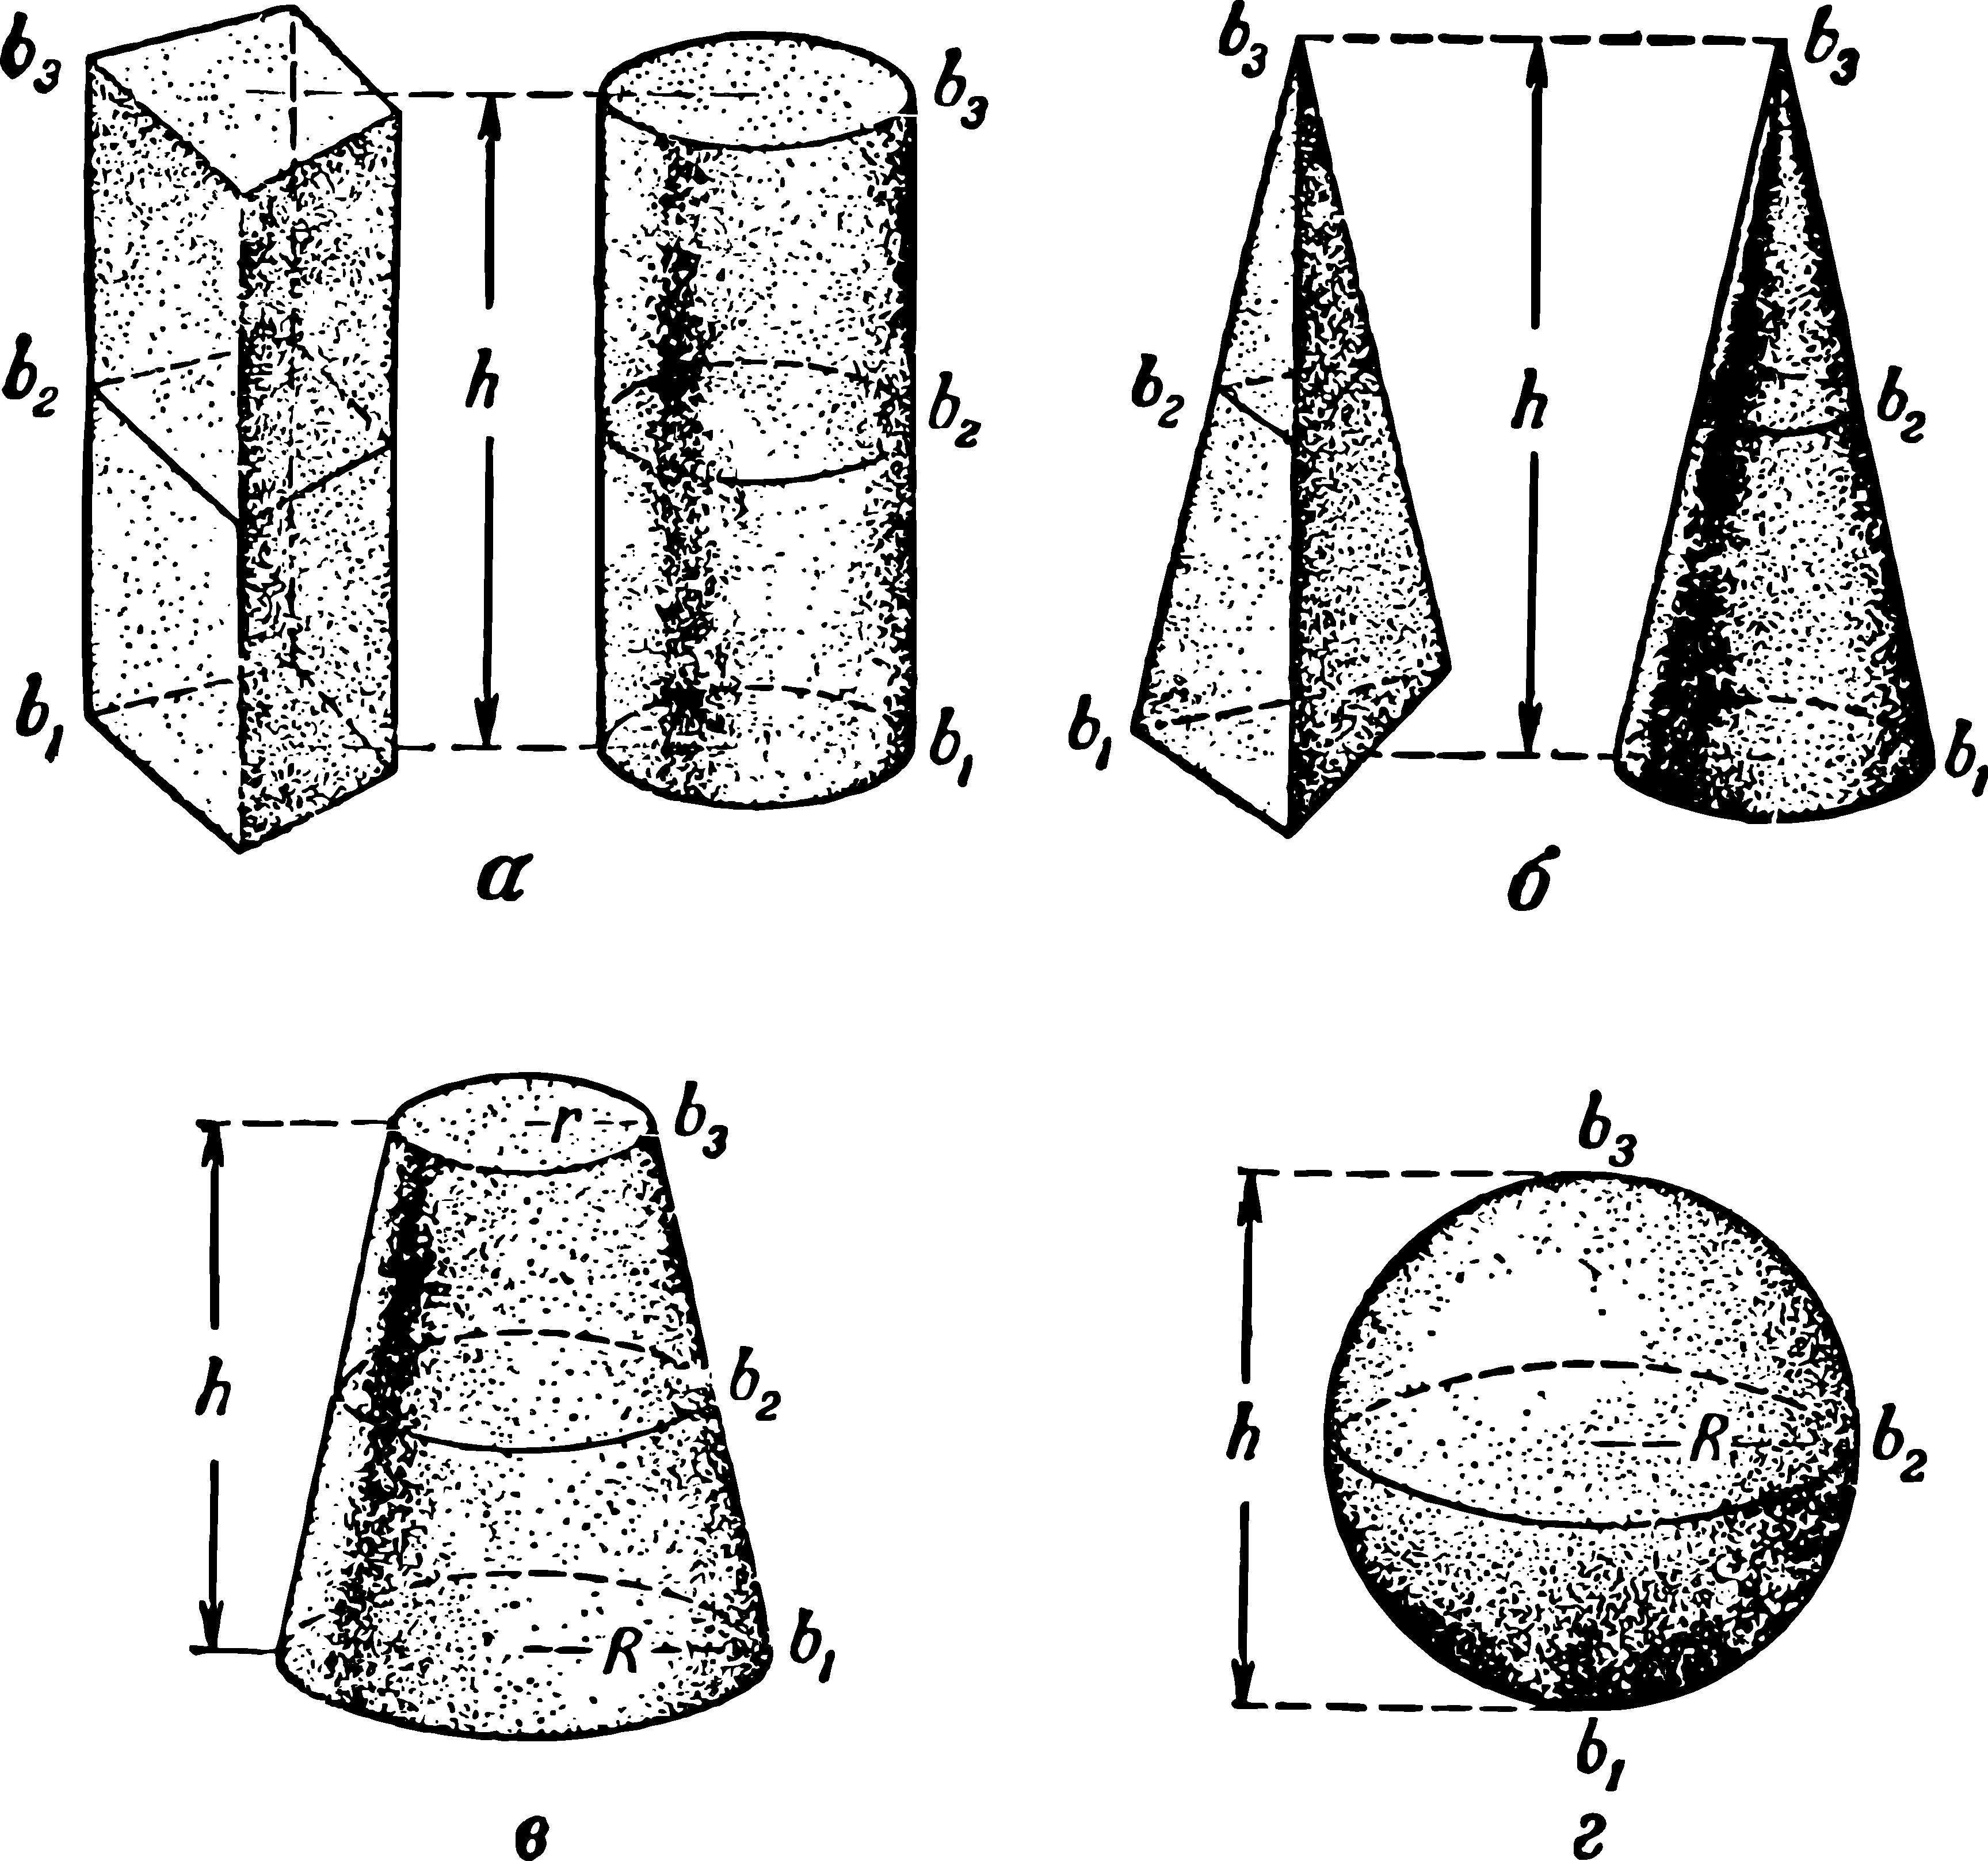
\includegraphics[width=0.9\textwidth]{figures/ch-01/fig-01-17.pdf}
\sidecaption[][-2cm]{Geometric bodies whose volumes can be calculated using a single formula.\label{fig-01-17}}
\end{figure}

\ques Let's note another interesting feature of our universal formula: it is also suitable for calculating the area of plane figures: parallelograms, trapezoids, and triangles, if by 
\begin{enumerate}[label=\textsection]
\item \( h \) we mean, as before, the height of the figure, 
\item by \( b_{1} \) the length of the lower base, 
\item by \( b_{2} \) the length of the middle base and 
\item by $b_{3}$ the length of the lower base. 
\end{enumerate}
How can we confirm this?

\ans Applying the formula, we have: for a parallelogram (square, rectangle) (see \figr{fig-01-18}~\drkgry{a})
\begin{equation*}%
S = \frac{h}{6}\, (b_{1} + 4 b_{1} + b_{1}) = b_{1}h;
\end{equation*}
for a trapezoid (see \figr{fig-01-18}~\drkgry{b})
\begin{equation*}%
S = \frac{h}{6}\, \left( b_{1} + 4 \frac{b_{1} + b_{2}}{2} + b_{3} \right) = \frac{h}{2}\,(b_{1} + b_{3});
\end{equation*}
for a triangle (see \figr{fig-01-18}~\drkgry{c})
\begin{equation*}%
S = \frac{h}{6}\, \left( b_{1} + 4 \frac{b_{1}}{2} + 0 \right) = \frac{b_{1}h}{2}.
\end{equation*}
You can see that our formula has enough right to be called universal.

\begin{figure}[h!]
\centering
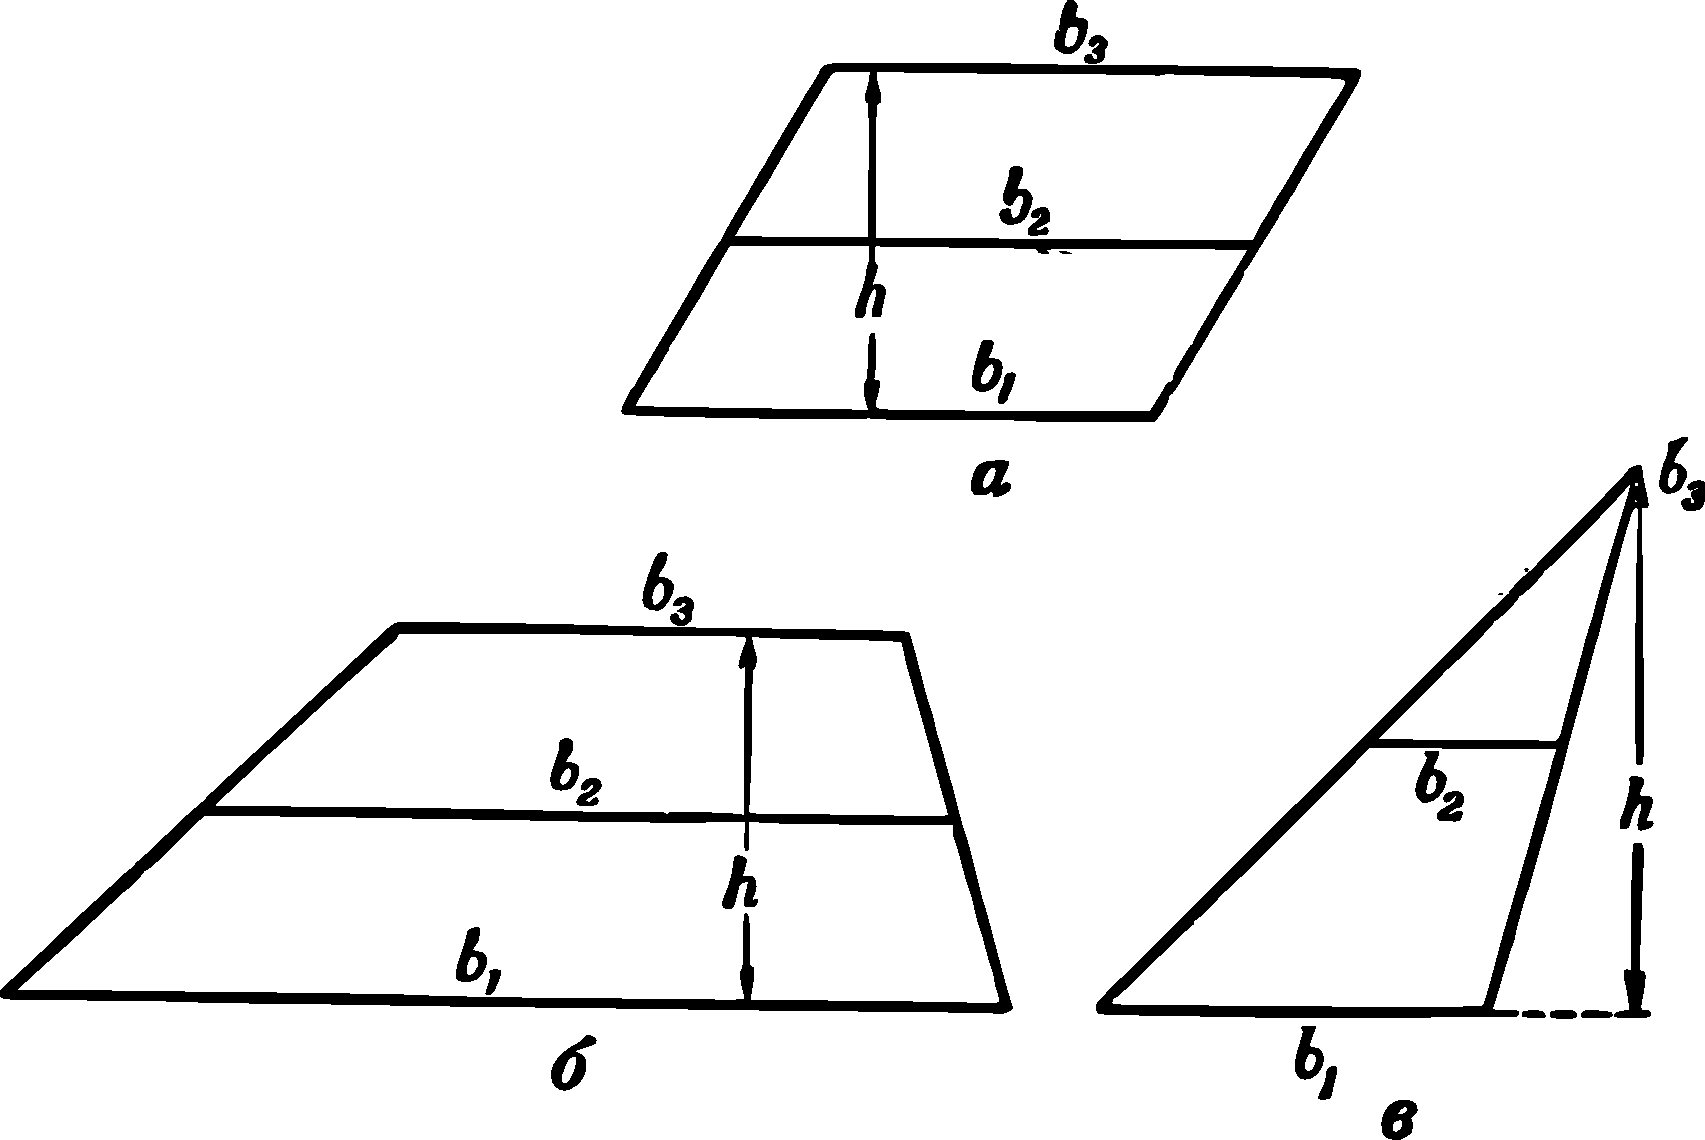
\includegraphics[width=\textwidth]{figures/ch-01/fig-01-18.pdf}
\sidecaption{The universal formula is also suitable for calculating the areas of these figures.\label{fig-01-18}}
\end{figure}


\section{Volume and Weight of a Tree at the Root}
\label{sec-1.12}

So, you have a formula with which you can approximately calculate the volume of a felled tree trunk without worrying about what geometric shape it resembles: a cylinder, a complete cone, or a truncated cone. For this, four measurements are needed -- the length of the trunk and three diameters: the lower cut, the upper, and in the middle of the length. Measuring the lower and upper diameters is very simple; however, determining the average diameter without a special device (``measuring fork'' used by foresters, see \figr{fig-01-19} and \figr{fig-01-20}\sidenote{A similar principle is applied in the well-known device for measuring the diameter of round objects -- the caliper \figr{fig-01-20}, to the right).} is quite difficult. But the difficulty can be overcome by encircling the trunk with a rope and dividing its length by 3 1/7 to get the diameter.

\begin{figure}[h!]
\centering
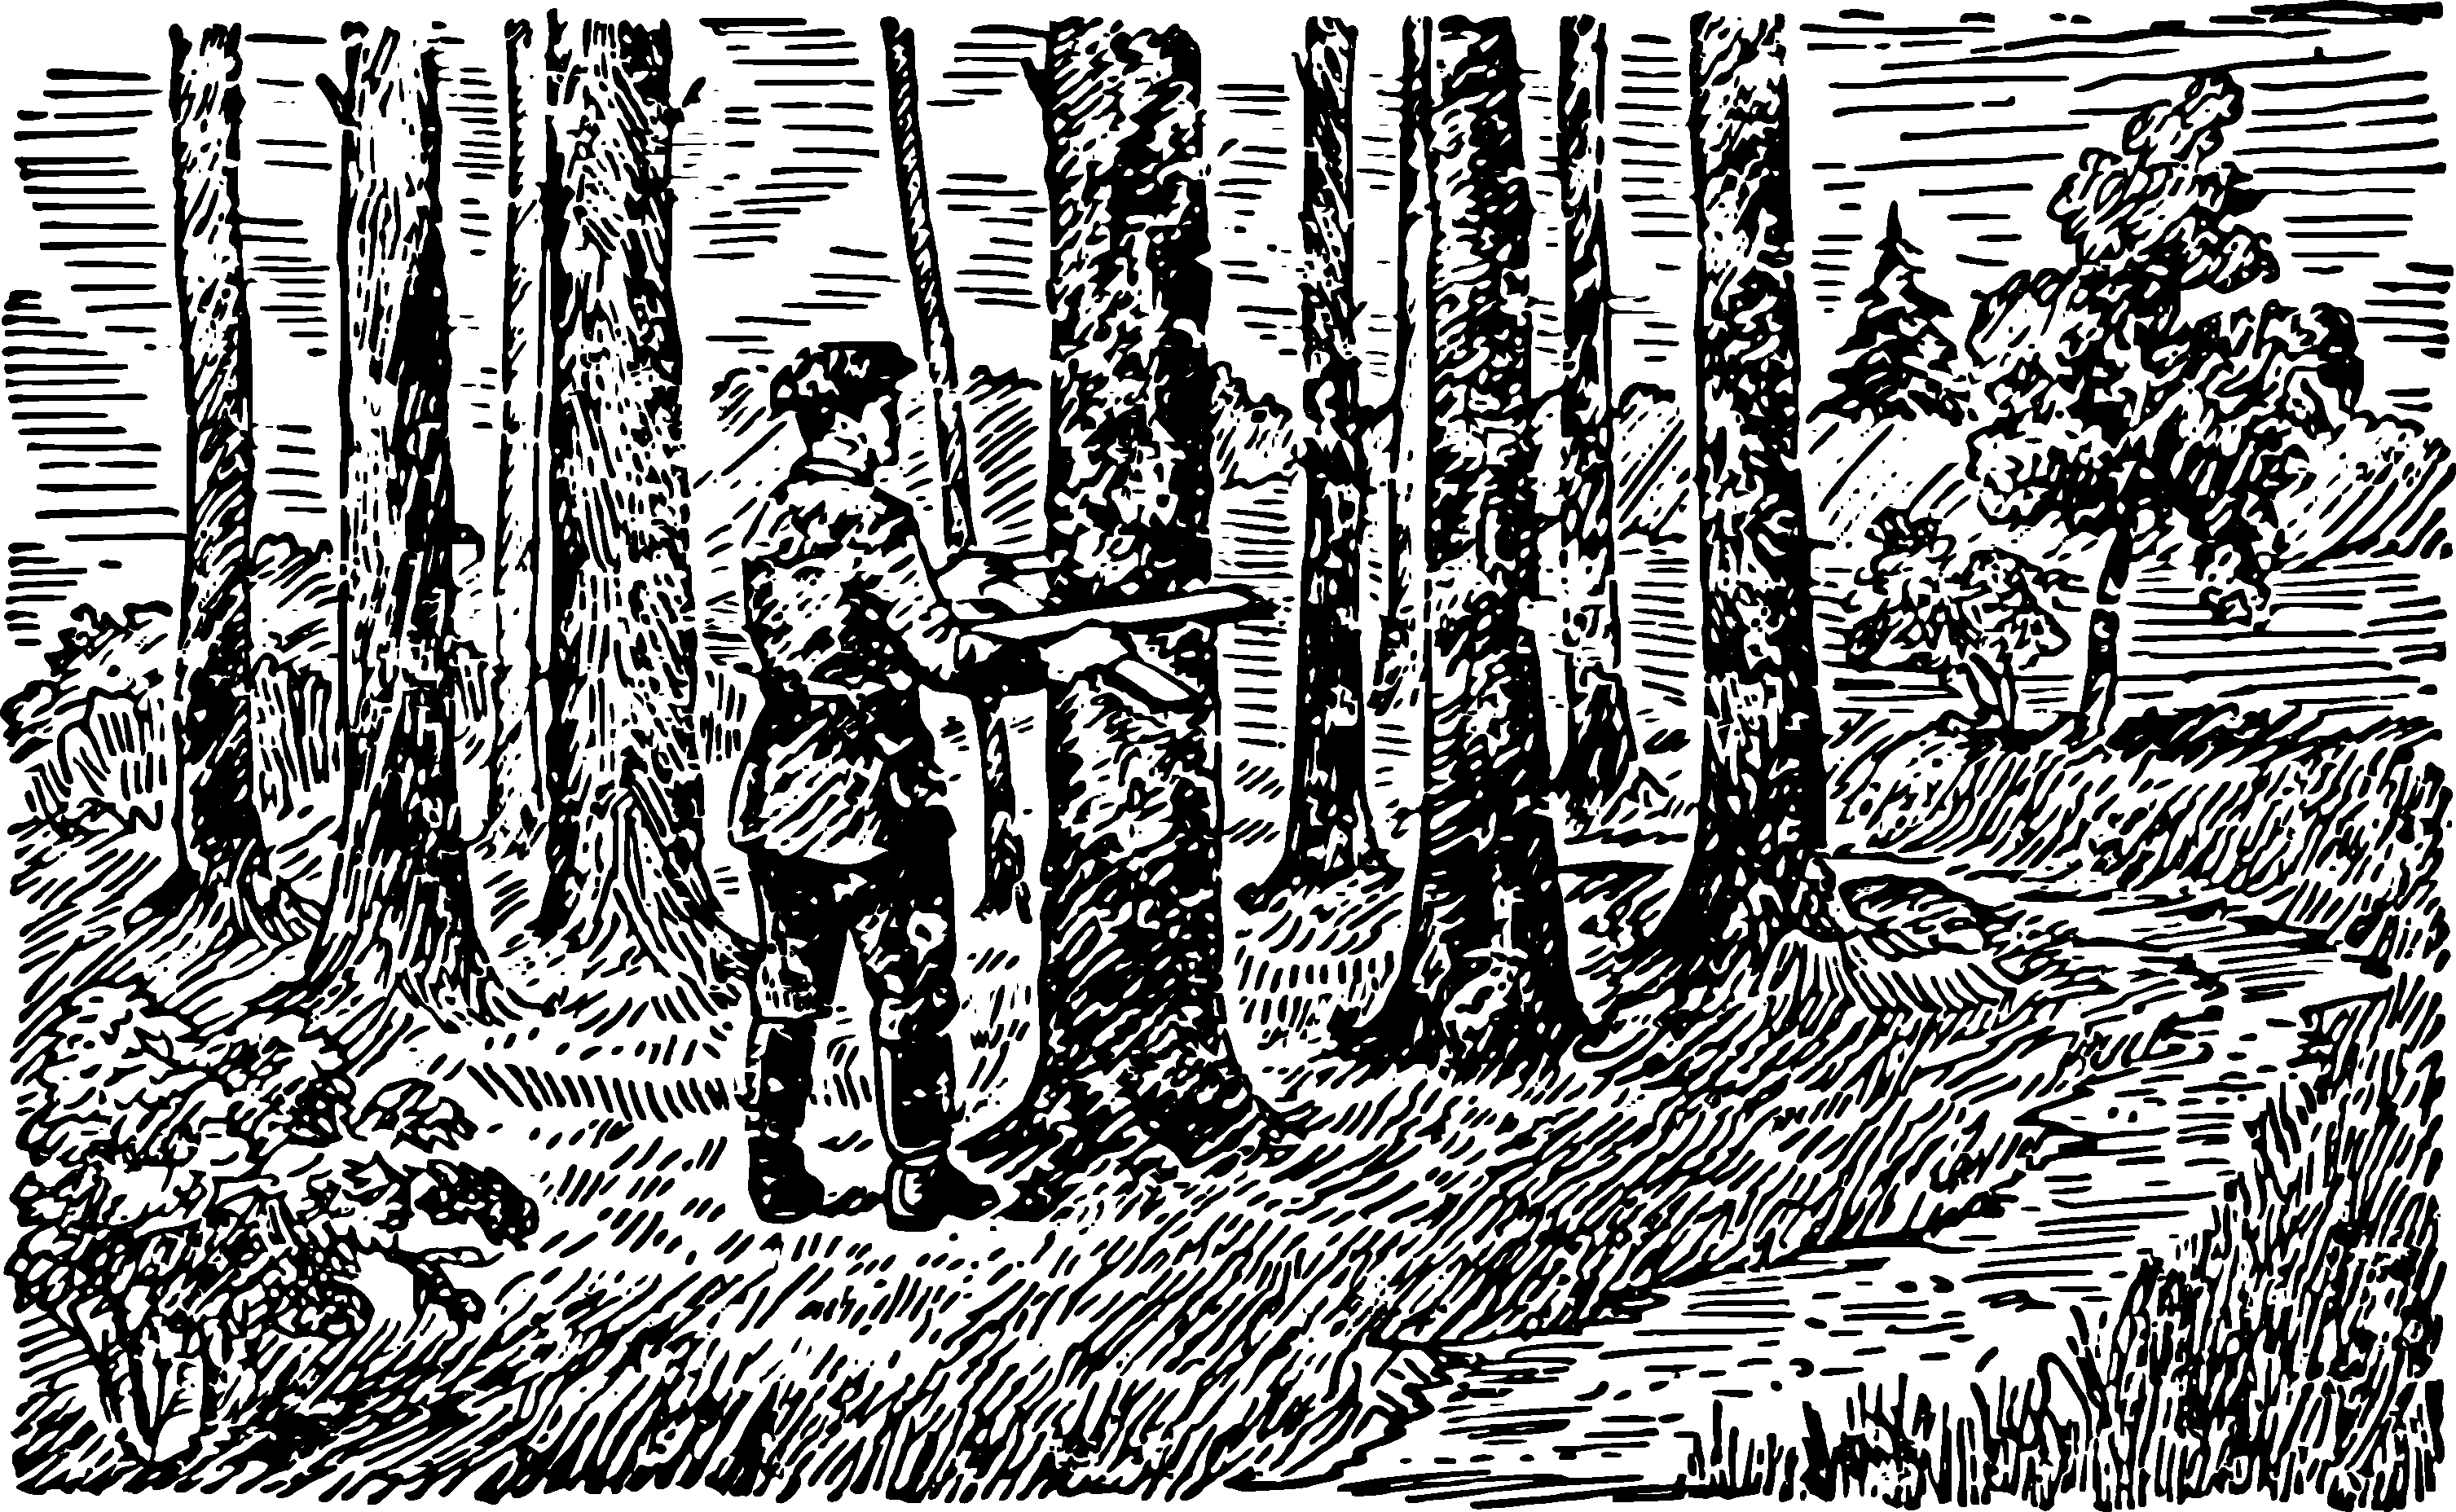
\includegraphics[width=\textwidth]{figures/ch-01/fig-01-19.pdf}
\sidecaption{Measuring the diameter of a tree with a measuring fork.\label{fig-01-19}}
\end{figure}


The volume of a felled tree trunk obtained in this way is accurate enough for many practical purposes. In short, but less accurately, this problem can be solved by calculating the volume of the trunk as the volume of a cylinder, the diameter of the base of which is equal to the diameter of the trunk in the middle of its length; however, the result obtained is underestimated, sometimes by 12\%. But if you mentally divide the trunk into two-meter segments and determine the volume of each of these almost cylindrical parts to then add them up, the result will be much better: it errs on the side of underestimation by no more than 2–3\%.

\begin{figure}[h!]
\centering
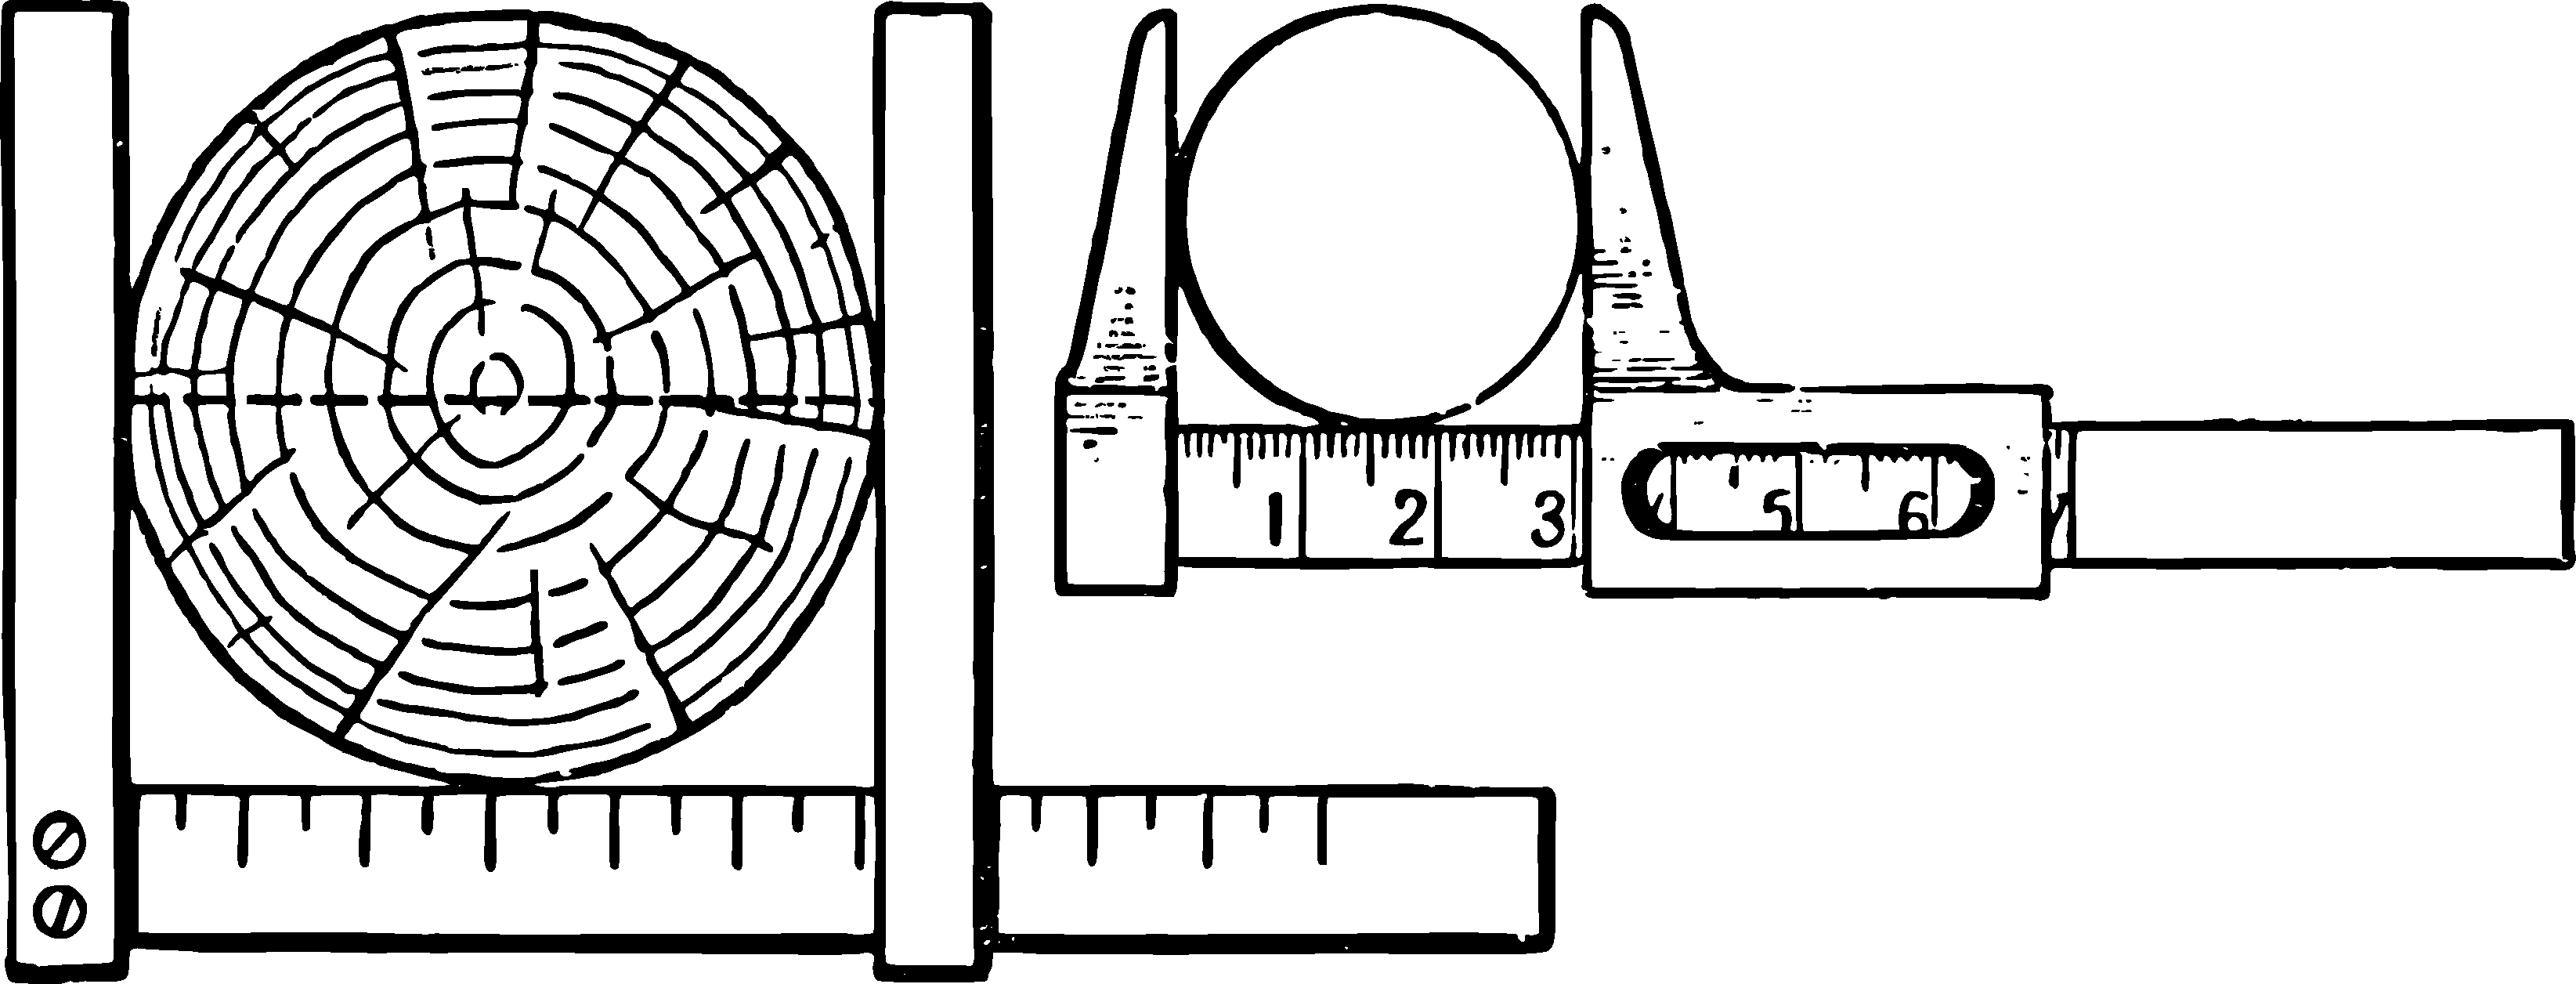
\includegraphics[width=0.9\textwidth]{figures/ch-01/fig-01-20.pdf}
\sidecaption{Measuring fork (left) and caliper (right).\label{fig-01-20}}
\end{figure}

However, all this is completely inapplicable to a tree at the root: if you are not going to climb it, then you can only measure the diameter of its lower part. In this case, to determine the volume, you will have to be satisfied with only a very approximate estimate, comforting yourself with the fact that professional foresters usually proceed in a similar way. They also use a table of so-called ``species numbers,'' i.e., numbers that show what proportion of the volume of the measured tree is compared to the volume of a cylinder of the same height and diameter, measured at the height of a grown man's chest, i.e., 130 cm (this height is the most convenient for measuring). 

\figr{fig-01-21} illustrates this clearly. Of course, ``species numbers'' vary for trees of different species and heights, as the shape of the trunk is variable. However, the fluctuations are not particularly great: for pine and fir trunks (grown in dense plantations), ``species numbers'' range from 0.45 to 0.51, i.e., are approximately half.

\begin{figure}[h!]
\centering
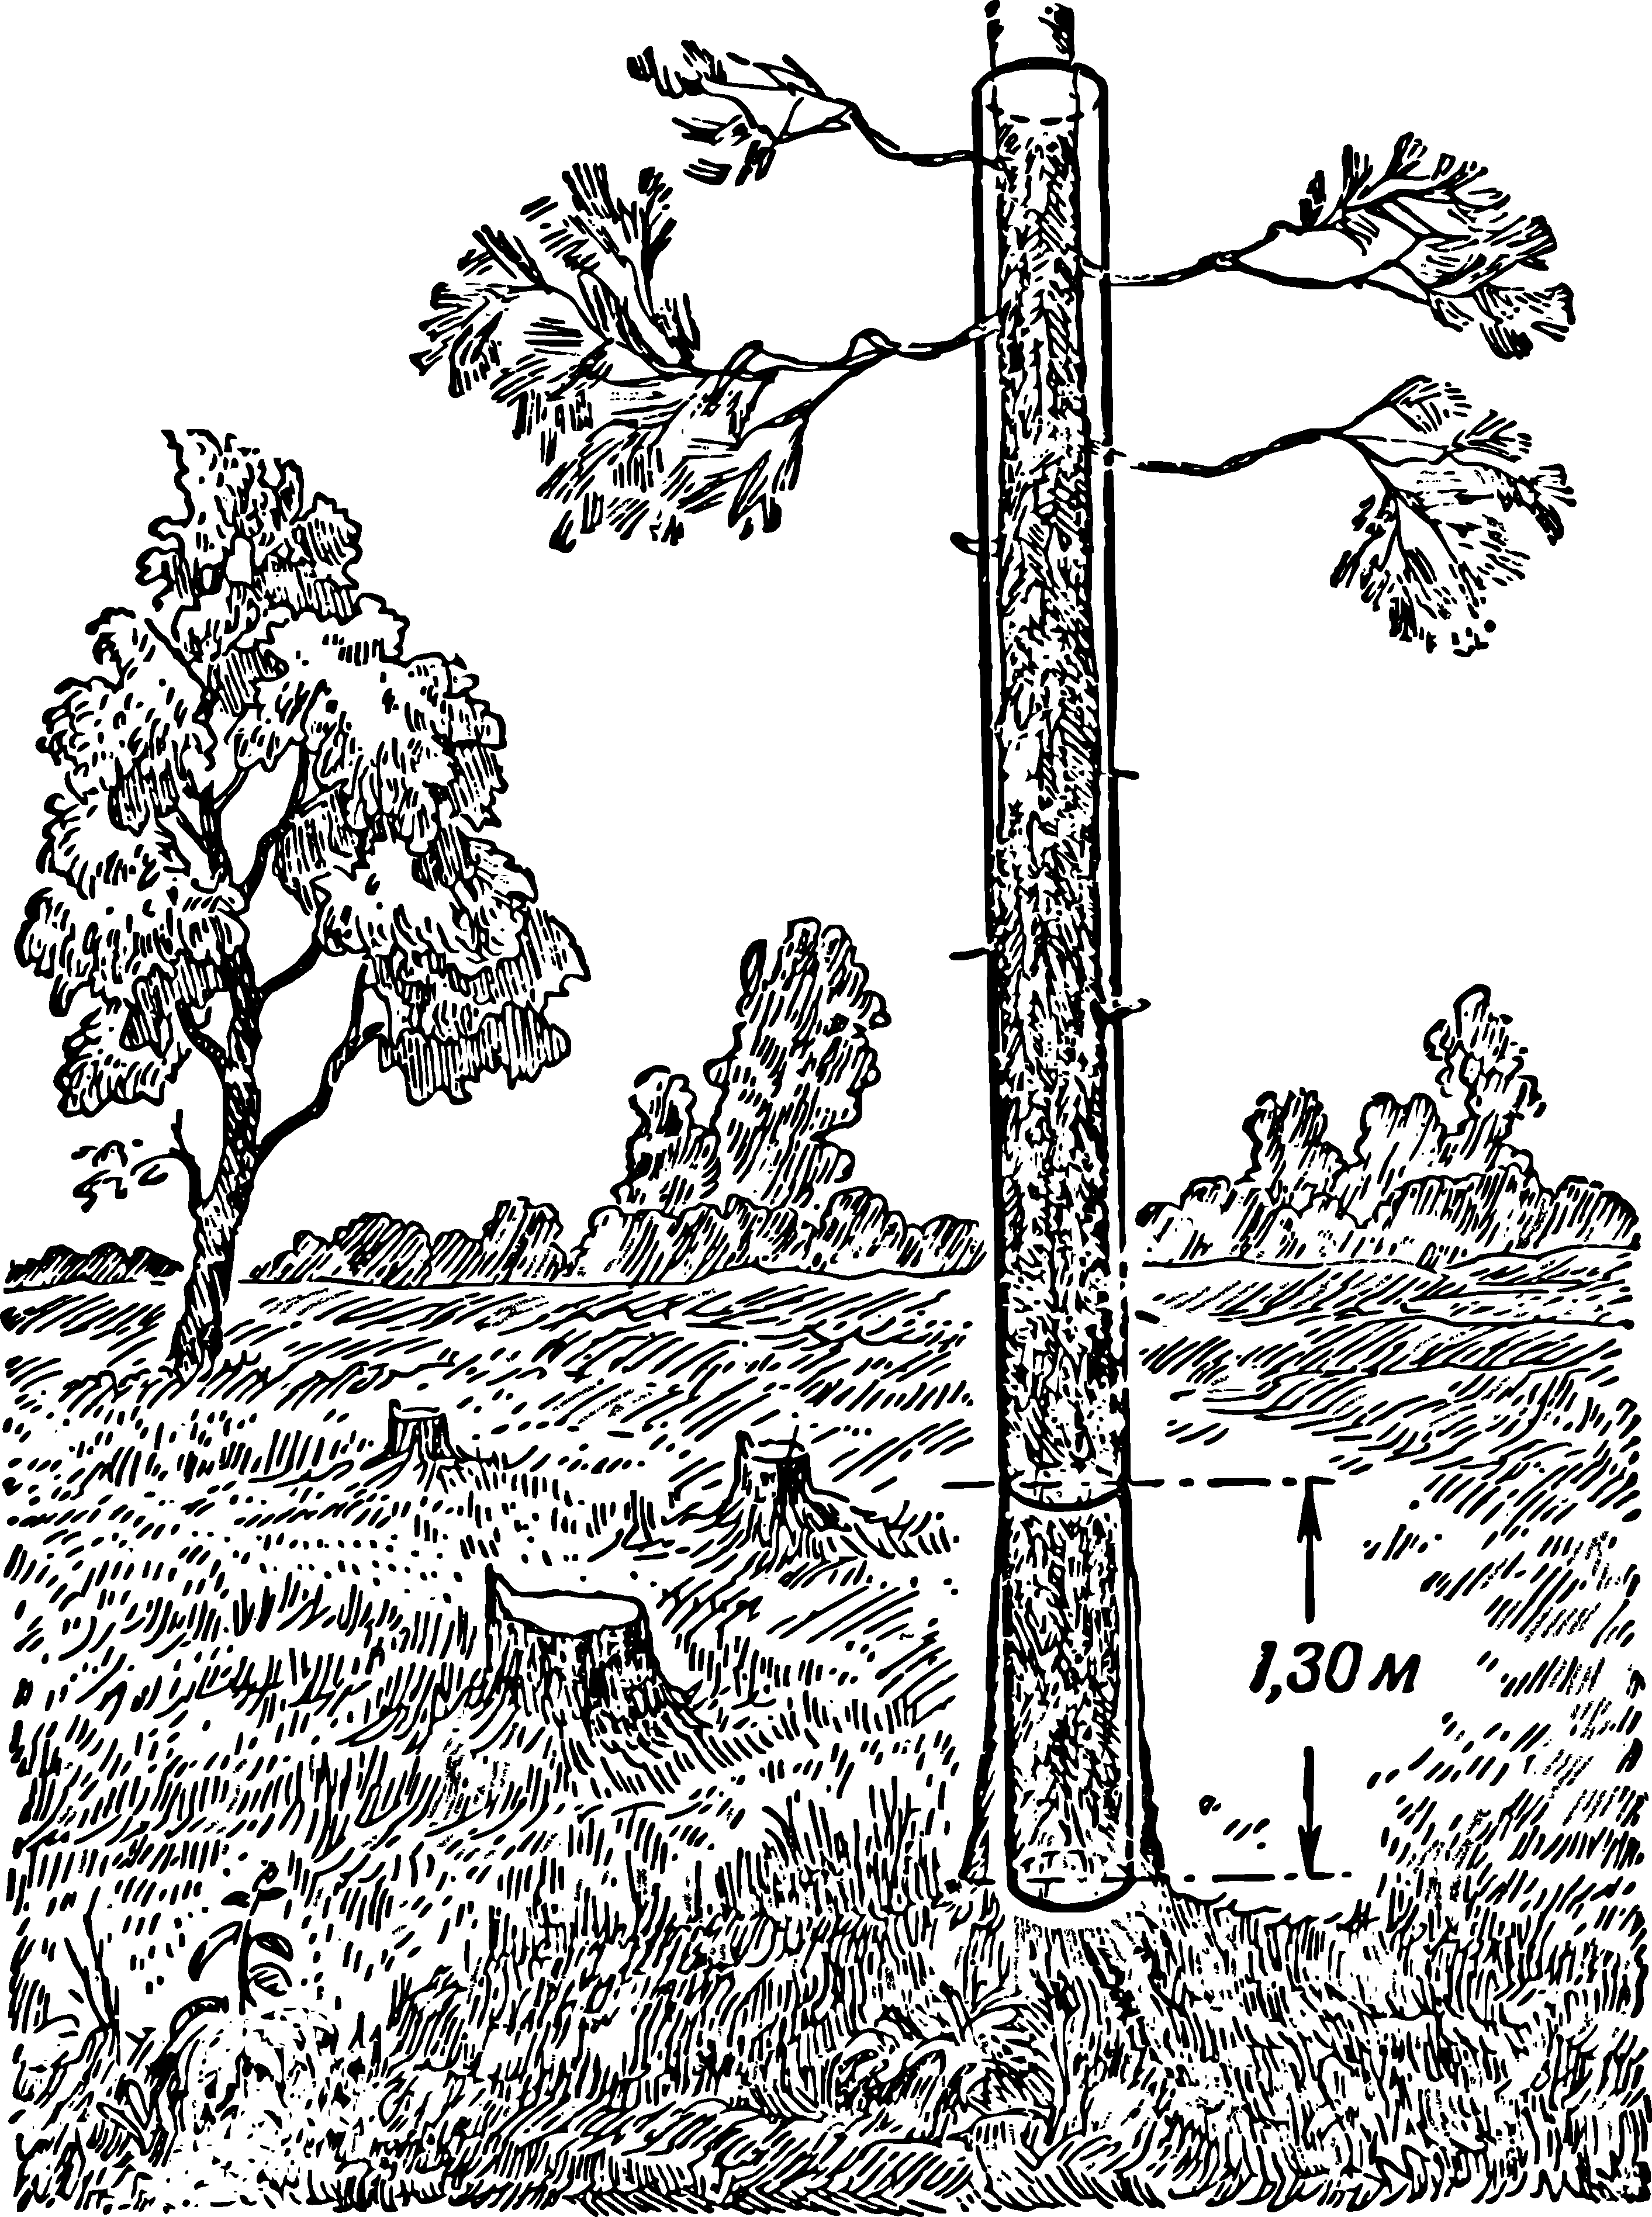
\includegraphics[width=0.8\textwidth]{figures/ch-01/fig-01-21.pdf}
\sidecaption[][-4cm]{What is a ``species number''?\label{fig-01-21}}
\end{figure}

Thus, without much error, it can be assumed that the volume of a coniferous tree at the root is half the volume of a cylinder of the same height with a diameter equal to the diameter of the tree at chest height.

This is, of course, only an approximate estimate, but it is not too far from the true result: up to 2\% in the overestimation direction and up to 10\% in the underestimation direction.\sidenote[][-1cm]{It must be remembered that ``species numbers'' refer only to trees that have grown in the forest, i.e. to tall and thin (smooth, without nodes); for free-standing branched trees, such general rules for calculating volume cannot be specified.}

From here, it is only one step towards estimating the weight of the tree at the root. For this, it is enough to know that 1 cubic meter of fresh pine or fir wood weighs about 600–700 kg. For example, suppose you are standing next to a fir tree, the height of which you have determined to be \SI{28}{\meter}, and the circumference of the trunk at chest height is \SI{120}{\centi\meter}. Then the area of the corresponding circle is \SI{1100}{\centi\meter\squared}, or \SI{0.11}{\meter\squared}, and the volume of the trunk is $1/2 \times 0.11 \times 28 = \SI{1.5}{\meter\cubed}$. Assuming that 1 cubic meter of fresh fir wood weighs on average \SI{650}{\kilo\gram}, we find that 1.0 cubic meter should weigh about a ton (\SI{1000}{\kilo\gram}).


\section{Leaf Geometry}
\label{sec-1.12}

\ques In the shadow of a silver poplar from its roots, a thicket has grown. Pick a leaf and notice how large it is compared to the leaves of the parent tree, especially those that grew in bright sunlight. The shaded leaves compensate for the lack of light with the size of their area, capturing sunlight rays. Understanding this is the task of botany. But the geometer can also have a say here: he can determine exactly how many times the area of the thicket leaf is larger than the area of the parent tree leaf.

How would you solve this problem?


\ans You can go two ways. First, determine the area of each leaf separately and find their ratio. The area of the leaf can be measured by covering it with transparent grid paper, each square of which corresponds, for example, to 4 square millimeters (a sheet of transparent grid paper used for this purpose is called a pallet). This is a perfectly correct but overly laborious method.\sidenote{However, this method has an advantage: using it, you can compare the areas of leaves with different shapes, which cannot be done according to the method described below.}

A shorter method is based on the fact that both leaves, different in size, still have the same or almost the same shape: in other words, they are geometrically similar figures. We know that the areas of such figures are related as the squares of their linear dimensions. Therefore, by determining how many times one leaf is longer or wider than the other, we can find the ratio of their areas simply by squaring this number. Let the thicket leaf be 15 cm long, and the leaf from the tree branch only 4 cm long; the ratio of their linear dimensions is 15/4, and therefore, in terms of area, one is larger than the other by 225/16 times, or about 14. Rounding off (since full accuracy cannot be achieved here), we can say that the thicket leaf is approximately 15 times larger than the tree leaf in terms of area.

Let us consider another example.
%\clearpage

\ques At a dandelion grown in shade, a leaf is 31 cm long. At another specimen grown in sunlight, the leaf blade is only 3.3 cm long. Approximately how many times is the area of the first leaf larger than the area of the second?



\ans We proceed as before. The ratio of the areas is
\begin{equation*}%
\frac{31^{2}}{3.3^{2}} = \frac{960}{10.9} = 87;
\end{equation*}
so one leaf is approximately 90 times larger than the other in terms of area.

\begin{marginfigure}[-3.5cm]%[h!]
\centering
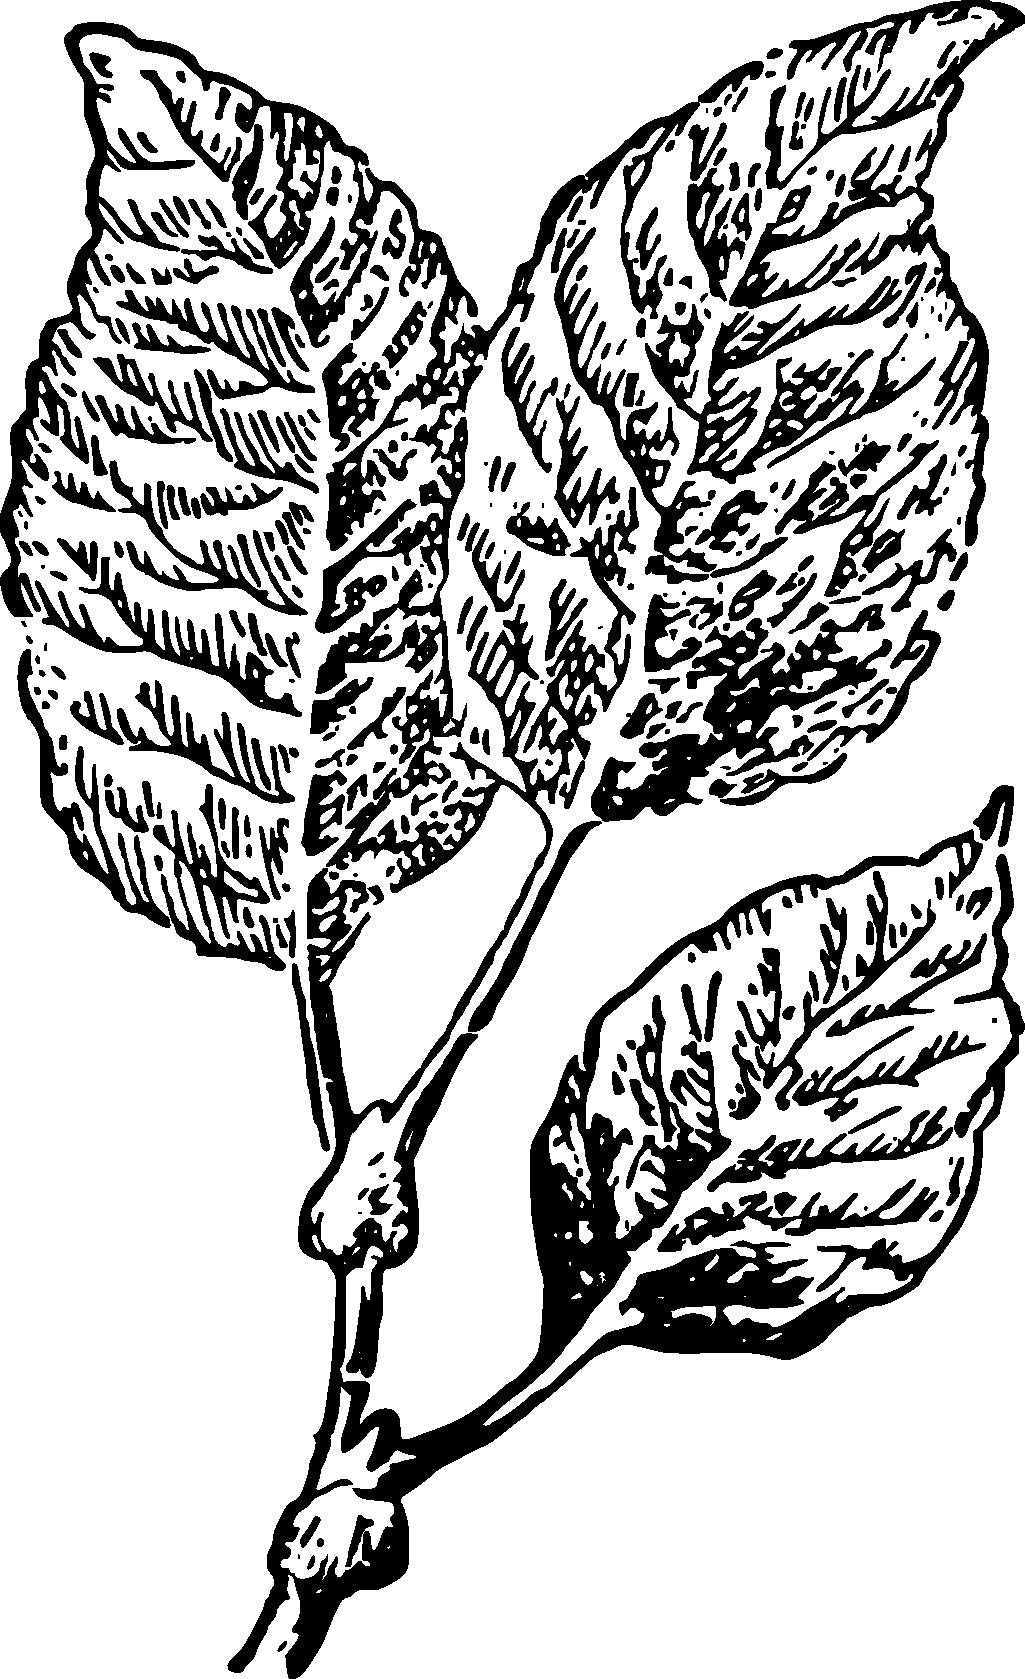
\includegraphics[width=0.9\textwidth]{figures/ch-01/fig-01-22.pdf}
\sidecaption{Determine the ratio of the areas of these leaves.\label{fig-01-22}}
\end{marginfigure}


It is easy to find in the forest many pairs of leaves of the same shape but different sizes, thus providing interesting material for geometric problems on the ratio of areas of similar figures. It always seems strange to an unaccustomed eye that a relatively small difference in the length and width of leaves results in a noticeable difference in their areas. For example, if two leaves, geometrically similar in shape, differ in length by 20\%, then the ratio of their areas is 
\begin{equation*}%
1.2^{2} \approx 1.4, 
\end{equation*}
meaning the difference is 40\%. And with a difference in width of 40\%, One leaf exceeds the other in area by 
\begin{equation*}%
1.4^{2} \approx 2, 
\end{equation*}
or nearly twice.

\ques  We invite the reader to determine the ratio of the areas of the leaves depicted in \figr{fig-01-22} and \figr{fig-01-23}.

\begin{marginfigure}[-4.5cm]%[h!]
\centering
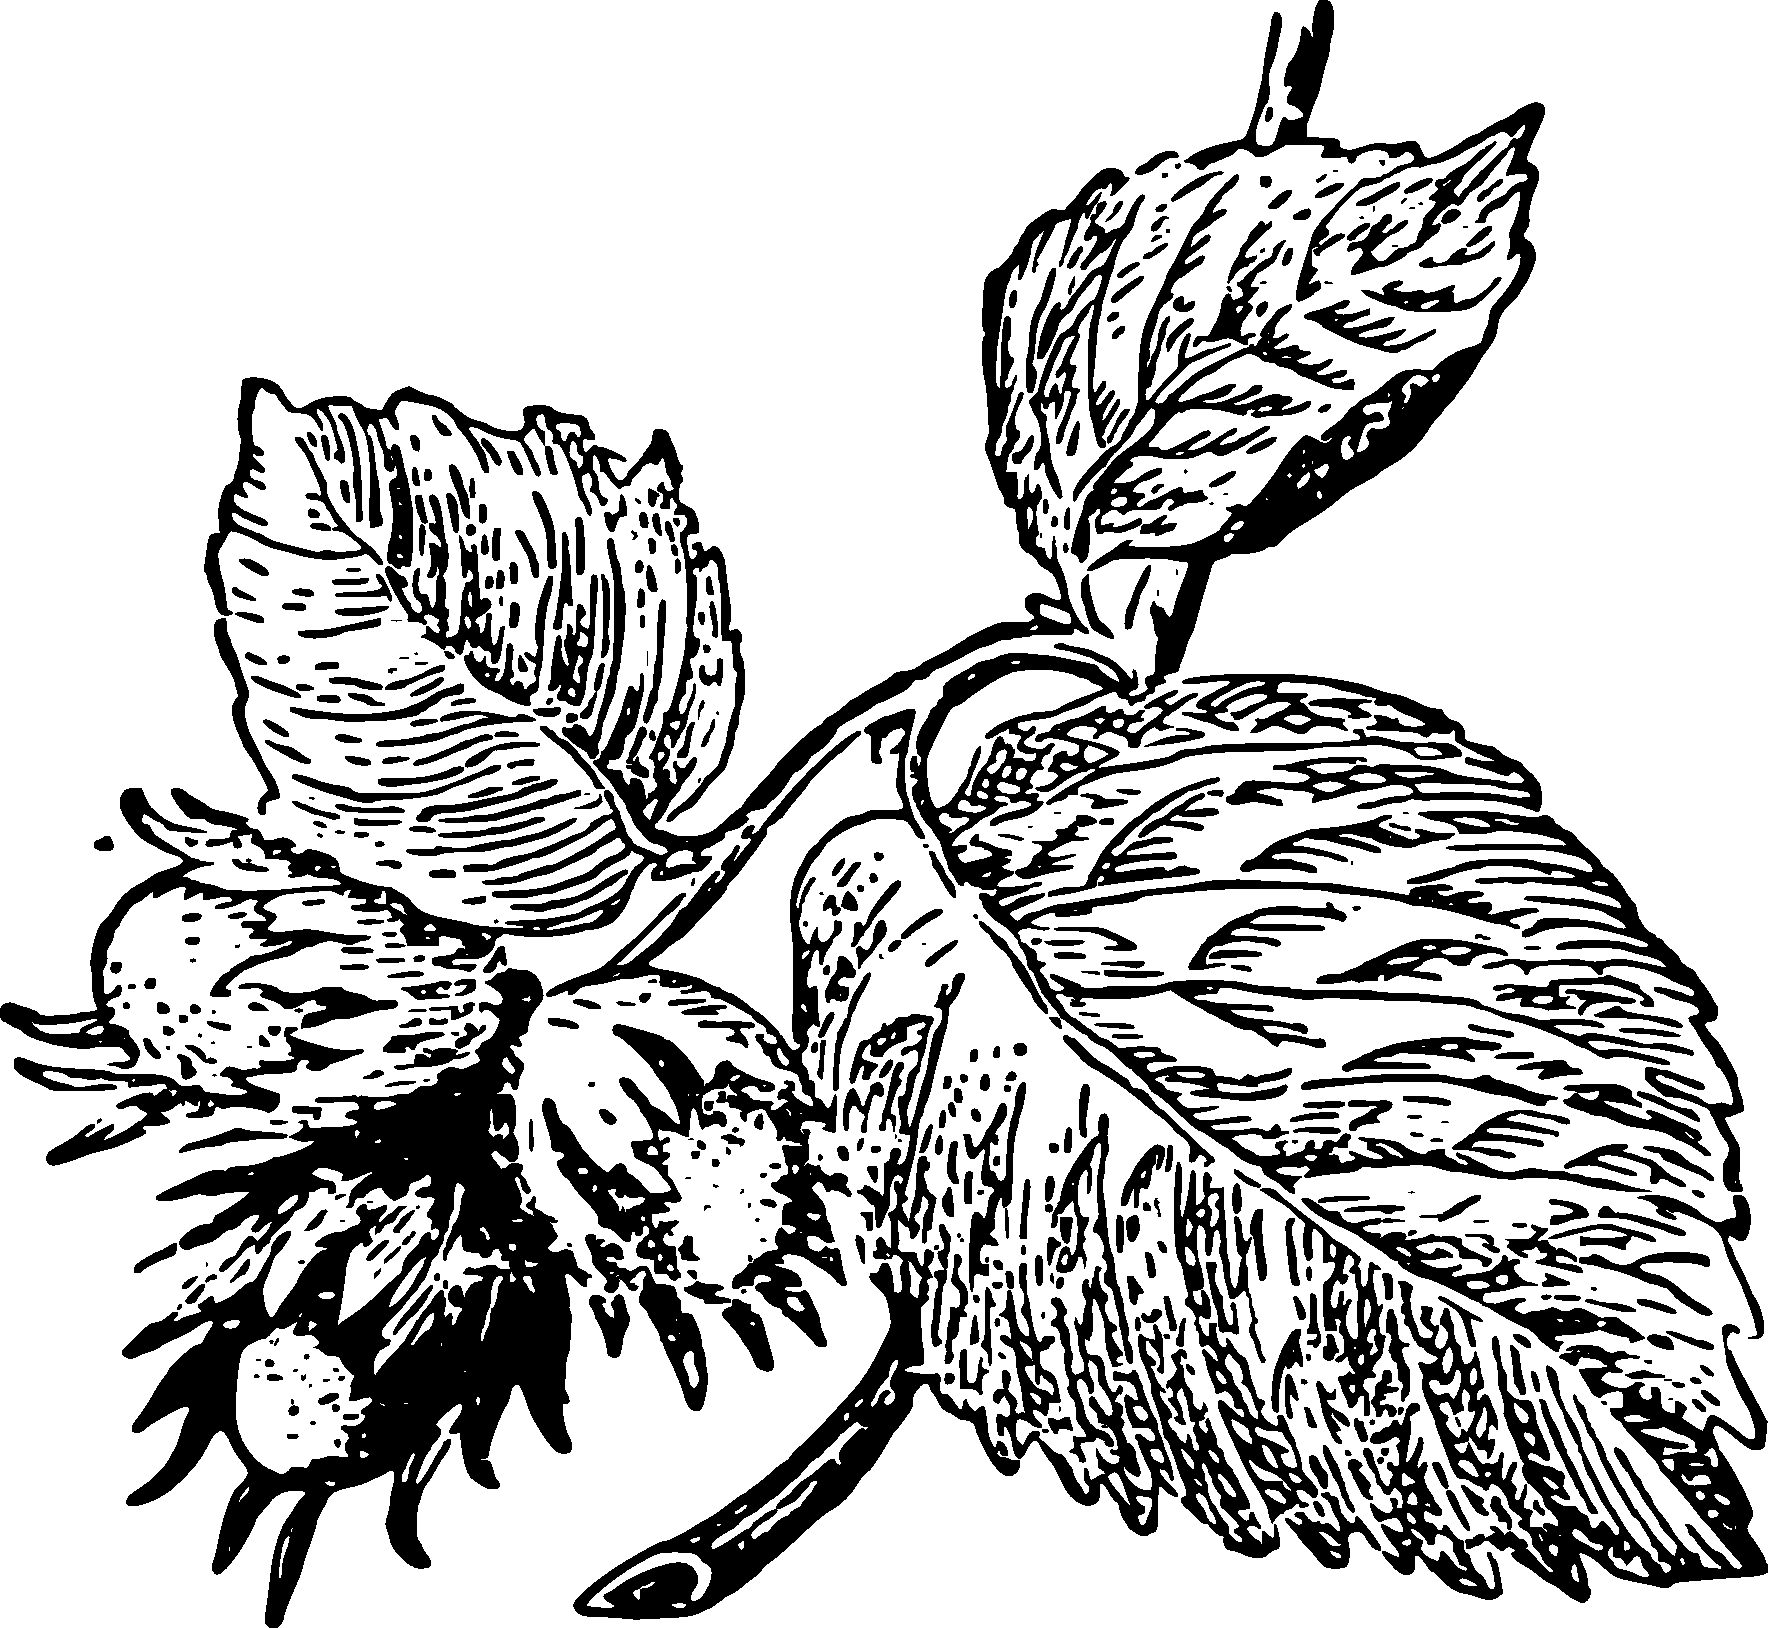
\includegraphics[width=0.9\textwidth]{figures/ch-01/fig-01-23.pdf}
\sidecaption{Determine the ratio of the areas of these leaves.\label{fig-01-23}}
\end{marginfigure}


%\ques \textsf{\small\color{Salmon} We invite the reader to determine the ratio of the areas of the leaves depicted in \figr{fig-01-22}and \figr{fig-01-23}.}

\section{Six-legged heroes}
\label{sec-1.14}

Amazing creatures, ants! Swiftly climbing up stems with a burden much heavier than their tiny size (\figr{fig-01-24}), ants present an intriguing puzzle to observant individuals: where does the insect derive the strength to effortlessly carry a load ten times its own weight? Indeed, a human might struggle to climb stairs while carrying, for instance, a piano (\figr{fig-01-24}), with the weight ratio of the load to the body being roughly similar to that of an ant. Thus, it seems that the ant is relatively stronger than a human!

But is it really so?

Without geometry, this cannot be understood. Let's listen to what the expert (Professor A.F. Brandt) has to say, primarily about the strength of muscles, and then about the current question regarding the comparison of forces between the insect and the human: ``A muscle resembles a resilient cord; however, its contraction is based not on elasticity, but on other reasons, and is normally manifested under the influence of nervous excitation, as demonstrated in physiological experiments involving the application of electric current to the corresponding nerve or directly to the muscle.''

``These experiments are easily conducted on muscles excised from a freshly killed frog, as the muscles of cold-blooded animals retain their vital properties for a long time even outside the organism, even at ordinary temperatures. The experiment is very simple. The main calf muscle, which extends the hind leg, is excised together with a piece of the femur bone from which it originates, and together with the terminal tendon. This muscle is found to be the most convenient due to its size, shape, and ease of preparation. A hook is passed through the tendon, and a weight is attached to it.'' 

\begin{marginfigure}[-3cm]%[h!]
\centering
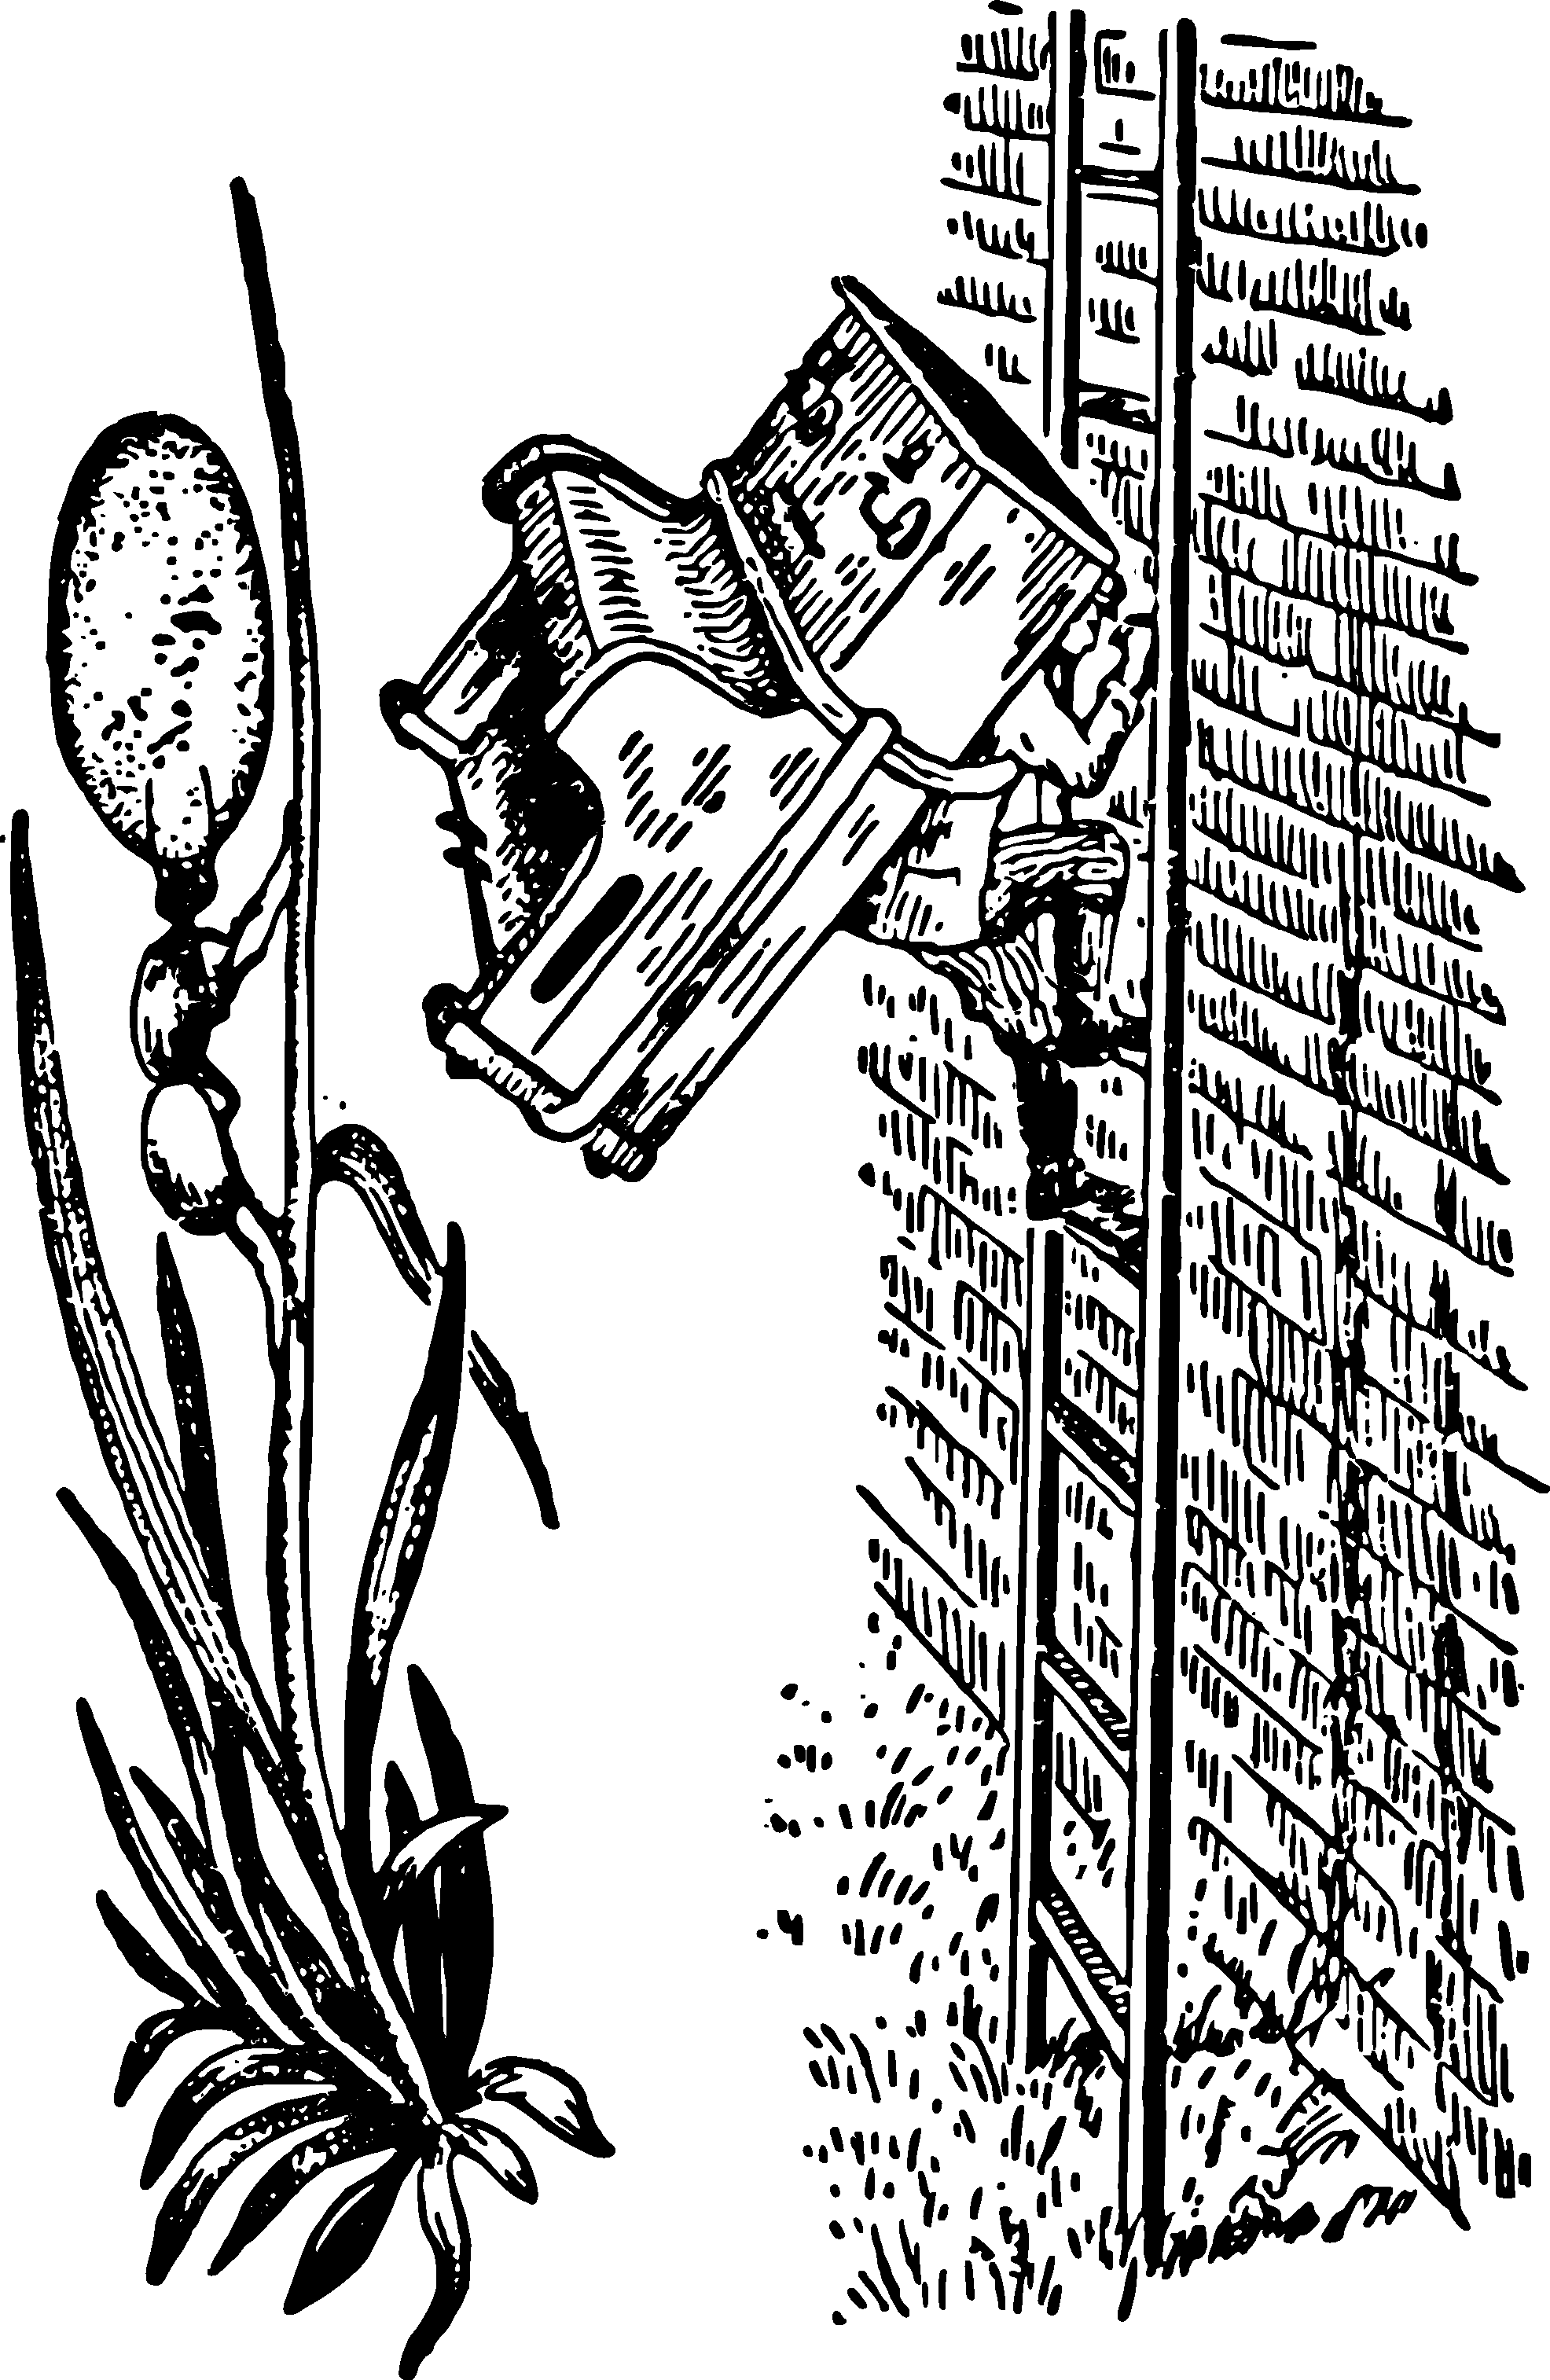
\includegraphics[width=\textwidth]{figures/ch-01/fig-01-24.pdf}
\sidecaption{The six-legged hero.\label{fig-01-24}}
\end{marginfigure}


``If wires from a galvanic element are touched to such a muscle, it instantly contracts, shortens, and lifts the load. By gradually adding additional weights, the maximum lifting capacity of the muscle can be easily determined. Now, if we bind together in length two, three, or four identical muscles and stimulate them simultaneously, we will not achieve greater lifting force; the load will only be lifted to a greater height, corresponding to the sum of the contractions of individual muscles. However, if we bundle two, three, or four muscles together, the entire system will lift a weight many times greater when stimulated. The same result, obviously, would be obtained if the muscles were fused together. Thus, we conclude that the lifting force of muscles depends not on their length or total mass, but only on their thickness, i.e., \emph{cross-sectional area}.''

``After this digression, let's turn to the comparison of similarly structured, geometrically similar, but differently sized animals. Let's imagine two animals: the original and one that has been doubled in size in all linear dimensions. In the second animal, the volume and weight of the entire body, as well as each of its organs, will be eight times greater; however, all corresponding planar dimensions, including the cross-sectional area of muscles, will be only four times greater. It turns out that as the animal grows to twice the length and eight times the weight, its muscular strength increases only fourfold, i.e., the animal becomes relatively weaker. Based on this reasoning, an animal that is three times longer (with cross-sectional areas three times larger and a weight 27 times greater) would be relatively three times weaker, and one that is four times longer would be four times weaker, and so on.''

``The law of unequal growth in volume and weight of the animal, and thus of muscular strength, explains why insects -- as observed in ants, predatory wasps, and others -- can carry loads 30 to 40 times their own weight, whereas a human can typically carry excluding gymnasts and porters -- only about 9/10 times their own weight, -- and a horse, which we view as a magnificent living work machine, even less, namely, only about 7/10 of its own weight.''\sidenote{For more details, see \emph{Fun with Physics} by Ya. I. Perelman, Chapter X \emph{Mechanics in the Living World}.}

After these explanations, we will look at the feats of that ant-giant with different eyes, about whom I.A. Krylov mockingly wrote:
\begin{quote}
\emph{Some ant had extraordinary strength,\\
 Such as was unheard of even in ancient times; \\
 He even (says his faithful historian)\\
 Could lift two barley grains.}
\end{quote} 


\begin{center}
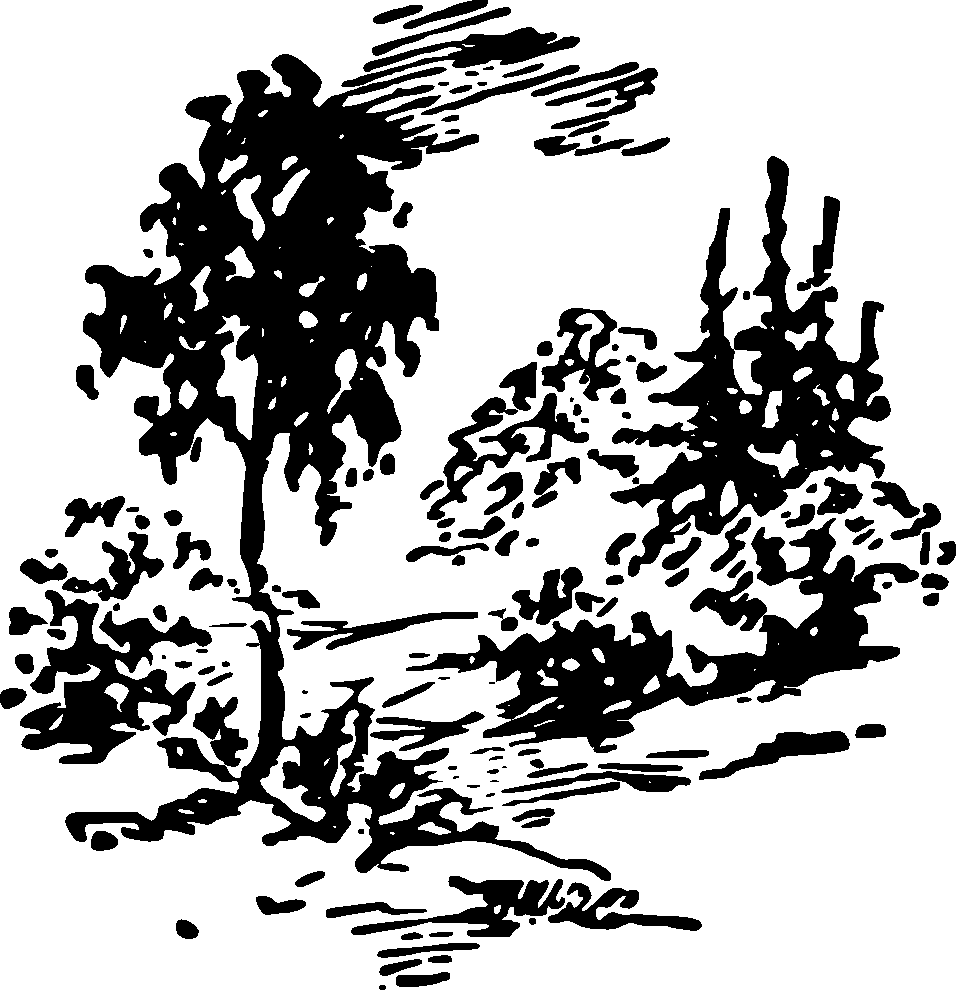
\includegraphics[width=0.3\textwidth]{figures/ch-01/fig-ch-01-tail.pdf}
\end{center}



















% !TEX root = perelman-geometry.tex
%!TEX TS-program = pdflatex
%!TEX encoding = UTF-8 Unicode

\setchapterpreamble[o]{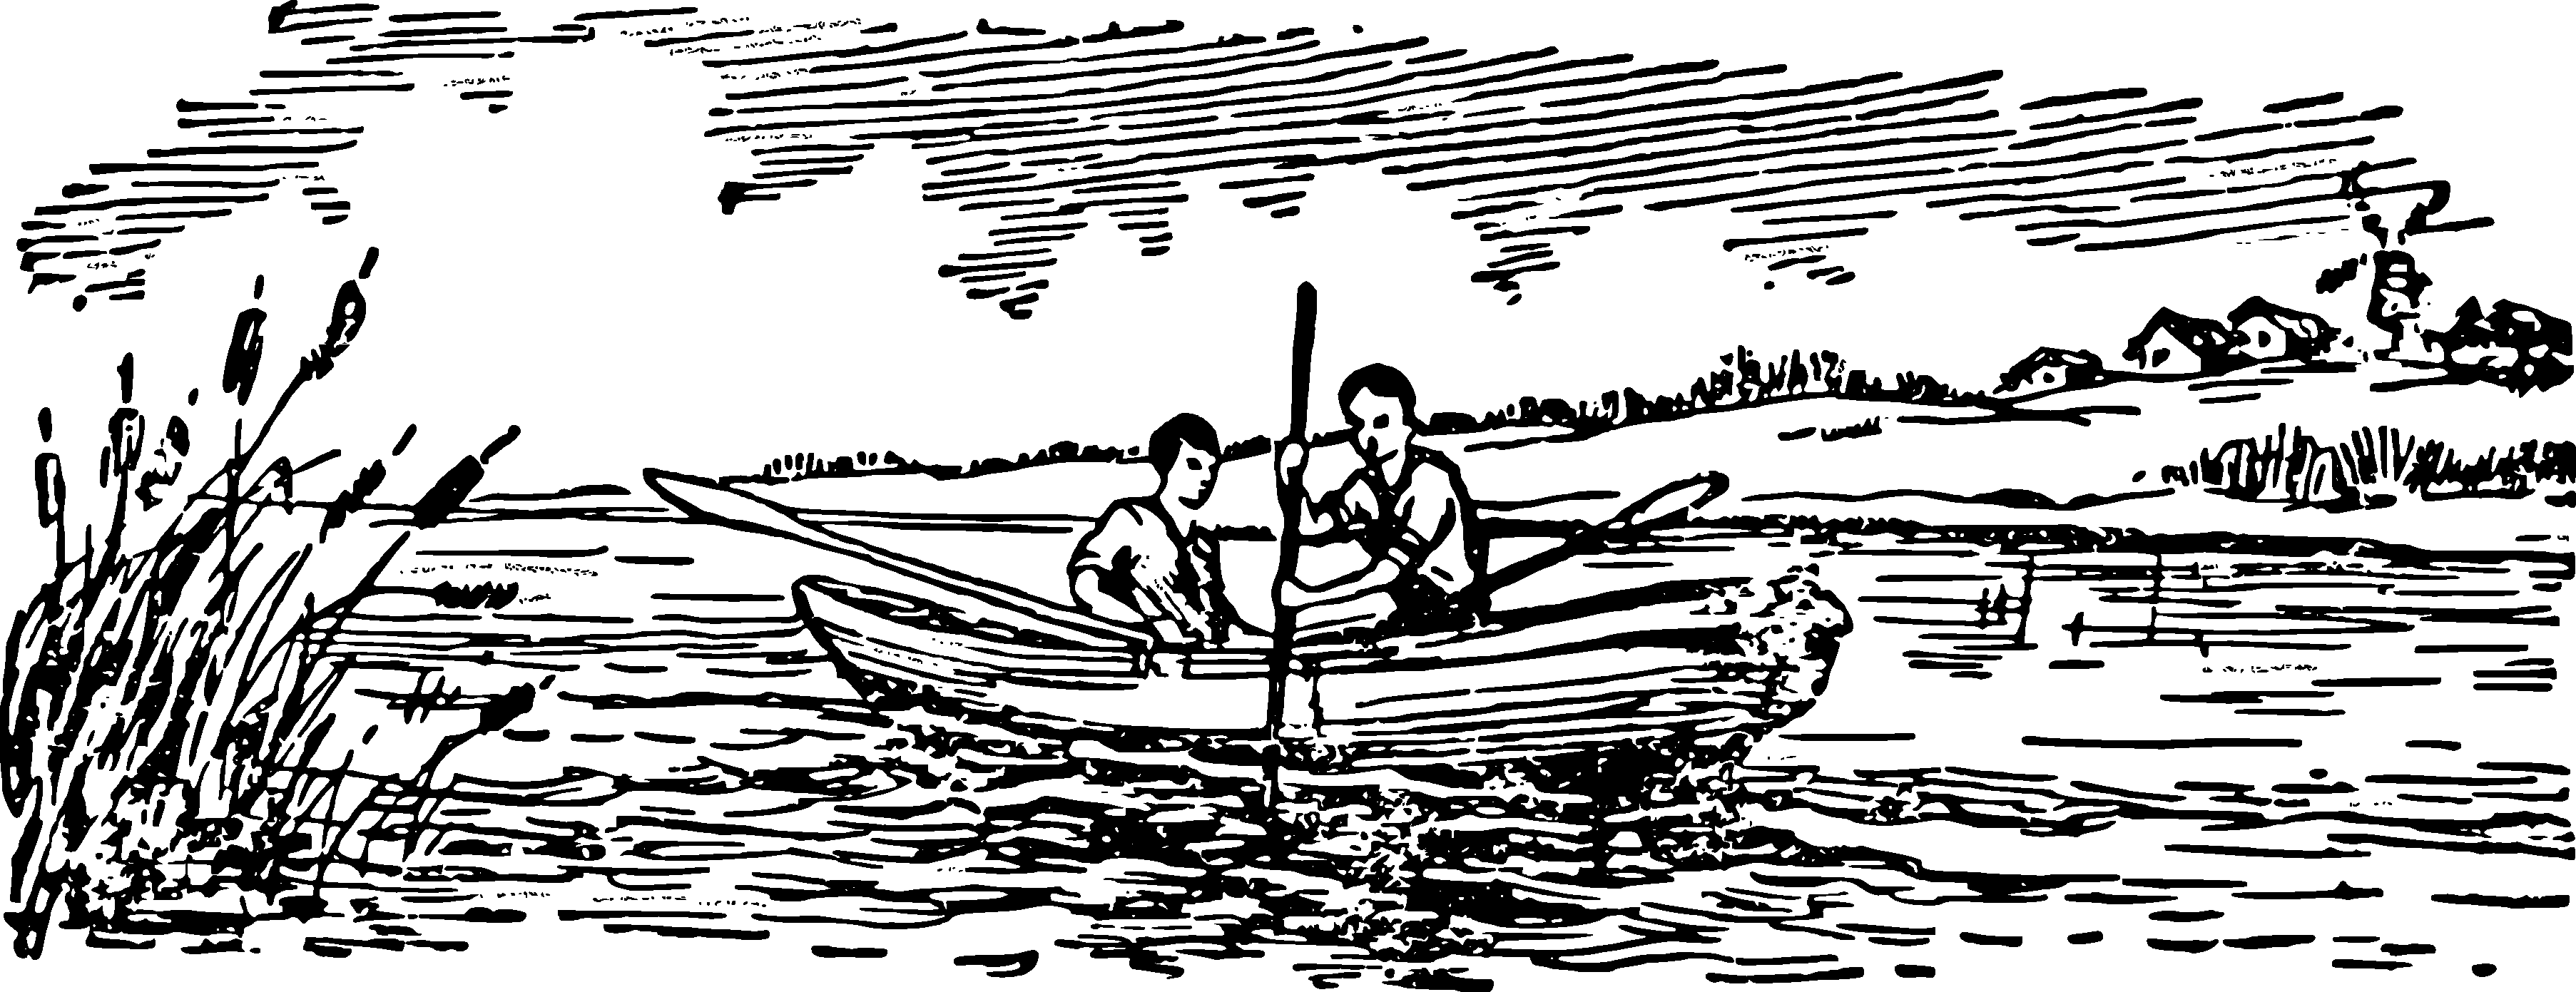
\includegraphics[width=1.2\textwidth]{figures/ch-02/fig-ch-02-head.pdf}\bigskip}

\chapter{Geometry By The River}
\label{ch-02}

\section{Measuring the width of the river}
\label{sec-2.1}
When crossing a river, measuring its width is just as easy for those who know geometry, how to determine the height of a tree, without climbing to the top. The inaccessible distance is measured the same techniques that we used to measure the inaccessible height. In both cases, the definition of the desired distance is replaced an example of another distance that is easily measurable directly.

Of the many ways to solve this problem, let's look at some of the simplest ones.

\begin{figure}[h!]
\centering
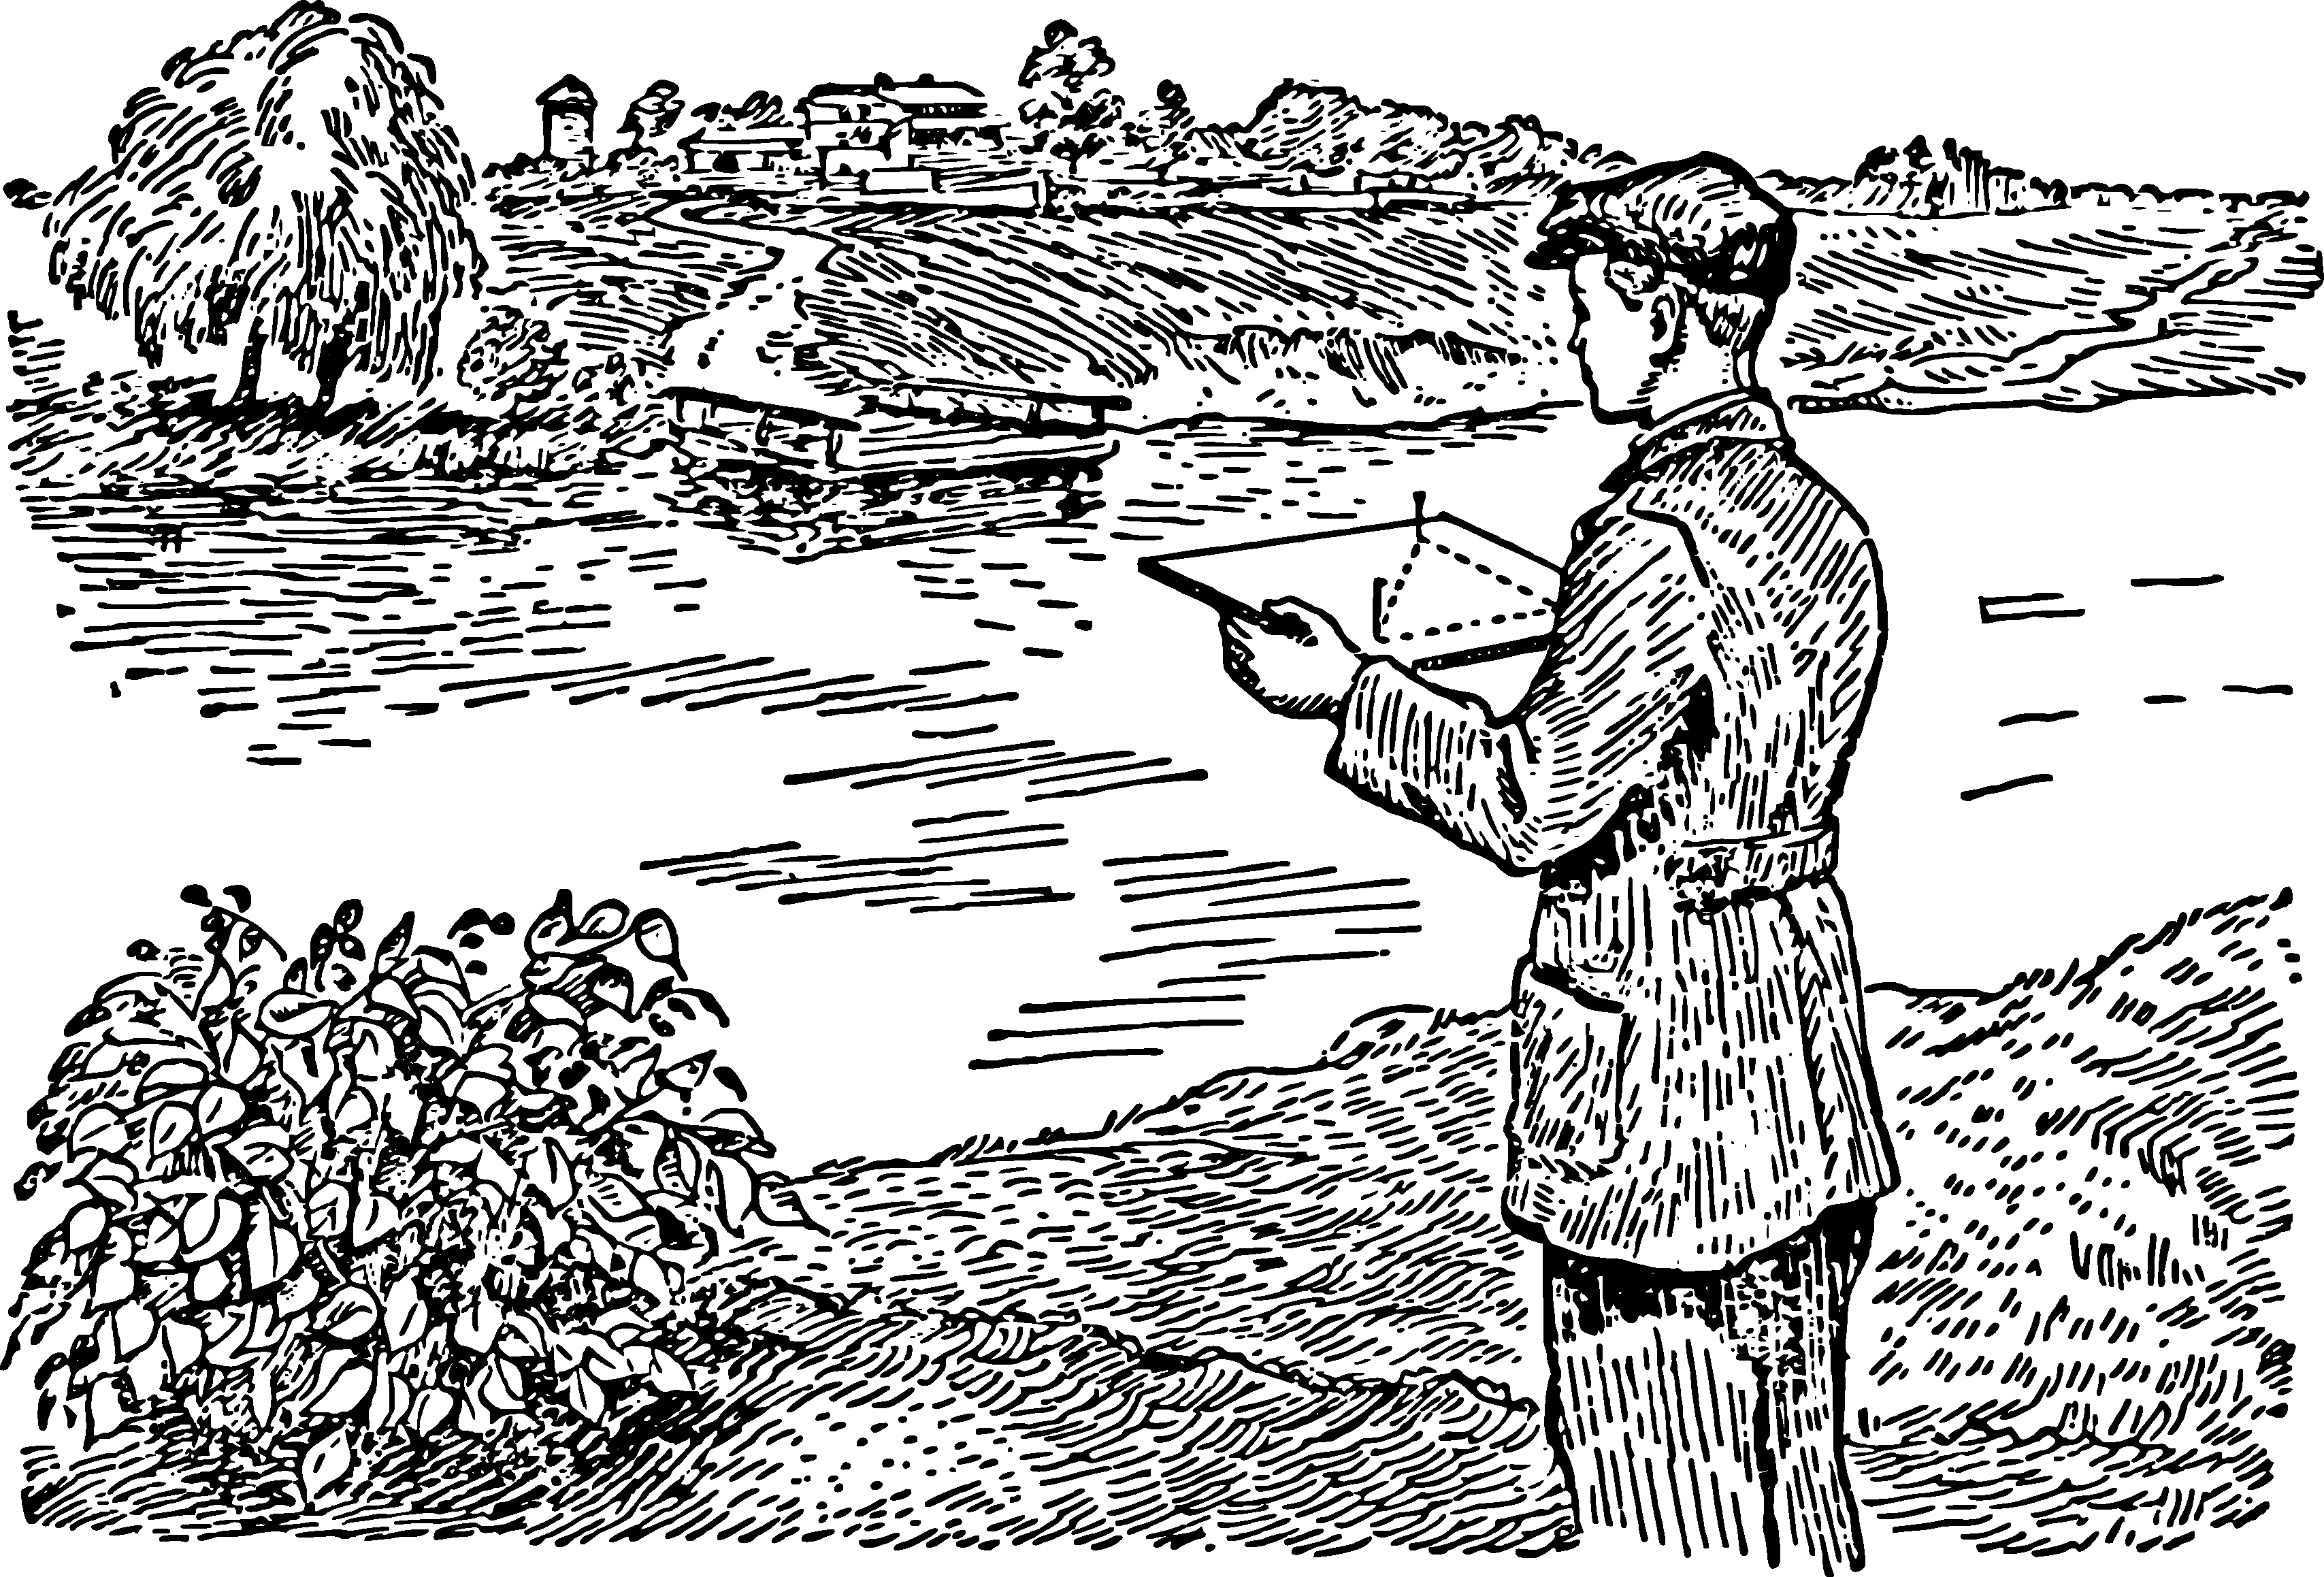
\includegraphics[width=0.9\textwidth]{figures/ch-02/fig-025.pdf}
\sidecaption{Measuring the width of the river with a pin device.\label{fig-025}}
\end{figure}

\begin{enumerate}
\item The first method requires the familiar ``device'' with three pins at the vertices of an isosceles right triangle (\figr{fig-025}). 
Let's say we need to determine the width of river $AB$ (\figr{fig-026}), standing on the bank where point $B$ is, without crossing to the opposite bank. Standing somewhere at point $C$, hold the pin device close to your eye so that, looking with one eye along the two pins, you see both covering points $B$ and $A$. It's clear that when you manage this, you will be exactly on the extension of line $AB$. 

\begin{marginfigure}[-1.5cm]%[h!]
\centering
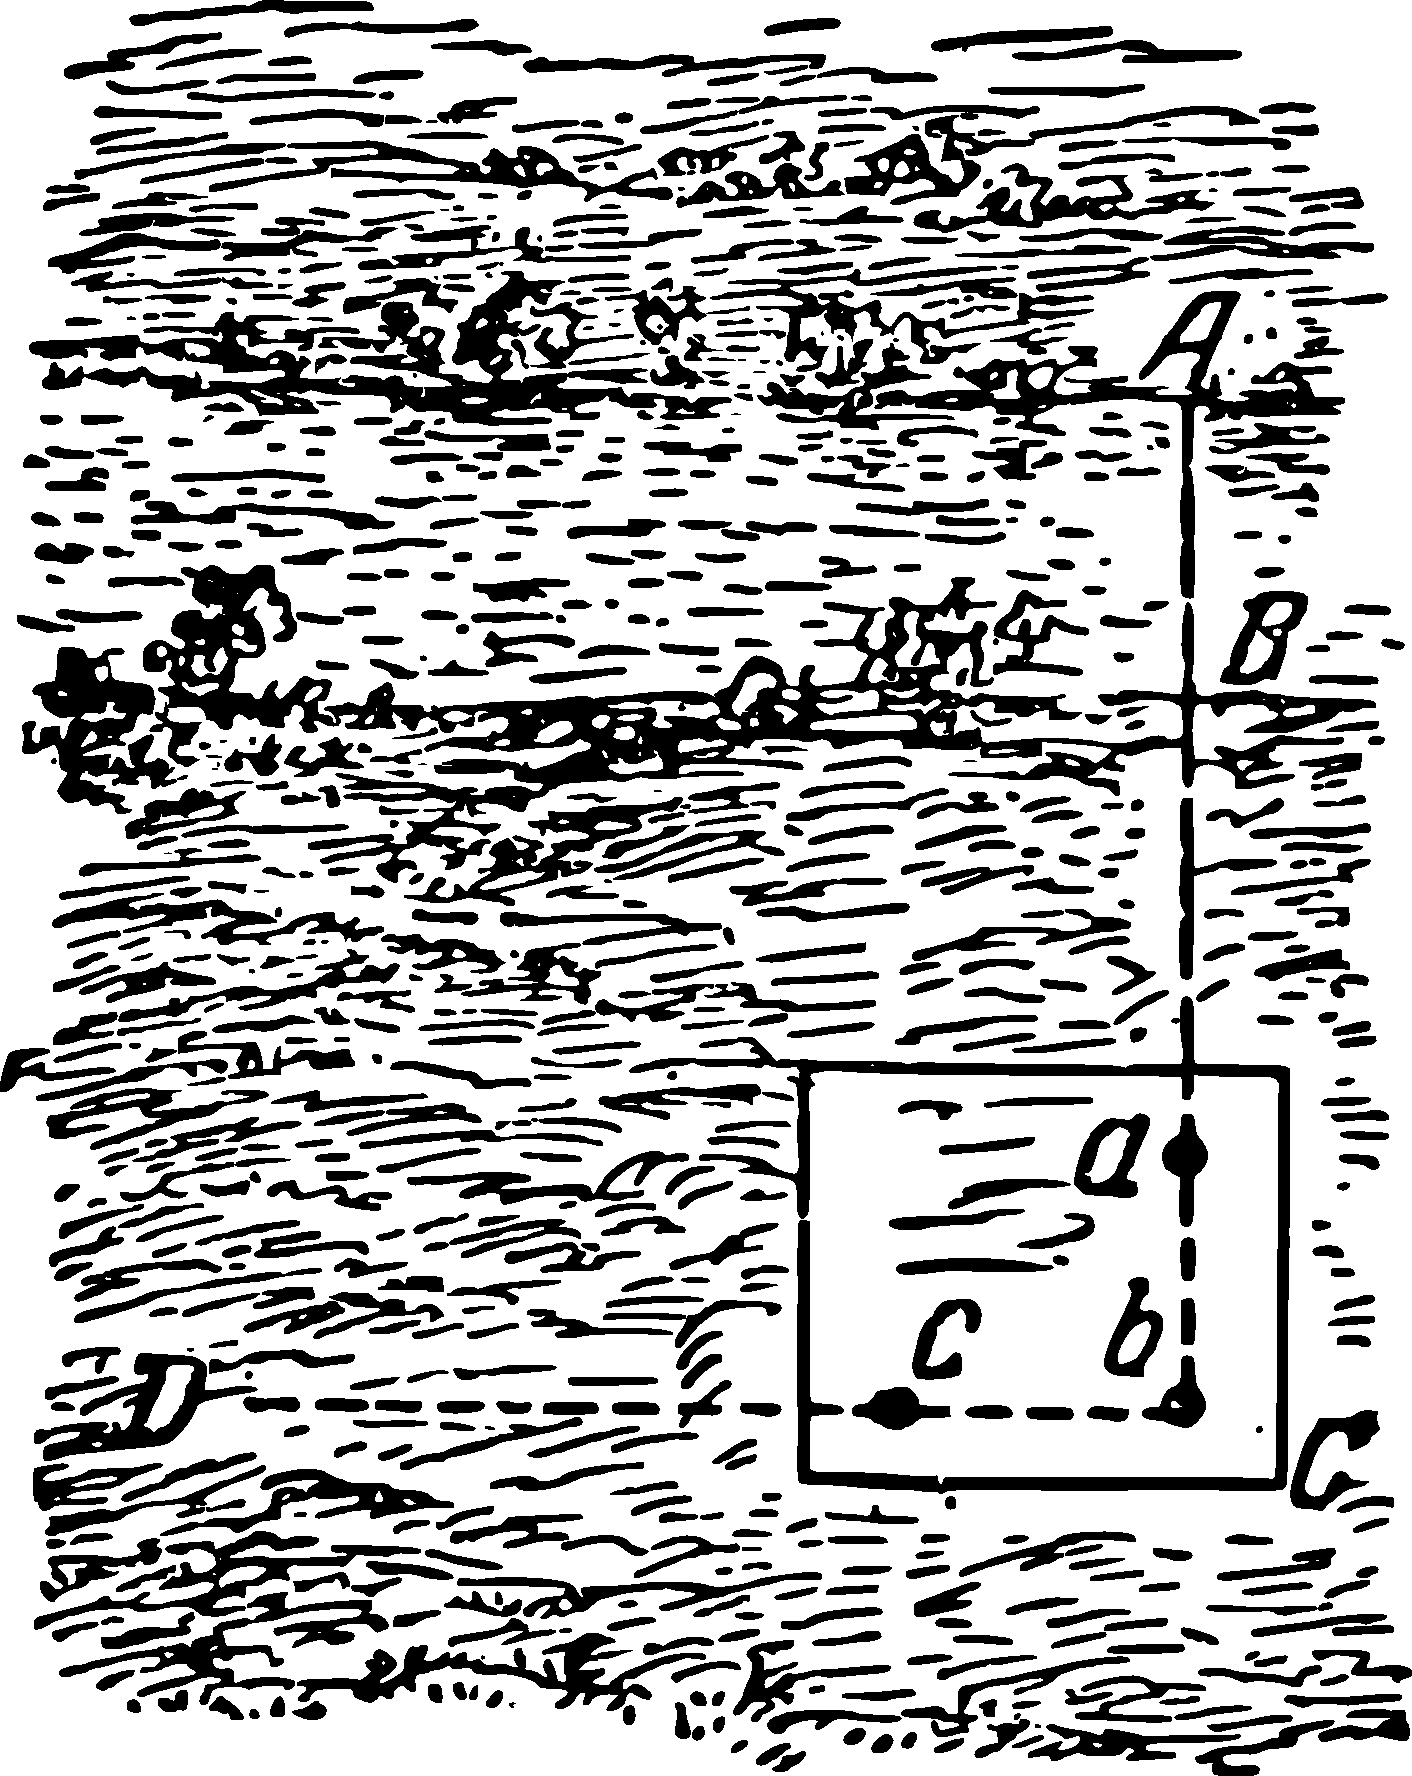
\includegraphics[width=\textwidth]{figures/ch-02/fig-026.pdf}
\sidecaption{First position of the pin device.\label{fig-026}}
\end{marginfigure}
\begin{marginfigure}[5cm]%[h!]
\centering
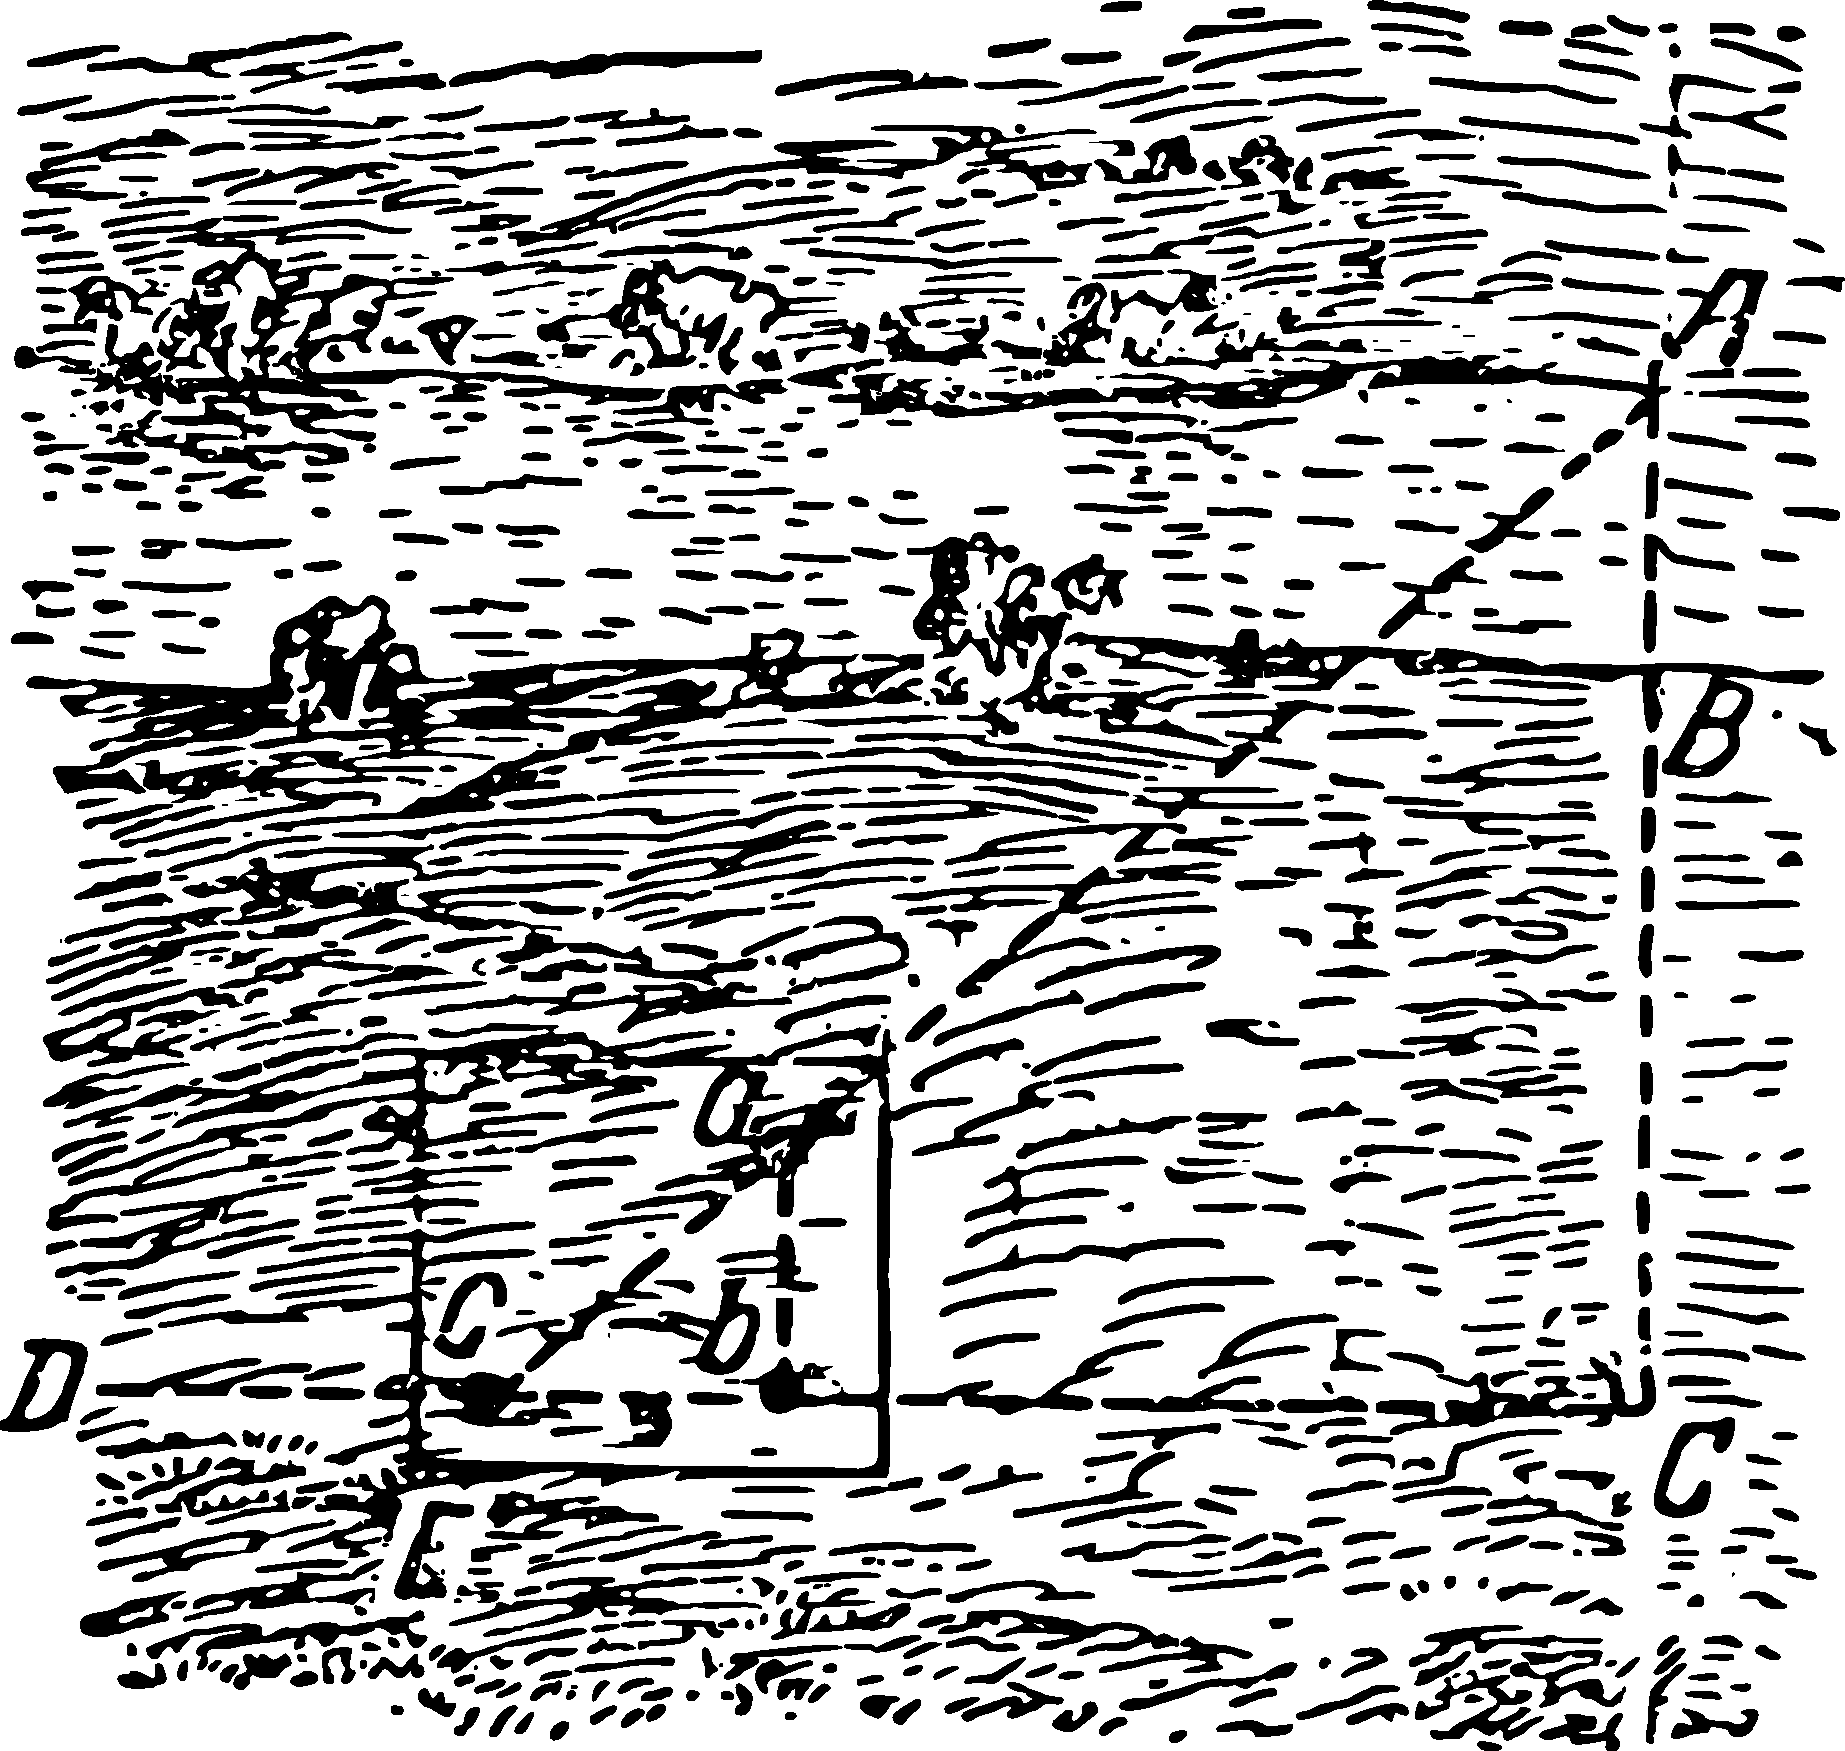
\includegraphics[width=\textwidth]{figures/ch-02/fig-027.pdf}
\sidecaption{Second position of the pin device.\label{fig-027}}
\end{marginfigure}


Now, without moving the plank of the device, look along the other two pins (perpendicular to the previous direction) and notice any point $D$ covered by these pins, i.e., lying on the line perpendicular to $AC$. After this, insert a pin at point $C$, leave this place, and go with your instrument along line $CD$ until you find a point $E$ (\figr{fig-027}), where you can simultaneously cover point $C$ for one eye with pin $b$ and point $A$ with pin $a$. This means you have found the third vertex of triangle $ACE$ on the shore, where angle $C$ is a right angle, and angle $E$ is opposite to the acute angle of the pin device, i.e., half the right angle (\ang{45}). Obviously, angle $A$ is also half right angle, i.e., $AC = CE$. If you measure the distance $CE$ even by steps, you will know the distance $AC$, and by subtracting $BC$, which is easy to measure, you will determine the desired width of the river.

It is quite inconvenient and difficult to hold the pin device still in hand; therefore, it is better to attach this plank to a stick with a pointed end and insert it vertically into the ground.

\item The second method is similar to the first. Here also, find point $C$ on the extension of $AB$ and mark line $CD$ perpendicular to $CA$ using the pin device. But then proceed differently (\figr{fig-028}). Equal distances $CE$ and $EF$ of arbitrary length are measured on the straight line $CD$, and pegs are inserted at points $E$ and $F$. Then, standing at point $F$ with a pin device, the direction $FG$ is marked out perpendicular to $FC$. Now, walking along $FG$, find a point $H$ on this line from which point $A$ seems to be covered by point $E$. This will mean that points $H$, $E$, and $A$ lie on the same straight line.

\begin{figure}[h!]
\centering
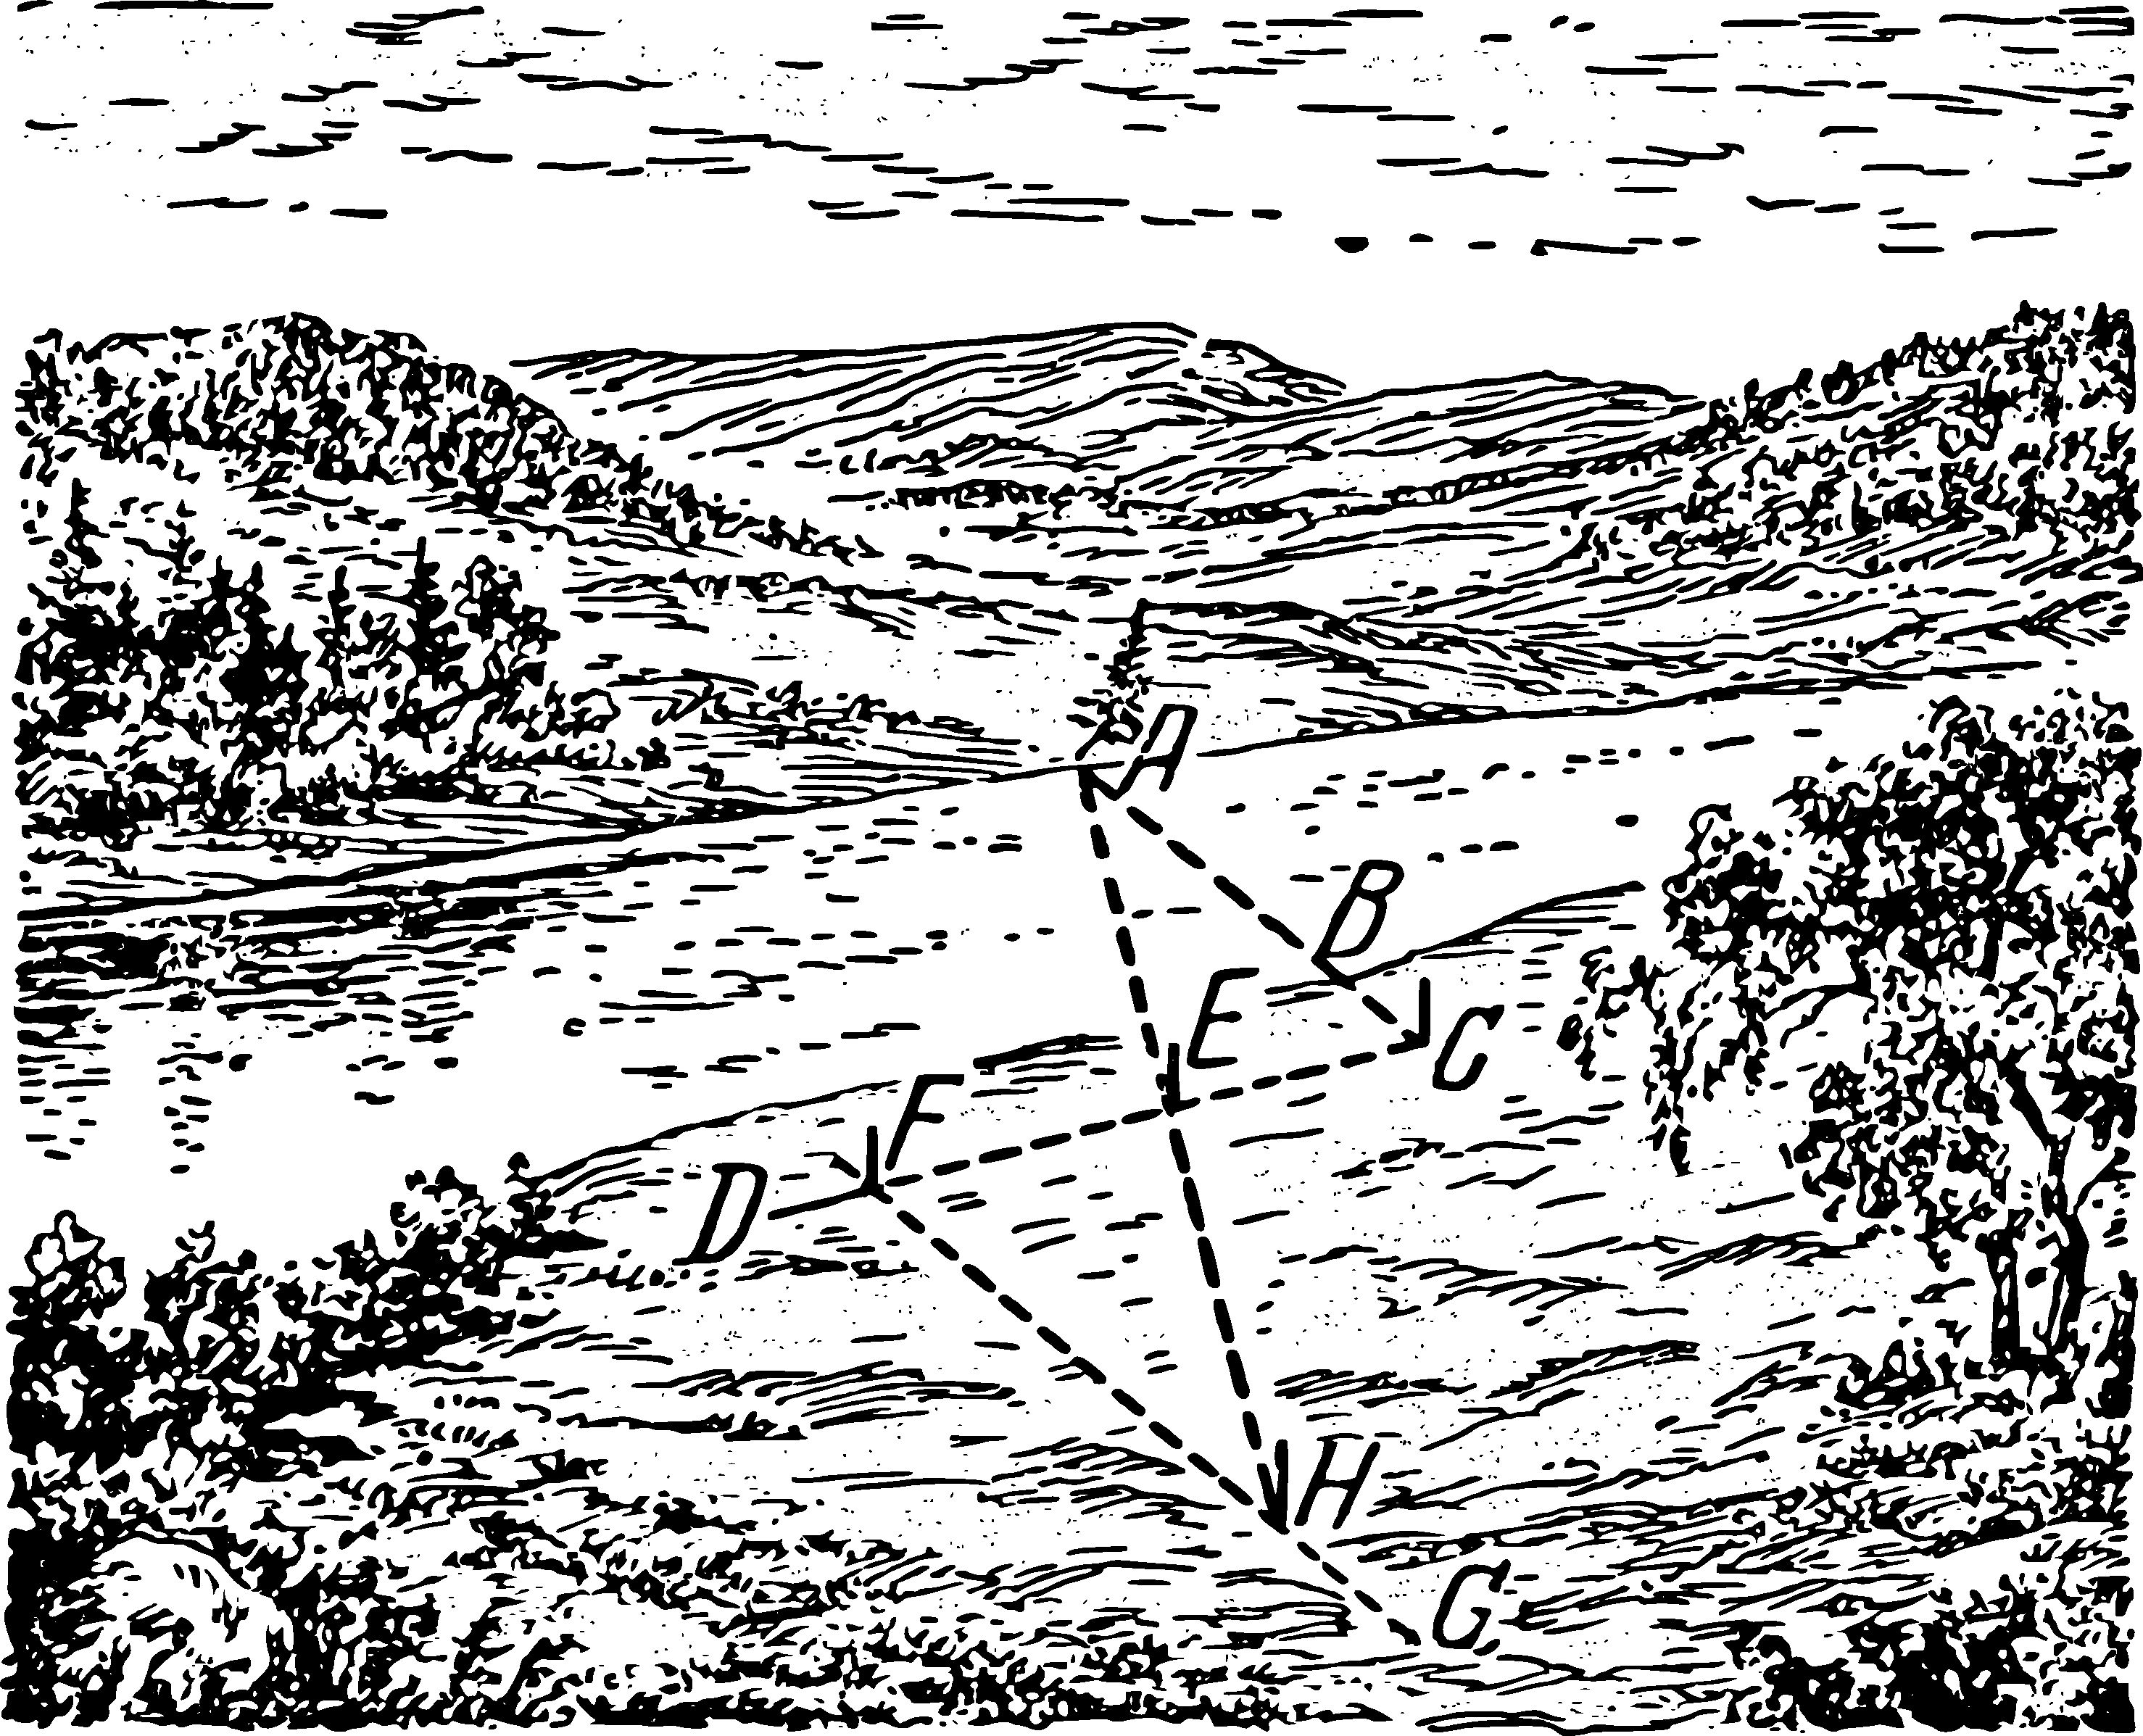
\includegraphics[width=0.9\textwidth]{figures/ch-02/fig-028.pdf}
\sidecaption{ Using the congruence criteria of triangles to find the width of the river.\label{fig-028}}
\end{figure}

The problem is solved: the distance $FH$ is equal to the distance $AC$, from which it is only necessary to subtract $BC$ to find the desired width of the river (the reader, of course, will guess for himself why $FH$ is equal to $AC$).

This method requires more space than the first one; if the terrain allows executing both methods, it is useful to verify one result by another.
\begin{figure}[h!]
\centering
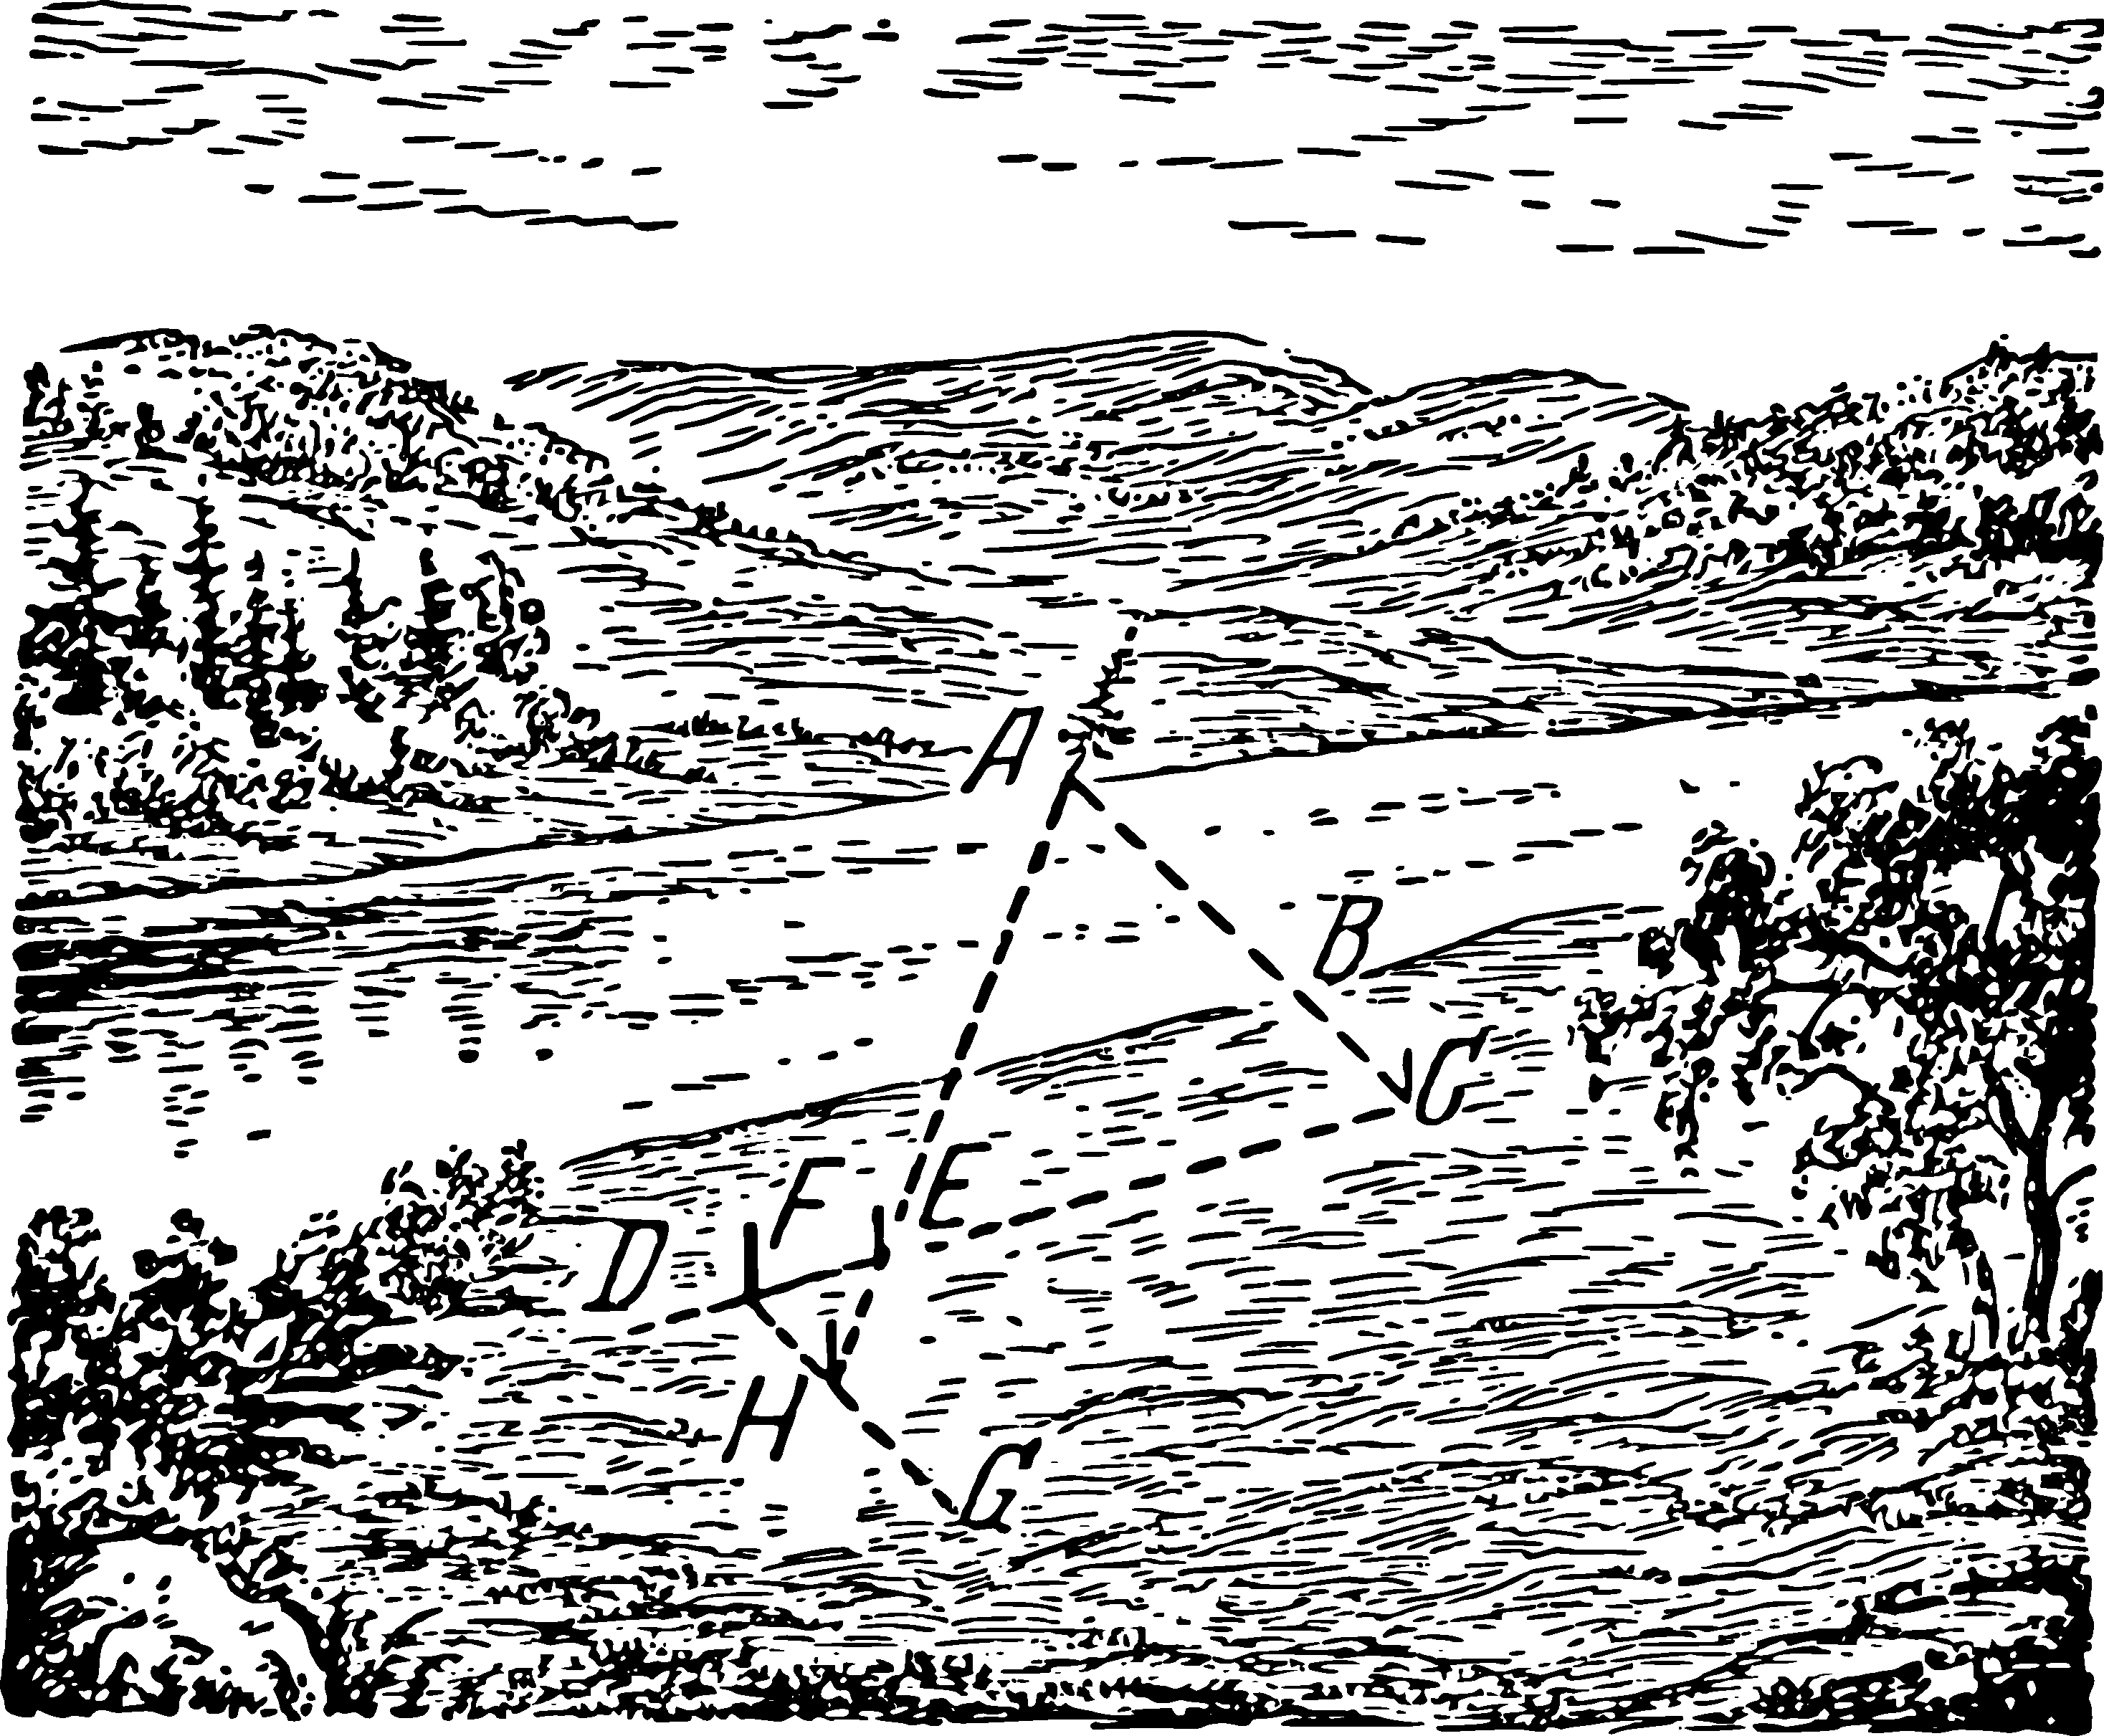
\includegraphics[width=0.9\textwidth]{figures/ch-02/fig-029.pdf}
\sidecaption{Using the similarity criteria of triangles to find the width of the river.\label{fig-029}}
\end{figure}

\item The method described above can be modified: instead of measuring equal distances on the straight line $CF$, measure one distance several times smaller than the other. For example (\figr{fig-029}), $FE$ is measured four times less than $EC$, and then we proceed as before: in the direction $FG$, perpendicular to $FC$, we find a point $H$ from which the peg $E$ appears to cover point $A$. But now $FH$ is no longer equal to $AC$, but four times smaller than this distance: triangles $ACE$ and $EFH$ are not congruent here, but similar (they have equal angles with unequal sides). From the similarity of triangles follows the proportion:
\begin{equation*}%
\frac{AC}{FH} = \frac{CE}{EF} = \frac{4}{1}
\end{equation*}
Therefore, by measuring $FH$ and multiplying the result by 4, we get the distance $AC$, and by subtracting $BC$, we find the desired width of the river.

This method, as we can see, requires less space and is therefore more convenient to perform than the previous one.




\item The fourth method is based on the property of a right triangle that if one of its acute angles is \ang{30}, then the length of the cathetus is half the hypotenuse. It is very easy to verify the correctness of this. 

Let angle $B$ of right triangle $ABC$ (\figr{fig-030}, left) be \ang{30}; we will prove that in this case, $AC = \nicefrac{1}{2}\, AB$. Rotate triangle $ABC$ around $BC$ so that it is symmetric with its initial position (\figr{fig-030}, right), forming figure $ABD$; line $AC$ is straight because both angles at point $C$ are right angles. In triangle $ABD$, angle $\angle A = \ang{60}$, angle $ABD$, composed of two \ang{30} angles, is also equal to \ang{60}. Therefore, $AD = BD$ as sides opposite equal angles. But $AC = \nicefrac{1}{2} \,AD$, therefore,
\begin{marginfigure}%[5cm]%[h!]
\centering
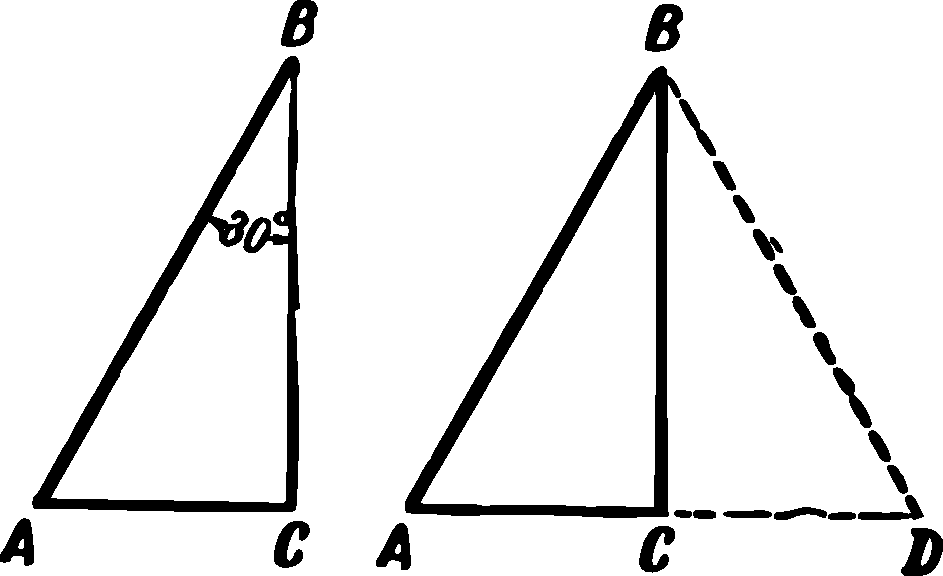
\includegraphics[width=\textwidth]{figures/ch-02/fig-030.pdf}
\sidecaption{When the cathetus is half the hypotenuse.\label{fig-030}}
\end{marginfigure}
\begin{equation*}%
AC = \frac{1}{2} AB.
\end{equation*}
Wishing to take advantage of this property of the triangle, we must arrange the pins on the board so that their bases represent a right triangle in which the cathetus is half the hypotenuse. With this device, we place ourselves at point $C$ (\figr{fig-031}) so that the direction $AC$ coincides with the hypotenuse of the pin triangle. 
\begin{marginfigure}%[5cm]%[h!]
\centering
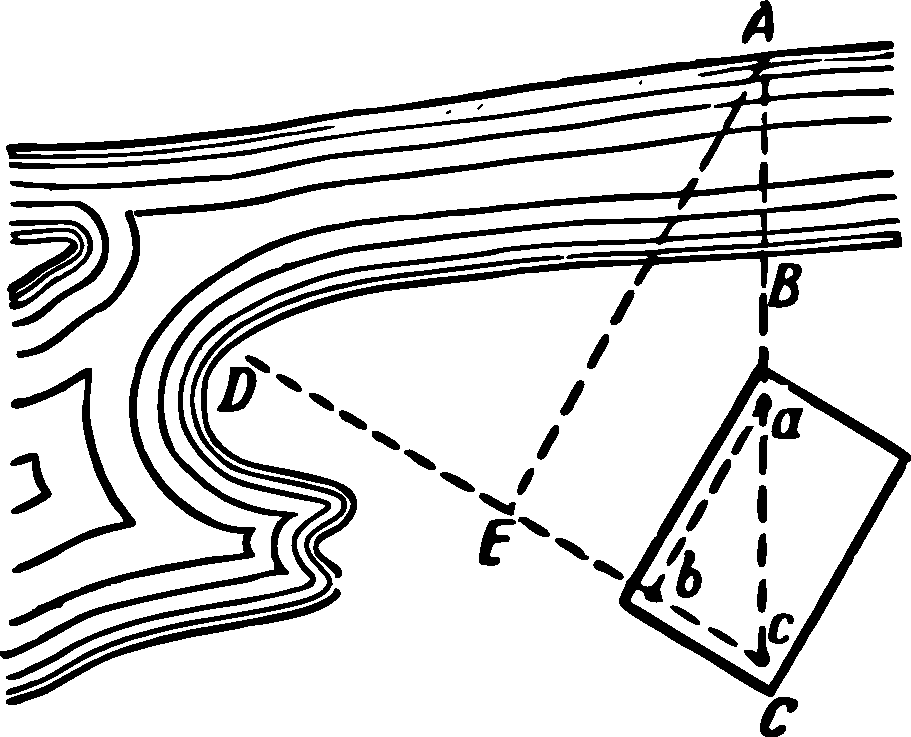
\includegraphics[width=\textwidth]{figures/ch-02/fig-031.pdf}
\sidecaption{The scheme of application of a right-angled triangle with a 30° angle.\label{fig-031}}
\end{marginfigure}
Looking along the short cathetus of this triangle, mark the direction $CD$ and find a point $E$ on it so that the direction $EA$ is perpendicular to $CD$ (this is done using the same pin device). It is easy to see that the distance $CE$ -- the cathetus lying opposite the angle of \ang{30} -- is equal to half of $AC$. Therefore, by measuring $CE$, doubling this distance and subtracting $BC$, we obtain the desired width of the $AB$ river.

\end{enumerate}

Here are four easily executable methods, with which it is always possible, without crossing to the other bank, to measure the width of the river with quite satisfactory accuracy. We will not consider methods that require the use of more complex instruments (even homemade ones) here.

\section{Using a visor}
\label{sec-2.2}

Here's how this method came in handy for Senior Sergeant Kupriyanov in frosty conditions.\sidenote{See the footnote on page~\pageref{ref-21}.} His detachment was ordered to measure the width of the river, across which they were to organise a crossing\ldots{}

Approaching a bush near the river, Kupriyanov's detachment took cover, and Kupriyanov himself, along with soldier Karpov, moved closer to the riverbank, from where the fascist-occupied shore was clearly visible. In such conditions, measuring the width of the river had to be done by eye.

``Come on, Karpov, how much?'' Kupriyanov asked.

``I think no more than 100-110 meters,'' Karpov replied. Kupriyanov agreed with his scout, but for control, he decided to measure the width of the river using a ``visor.''

\begin{figure}[h!]
\centering
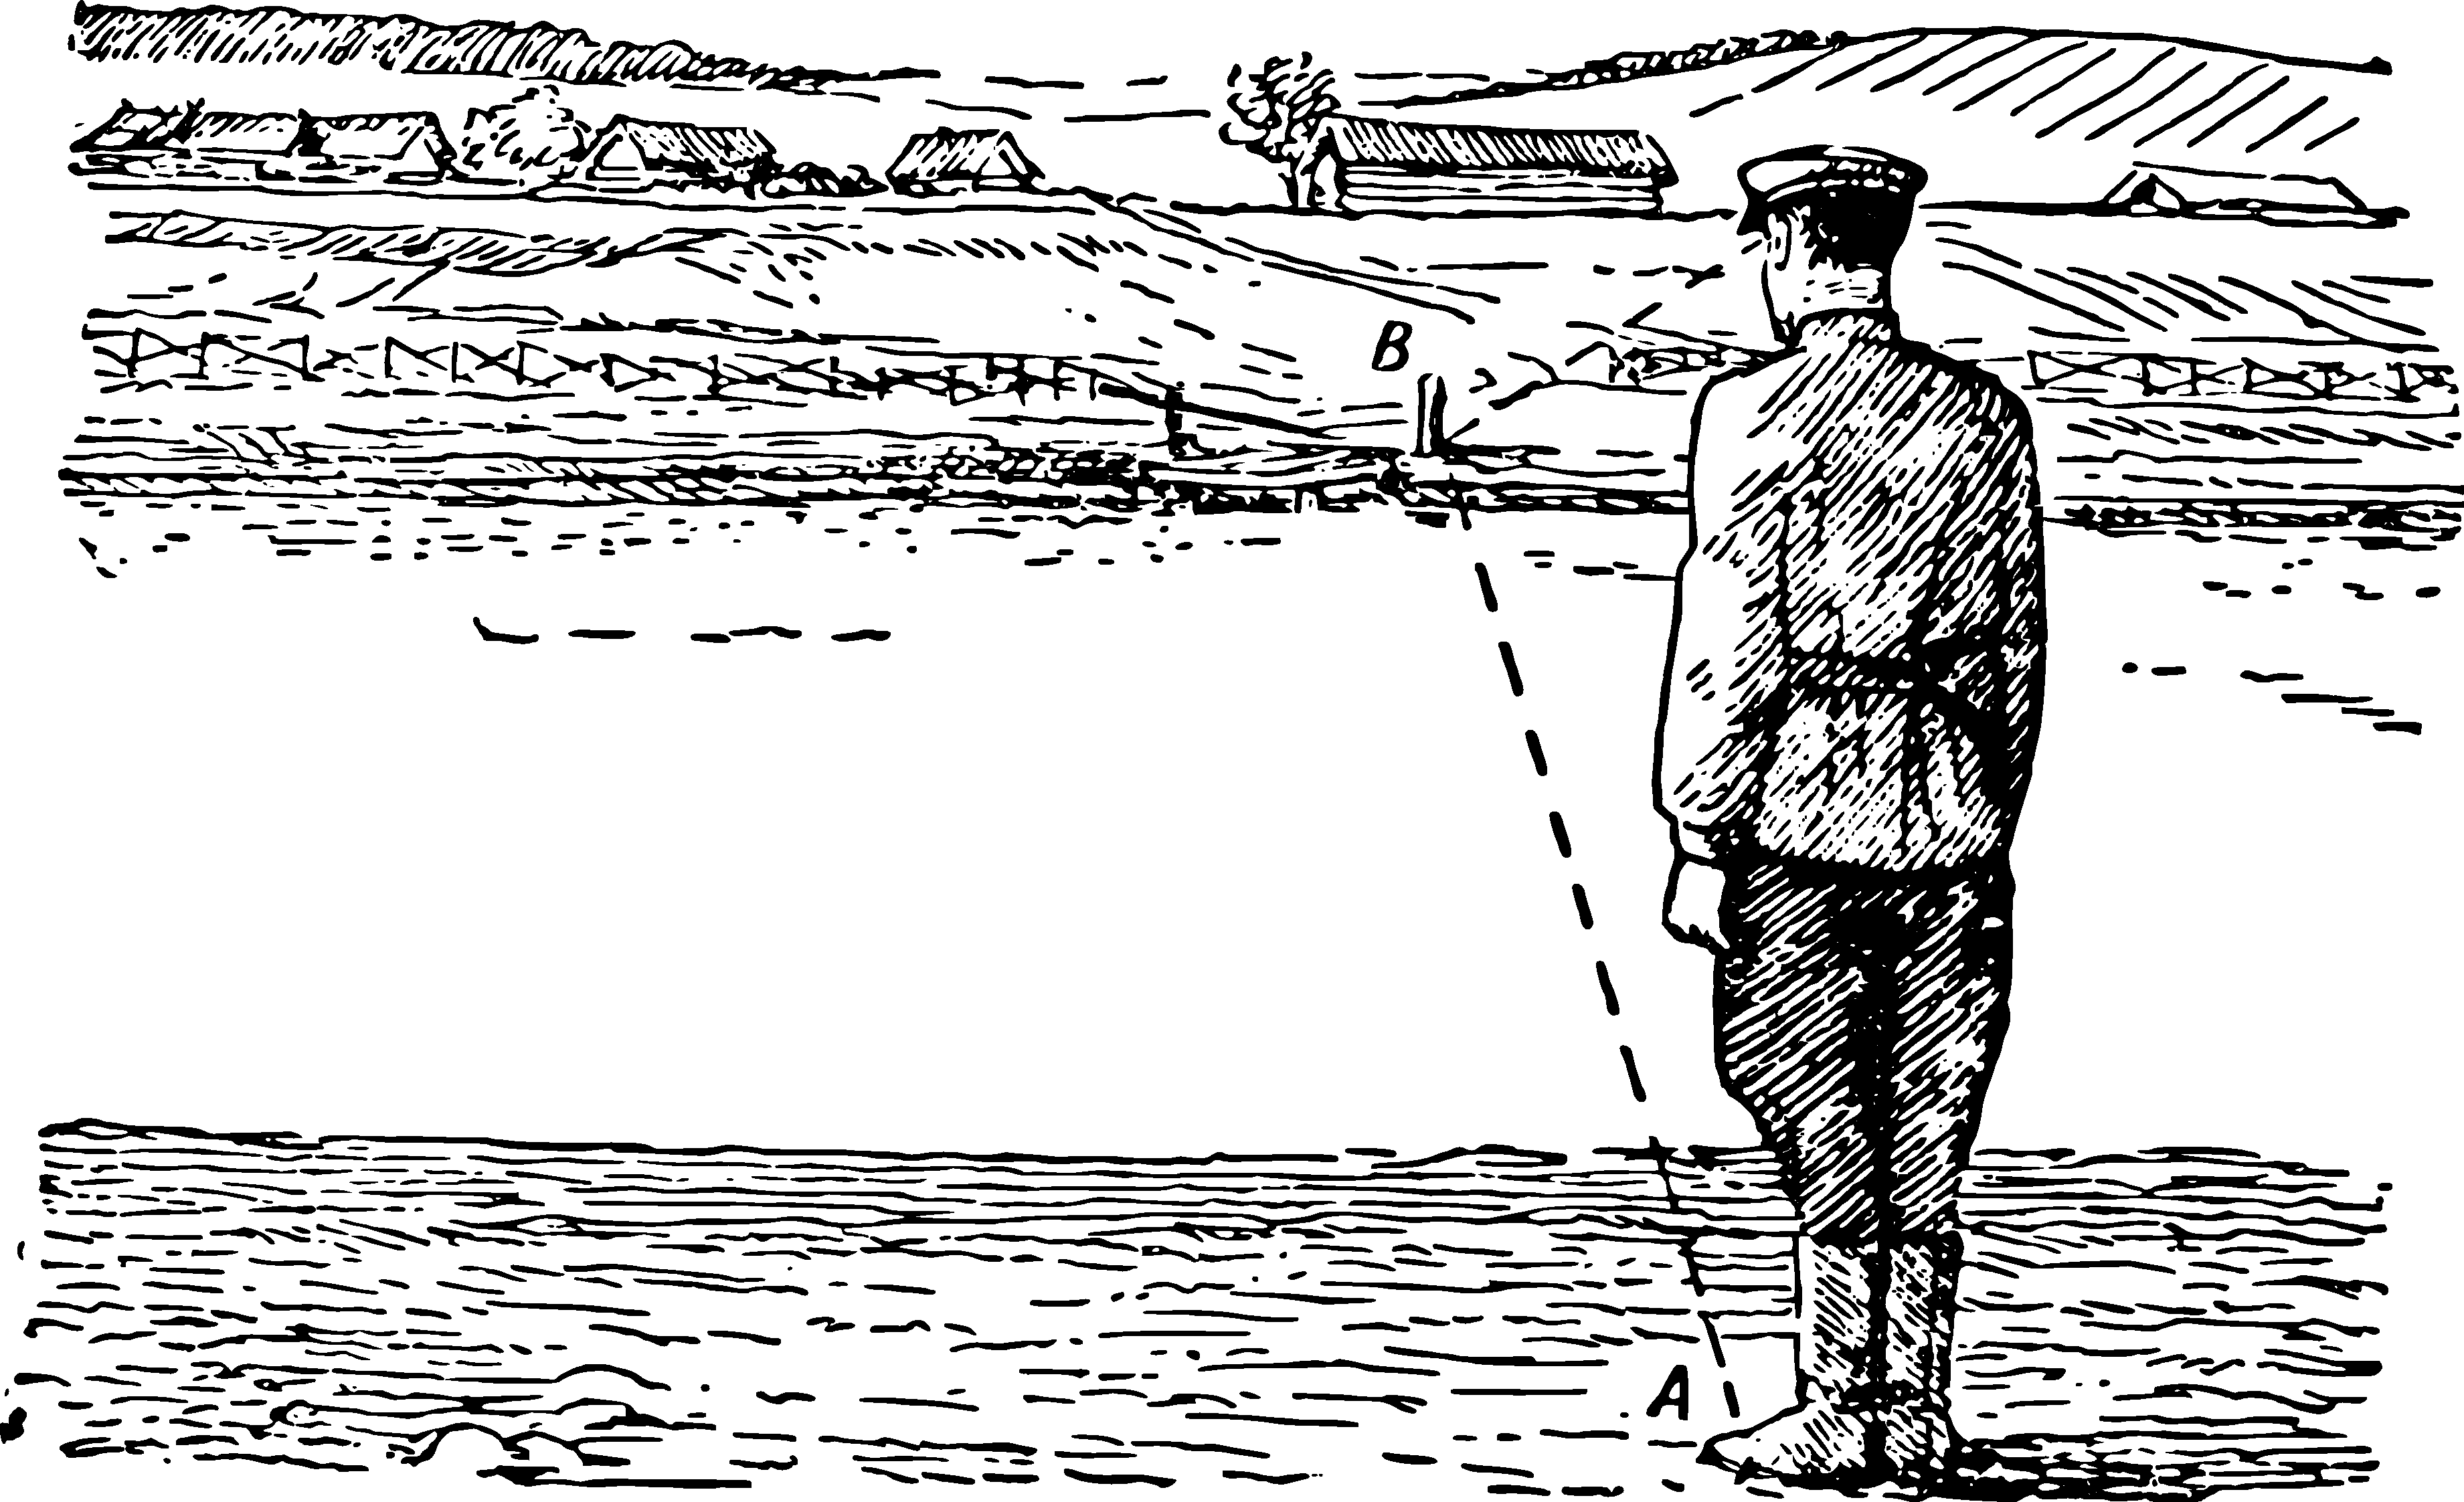
\includegraphics[width=0.9\textwidth]{figures/ch-02/fig-032.pdf}
\sidecaption{Observing a point on the opposite bank from under the visor.\label{fig-032}}
\end{figure}

This method is simple. You have to face the river and pull the visor over your eyes so that the lower edge of the visor precisely aligns with the line of the opposite bank (see \figr{fig-032}). The visor can be replaced with the palm of your hand or a notepad, tightly pressed edge to your forehead. Then, without changing the position of your head, you need to turn to the right or left, or even backward (towards the side where the area available for measuring the distance is more level) and notice the farthest point visible from under the visor (palm, notepad).

The distance to this point will be approximately equal to the width of the river.

Kupriyanov utilized this method. He quickly stood up in the bushes, pressed a notepad to his forehead, then quickly turned and aimed at the distant point. Then, together with Karpov, he crawled to that point, measuring the distance with a rope. It turned out to be 105 meters.

Kupriyanov reported the data he obtained to the command.

\ques Provide a geometric explanation for the ``visor'' method.

\begin{figure}[h!]
\centering
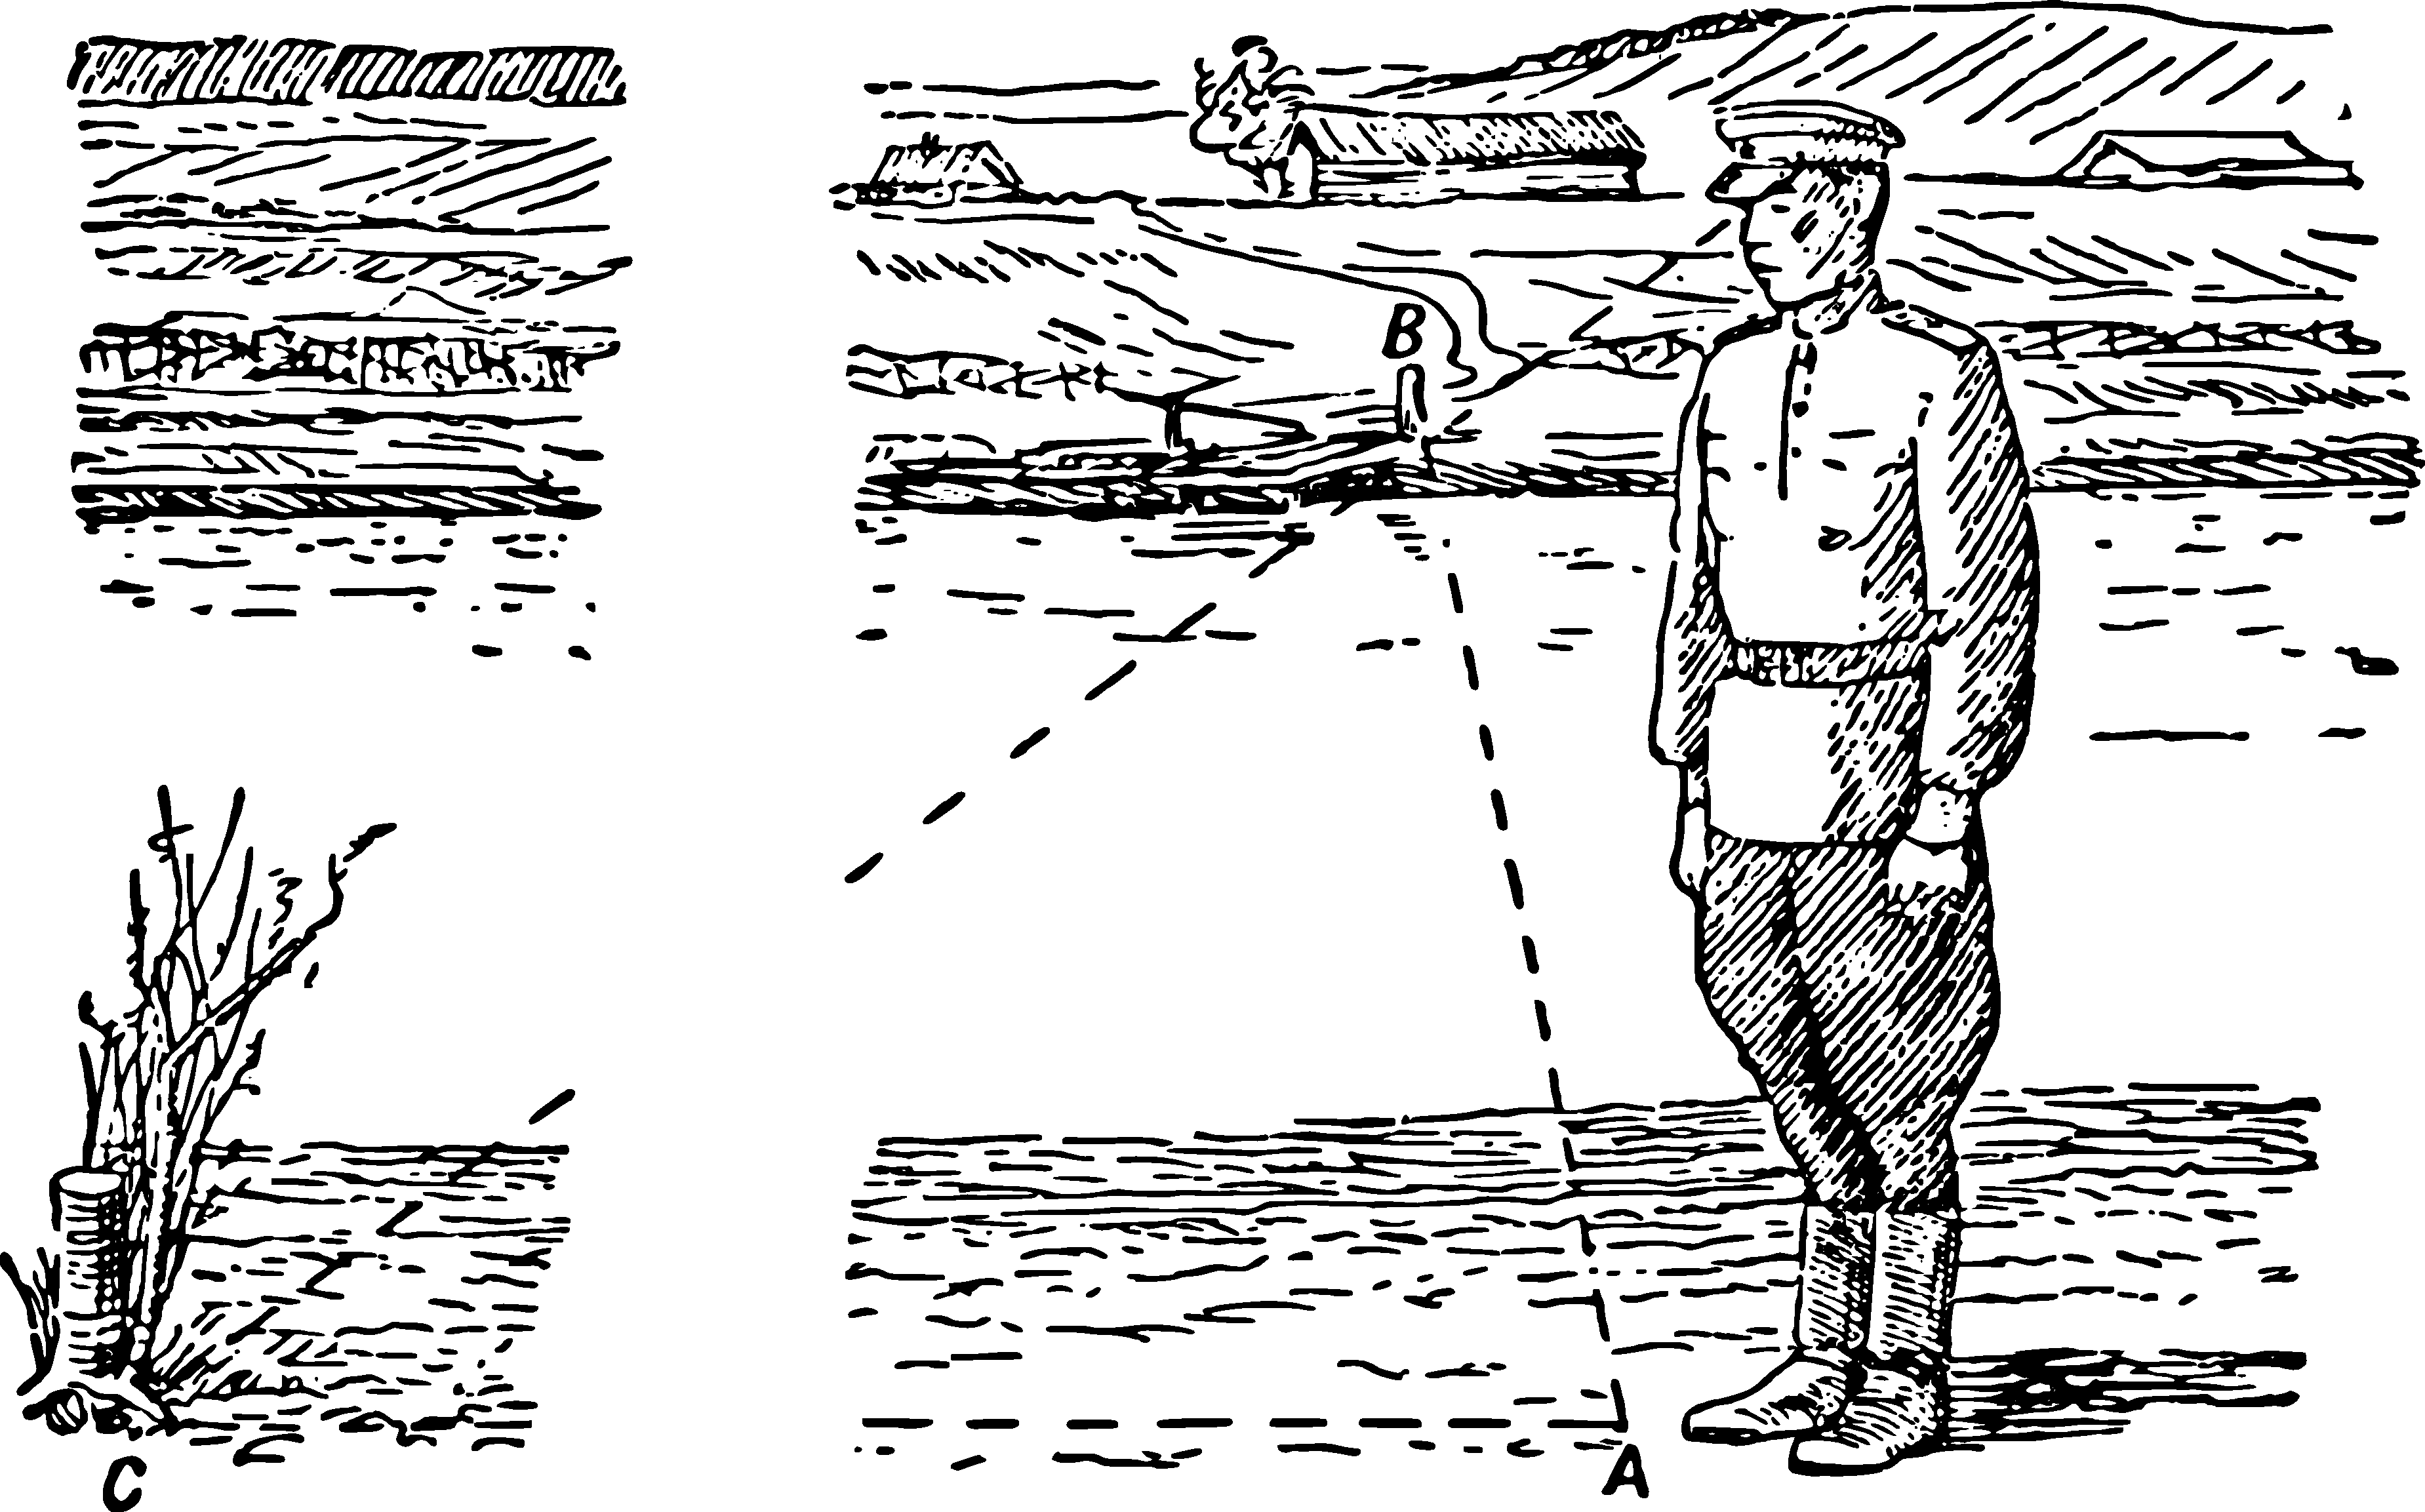
\includegraphics[width=0.9\textwidth]{figures/ch-02/fig-033.pdf}
\sidecaption{In the same way, you can aim at a point on your own bank.\label{fig-033}}
\end{figure}

\ans The line of sight, touching the edge of the visor (palm, notepad), is initially directed towards the line of the opposite bank (see \figr{fig-032}). When a person turns, the line of sight, like the leg of a compass, describes a circle, and then $AC = AB$ as the radii of the same circle (see \figr{fig-033}). 

\section{The Length Of An Island}

\ques Now we are faced with a more challenging task. Standing by the river or lake, you see an island (see \figr{fig-034}) whose length you wish to measure without leaving the shore. Is it possible to carry out such a measurement?

Although in this case, both ends of the measured line are inaccessible to us, the problem is still entirely solvable, and without complex instruments.

\begin{figure}[h!]
\centering
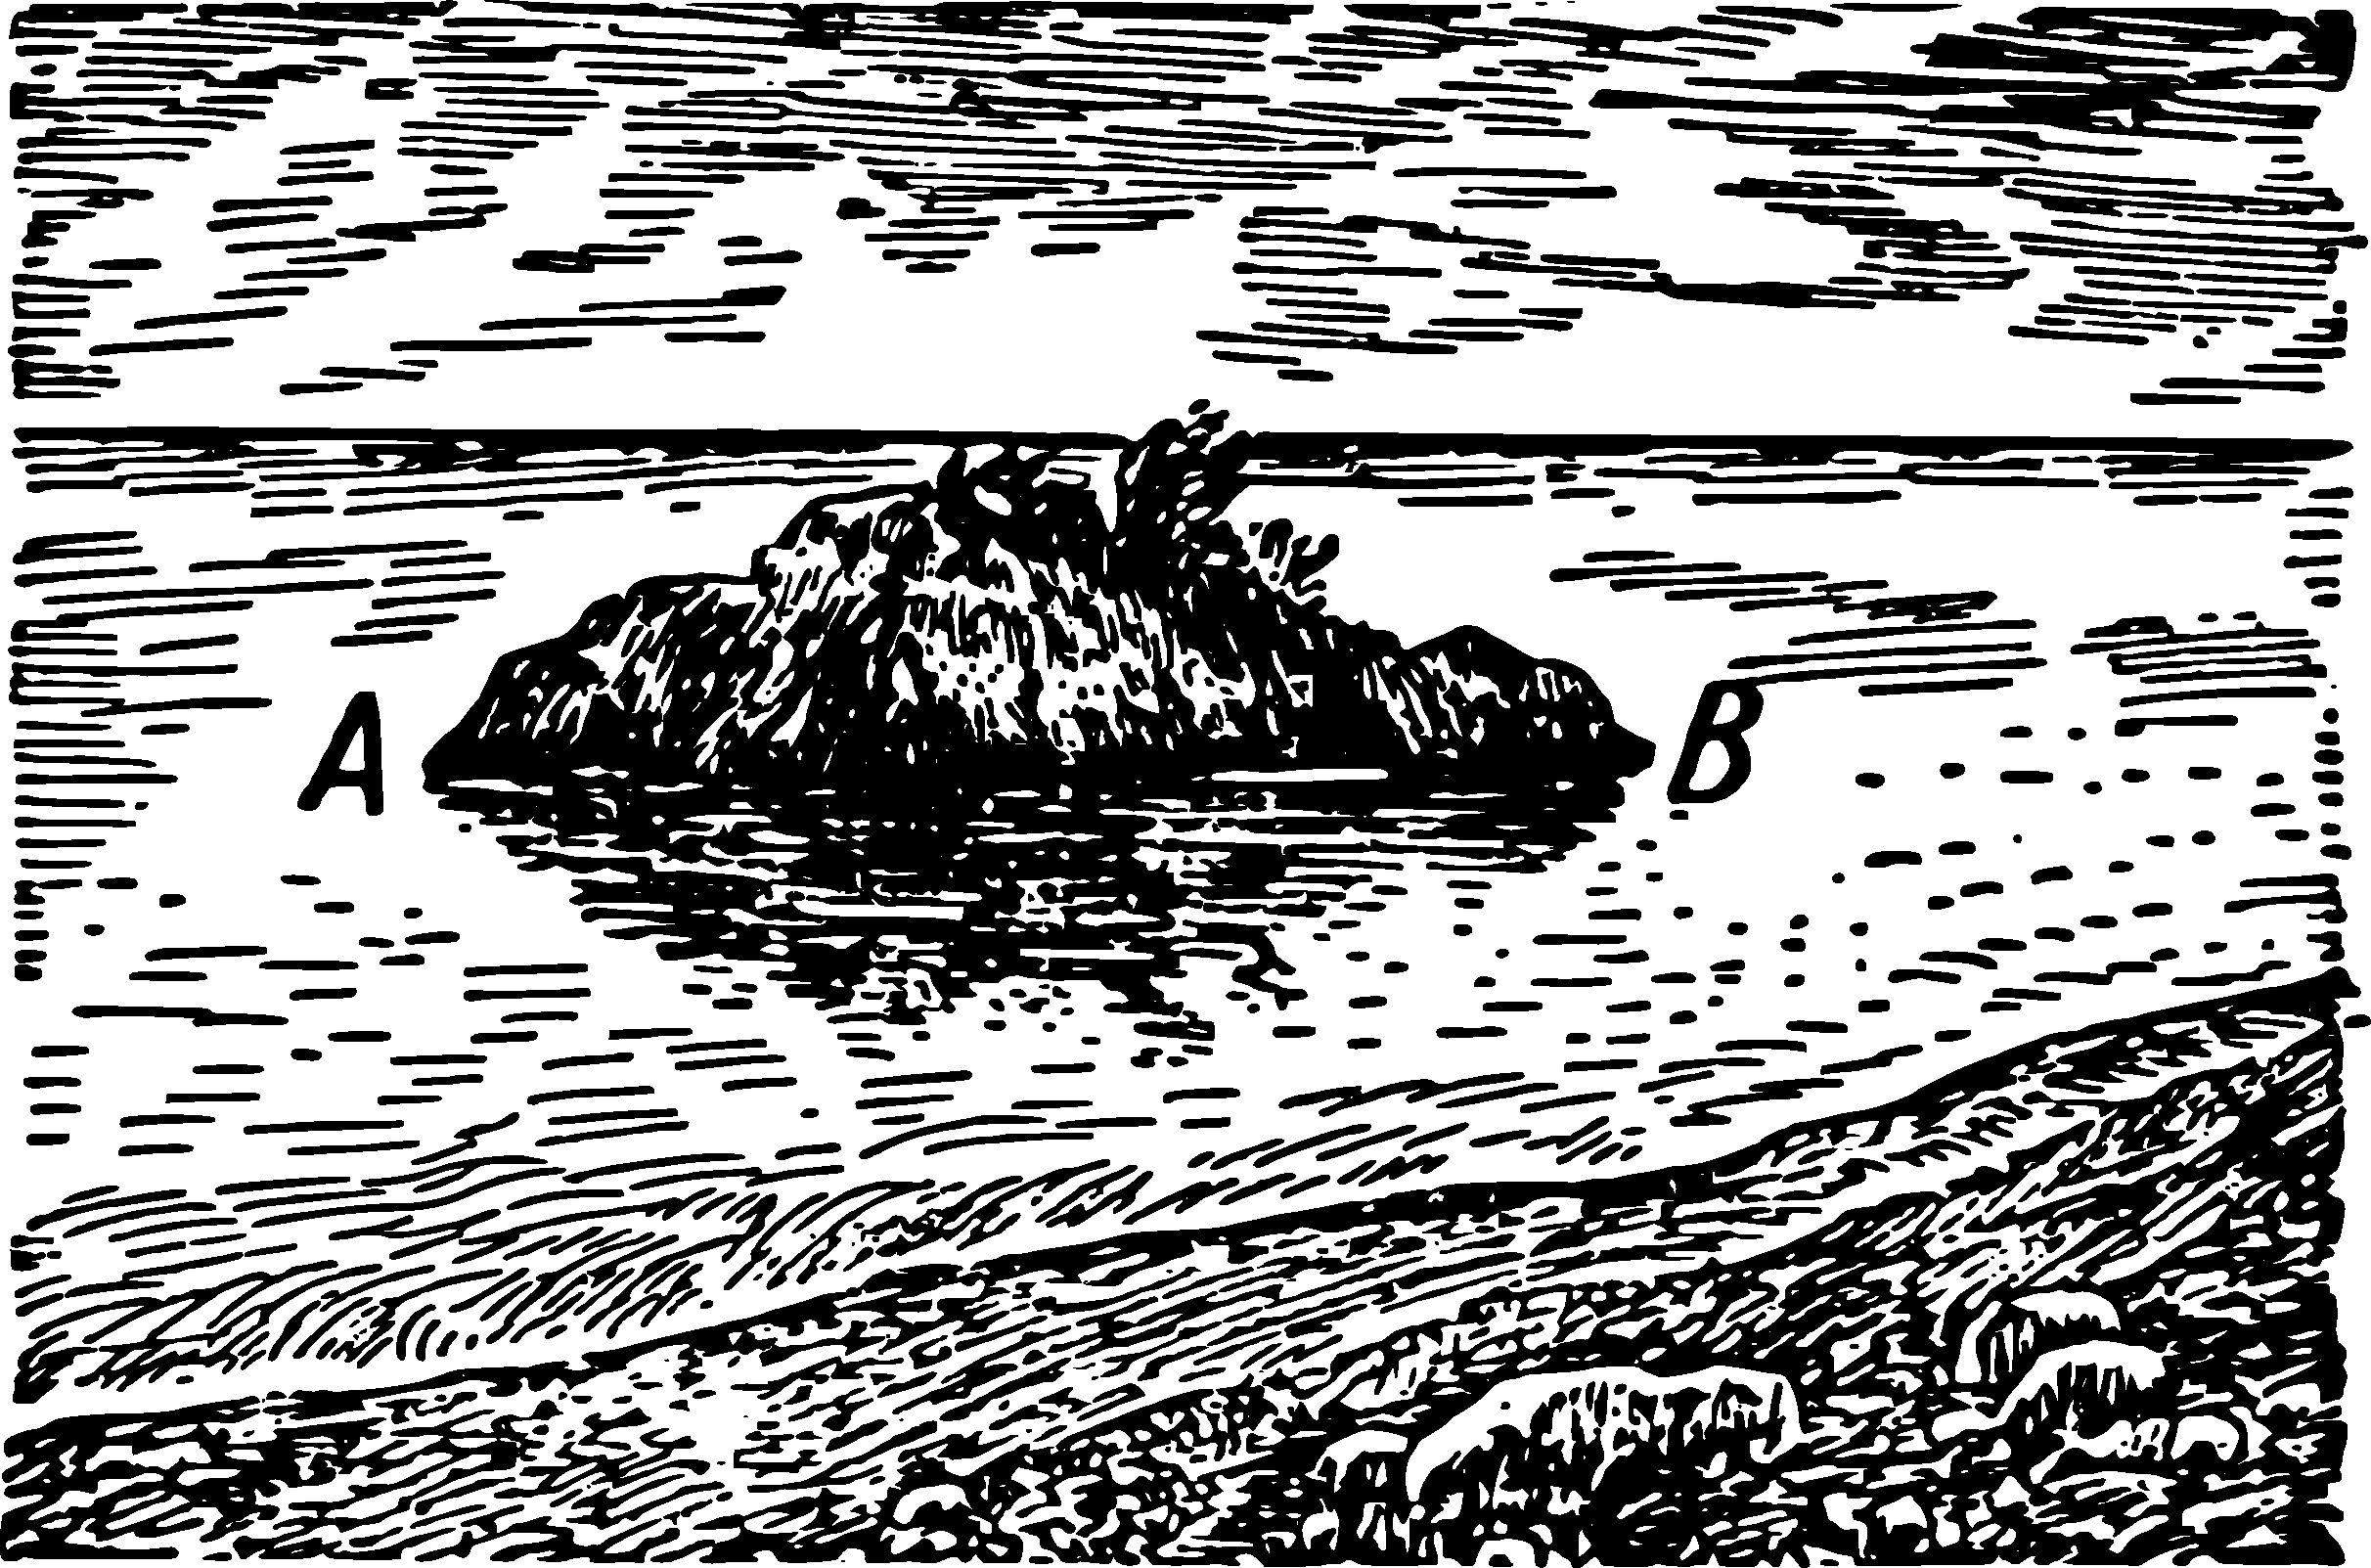
\includegraphics[width=0.9\textwidth]{figures/ch-02/fig-034.pdf}
\sidecaption{How to determine the length of the island.\label{fig-034}}
\end{figure}


\ans To measure the length of an island without leaving the shore, you can use the following method. Choose arbitrary points $P$ and $Q$ on the shore and place stakes in them. Then find points $M$ and $N$ on the line $PQ$ such that the directions $AM$ and $BM$ form right angles with the direction of $PQ$ (this can be done using a compass). In the middle of the distance $MN$, place a stake $O$ and find on the extension of the line $AM$ a point $C$ from which the stake $O$ appears to cover point $B$. Similarly, on the extension of $BN$, find point $D$ from which stake $O$ appears to cover the end $A$ of the island. The distance $CD$ will be the desired length of the island.

\begin{marginfigure}[-3cm]%[h!]
\centering
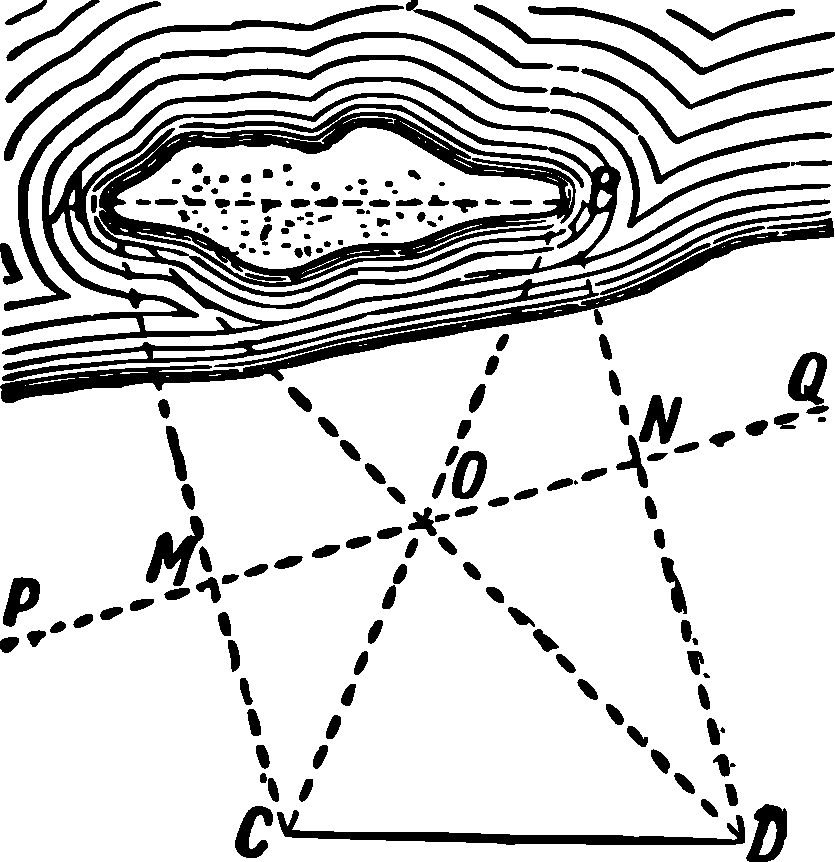
\includegraphics[width=\textwidth]{figures/ch-02/fig-035.pdf}
\sidecaption{We use the properties of congruent right triangles to find the length of an isalnd.\label{fig-035}}
\end{marginfigure}

This can be easily proved. Consider the right triangles $AMO$ and $OND$; in them, the legs $MO$ and $NO$ are equal, and the angles $AOM$ and $NOD$ are also equal, therefore, the triangles are equal, and $AO = OD$. Similarly, it can be proved that $BO = OC$. By comparing the triangles $ABO$ and $COD$, it can be seen that their distances $AB$ and $CD$ are equal.

\section{A pedestrian on the opposite bank}
\label{sec-2.3}

\ques As you walk along the riverbank, you see a person on the other side, and you can clearly distinguish their steps. Can you, without moving from your spot, determine at least approximately the distance between them and you? You have no instruments at hand.

\begin{figure}[h!]
\centering
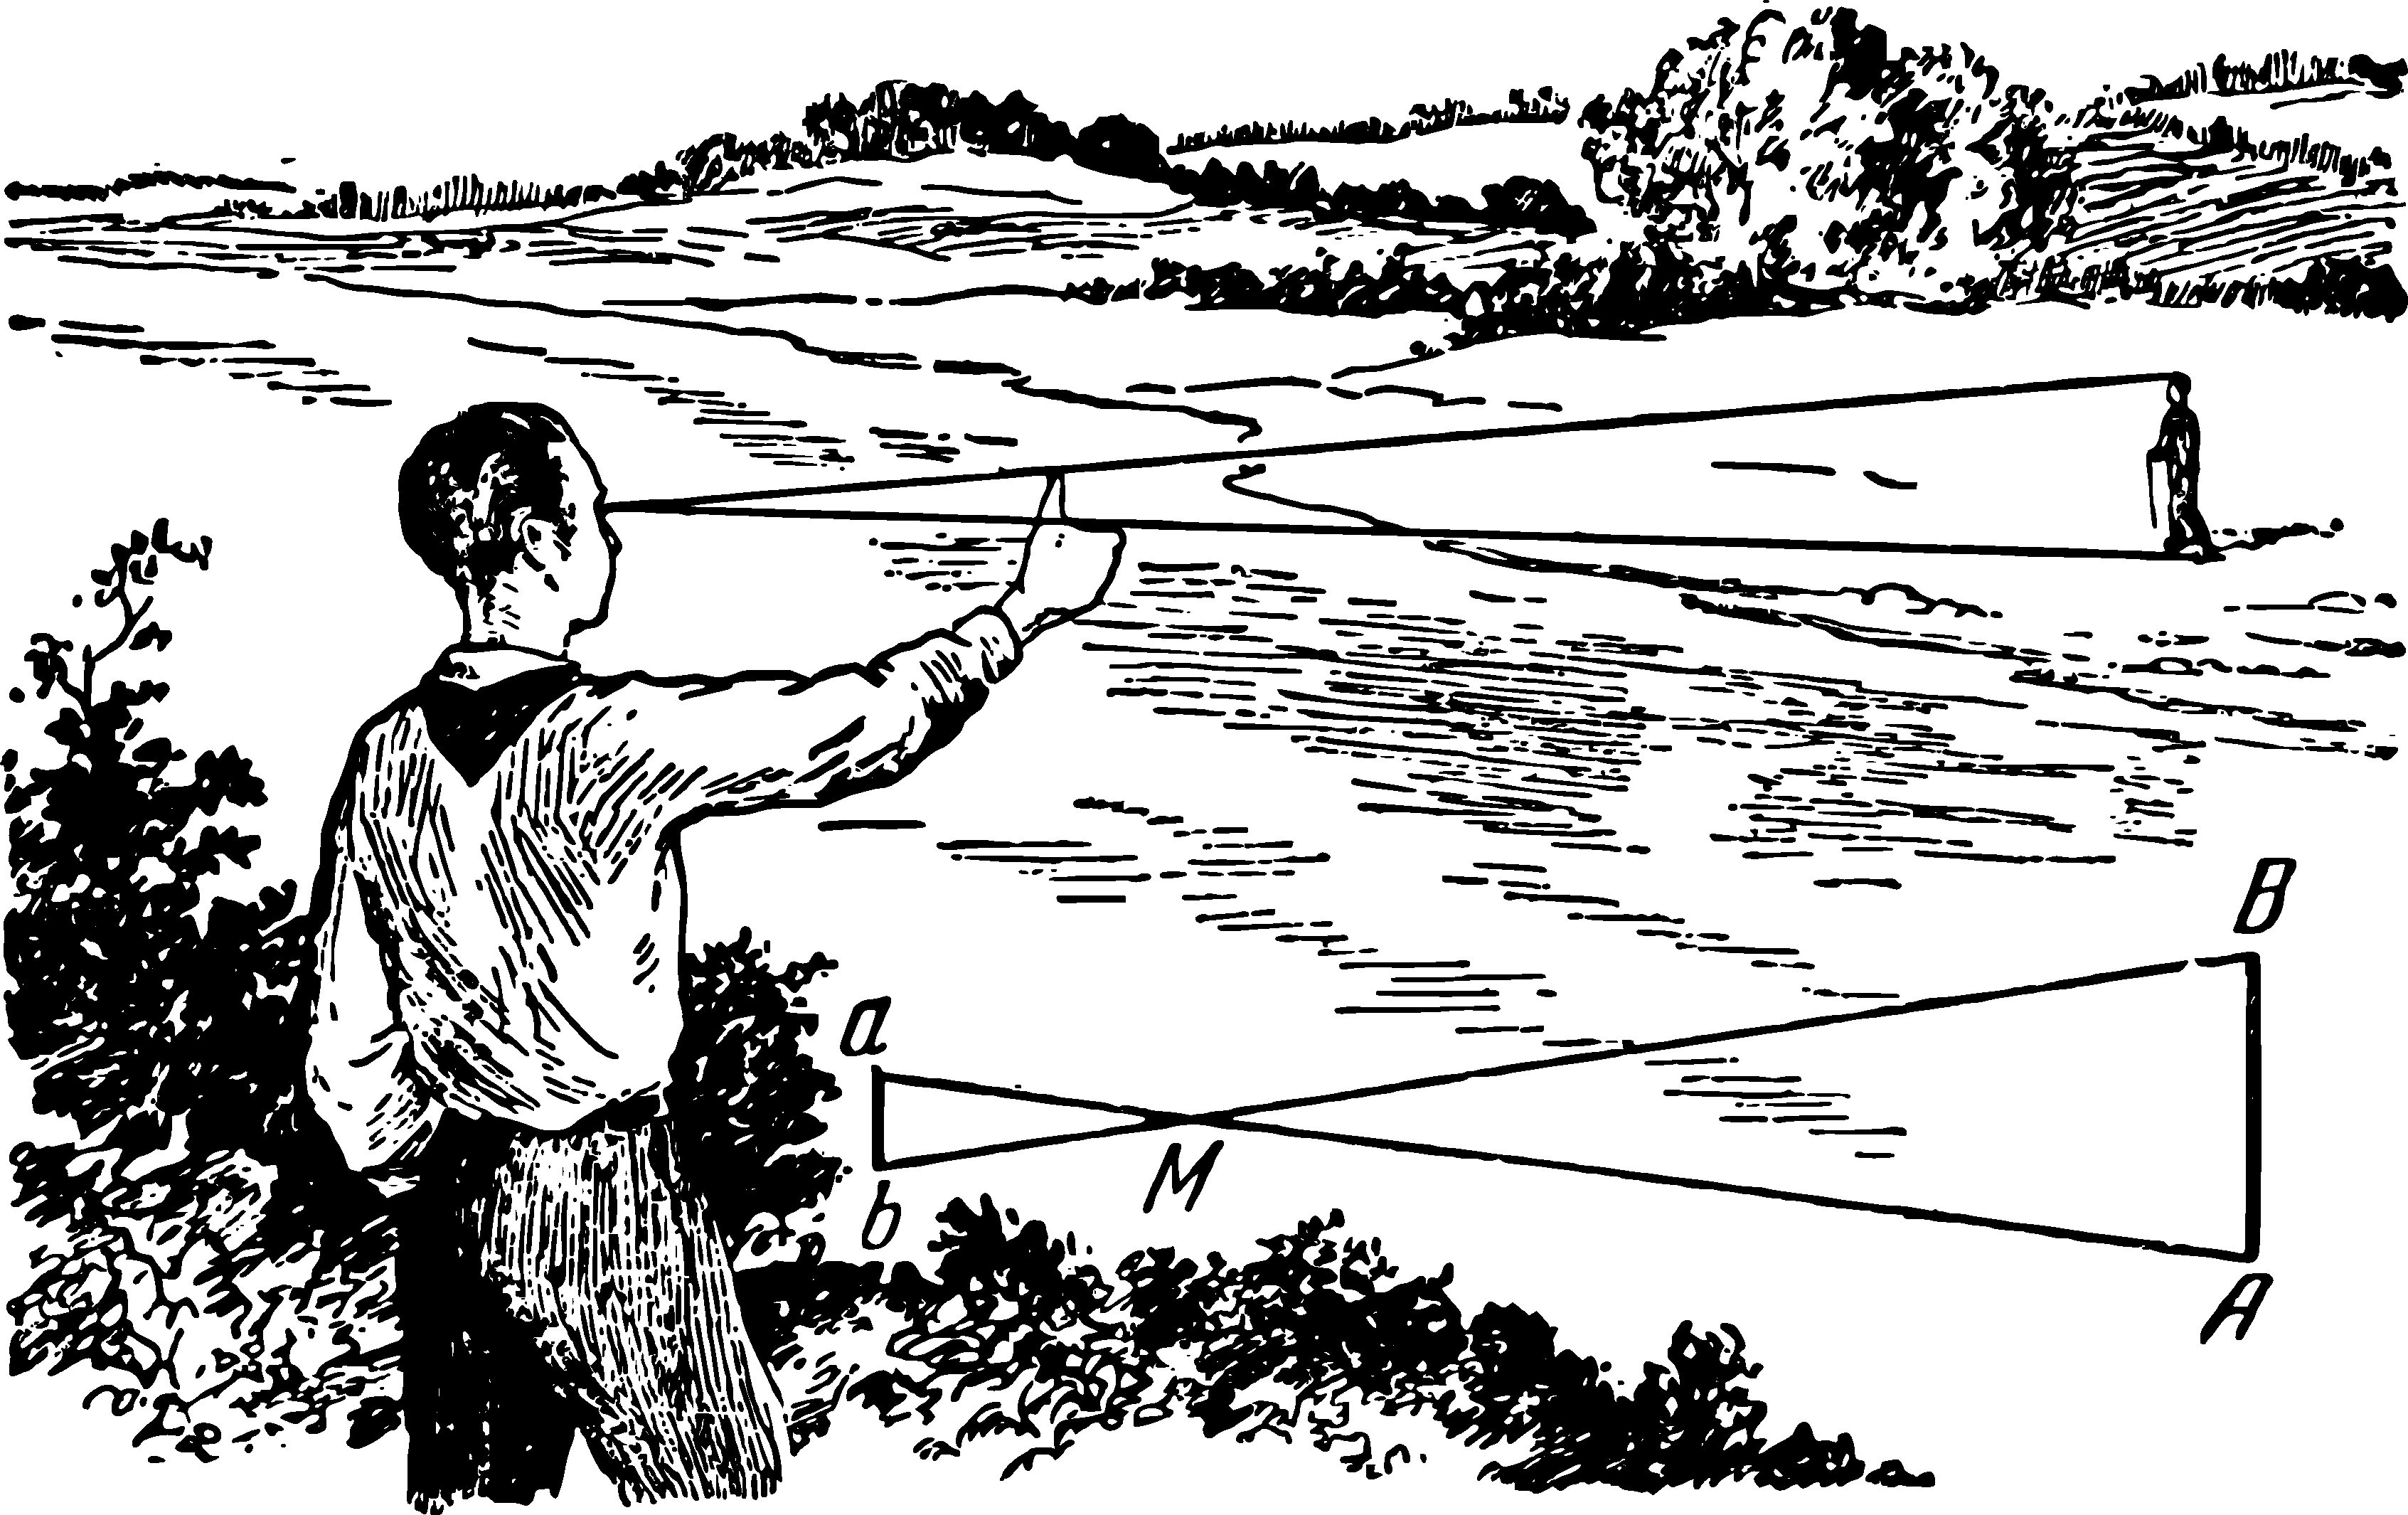
\includegraphics[width=0.9\textwidth]{figures/ch-02/fig-036.pdf}
\sidecaption{How to determine the distance to a pedestrian walking on the other side of the river.\label{fig-036}}
\end{figure}


\ans You don't have any instruments, but you have eyes and hands -- that's enough. Extend your arm forward towards the pedestrian and look at the tip of your finger with one eye if the pedestrian is moving towards your right hand, and with the other eye if they're moving towards your left hand. At the moment when the distant pedestrian is covered by your finger (see \figr{fig-036}), close the eye that was looking and open the other: the pedestrian will appear to you as if they've moved backward. Count how many steps they take before they align again with your finger. You'll get all the data needed for an approximate determination of the distance. Let's explain how to use them.

Suppose in \figr{fig-036} (inset), your eyes are marked as $a$ and $b$, point $M$ is the tip of your finger extended, point $A$ is the initial position of the pedestrian, and $B$ is the final position. The triangles $abM$ and $ABM$ are similar (you should turn towards the pedestrian so that $ab$ is approximately parallel to their direction of movement). Therefore, $BM : bM = AB : ab$ -- is a proportion in which only one term, $BM$, is unknown, but all others can be directly determined. Indeed, $bM$ is the length of your extended arm, $ab$ is the distance between the pupils of your eyes, and $AB$ is measured in steps taken by the pedestrian (assuming an average step to be around 3/4 metres). Therefore, the unknown distance from you to the pedestrian on the opposite bank, $AB$, equals 
\begin{equation*}%
MB = AB \, \frac{bM}{ab}
\end{equation*}
For example, if the distance between your eye pupils $ab$ is \SI{6}{\centi\meter}, the length of $bM$ from the end of your extended arm to the eye is \SI{60}{\centi\meter}, and the pedestrian takes, say, 14 steps from $A$ to $B$, then their distance from you would be $MB = 14 \cdot 60/6 = 140$ steps, or 105 meters.

It's enough for you to measure in advance the distance between your eye pupils and $bM$ -- the distance from the eye to the end of your extended arm -- so that you can quickly determine the distance of inaccessible objects by remembering their ratio. On average, for most people, $bM/ab$ is around 10 with slight fluctuations. The difficulty will only be in somehow determining the distance $AB$. In our case, we used the steps of a distant person. But you can also use other references. For instance, if you're measuring the distance to a distant freight train, you can estimate $AB$ in comparison to the length of a freight car, which is usually known (7.6 meters between buffers). If you're determining the distance to a house, you can estimate $AB$ by comparing it to the width of a window, the length of a brick, etc.

The same method can be applied to determine the size of a distant object if its distance from the observer is known. For this purpose, you can also use other ``rangefinders'', which we will describe next.

\section{Simple Rangefinders}
\begin{marginfigure}[-2cm]%[h!]
\centering

\includegraphics[width=0.1\textwidth]{figures/ch-02/fig-037.pdf}
\sidecaption{The match is a rangefinder.\label{fig-037}}
\end{marginfigure}
In the first chapter, we described the simplest instrument for determining inaccessible heights -- the altimeter. Now, let's describe the simplest device for measuring inaccessible distances -- the `rangefinder.' The simplest rangefinder can be made from an ordinary matchstick. To do this, you just need to mark millimeter divisions on one of its sides, alternating between light and dark (see \figr{fig-037}).


You can use this primitive ``rangefinder'' to estimate the distance to a distant object only in those cases when the dimensions of that object are known to you (see \figr{fig-038}). However, more sophisticated rangefinders can also be used under the same condition. Suppose you see a person in the distance and set yourself the task of determining the distance to them. Here, the matchstick rangefinder can come in handy. Holding it in your outstretched arm and looking with one eye, you bring its free end into coincidence with the top of the distant figure. Then, slowly moving your thumbnail along the matchstick, you stop it at the point that projects onto the base of the human figure. All you have to do now is to find out, by bringing the matchstick closer to the eye, at which mark your thumbnail stopped -- and then you have all the data to solve the problem.

\begin{figure}[h!]
\centering
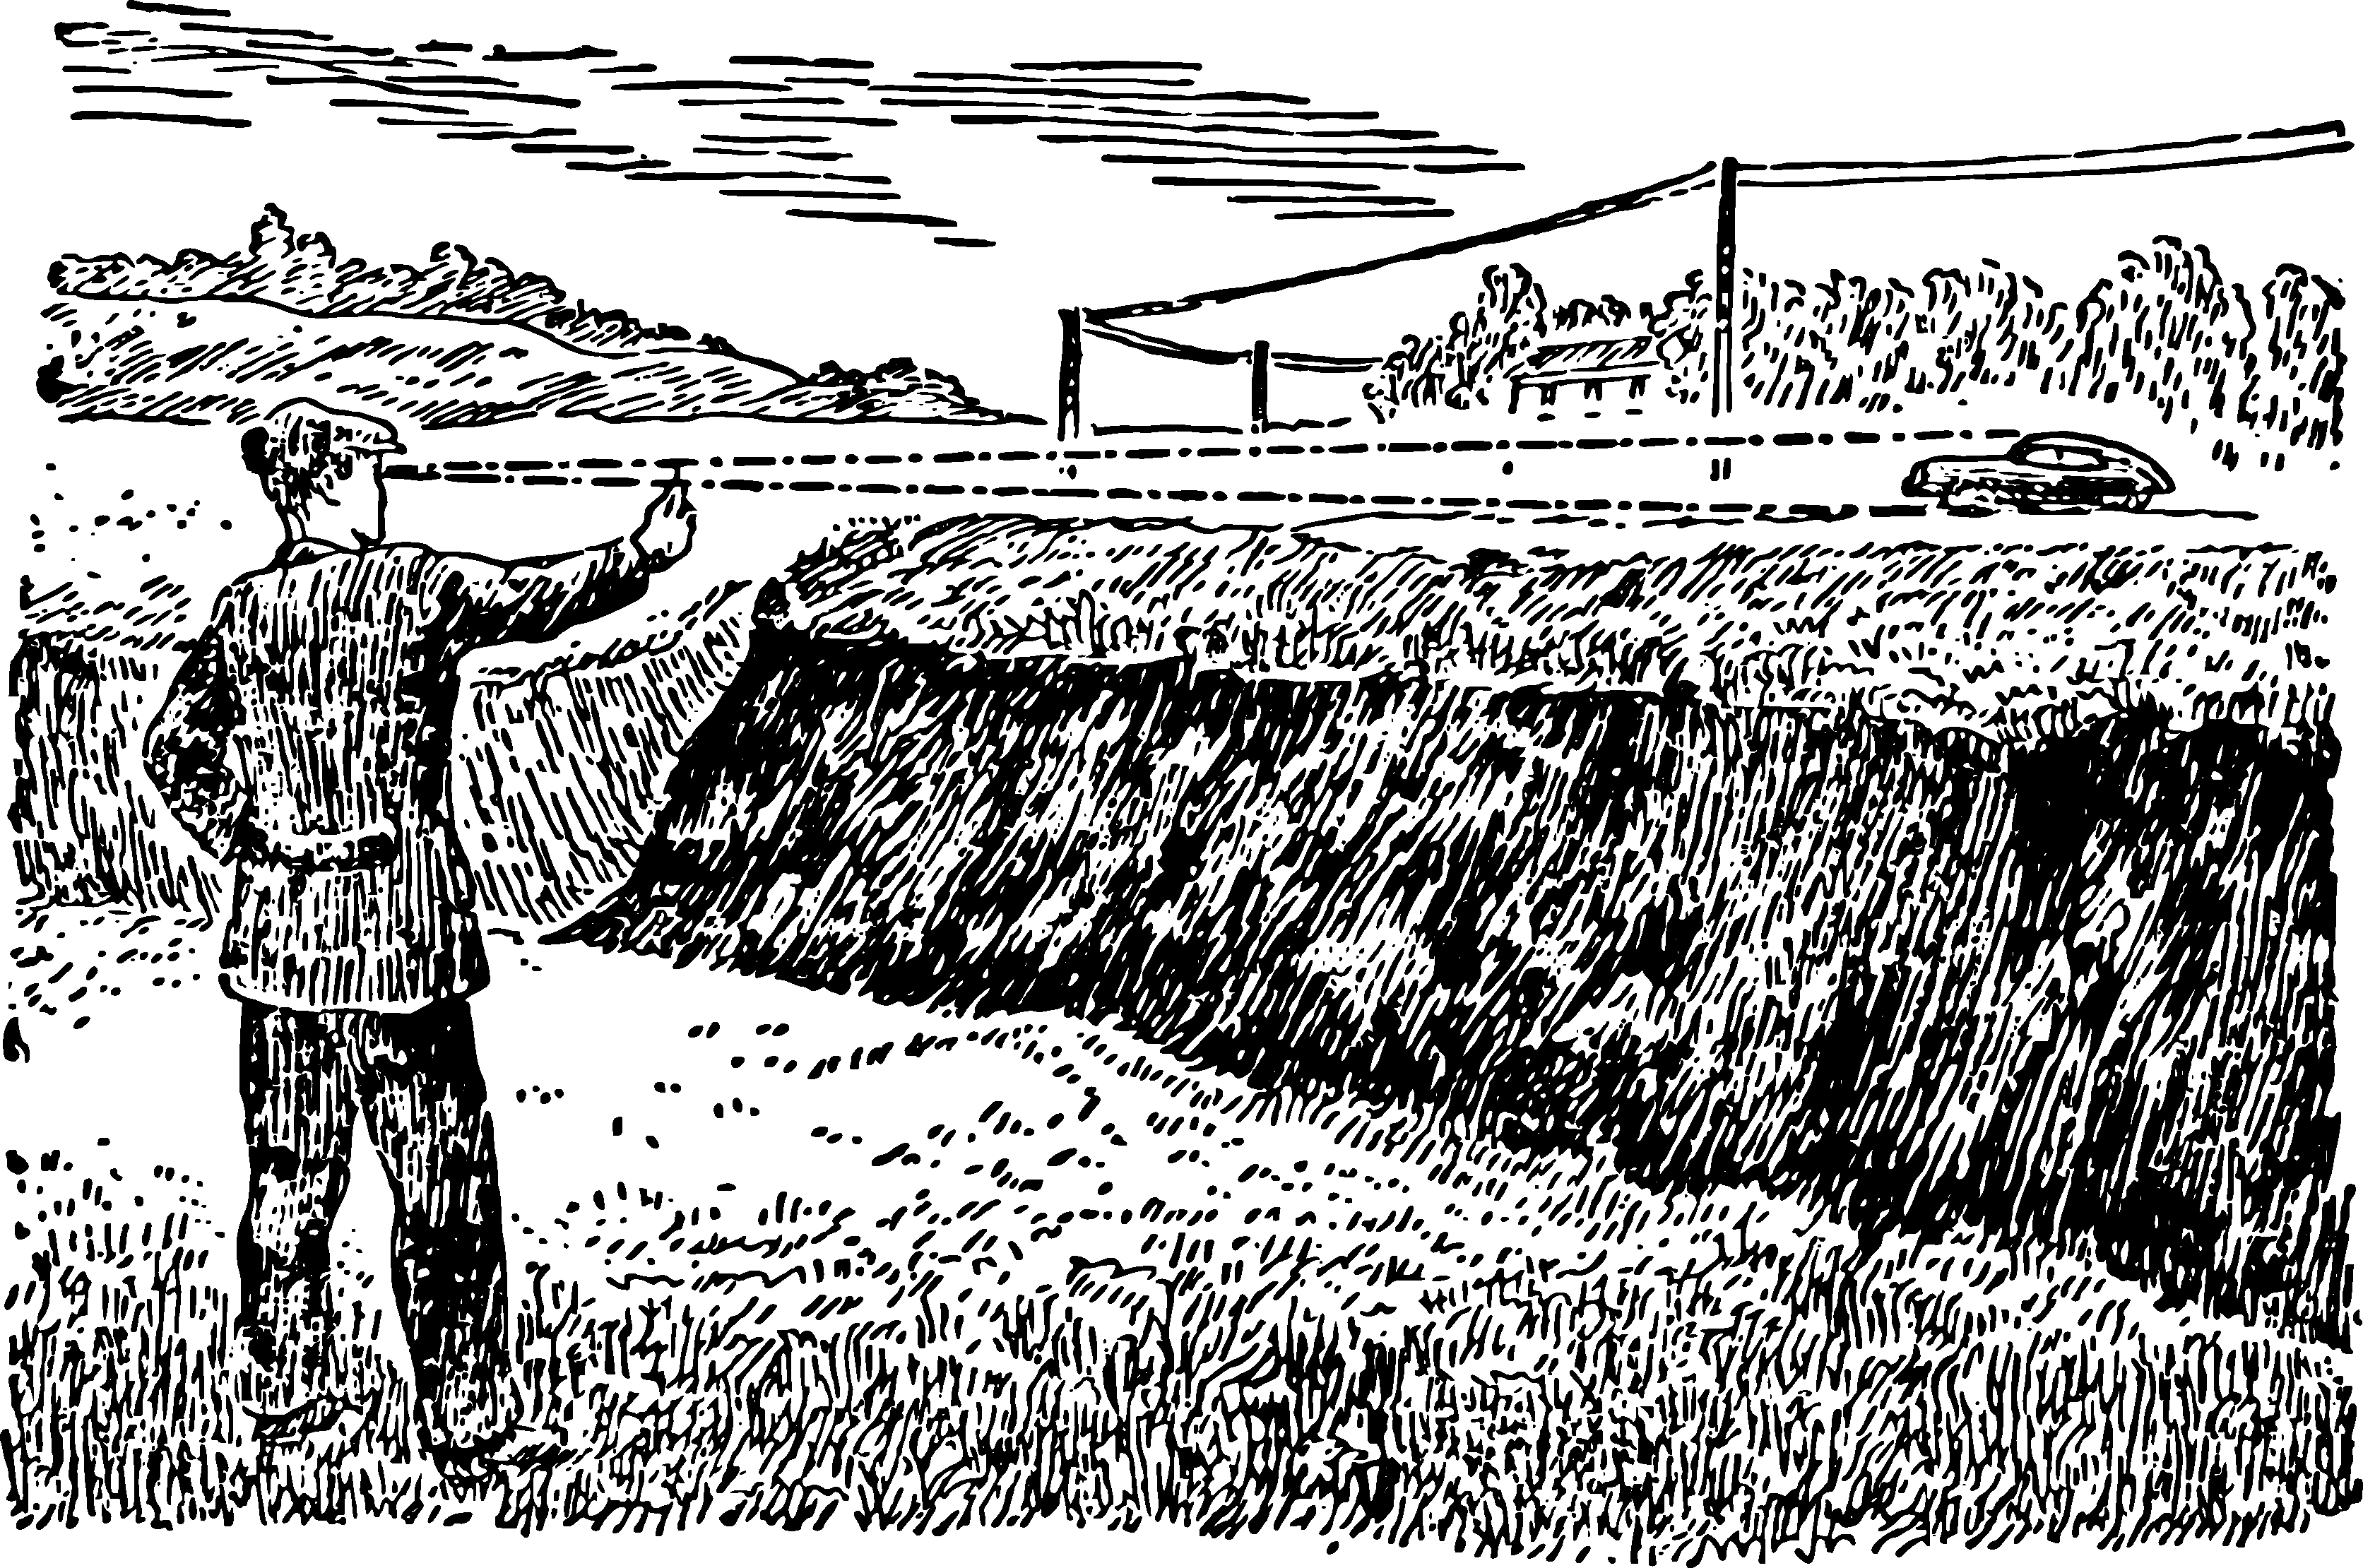
\includegraphics[width=\textwidth]{figures/ch-02/fig-038.pdf}
\sidecaption{The use of a rangefinder match to determine inaccessible distances.\label{fig-038}}
\end{figure}

You can easily verify the correctness of the proportion:
\begin{equation*}%
\frac{\text{desired distance}}{\begin{array}{c}\text{distance from the eye}\\ \text{to the matchstick}\end{array}} = \frac{\text{average height of a person}}{\begin{array}{c}\text{measured part}\\ \text{of the matchstick}\end{array}}
\end{equation*}
From here, it's easy to calculate the desired distance. For example, if the distance to the matchstick is \SI{60}{\centi\meter}, the height of the person is \SI{1.7}{\meter}, and the measured part of the matchstick is \SI{12}{\milli\meter}, then the determined distance would be:
\begin{equation*}%
60 \cdot \frac{1700}{12} = \SI{8500}{\centi\meter} = \SI{85}{\meter}.
\end{equation*}
To gain some skill in using this rangefinder, measure the height of someone from your group and, asking them to move away a certain distance, try to determine how many steps they took away from you.

With the same method, you can determine the distance to a rider (average height \SI{2.2}{\meter}), a cyclist (wheel diameter \SI{75}{\centi\meter}), a telegraph pole along the railway track (height \SI{8}{\meter}), vertical distance between adjacent insulators (\SI{90}{\centi\meter}), to a train, a brick house, and similar objects whose dimensions can be estimated with sufficient accuracy. There can be quite a few such cases during excursions.

\begin{marginfigure}%[-2cm]%[h!]
\centering
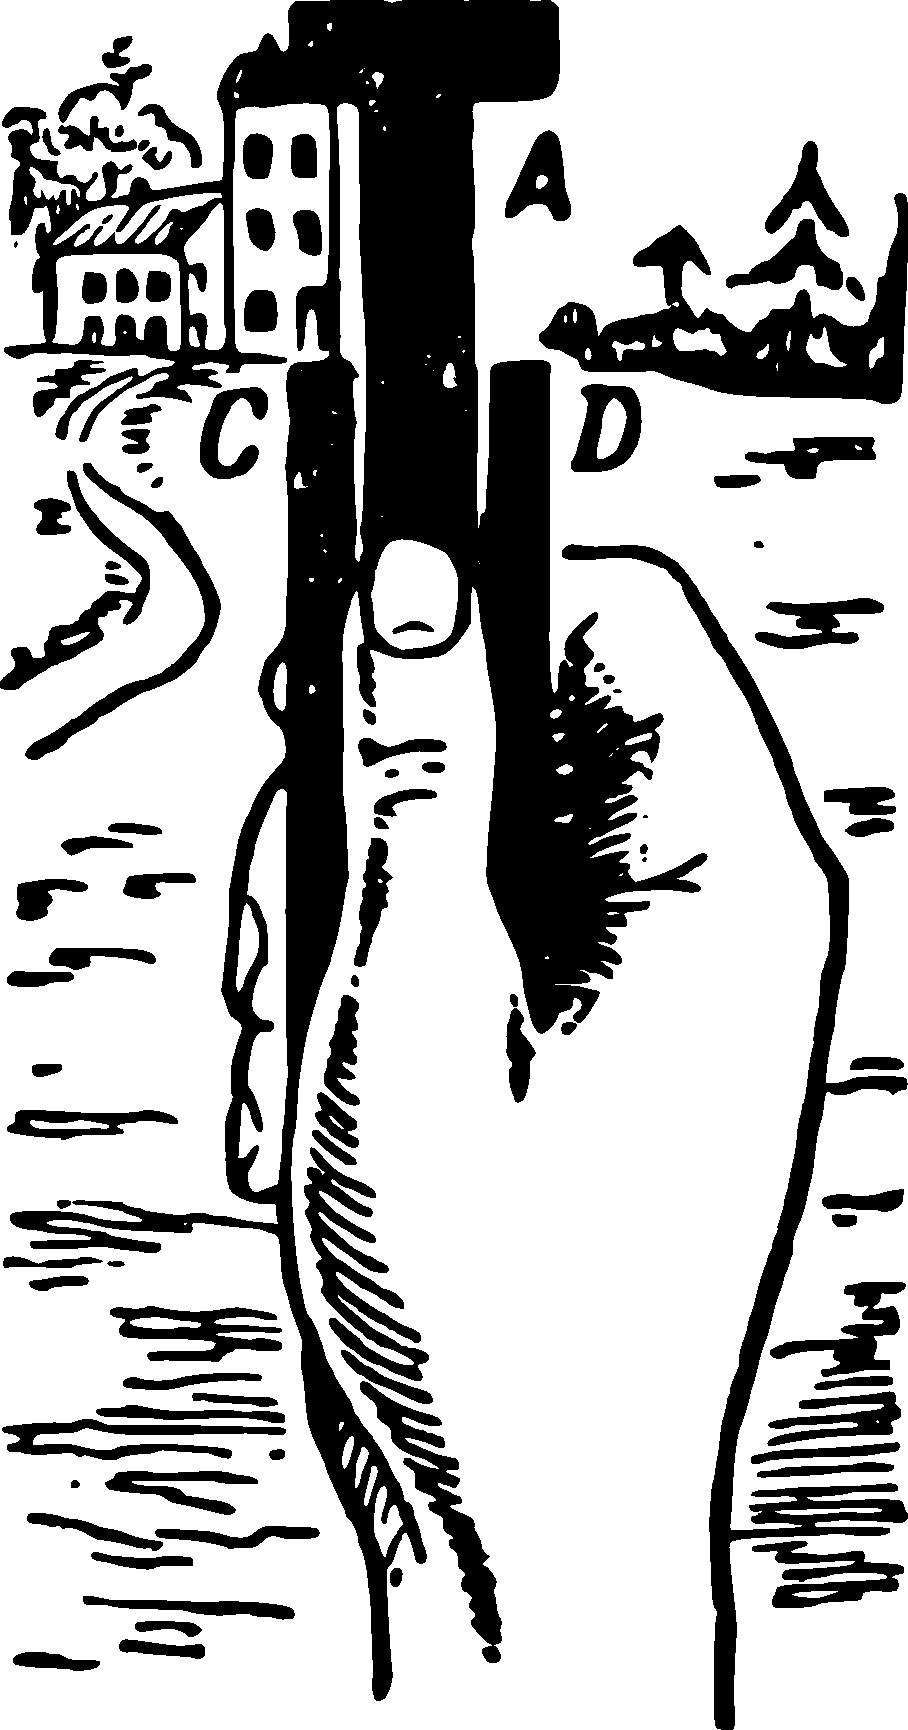
\includegraphics[width=0.8\textwidth]{figures/ch-02/fig-039.pdf}
\sidecaption{The retractable rangefinder in action.\label{fig-039}}
\end{marginfigure}

For those skilled in crafting, making a more convenient device of the same type, intended for estimating distances based on the size of a distant human figure, won't be much trouble.

\begin{marginfigure}%[-2cm]%[h!]
\centering
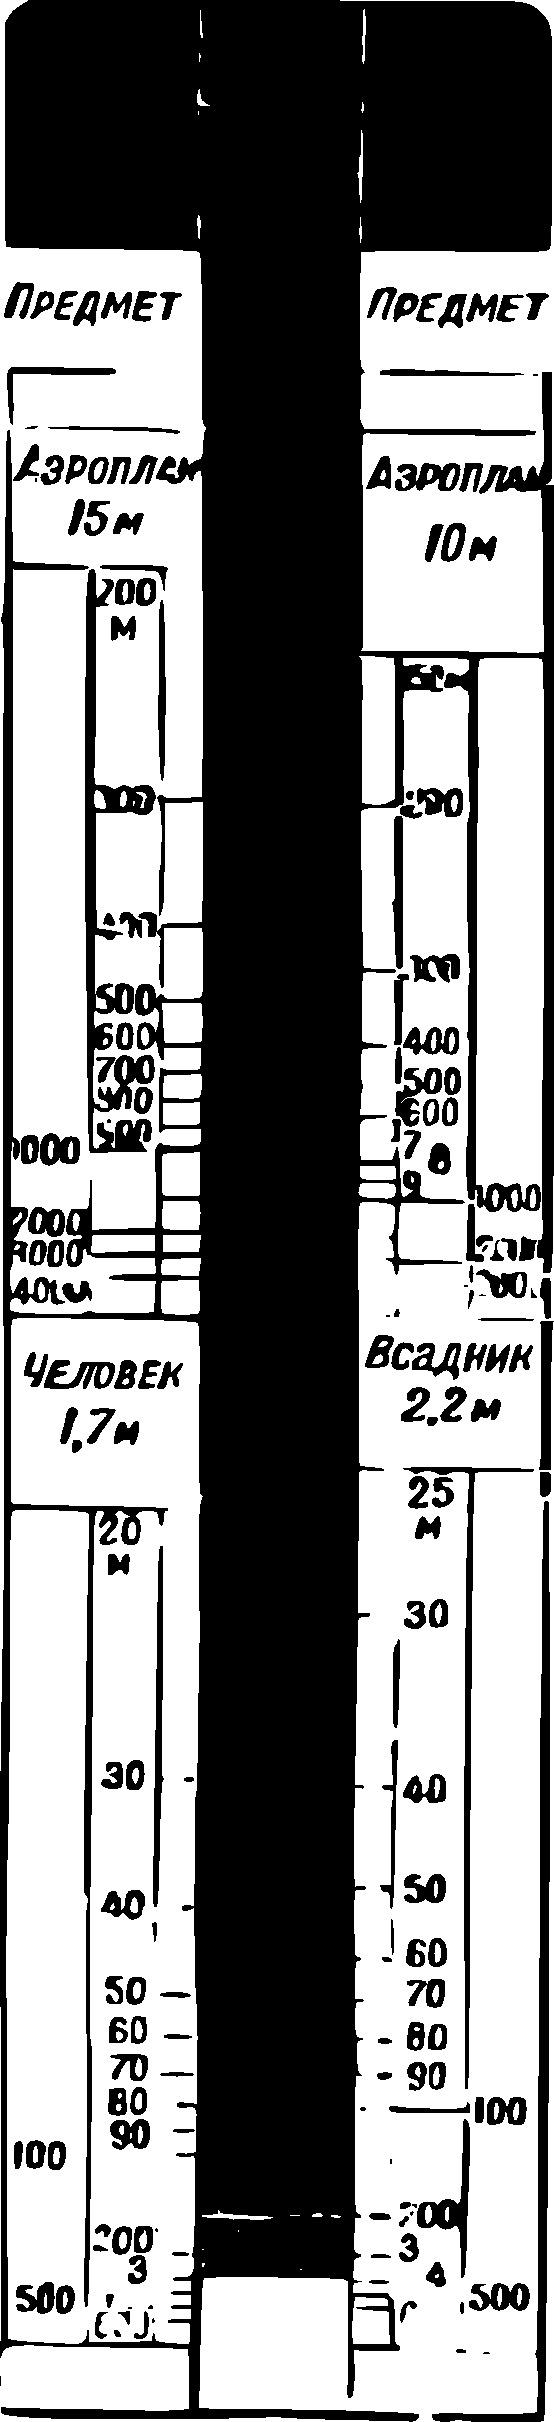
\includegraphics[width=0.6\textwidth]{figures/ch-02/fig-040.pdf}
\sidecaption{The design of the retractable rangefinder.\label{fig-040}}
\end{marginfigure}

The device is clear in \figr{fig-039} and \figr{fig-040}. The observed object is placed precisely in the gap $A$, formed when the extension part of the device is raised. The size of the gap can be conveniently determined by the divisions on the part $C$ and $D$ of the board. To avoid the need for any calculations, you can directly mark on strip $C$ the distances corresponding to the divisions if the observed object is a human figure (the device for measuring the distance of the outstretched arm). On the right strip $D$, you can mark distances, pre-calculated for cases where a rider is observed (\SI{2.2}{\meter}). For telegraph poles (height \SI{8}{\meter}), planes with a wingspan of \SI{15}{\meter}, and other larger objects, you can use the upper, free parts of strips $C$ and $D.$ Then the device will look like the one presented in \figr{fig-040}.





Of course, the accuracy of such distance estimation is low. It's just an estimate, not a measurement. In the example discussed earlier, where the distance to the human figure was estimated at \SI{85}{\meter}, an error of \SI{1}{\milli\meter} in measuring the matchstick portion would result in a deviation of \SI{7}{\meter} (1/12 out of 85). But if the person stood four times farther away, and we measured only \SI{3}{\milli\meter} on the matchstick, then an error of even 1/2 mm would cause a change in the result by \SI{57}{\meter}. Therefore, our example is reliable only for relatively short distances -- in the range of 100--200 m. When estimating larger distances, it's necessary to choose larger objects.


\section{The energy of the river}
\label{sec-2.6}

\begin{quote}
\emph{You know the edge where everything breathes abundance,\\
Where rivers flow purer than silver, \\
Where the steppe breeze sways the feather grass, \\
Where villages are nestled in cherry orchards.}\\[-10pt]
\flushright{\emph{A.K. Tolstoy}}
\end{quote}


A river, the length of which is no more than 100 km, is considered small. Do you know how many such small rivers there are in the USSR? A lot - 48 thousand!

If these rivers were stretched into a single line, it would result in a ribbon \SI{13800000}{\kilo\meter} long. With such a ribbon, you could encircle the Earth at the equator thirty times (the length of the equator is approximately \SI{40009}{\kilo\meter}).

The flow of these rivers is leisurely, but it conceals an inexhaustible supply of energy within it. Specialists believe that if the hidden potential of all the small rivers flowing through our homeland were combined, an impressive number would be obtained -- 34 million kilowatts! This gifted energy needs to be widely utilised for electrifying the economy of settlements located near rivers.

\begin{quote}
\emph{Let the river flow freely,\\
If the plan says so,\\
A dam with a stone ridge across all depths\\
Will block the way forever.}\\[-10pt]
\flushright{\emph{S. Shchipachev}}
\end{quote}

You know that this is achieved through hydroelectric power stations (HPS), and you can show a lot of initiative and provide real assistance in preparing for the construction of small HPS. Indeed, the builders of HPS will be interested in everything related to the river regime: its width and flow rate (``water flow''), the area of the cross-section of the riverbed (``active section''), and what water head the banks allow. And all this can be measured with available means and represents a relatively simple geometric problem.

We will now proceed to solving this problem.

But first, let's present here a practical advice from specialists, engineers V. Yarosh and I. Fedorov, regarding the selection of a suitable location on the river for the construction of a future dam.

They recommend building a small hydroelectric power station with a capacity of 15-20 kilowatts ``no further than 5 km from the village.''

``The dam of an HPS should be built no closer than 10-15 km and not farther than 20-40 km from the source of the river because moving away from the source entails the costly reinforcement of the dam, which is caused by a large influx of water. If the dam is located closer than 10-15 km from the source, due to the small water flow and insufficient head, the hydroelectric power station will not be able to provide the necessary power. The chosen stretch of the river should not be abundant in great depths, which also increases the cost of construction, requiring a heavy foundation.''

\section{The Flow Rate}
\label{sec-2.7}
\begin{quote}
\emph{Between village and mountain grove,\\
Winds a river like a bright ribbon.}\\[-10pt]
\flushright{\emph{A. Fet}}
\end{quote}

How much water flows in such a river in a day? It's easy to calculate if you first measure the speed of the water flow in the river. The measurement is performed by two people. One person holds a watch, the other holds some noticeable float, for example, a half-empty bottle with a flag. They choose a straight section of the river and place two stakes $A$ and $B$ along the bank at a distance, for example, \SI{10}{\meter} from each other (see \figr{fig-041}).

\begin{figure}[h!]
\centering
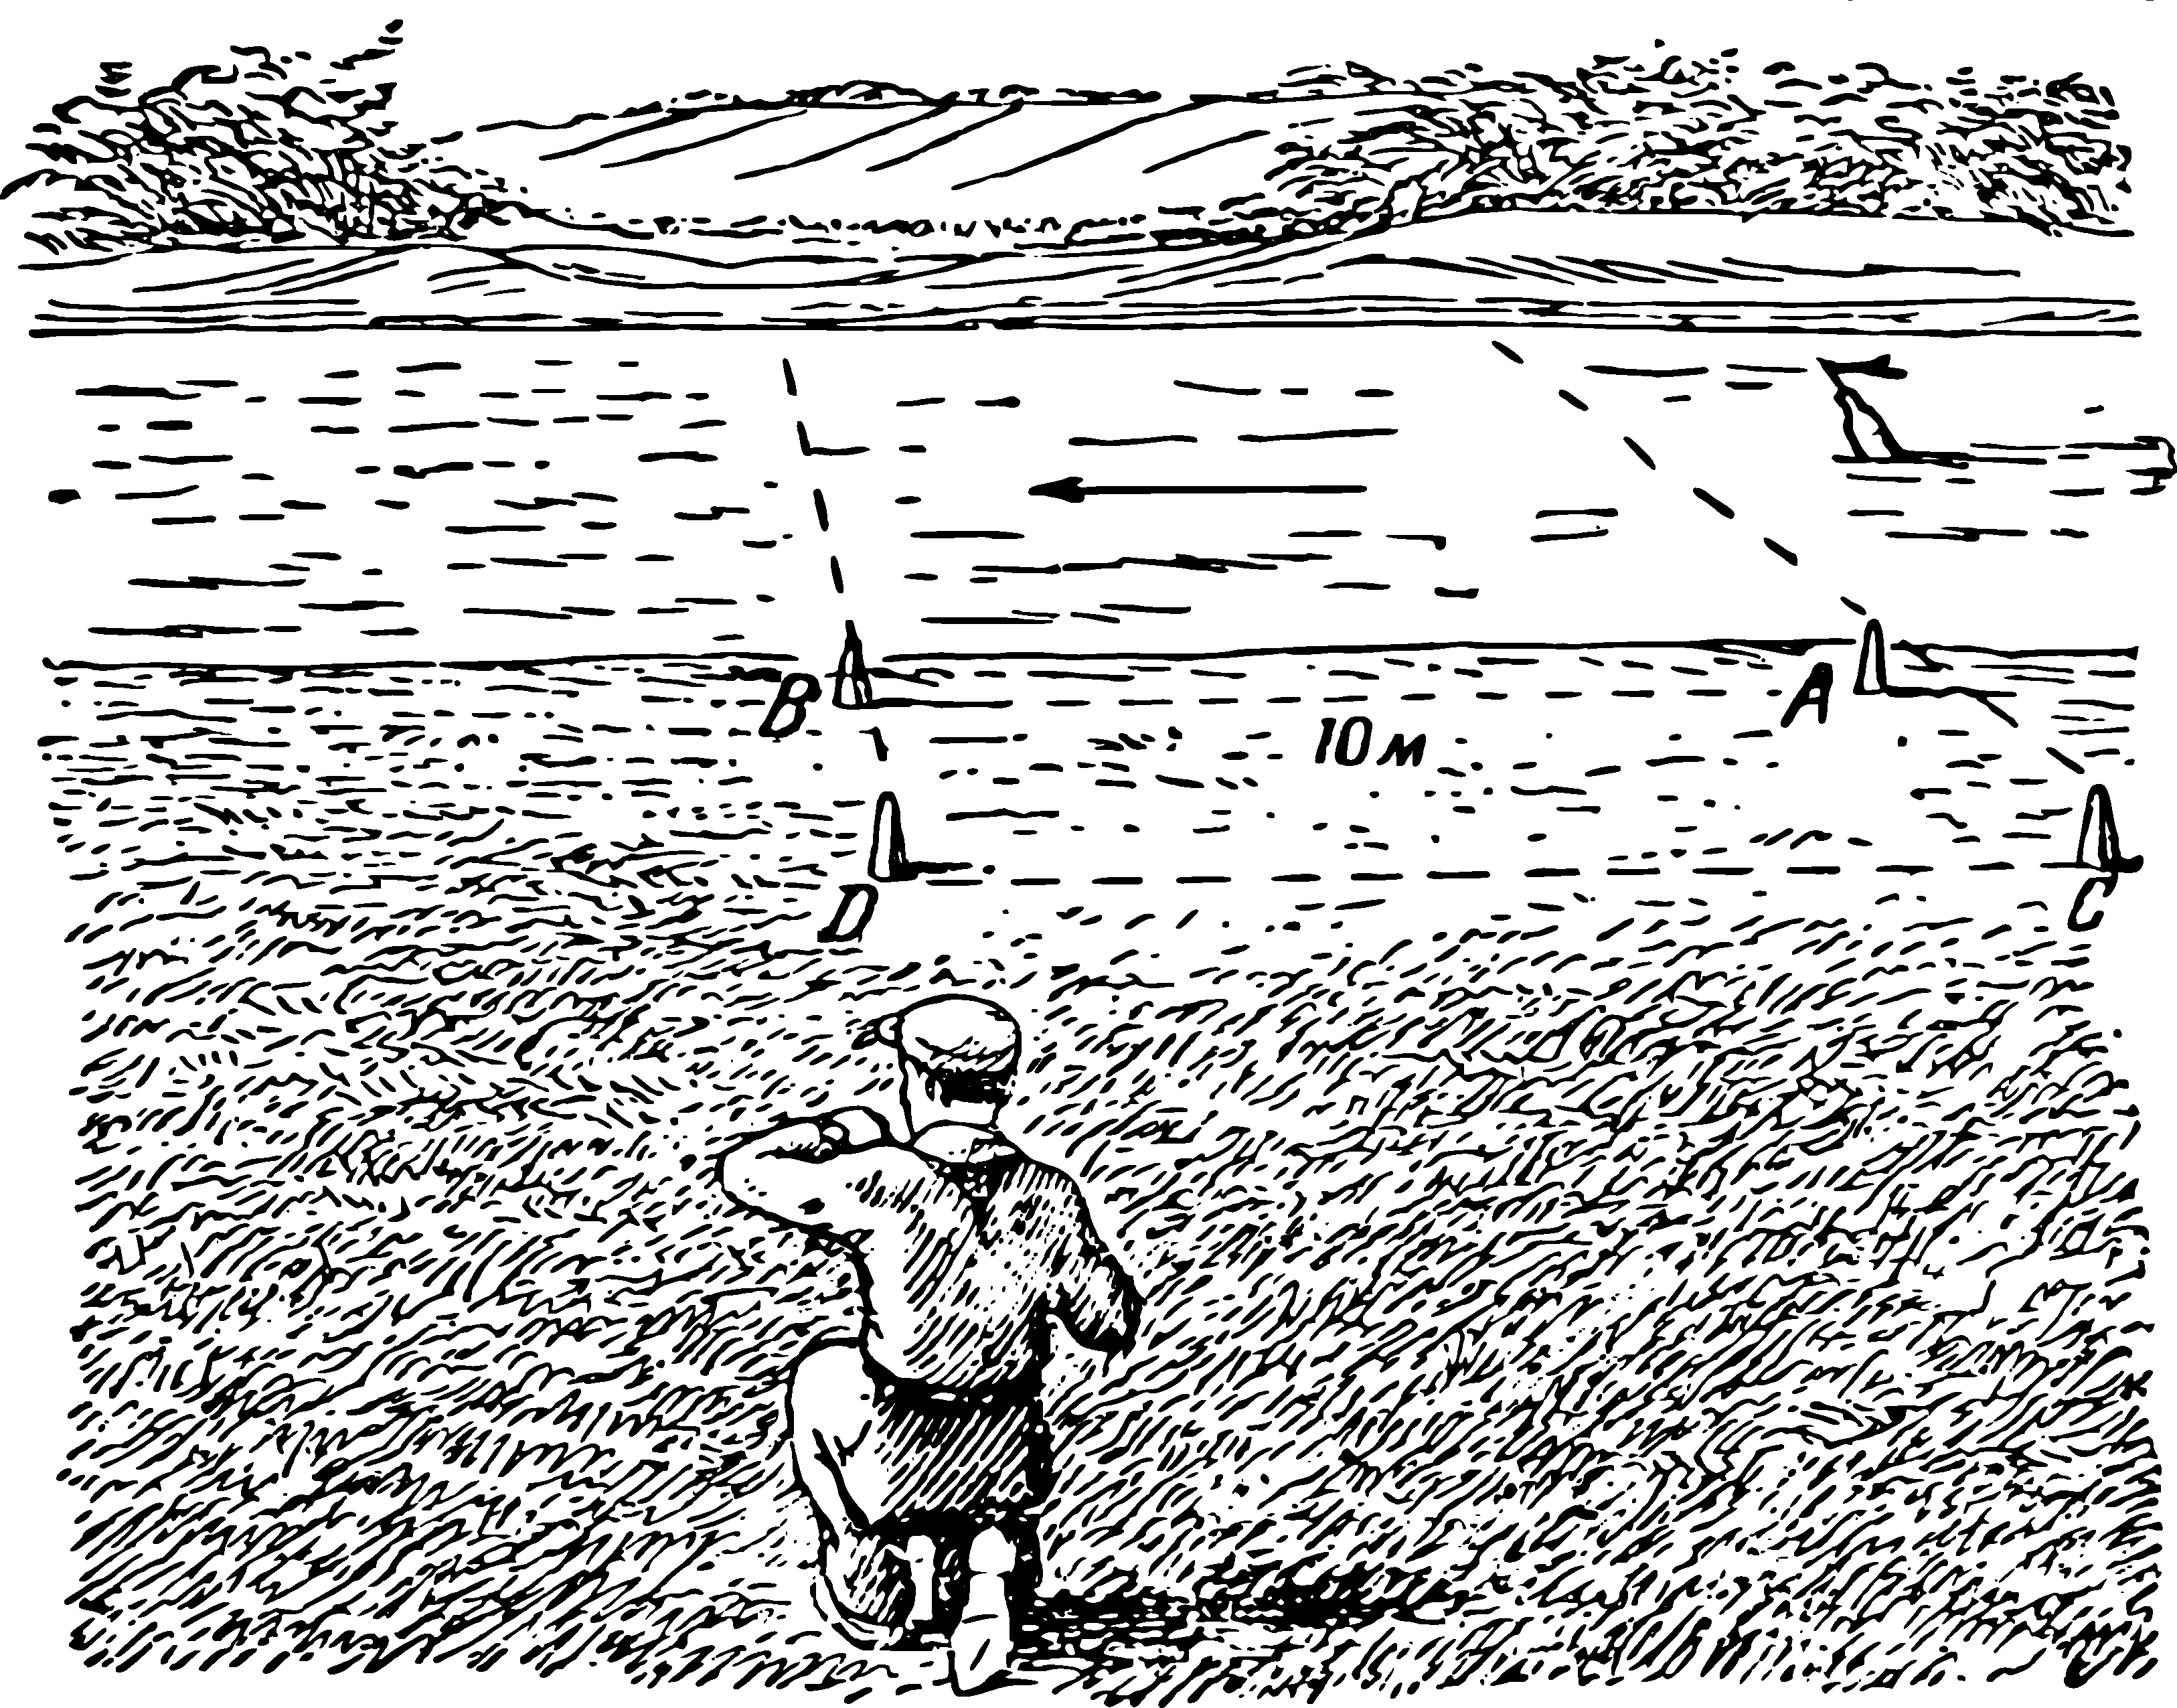
\includegraphics[width=0.9\textwidth]{figures/ch-02/fig-041.pdf}
\sidecaption{Measurement of the river flow velocity.\label{fig-041}}
\end{figure}

Two more stakes $C$ and $D$ are placed on lines perpendicular to $AB$. One of the participants in the measurement with the watch stands behind stake $D$. The other, with the float, goes a bit upstream of stake $A$, throws the float into the water, and then stands behind stake $C$. Both observers look along the directions $CA$ and $DB$ towards the water surface. At the moment when the float crosses the extension of the line $CA$, the first observer waves his hand. Upon this signal, the second observer starts the timer for the first time and then again when the float crosses the direction of $DB$.

Let's assume that the time difference is 20 seconds.

Then the speed of the water flow in the river is:
\begin{equation*}%
\frac{10}{20} = \SI{0.5}{\meter\per\second}.
\end{equation*}
Usually, the measurement is repeated about ten times\sidenote{Instead of throwing one float ten times, you can immediately throw 10 floats at some distance from each other.}, throwing the float into different points on the river surface. Then the obtained numbers are summed up and divided by the number of measurements. This gives the average speed of the surface layer of the river.

Deeper layers flow slower, and the average speed of the entire flow is approximately 4/5 times the surface speed. In our case, therefore, it's \SI{0.4}{\meter\per\second}.

You can determine the surface speed by another -- albeit less reliable -- method.

Sit in a boat and paddle \SI{1}{\kilo\meter} (measured along the shore) against the current, and then back -- with the current, trying to paddle with the same force all the time.

Let's say you paddled these \SI{1000}{\meter} against the current in 18 minutes, and with the current in 6 minutes. Denoting the desired speed of the river current as $x$, and the speed of your movement in still water as $y$, you form the equations:
\begin{equation*}%
\frac{1000}{y - x} = 18, \qand \frac{1000}{y + x} = 6.
\end{equation*}
Rearranging we get:
\begin{equation*}%
y + x = \frac{1000}{6}, \qand y - x = \frac{1000}{18}.
\end{equation*}
Solving for $x$, we get $2x = 110$, and $x = 55$. The speed of the water flow on the surface is 55 m per minute, and therefore, the average speed is about 5/6 \si{\meter\per\second}.


\section{How Much Water Flows In The River?}


To measure the amount of water flowing in a river, you can always determine the speed at which the water flows. The more challenging part of the preparatory work needed to calculate the quantity of flowing water is to determine the cross-sectional area of the water. To find the magnitude of this area, known as the ``live cross-section'' of the river, you need to make a drawing of this section. Such work is done as follows.

\textbf{First Method:} At the point where you measured the width of the river, you drive a stake into the ground on both banks, right at the water's edge. Then, with a companion, you get into a boat and row from one stake to the other, trying to keep a straight line connecting the stakes. An inexperienced rower will not be able to handle such a task, especially in a river with a fast current. Your companion must be a skilled rower; besides, a third participant in the work should stand on the bank, ensuring that the boat stays on the correct course and giving the rower signals indicating which way to turn when necessary. During the first crossing of the river, you only need to count how many strokes of the oars it took and from there figure out how many strokes move the boat 5 or 10 meters. Then, for the second crossing, armed with a sufficiently long rake with markings on it, you plunge the rake vertically to the bottom every 5-10 meters (measured by the number of oar strokes) and record the depth of the river at that point.

This method can only measure the live cross-section of a small river; for a wide, multi-water river, more complex methods are needed, which are performed by specialists. An amateur must choose a task that suits their modest measuring means.

\textbf{Second Method:} On a narrow and shallow river, you don't need a boat.

Between the stakes, you stretch a cord perpendicular to the current with marks or knots made on it every 1 or 2 meters, and by lowering a ruler to the bottom at each knot, you measure the depth of the riverbed. When all measurements are done, you first draw a millimeter paper or a grid paper sketch of the cross-section profile of the river. You will get a figure similar to the one shown in \figr{fig-042}. It is quite easy to determine the area of this figure since it can be divided into a series of trapezoids (where both bases and the height are known) and two side triangles, also with known base and height. If the scale of the drawing is 1:100, then the result will be obtained directly in square meters.

\begin{figure}[h!]
\centering
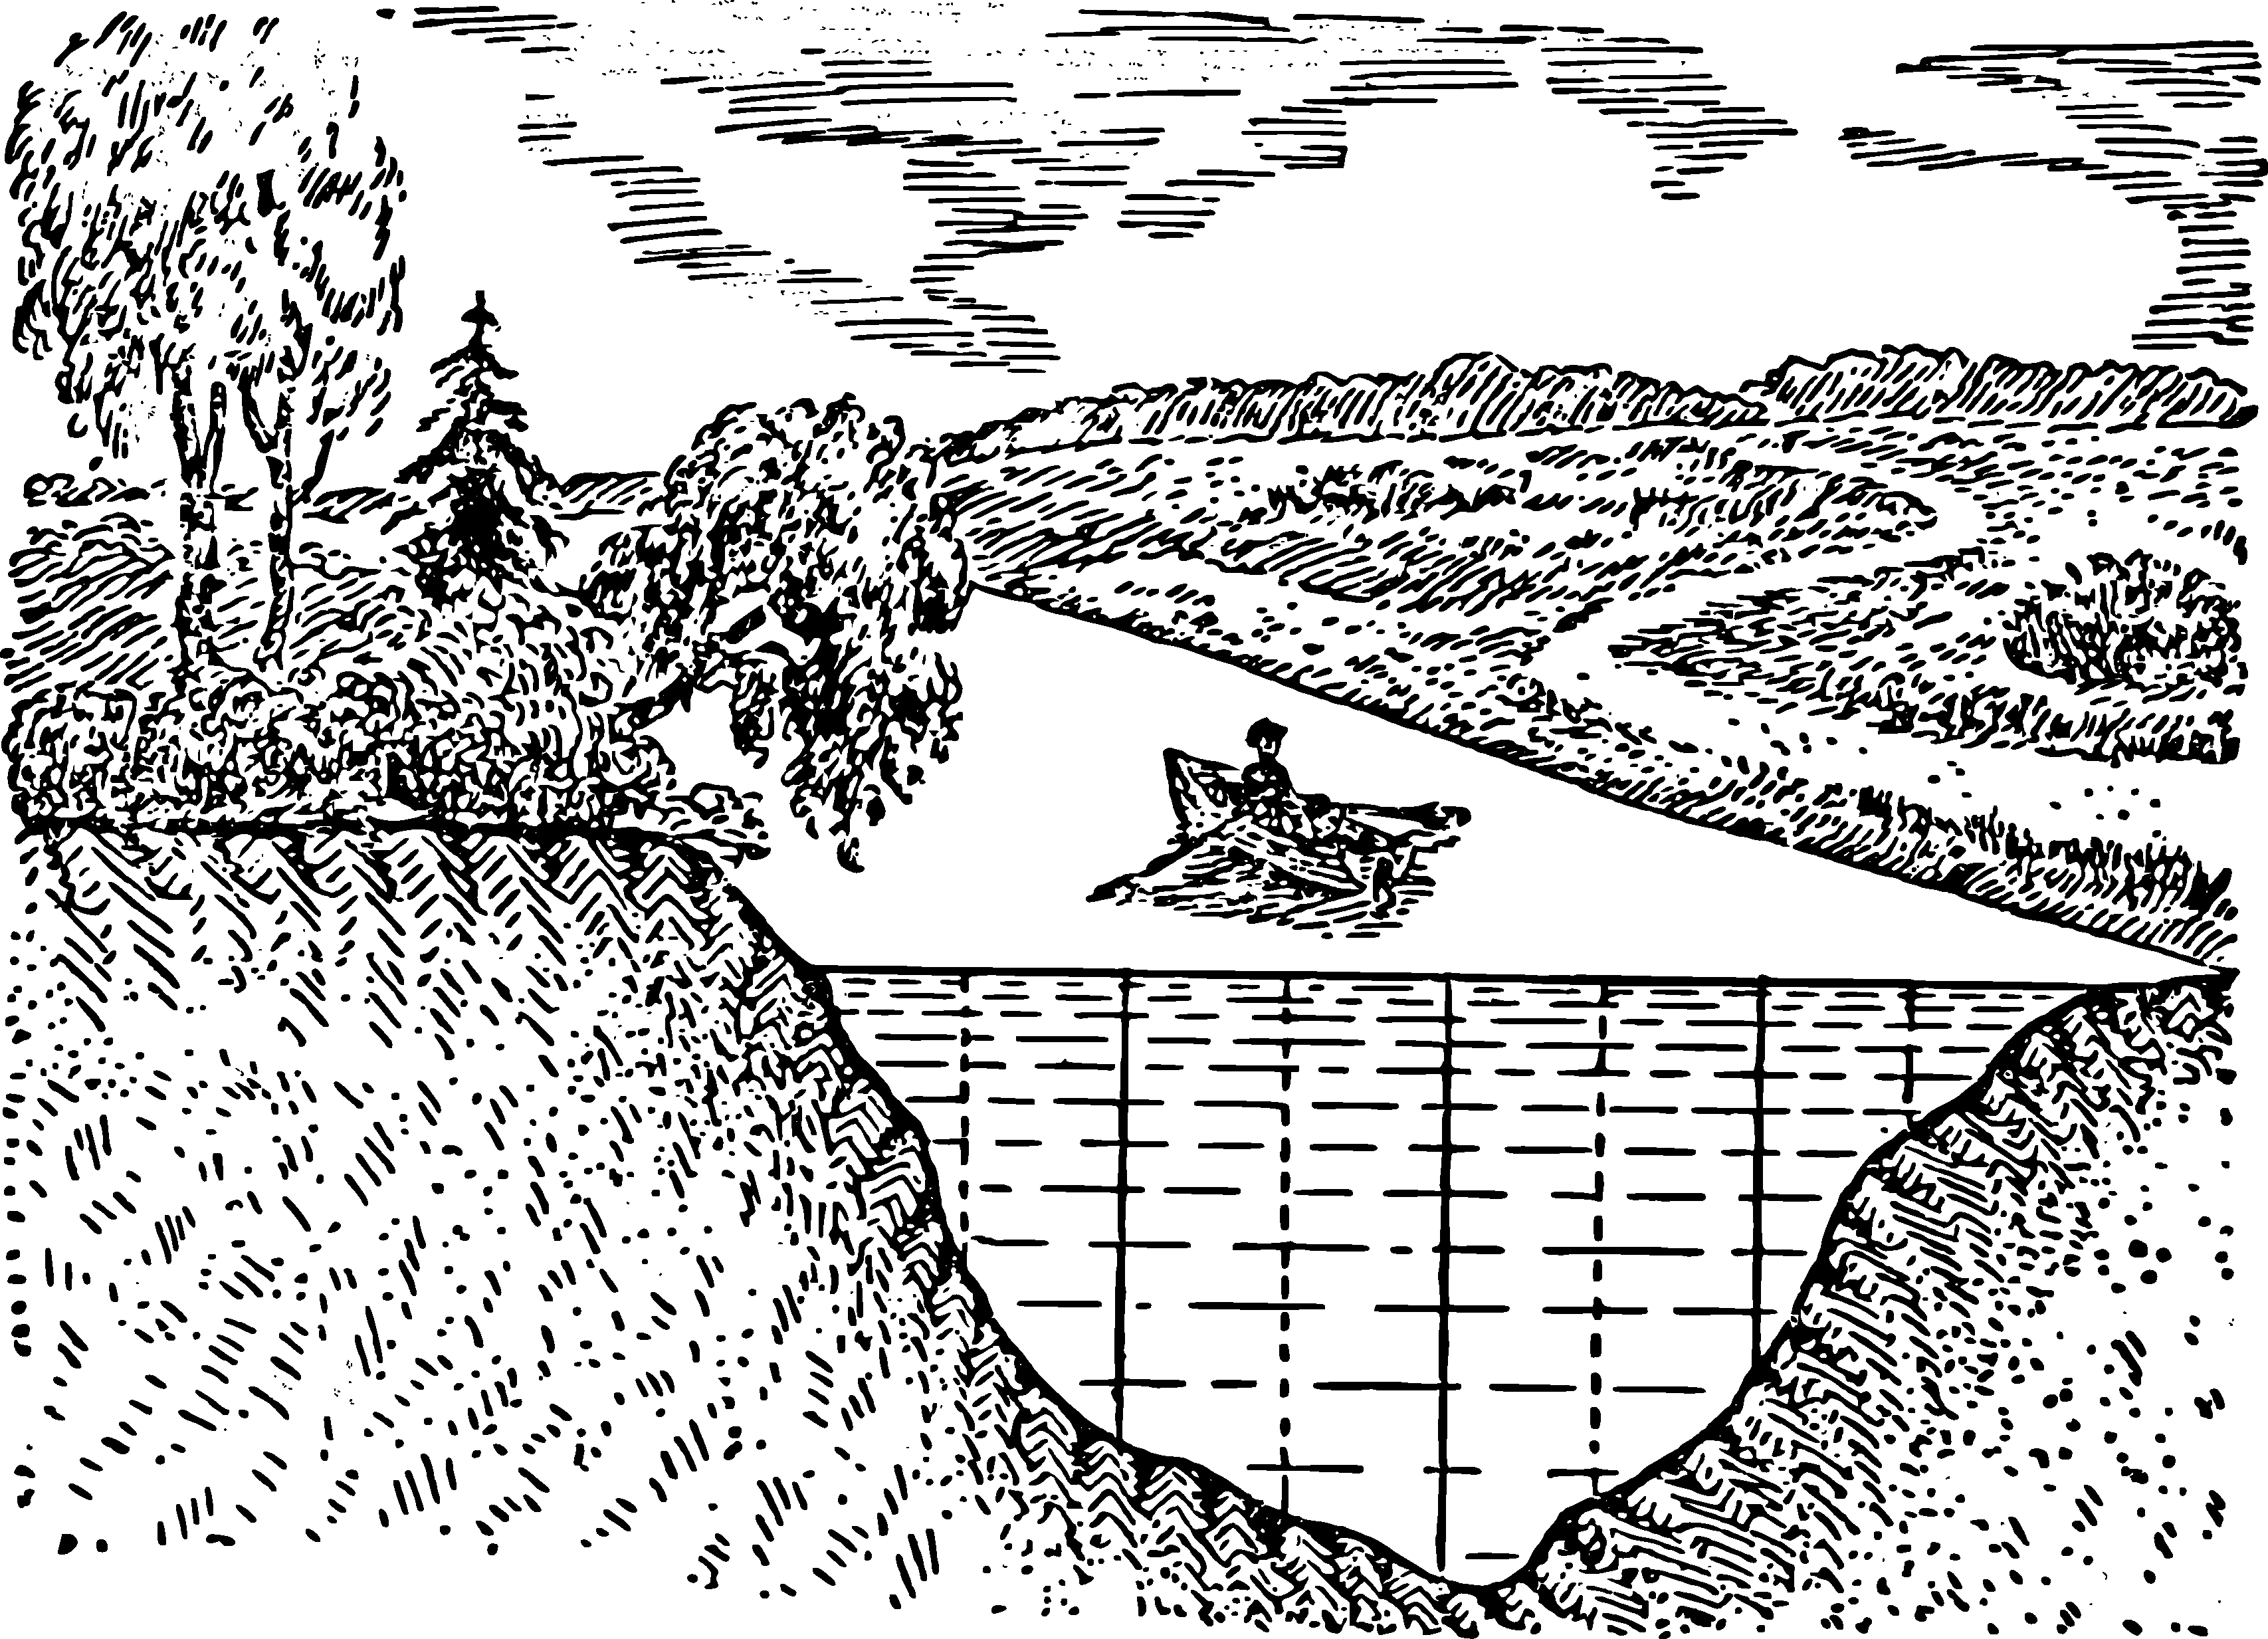
\includegraphics[width=0.9\textwidth]{figures/ch-02/fig-042.pdf}
\sidecaption{``Live Cross-Section'' of a River.\label{fig-042}}
\end{figure}

Now you have all the data needed to calculate the amount of flowing water. Obviously, through the live cross-section of the river, a volume of water equal to the volume of a prism is passing every second, where the cross-section serves as the base and the average second-by-second flow rate serves as the height. For example, if the average flow rate of water in the river is 0.4 meters per second, and the area of the live cross-section is, let's say, 3.5 square meters, then every second, through this section, there will be a transfer of

3.5 * 0.4 = 1.4 cubic meters of water,

or the same amount in tons. This amounts to 1.4 x 3600 = 5040 cubic meters per hour, and 5040 x 24 = 120960 cubic meters per day, which is over a hundred thousand cubic meters. And yet, a river with a wetted cross-section of 3.5 square meters is a small river; it could be, for example, 3.5 meters wide and 1 meter deep at a fordable point. But even it contains energy capable of transforming into mighty electricity. So how much water flows per day in a river like the Neva, through which 3300 cubic meters of water pass every second through its wetted cross-section! This is the 'average flow rate' of water in the Neva at Leningrad. The 'average flow rate' of water in the Dnieper at Kiev is 700 cubic meters.

Young explorers and future dam builders also need to determine the maximum head the banks can allow, i.e., the difference in water levels that the dam can create (Fig. 43). To do this, stakes are driven into the banks 5-10 meters away from the water, as usual, along a line perpendicular to the river's current. Then, moving along this line, small stakes are placed at points of characteristic bends in the banks (Fig. 44). Using rulers with markings, the elevation of one stake above the other and the distances between them are measured. Based on the measurement results, a profile of the banks is drawn similar to the profile of the riverbed. The bank profile can indicate the magnitude of the allowable head.

Suppose the water level can be raised by the dam by 2.5 meters. In this case, you can estimate the potential power of your future hydroelectric power plant.

For this, energy experts recommend multiplying 1.4 (the second-by-second flow rate of the river) by 2.5 (the water level height) and by 6 (the coefficient, which varies depending on energy losses in machines). The result will be in kilowatts. Thus,

1.4 x 2.5 x 6 = 21 kilowatts.

Since the river levels, and consequently the flow rates, vary throughout the year, it is necessary to calculate the value of the flow rate that is characteristic of the river for most of the year."

%\begin{center}
%
\includegraphics[width=0.3\textwidth]{figures/ch-02/fig-ch-02-tail.pdf}
%\end{center}



















% !TEX root = perelman-geometry.tex
%!TEX TS-program = pdflatex
%!TEX encoding = UTF-8 Unicode

\setchapterpreamble[o]{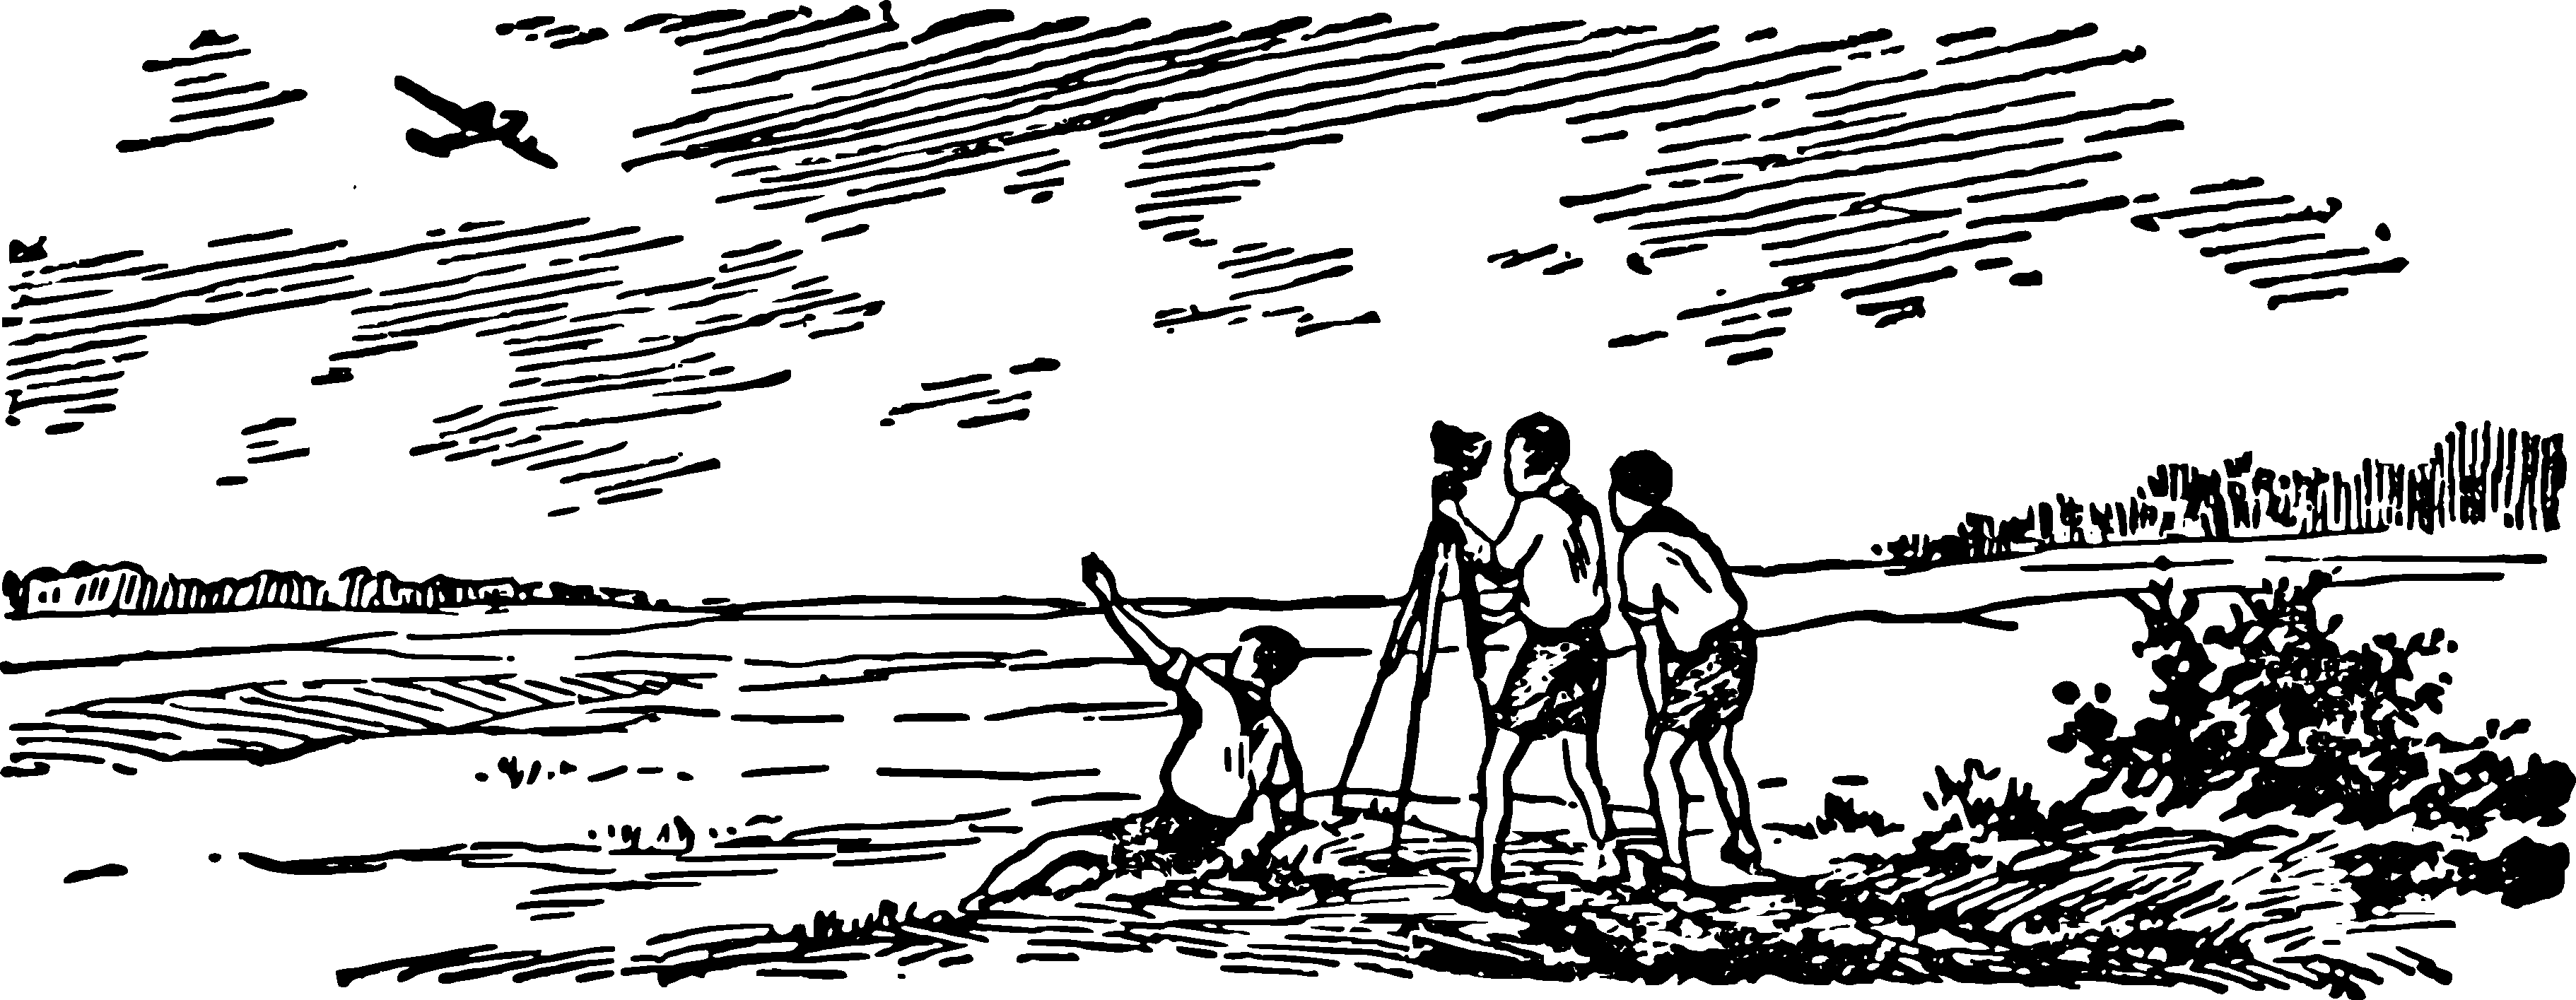
\includegraphics[width=1.2\textwidth]{figures/ch-03/fig-ch-03-head.pdf}\bigskip}

\chapter{Geometry In The Open Field}
\label{ch-03}

\section{Visible sizes of the Moon}
\label{sec-3.1}


What size does the full moon in the sky seem to you? Different people give quite different answers to this question.

Estimates like ``the size of a plate,'' ``the size of an apple,'' ``the size of a human face,'' and so on, are extremely vague, indefinite, indicating only that those answering do not understand the essence of the question.

The correct answer to such an apparently ordinary question can only be given by someone who clearly understands what exactly needs to be understood by the ``apparent'' or ``visible'' size of an object. Few suspect that here we are referring to the magnitude of a certain angle -- precisely the angle formed by two straight lines drawn to our eye from the extreme points of the object under consideration; this angle is called the ``angle of view'' or ``angular size of the object'' (\figr{fig-061}). 

\begin{figure}[h!]
\centering
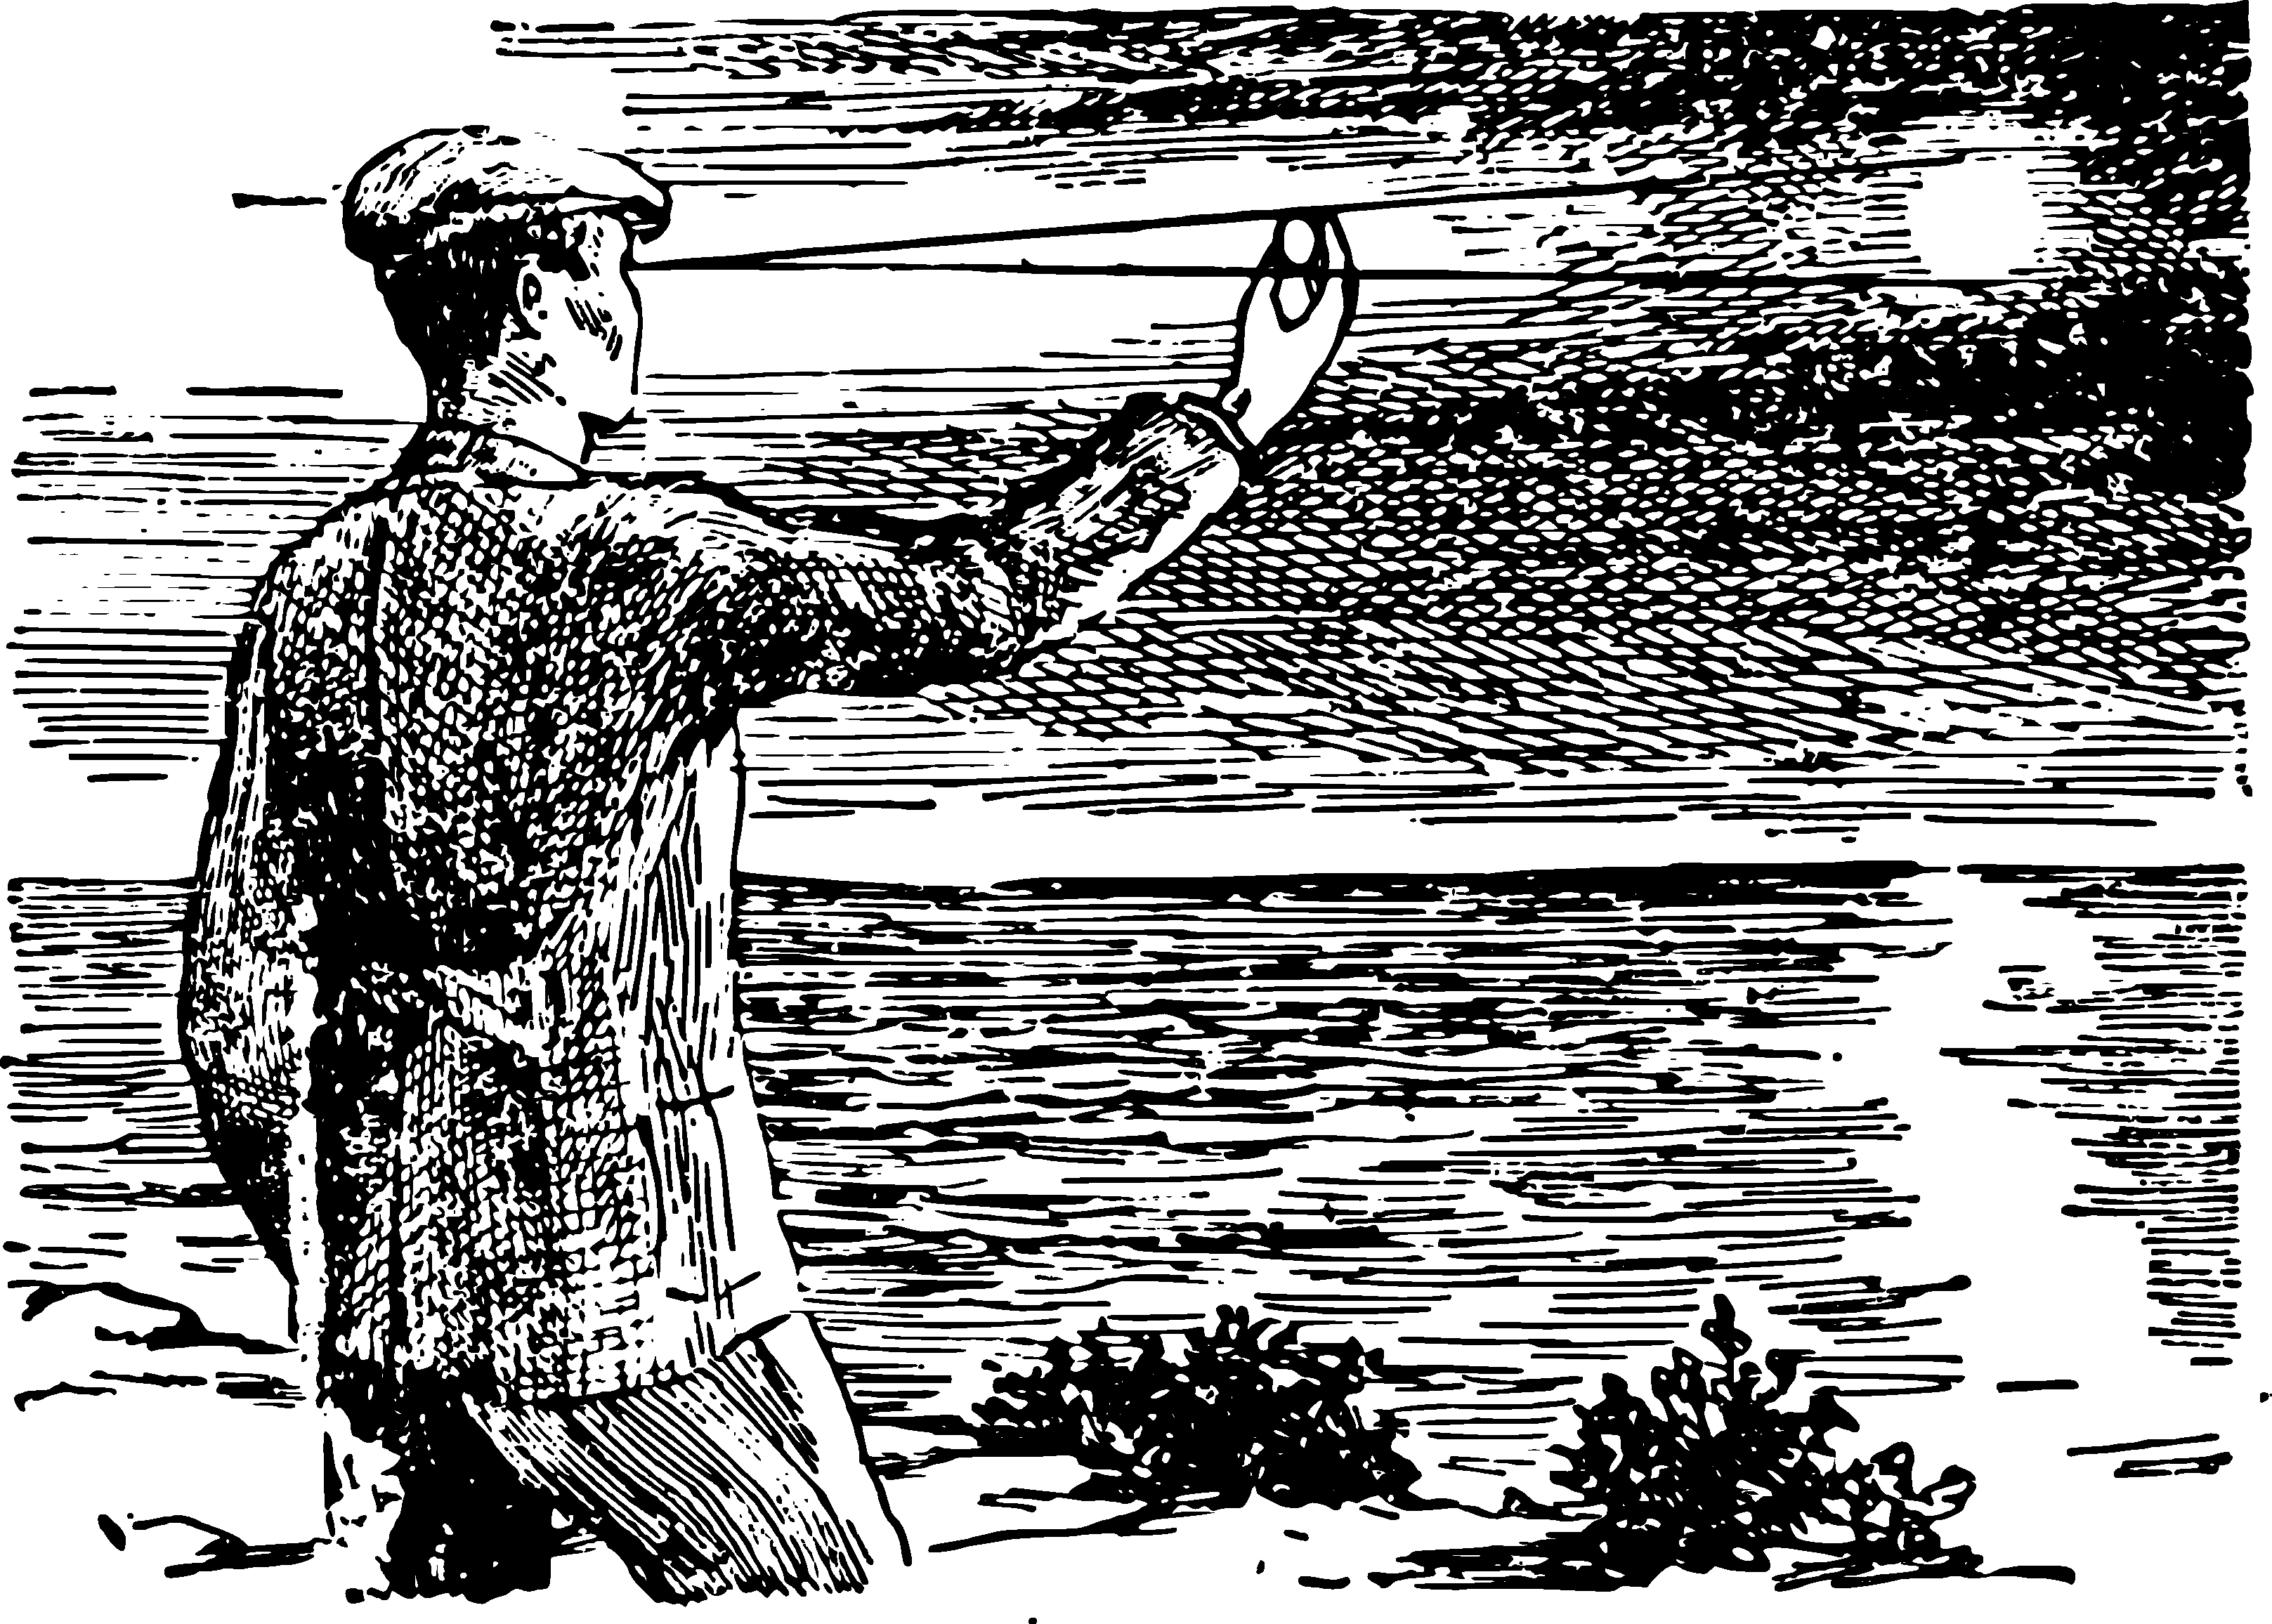
\includegraphics[width=0.9\textwidth]{figures/ch-03/fig-061.pdf}
\sidecaption{What is the angle of view or angular size of the object.\label{fig-061}}
\end{figure}

And when the apparent size of the Moon in the sky is assessed by comparing it with the sizes of a plate, an apple, and so forth, such answers are either completely meaningless or should imply that the Moon is visible in the sky at the same angle as the plate or apple. But such an indication alone is still insufficient: after all, we see a plate or an apple under different angles depending on their distance: up close -- under larger angles, far away -- under smaller ones. To introduce clarity, it is necessary to specify from what distance the plate or apple is being observed. Comparing the sizes of distant objects with the sizes of others, the distance of which is not indicated, is a very common literary technique employed by even first-rate writers. It creates a certain impression due to its closeness to the familiar psychology of most people, but it does not produce a clear image\ldots{} Here's an example from Shakespeare's \emph{King Lear}; it describes (by Edgar) the view from a high cliff by the sea:
\begin{quote}
\emph{How terrifying! How my head spins!\\
How low to cast my gaze\ldots{}\\
The rooks and crows that flutter there in the air at mid-distance,\\ Seem barely as large as flies. Halfway down Hangs a man gathering seaweed\dots{} \\
What a dreadful trade! He seems to me no bigger than his head.\\
The fishermen walking along the shore -- like mice;\\
and that tall ship at anchor has shrunk to the size of its boat;\\ its boat -- a floating dot, As if too small for sight\dots{}}
\end{quote}
These comparisons would provide a clear idea of distance if accompanied by indications of the degree of remoteness of the objects being compared (mice, the human head, crows, boat \dots{}). Similarly, when comparing the size of the moon with that of a plate or apples, indications of how far these everyday objects should be from the eye are necessary.

This distance turns out to be much greater than commonly thought. Holding an apple at arm's length, you not only obscure the Moon but also a significant portion of the sky. Suspend the apple on a string and gradually move away from it until it just covers the full lunar disk: in this position, the apple and the Moon will have the same apparent size for you. By measuring the distance from your eye to the apple, you will find that it is approximately 10 meters. This is how far you would need to move the apple away from you for it to truly seem to be the same size as the Moon in the sky! A plate, on the other hand, would need to be moved about 80 meters away from you, or about fifty steps.

What is said may seem unbelievable to anyone hearing it for the first time; however, it is indisputable and follows from the fact that we perceive the Moon at an angle of only \emph{half a degree}. We rarely have to estimate angles in our everyday lives, and therefore most people have a very vague idea of the magnitude of an angle with a small number of degrees, such as an angle of \ang{1}, \ang{29}, or \ang{59} (not to mention surveyors, draftsmen, and other specialists accustomed to practically measuring angles). We only estimate large angles more or less reasonably, especially if we manage to compare them with angles familiar to us between the hands of a clock; everyone, of course, is familiar with angles of \ang{90}, \ang{60}, \ang{30}, \ang{120}, \ang{150}, which we are so accustomed to seeing on a dial (at 8 o'clock, 2 o'clock, 1 o'clock, 4 o'clock, 5 o'clock) that even without distinguishing the numbers, we guess the time based on the size of the angle between the hands. But we usually see small and individual objects at much smaller angles and therefore completely lack the ability to even approximately estimate angles of view.


\section{Angle of View}
\label{sec-3.2}

To provide a concrete example of a one-degree angle, let's calculate how far an average-height person (1.7 meters) should move away from us to appear at such an angle. Translating the problem into the language of geometry, let's say we need to calculate the radius of a circle, the arc of which at \ang{1} has a length of 1.7 meters (strictly speaking, not an arc, but a chord, but for small angles, the difference between the lengths of the arc and the chord is negligible). We reason as follows: if the arc at \ang{1} equals 1.7 meters, then the full circumference containing \ang{360} will have a length of $1.7 \times 360 = \SI{610}{\meter}$, and the radius will be $1/2\pi$ the length of the circumference; if we take the value of $\pi$ as approximately 22/7, then the radius will be equal to
\begin{equation*}%
 \frac{610}{44/7} \approx \SI{98}{\meter}.
\end{equation*}
\begin{figure}[h!]
\centering
\includegraphics[width=0.9\textwidth]{figures/ch-03/fig-062.pdf}
\sidecaption{The human figure is visible from a distance of about hundred meters at an angle of \ang{1}.\label{fig-062}}
\end{figure}
So, a person appears at an angle of \ang{1} if they are approximately at a distance of 100 meters from us (\figr{fig-062}). If they move twice as far away -- to 200 meters -- they will be seen at an angle of half a degree; if they approach to a distance of 50 meters, the angle of view will increase to \ang{2}, and so on. It is also easy to calculate that a stick of 1 meter in length should appear to us at an angle of 1° at a distance of $360/(44/7) = \SI{57}{\meter}$.

At the same angle, we perceive an object of 1 cm from a distance of 57 cm, 1 km from a distance of 57 km, and so on -- in general, any object from a distance 57 times greater than its diameter. If we remember this number -- 57, we can quickly and easily perform all calculations related to the angular size of an object. For example, if we want to determine how far we need to move an apple with a diameter of 9 cm to see it at an angle of \ang{1}, it is sufficient to multiply 9 by 57 -- we get 513 cm, or about 5 meters; from twice the distance, it is perceived at half the angle -- half a degree, i.e., it appears the size of the Moon.

In the same way, for any object, we can calculate the distance at which it appears to be the same size as the lunar disk.

\section{Plate and Moon} 
\label{sec-3.3}

\ques At what distance should a plate with a diameter of 25 cm be moved away to appear the same size as the Moon in the sky?

\ans $\SI{25}{\centi\meter} \times 57 \times 2 = \SI{2850}{\centi\meter} = \SI{28}{\meter}$.

\section{Moon and Copper Coins} 
\label{sec-3.4}

\ques Perform the same calculation for a five-kopeck coin (diameter 25 mm) and a three-kopeck coin (22 mm).

\ans For the five-kopeck coin: \(0.025 \text{ m} \times 57 \times 2 = 2.85 \text{ meters}\),
For the three-kopeck coin: \(0.022 \text{ m} \times 57 \times 2 = 2.514 \text{ meters}\).

If it seems unbelievable to you that the Moon appears no larger than a two-kopeck coin from a distance of four steps or an ordinary pencil from a distance of 80 cm, -- hold the pencil at arm's length against the full Moon disk: it will easily cover it. Strangely enough, the most suitable comparison object for the Moon in terms of perceived size is not a plate, not an apple, not even a cherry, but a pea or, even better, a match head! Comparing it to a plate or an apple implies moving them to an unusually large distance; we see an apple in our hands or a plate on the dining table ten to twenty times larger than the lunar disk. And only a match head, which we examine at a distance of 25 cm from the eye (`distance of distinct vision'), is seen at an angle of half a degree, i.e., the same size as the Moon.

The fact that the lunar disk deceptively appears to grow in the eyes of most people by 10 to 20 times is one of the most curious optical illusions. It depends, one might think, mostly on the \emph{brightness} of the Moon: the full moon stands out against the sky much more sharply than plates, apples, coins, and other comparison objects do amidst the surrounding environment.\sidenote{For the same reason, the incandescent filament of an electric light bulb seems to us much thicker than in a cold, non-luminous state.}

This illusion is imposed on us with such irresistible force that even artists, distinguished by a keen eye, succumb to it alongside others and depict the full moon in their paintings much larger than it should be. It is enough to compare the landscape painted by an artist with a photograph to be convinced of this.

The same applies to the Sun, which we see from Earth at the same angle of half a degree; although the true diameter of the solar sphere is 400 times larger than that of the lunar one, its distance from us is also 400 times greater.


\section{Sensational Photographs}
\label{sec-3.5}

To explain the important concept of the angle of view, let's deviate a bit from our main topic — geometry in open fields — and provide a few examples from the realm of photography.

On the movie screen, you've surely seen such catastrophes as train collisions or such incredible scenes as a car driving on water.

Recall the movie `Captain Grant's Children.' What a strong impression -- isn't it? -- the scenes of the shipwreck during the storm or the sight of crocodiles surrounding the boy stuck in the swamp left on you. Of course, no one thinks that such photographs were taken directly from real life. But how were they obtained?
\begin{figure}[h!]
\centering
\includegraphics[width=0.9\textwidth]{figures/ch-03/fig-063.pdf}
\sidecaption{Preparing a train accident for filming.\label{fig-063}}
\end{figure}


The secret is revealed by the illustrations attached here. In \figr{fig-063}, you see the `catastrophe' of a toy train in a toy setting; in \figr{fig-064} -- a toy car being pulled on a string behind an aquarium. This is the `nature' from which the film was shot. But why do we succumb to the illusion when we see these images on the screen, as if we were looking at real trains and cars? After all, here, in the illustrations, we would immediately notice their miniature size, even if we couldn't compare them with the size of other objects. The reason is simple: toy trains and cars are filmed for the screen from a very close distance; therefore, they appear to the viewer at approximately the same angle of view as we usually see real trains and cars. That's the whole secret of the illusion.

\begin{figure}[h!]
\centering
\includegraphics[width=0.9\textwidth]{figures/ch-03/fig-064.pdf}
\sidecaption{The underwater road trip.\label{fig-064}}
\end{figure}

Or here's another frame from the movie `Ruslan and Ludmila' (\figr{fig-065}). A huge head and a small Ruslan on a horse. The head is placed on a model field close to the camera. And Ruslan on the horse -- at a considerable distance. That's the entire secret of the illusion.

\begin{figure}[h!]
\centering
\includegraphics[width=0.9\textwidth]{figures/ch-03/fig-065.pdf}
\sidecaption{A shot from the movie \emph{Ruslan and Lyudmila}.\label{fig-065}}
\end{figure}

\section{Reservoir Set Decoration}
\label{sec-3.6}

\figr{fig-066} is another example of an illusion based on the same principle. You see a strange landscape reminiscent of the nature of ancient geological epochs: bizarre trees resembling giant mosses, on them -- huge water drops, and in the foreground -- a gigantic monster resembling harmless frogs. Despite such an unusual view, the drawing is made with subtlety: it's nothing but a small patch of soil in the forest, only drawn from an unusual angle of view. We never see moss stems, water drops, frogs, etc., at such a large angle of view, and therefore the drawing seems so alien, unfamiliar to us. Before us is a landscape as we would see it if we were shrunk to the size of an ant. 

\begin{marginfigure}[-1cm]%[h!]
\centering
\includegraphics[width=\textwidth]{figures/ch-03/fig-066.pdf}
\sidecaption{Mysterious landscape depicted from nature.\label{fig-066}}
\end{marginfigure}

Swindlers from bourgeois newspapers act in the same way to create fake reportage photographs. One foreign newspaper once published a note criticising the city administration for allowing huge snow mountains to form on the city streets. To support this, an impressive photo of one such mountain was provided (\figr{fig-067}, left). Upon examination, it turned out that the nature for the photograph was a small snowdrift, taken by the `joker' photographer from a very close distance, i.e., at an unusually large angle of view (\figr{fig-067}, right). 

\begin{figure}[h!]
\centering
\includegraphics[width=\textwidth]{figures/ch-03/fig-067.pdf}
\sidecaption{Snow mountain in a photograph (left) and in nature (right).\label{fig-067}}
\end{figure}

Another time, the same newspaper reproduced a photo of a wide crevice in the rock near the city; it served, according to the newspaper, as the entrance to an extensive underground cave, where a group of careless tourists who dared to enter the cave for exploration disappeared without a trace. A volunteer search party equipped to search for the lost discovered that the crevice was photographed\dots{} from a barely noticeable crack in the icy wall, a centimetre wide!



\section{Living Protractor}
\label{sec-3.7}

Making a simple protractor device yourself is not very difficult, especially if you use a protractor. But sometimes even a homemade protractor may not be at hand during a countryside walk. In such cases, you can rely on the services of a ``living protractor'' that is always with us. These are our own fingers. To use them for a rough estimate of viewing angles, you just need to make a few preliminary measurements and calculations.

First of all, you need to determine at what angle we see the fingernail of our outstretched index finger. The usual width of a nail is \SI{1}{\centi\meter}, and its distance from the eye in such a position is about \SI{60}{\centi\meter}; therefore, we see it at an angle of about \ang{1} (slightly less because an angle of \ang{1} would be at a distance of \SI{57}{\centi\meter}). For teenagers, the nail is smaller, but the arm is shorter, so the viewing angle for them is approximately the same -- \ang{15}. The reader would do well to perform this measurement and calculation for themselves, relying on book data, to make sure the result is not too far from \ang{15}; if the deviation is significant, you should try another finger.

Knowing this, you have a way to estimate small viewing angles literally with your bare hands. Each distant object, which is just covered by the fingernail of your outstretched index finger, is seen by you at an angle of \ang{1} and, therefore, is 57 times farther away than its width. If the nail covers half of the object, it means its angular size is \ang{2}, and the distance is equal to 28 widths.

The Full Moon covers only half of the nail, i.e., it is seen at an angle of half a degree, meaning it is 114 times its width away from us; here is a valuable astronomical measurement made literally with bare hands!

For larger angles, use the knuckle of your thumb, holding it bent on your outstretched hand. For an adult, the length (note: length, not width) of this joint is about 3.5 cm, and the distance from the eye with an outstretched arm is about 55 cm. It is easy to calculate that the angular size in this position should be about \ang{4}. This provides a means to estimate angles of \ang{4} (and therefore \ang{8}).

Here, you should also add two more angles that can be measured with your fingers -- namely, those under which the intervals between fingers are seen when your middle and index fingers are spread as wide as possible; and between your thumb and index finger, also spread to the maximum. It is easy to calculate that the first angle is approximately \ang{7}-\ang{8}, and the second is \ang{15}-\ang{16}.

There can be many cases to apply your living protractor during walks in open spaces. Suppose a freight car is visible in the distance, which is covered by approximately half of the knuckle of your outstretched thumb, i.e., it is visible at an angle of about \ang{2}. Since the length of a freight car is known (about \SI{6}{\meter}), you can easily find out how far you are from it: $6 \times 28 \approx \SI{170}{\meter}$ or so. A method that does not seem to promise good results, but after a short exercise you will learn to appreciate the services of this ``living ecker''\sidenote{An ``ekker'' is a surveying instrument for drawing lines on the ground at right angles.}, the measurement is, of course, rough, but still more reliable than an ungrounded estimate just by sight.

\begin{figure}[h!]
\centering
\includegraphics[width=0.8\textwidth]{figures/ch-03/fig-068.pdf}
\sidecaption{Mapping of the lake on the plan.\label{fig-068}}
\end{figure}

Additionally, using your living protractor, you can, in the absence of any tools, measure the angular height of luminaries above the horizon, the mutual separation of stars in degrees, the apparent sizes of a meteor's trail, etc. Finally, knowing how to make right angles on the ground without instruments, you can draw up a plan of a small area using the method whose essence is clear from the illustration, for example, when surveying a lake (\figr{fig-068}), measure rectangle $ABCD$, as well as the lengths of the perpendiculars dropped from prominent points on the shore, and the distances from their bases to the vertices of rectangle $ABCD$. In short, being in Robinson Crusoe's situation, knowing how to use your own hands to measure angles (and your feet to measure distances) could be useful for a variety of needs.

\section{Jacob's Staff}
\label{sec-3.8}

If you wish to have more accurate angle measures than the simple ``living protractor'' described earlier, you can make yourself a simple and convenient device that was once used by our ancestors. This is called ``Jacob's staff'' after its inventor -- a device that was widely used by sailors until the 18th century (\figr{fig-069}), before it was gradually replaced by even more convenient and precise instruments (sextants).

\begin{figure}[h!]
\centering
\includegraphics[width=\textwidth]{figures/ch-03/fig-069.pdf}
\sidecaption{Jacob's staff and a diagram of its use.\label{fig-069}}
\end{figure}

It consists of a long ruler $AB$, about 170–100 cm, along which a perpendicular block $CD$ can slide; both parts $CO$ and $OD$ of the sliding block are equal to each other. If you want to determine the angular distance between the stars $S$ and $S'$ using this block (\figr{fig-069}), you attach the end $A$ of the ruler to your eye (where a perforated plate is attached for convenience of observation) and direct the ruler so that the star $S'$ is visible at the end $B$ of the ruler; then you move the crosspiece $CO$ along the ruler until the star $S$ is just visible at the end $C$ (\figr{fig-069}). Now all that remains is to measure the distance $AO$ in order to calculate the value of the angle $SAS'$ using the length of the $CO$. Those familiar with trigonometry will understand that the tangent of the desired angle is equal to the ratio of $CO/AO$. Our ``field trigonometry'', presented in the fifth chapter, is also sufficient for performing this calculation: you calculate the length $AC$ using the Pythagorean theorem, then find angle $C$, whose sine is equal to $CO/AC$.

Finally, you can find the desired angle graphically; by drawing triangle $ACO$ on paper to scale, you measure angle $A$ with a protractor, or if you don't have one, by the method described in our ``field trigonometry'' (see Chapter~\ref{ch-05}).

\begin{figure}[h!]
\centering
\includegraphics[width=0.9\textwidth]{figures/ch-03/fig-070.pdf}
\sidecaption{Determination of the angular distance between stars using Jacob's staff.\label{fig-070}}
\end{figure}

What is the other half of the crosspiece for? In case the angle to be measured is too large to be measured by the method described above. In that case, instead of directing the ruler $AB$ toward the star $S'$, you aim segment $AD$ toward the point $S'$, moving the crosspiece so that its end $C$ coincides with the star $S$ at the same time (\figr{fig-070}). Finding the angle $SAS'$ by calculation or construction is, of course, not difficult.

To avoid having to make calculations or constructions each time you measure, you can perform them in advance, even when making the device, and mark the results on the ruler $AB$; then, when aiming the device at the stars, you only need to read the reading recorded at point $O$ — this is the value of the measured angle.


\begin{center}
\includegraphics[width=0.3\textwidth]{figures/ch-03/fig-ch-03-tail.pdf}
\end{center}



















% !TEX root = perelman-geometry.tex
%!TEX TS-program = pdflatex
%!TEX encoding = UTF-8 Unicode

\setchapterpreamble[o]{\includegraphics[width=1.2\textwidth]{figures/ch-04/fig-ch-04-head.pdf}\bigskip}

\chapter{Geometry on the Road}
\label{ch-04}

\section{The Art of Measuring by Steps}
\label{sec-4.1}


While out for a countryside walk along a railway track or on a highway, you can perform a series of interesting geometric exercises.

First, use the highway to measure the length of your step and walking speed. This will allow you to -- measure distances by steps -- an art that is acquired quite easily after a short practise. The main thing here is to get used to making steps of the same length every time, i.e., to adopt a certain `measured' gait.

On the highway, every 100 meters, there is a white stone; by walking such a 100-meter interval with your usual `measured' step and counting the number of steps, you can easily find the average length of your step. Such measurement should be repeated annually, for example, every spring, because the length of a step, especially in young people, does not remain constant.

It is worth noting an interesting relationship discovered by repeated measurements: the average length of an adult's step is approximately half of their height, measured to eye level. For example, if a person's height to their eyes is 1 meter 40 centimetres, then the length of their step is about 70 centimetres. It's interesting to verify this rule whenever possible.

In addition to knowing the length of your stride, it's also useful to know your walking speed -- the number of kilometres you cover per hour. Sometimes the following rule is used for this: we walk as many kilometeres per hour as we take steps in three seconds; for example, if we take four steps in three seconds, then we walk 4 km per hour. However, this rule is only applicable when the length of the stride is known. It's not difficult to determine it: denoting the length of the stride in meters as $x$, and the number of steps in three seconds as $p$, we have the equation
\begin{equation*}%
\frac{3600}{3} \cdot nx = n \cdot 1000, 
\end{equation*}
from which $1200x = 1000$ and $x = 1000/1200 \si{\meter}$, i.e., about 80—85 cm. This is a relatively large stride; people of tall stature make such strides. If your stride differs from 80—85 cm, then you will need to measure your walking speed in a different way, by determining the time it takes you to cover the distance between two roadside posts using a clock.

\section{Eye-meter}
\label{sec-4.2}

It's pleasant and useful not only to measure distances without a measuring tape, but also to estimate them directly by eye without measurement. This skill is achieved only through practice. In my school years, when I participated in summer excursions out of town with a group of friends, such exercises were very common for us. They were carried out in the form of a special sport, invented by ourselves -- in the form of a competition for the accuracy of the eye-meter. When we went out on the road, we would visually mark some roadside tree or other distant object, and the competition would begin.

``How many steps to the tree?'' someone from the participants would ask.

The rest would give their estimated number of steps, and then together count the steps to determine whose estimate was closer to the truth -- that person would be the winner. Then it was their turn to mark an object for the eye-meter distance estimation.

Whoever determined the distance more accurately than the others would receive one point. After 10 times, the points were counted: the one with the most points was considered the winner of the competition.

I remember that at first our distance estimates were given with rough errors. But very soon, much faster than expected, we sharpened our skills in the art of estimating distances by eye, making very few mistakes. Only with a sharp change in surroundings, for example, when transitioning from an open field to sparse forest or to a bush-covered clearing, when returning to dusty, narrow city streets, or at night, with the deceptive illumination of the moon, would we catch each other making significant errors. However, we soon learned to adapt to all circumstances, mentally taking them into account during eye-meter estimates. Finally, our group reached such perfection in eye-meter distance estimation that we had to completely abandon this sport: everyone guessed equally well, and the competitions lost their interest. But we acquired a decent eye-meter, which served us well during our wanderings in the countryside.

It's curious that eye-metering seems to be independent of visual acuity. Among our group was a nearsighted boy who not only didn't lag behind the others in the accuracy of eye-meter distance estimation but sometimes even emerged as the winner of the competitions. Conversely, a boy with perfectly normal vision couldn't master the art of determining distances by eye at all. Later, I had to observe the same phenomenon when estimating the height of trees using the eye-meter method: practising this with students -- not for play anymore, but for the needs of future professions -- I noticed that nearsighted individuals mastered this skill just as well as others. This can be a consolation for the nearsighted: without having perfect vision, they are still capable of developing quite satisfactory eye-metering skills.

Practising eye-metering distance estimation can be done at any time of the year, in any setting. Walking along the city streets, you can set yourself eye-metering tasks, trying to guess how many steps to the nearest lamp-post or to various objects along the way. In bad weather, you can effectively fill the time with such activities while traversing empty streets.

The military pay a lot of attention to eye-metering distance estimation: a good eye-meter is necessary for a scout, a marksman, an artilleryman. It's interesting to learn about the signs they use in the practise of eye-metering estimations. Here are a few notes from the artillery textbook:

``On-eye distances are determined either by the skill of distinguishing visible objects at different distances from the observer to a certain degree of clarity, or by estimating distances using some familiar visual stretch of 100–200 steps, which seems smaller the further away it is from the observer.''

``When determining distances based on the clarity of visible objects, it should be noted that objects illuminated or brighter in colour appear closer in terrain or on water; objects positioned higher than others; groups compared to individual objects and generally larger objects.''

\begin{figure}[h!]
\centering
\includegraphics[width=0.8\textwidth]{figures/ch-04/fig-079.pdf}
\sidecaption{The tree behind the hillock seems close.\label{fig-079}}
\end{figure}

``You can follow the following signs: up to 50 steps, you can clearly distinguish people's eyes and mouth; at 100 steps, eyes appear as dots; at 200 steps, buttons and uniform details can still be distinguished; at 300 steps, the face is visible; at 400 steps, leg movements can be discerned; at 500 steps, the colour of the uniform is visible.''

At the same time, the most experienced eye may make an error of up to 10\% in either direction of the determined distance.


\begin{figure}[h!]
\centering
\includegraphics[width=0.8\textwidth]{figures/ch-04/fig-080.pdf}
\sidecaption{Climb up the hill, and the tree is still the same distance away.\label{fig-080}}
\end{figure}

There are cases, however, when eye-metering errors are much more significant. Firstly, when determining distance on a uniform, completely one-coloured surface -- on the smooth surface of a river or lake, on a clean sandy plain, on a densely overgrown field. Here, the distance always seems smaller than the true one; estimating it by eye, we make an error of two-fold, if not more. Secondly, errors are easily possible when determining the distance to an object whose base is obscured by a railway embankment, a small hill, a building, or any other elevation. In such cases, we involuntarily consider the object to be not behind the elevation, but on it itself, and therefore make an error again in the direction of reducing the determined distance (\figr{fig-079} and \figr{fig-080}).

In such cases, relying on the eye-meter is dangerous, and resorting to other methods of distance estimation, which we have already discussed and will continue to discuss, becomes necessary.


\section{Slopes}
\label{sec-4.3}

Alongside the railway track, besides the mile (more precisely -- kilometre) posts, you also see other low poles with inscriptions on small boards, like those shown in \figr{fig-081}.

\begin{figure}[h!]
\centering
\includegraphics[width=\textwidth]{figures/ch-04/fig-081.pdf}
\sidecaption{``Slope Signs.''\label{fig-081}}
\end{figure}


These are `slope signs.' In the first one, for example, the upper number 0.002 means that the gradient of the track here (in which direction -- indicated by the position of the board) is equal to 0.002: the track rises or descends by 2 mm for every thousand millimetres. And the lower number 140 indicates that such a gradient extends for 140 m, where another sign is placed with a notation of a new gradient. (When roads were not yet reorganised according to the metric system, such a board indicated that over a distance of 140 fathoms, the track rises or descends every fathom by 0.002 fathoms.) The second board with the inscription 0.006/55 indicates that over the next 55 m, the track rises or descends by 6 mm for every meter.

Knowing the meaning of the slope signs, you can easily calculate the difference in height between two adjacent points on the track marked by these signs. In the first case, for example, the height difference is $0.002 \times 140 = \SI{0.28}{\meter}$; in the second case -- $0.006 \times 55 = \SI{0.33}{\meter}$.

In railway practise, as you can see, the magnitude of the track gradient is not determined in degrees. However, it is easy to convert these track gradient markings into degrees. If $AB$ (\figr{fig-081}) is the path line, $BC$ is the height difference between points $A$ and $B$, then the inclination of the path line $AB$ to the horizontal line $AC$ will be marked on the post by the ratio $BC/AC$. Since angle $A$ is very small, we can take $AB$ and $AC$ as radii of a circle, the arc of which is $BC$.\sidenote[][-5cm]{To another reader, it may seem perhaps unacceptable to consider the inclined $AB$ equal to the perpendicular $AC$; Therefore, it is instructive to ensure how small the difference in length between $AC$ and $AB$ is when $BC$ is, for example, $0.01$ of $AB$. By the Pythagorean theorem, we have:
\begin{align*}%
AC^{2} & = \sqrt{AB^{2} - \frac{AB^{2}}{100}}\\
& = \sqrt{0.9999\, AB^{2}} \approx 0.99995 \, AB^{2}.
\end{align*}
The difference in length is only $0.00005$. For approximate calculations, such a small error can certainly be neglected.
} Then the calculation of angle $A$, if the ratio $BC:AB$ is known, will not be difficult. With a slope, for example, marked as 0.002, we reason as follows: with an arc length equal to 1/57 radius, the angle is \ang{1} (see page~\pageref{fig-062}); what angle corresponds to an arc of 0.002 radii? We find its value $x$ from the proportion 
\begin{align*}%
\frac{x}{\ang{1}} & = \frac{0.002}{1/57},\,\, \text{from where,}\\
x & = 0.002 \times 57 = \ang{0.11},
\end{align*}
i.e., about \ang{;7}.
 
Only very small gradients are allowed on railway tracks. We have set the maximum gradient at 0.008, i.e., in degrees, $0.008 \times 57$ -- less than \ang{0.5}: this is the maximum gradient. Only for the Transcaucasian Railway, gradients up to 0.025 are allowed as an exception, which corresponds to almost \ang{1.5} in degrees.

Such insignificant gradients are completely unnoticed by us. A pedestrian begins to feel the slope under their feet only when it exceeds $\nicefrac{57}{24}$: this corresponds to approximately \ang{2.5} in degrees.

Having walked along the railway track for several kilometres and noted the observed gradient signs, you can calculate how much you have ascended or descended in total, i.e., what is the difference in height between the starting and ending points.


\ques You started a walk along the railway track at a post marked with an ascent of 0.004/153 miles and encountered the following signs further along\sidenote{Sign 0.000 means a horizontal section of the path (``platform'').}: 
\begin{small}
\begin{center}
\begin{tabular}{ccccc}
\toprule
Platform & Ascent & Ascent & Platform & Descent\\
\midrule 
$\dfrac{0.000}{60}$ & $\dfrac{0.0017}{84}$ & $\dfrac{0.0032}{121}$ & $\dfrac{0.000}{45}$ & $\dfrac{0.004}{210}$ \\
\bottomrule
\end{tabular}
\end{center}
\end{small}
You finished the walk at another slope sign. What distance did you travel, and what is the difference in height between the first and last signs?

\ans Total distance travelled: 
\begin{equation*}%
153 + 60 + 84 + 121+ 45 + 210 = \SI{673}{\meter}.
\end{equation*}
You went up by
\begin{equation*}%
0.004 \times 153 + 0.0017 \times 84 + 0.0032 \times 121 = \SI{1.15}{\meter},
\end{equation*}
and descended:
\begin{equation*}%
0.004 \times 210 = \SI{0.84}{\meter}.
\end{equation*}
Therefore, in total, you ended up higher than the starting point by $1.15 - 0.84 = \SI{0.31}{\meter}$.

\section{Heap of Gravel}
\label{sec-4.4}

Heap of gravel at the edges of the road also presents an object worthy of attention for the ``geometer in the open air.'' By asking what volume the heap in front of you contains, you set yourself a geometric problem, quite intricate for someone accustomed to overcoming mathematical difficulties only on paper or on the blackboard. 

\begin{figure}[h!]
\centering
\includegraphics[width=0.9\textwidth]{figures/ch-04/fig-082.pdf}
\sidecaption{For the problem of the gravel heap.\label{fig-082}}
\end{figure}

You have to calculate the volume of a cone, the height and radius of which are not directly measurable. However, nothing prevents you from determining their value indirectly. You will find the radius by measuring the circumference of the base with a ruler or string and dividing it by $2\pi$.\sidenote{In practice, this action is replaced by multiplication by the reciprocal, if looking for the diameter, and by 0.159 if calculating the radius.} 

The height poses a greater challenge (\figr{fig-082}): you have to measure the length of the generatrix $AB$ or, as the road surveyors do, both generatrices $ABC$ at once (by laying the measuring tape over the apex of the heap), and then, knowing the radius of the base, calculate the height $BD$ using the Pythagorean theorem. Let's consider an example.

\ques The circumference of the base of a conical heap of gravel is 12.1 m; the length of the two generatrices is 4.6 m. What is the volume of the heap?

\ans The radius of the base of the heap is 
\begin{equation*}%
12.1 \times 0.159 \,\, \text{(instead of 12.1/6.28)} = \SI{1.9}{\meter}.
\end{equation*}
The height is 
\begin{equation*}%
\sqrt(2.3^{2} - 1.9^{2}) =  \SI{1.2}{\meter},
\end{equation*}
hence the volume of the heap is 
\begin{equation*}%
\frac{1}{3} \times 3.14 \times 1.9^{2} \times 1.2 =  \SI{4.6}{\meter\cubed}
\end{equation*}
(approximately 1/2 cubic fathoms in previous measurements).

Typically, the standard volume measurements for gravel heaps on our roads were $\nicefrac{1}{2}$, $\nicefrac{1}{4}$, and $\nicefrac{1}{8}$ cubic fathoms, i.e., in metric units, 4.8, 2.4, and 1.2 cubic meters.
\clearpage


\section{The Proud Hill}
\label{sec-4.5}

Looking at conical heaps of gravel or sand brings to mind an ancient legend of Eastern peoples, retold by Pushkin in \emph{The Miserly Knight}:

\begin{quote}
\emph{I read somewhere,\\
That once a king ordered his warriors\\
To carry earth by handfuls into a heap, --\\
And a proud hill rose up,\\
And the king could from the heights with joy survey\\
Both the valley, covered with white tents,\\
And the sea, where ships sailed.}
\end{quote}

This is one of those few legends in which, despite its seeming plausibility, there is not a grain of truth. It can be proven by geometric calculation that if some ancient despot had decided to undertake such an endeavour, he would have been discouraged by the meagerness of the result: before him would have risen such a pitiful pile of earth that no imagination could inflate it into the legendary ``proud hill''.

Let's make an approximate calculation. (How many warriors could an ancient king have? Ancient armies were not as numerous as they are today. An army of 100,000 people was already very impressive in size. Let's stick with this number, i.e., assume that the hill was composed of 100,000 handfuls. Grab the largest handful of earth and fill a glass with it: you won't fill it with just one handful. Let's assume that the handful of an ancient warrior equalled in volume $\nicefrac{1}{5}$ (\si{\deca\meter\cubed}). Hence, the volume of the hill is:
\begin{equation*}%
\frac{1}{5} \times 100000 = 20,000\, \si{\deca\meter\cubed} = 20 \si{\meter\cubed}.
\end{equation*}
Thus, the hill represented a cone with a volume of no more than 20 cubic meters. Such a modest volume is already disappointing. But let's continue the calculations to determine the height of the hill. To do this, we need to know the angle formed by the generatrices of the cone with its base. In our case, we can assume it to be equal to the angle of natural slope, i.e., \ang{45}: steeper slopes cannot be allowed as the earth would collapse (it would be more plausible to take an even shallower slope, for example, one and a half). Stopping at an angle of \ang{45}, we conclude that the height of such a cone is equal to the radius of its base; therefore,
\begin{align*}%
20 & = \frac{\pi x^{3}}{3}, \,\, \text{hence,}\\
x & = \sqrt[3]{\frac{60}{\pi}} =  2.4 \si{\meter}.
\end{align*}
One must possess a rich imagination to call a pile of earth 2.4 meters (1.5 human height) a ``proud hill.'' By making the calculation for the case of a one and a half slope, we would have obtained an even more modest result.

Attila had the most numerous army known in the ancient world. Historians estimate it to be 700,000 people. If all these warriors participated in building the hill, a heap taller than the one we calculated would have been formed, but not significantly: since the volume would be seven times larger than ours, the height would exceed the height of our heap by only 1.7 times; it would be equal to $2.4 \times 1.9 = 4.6$ meters. It is doubtful that a mound of such dimensions could satisfy the ambition of Attila.

From such small elevations, it was easy, of course, to see ``the valley covered with white tents''," but surveying the sea was possible only if the affair took place not far from the shore.

We will discuss how far one can see from a certain height in the sixth chapter.


\section{At a Road Curve}
\label{sec-4.6}

Neither highways nor railways ever make sharp turns; they always transition smoothly from one direction to another, without breaks, in an arc. This arc is usually part of a circle arranged so that the straight sections of the road serve as tangents to it. 

\begin{figure}[h!]
\centering
\includegraphics[width=0.9\textwidth]{figures/ch-04/fig-083.pdf}
\sidecaption{Road rounding.\label{fig-083}}
\end{figure}

For example, in \figr{fig-083}, the straight sections $AB$ and $CD$ of the road are connected by the arc $BC$ so that $AB$ and $CD$ touch (geometrically) this arc at points $B$ and $C$, i.e., $AB$ forms a right angle with radius $OB$, and $CD$ forms the same angle with radius $OC$. This is done, of course, to smoothly transition the path from a straight direction to a curved part and back again.

The radius of a road curve is usually taken to be quite large -- on railways, not less than 600 meters; the most common radius of curvature on the main railway track is 1000 or even 2000 m.



\section{Radius of Curvature}
\label{sec-4.7}


Standing near one of such curves, could you determine the magnitude of its radius? This is not as easy as finding the radius of an arc drawn on paper. On a drawing, it's simple: you draw two arbitrary chords and draw perpendiculars from their midpoints: the point of their intersection is known to be the centre of the arc; the distance from it to any point on the curve is the desired length of the radius.

But to make a similar construction on the ground would, of course, be very inconvenient: after all, the centre of the curve is 1-2 meters from the road, often in an inaccessible place. It would be possible to make the construction on a plan, but taking the curves off onto a plan is also not an easy task.

\begin{marginfigure}[-4cm]%[h!]
\centering
\includegraphics[width=\textwidth]{figures/ch-04/fig-084.pdf}
\sidecaption{To calculate the radius of curvature.\label{fig-084}}
\end{marginfigure}

All these difficulties are eliminated if one resorts not to constructing, but to calculating the radius. For this purpose, the following method can be used. We mentally supplement the arc $AB$ of the curve (\figr{fig-084}) to a circle. Connecting arbitrary points $C$ and $D$ of the arc of the curve, we measure the chord $CD$, as well as the ``arrow'' $EF$ (i.e., the height of the segment CED). From these two data, it is already not difficult to calculate the desired length of the radius.

Considering the lines $CD$ and the diameter of the circle as intersecting chords, we denote the length of the chord by $a$, the length of the arrow by $h$, the radius by $R$; we have:
\begin{align*}%
\frac{a^{2}}{4} & = h(2R - h),\,\,\text{from where},\\
\frac{a^{2}}{4} & = 2Rh - h^{2},\text{and the desired radius,}\sidenote{This could have been obtained in another way — from a right triangles $COF$, where $OS=R$, $CF= a/2$, $OF = R - h$.
 According to the Pythagorean theorem 
\begin{align*}%
R^{2} & = (R -h)^{2} + \left(\frac{a}{2}\right)^{2}, \,\, \text{from where},\\
R^{2} & = R^{2} - 2Rh + h^{2} + \frac{a^{2}}{4},\\
R & = \frac{a^{2} + 4h^{2}}{8h}.
\end{align*}}\\
R & = \frac{a^{2} + 4h^{2}}{8h}.
\end{align*}
For example, with an arrow of 0.5 m and a chord of 48 m, the desired radius
\begin{equation*}%
R = \frac{48^{2} + 4 \times 0.5^{2}}{8 \times 0.5} = \SI{580}{\meter}.
\end{equation*}
This calculation can be simplified if we consider $2R -h$  equal to $2R$ - an allowable liberty, since $h$ is very small compared to $R$ (after all, $R$ is hundreds of meters, and $h$ is units of them). Then we get a very convenient approximation formula for calculations
\begin{equation*}%
R = \frac{a^{2}}{8h}.
\end{equation*}
Applying it to the case we have just considered, we would have obtained the same value $R = \SI{580}{\meter}$.

Having calculated the length of the radius of curvature and knowing, in addition, that the centre of the curvature lies on the perpendicular to the middle of the chord, you can approximately mark the place where the centre of the curved part of the road should lie.
\begin{figure}[h!]
\centering
\includegraphics[width=0.9\textwidth]{figures/ch-04/fig-085.pdf}
\sidecaption{Calculating the radius of a railway curve.\label{fig-085}}
\end{figure}

If rails are laid on the road, then finding the radius of curvature is simplified. In fact, by stretching a rope along the tangent to the inner rail, we get the chord of the arc of the outer rail, the arrow of which h (\figr{fig-085}) is equal to the gauge of the track -- \SI{1.52}{\meter}. The radius of curvature in this case (if a is the length of the chord) is approximately
\begin{equation*}%
R = \frac{a^{2}}{8 \times 1.52} = \frac{a^{2}}{12.2}.
\end{equation*}
For $a = \SI{120}{\meter}$, the radius of curvature is \SI{1200}{\meter}.\sidenote{In practise, this method presents the disadvantage that, due to the large radius of rounding, the rope for the chord requires a very long one.}




\section{The Bottom of the Ocean}
\label{sec-4.8}

The analogy of a road curve to the bottom of the ocean seems like a somewhat unexpected leap, at least not immediately clear. However, geometry ties both topics together quite naturally.

\begin{marginfigure}%[-3cm]%[h!]
\centering
\includegraphics[width=\textwidth]{figures/ch-04/fig-086.pdf}
\sidecaption{Is the ocean floor flat.\label{fig-086}}
\end{marginfigure}

We are talking about the curvature of the ocean floor, what shape it takes: concave, flat, or convex. To many, it will undoubtedly seem incredible that despite their immense depth, the oceans do not form basins on the Earth's surface; as we will see, their bottom is not only not concave but even convex. Considering the ocean as ``bottomless and boundless'', we forget that its ``boundlessness'' is hundreds of times greater than its ``bottomlessness'', i.e., the water depth of the ocean represents a far-reaching layer that, of course, mirrors the curvature of our planet.

Let's take the example of the Atlantic Ocean. Its width near the equator is approximately one-sixth of the full circumference. If the circle in \figr{fig-086} is the equator, then arc $ACB$ represents the water expanse of the Atlantic Ocean. If its bottom were flat, the depth would equal $CD$, the arrow of arc $ACB$. Knowing that arc $AB = \nicefrac{1}{6}$ of the circumference and, consequently, chord $AB$ is a side of a regular inscribed hexagon (which, as is known, equals the radius of the circle $R$), we can calculate $CD$ from the previously derived formula for road curves:
\begin{equation*}%
R = \frac{a^{2}}{8h}, \qor h = \frac{a^{2}}{8R}.
\end{equation*}
Knowing that $a = R$, we get for this case we get $h = R/8$. With $R = \SI{6400}{\kilo\meter}$, we have: $h = \SI{800}{\kilo\meter}$.

Thus, for the bottom of the Atlantic Ocean to be flat, its greatest depth should be 800 km. In reality, however, it does not even reach 10 km. Hence the straightforward conclusion: the bottom of this ocean, in its general form, exhibits convexity, slightly less curved than its water surface.

This holds true for other oceans as well: their bottoms represent areas of reduced curvature on the Earth's surface, hardly deviating from its overall spherical shape.

Our formula for calculating the radius of road curvature shows that the larger the water basin, the more convex its bottom. Looking at formula $h = a^{2}/8R$, we directly see that with increasing width $a$ of the ocean or sea, its depth $h$ must increase very rapidly, proportional to the square of width $a$. However, when transitioning from smaller water basins to larger ones, depth does not increase in such a swift progression. 

An ocean may be a hundred times wider than a sea, but its depth is not a $100 \times 100$, i.e., ten thousand times deeper. Therefore, relatively smaller basins have bottoms more depressed than oceans. The bottom of the Black Sea between Crimea and Asia Minor is not convex like oceans, not even flat but slightly concave. The water surface of this sea represents an arc approximately \ang{2} (more precisely, 1/170 of the Earth's circumference). The depth of the Black Sea is quite uniform and equals \SI{2.2}{\kilo\meter}. Equating the arc to the chord in this case, we find that for it to have a flat bottom, the sea should have a maximum depth of approximately 
\begin{equation*}%
h = \frac{40000^{2}}{ 170^{2} \times 8R} = \SI{1.1}{\kilo\meter}.
\end{equation*}
Thus, the actual bottom of the Black Sea lies more than one kilometre $(2.2 - 1.1)$ below the imagined plane drawn through the extreme points of its opposite shores, i.e., it represents a basin, not convexity.

\clearpage

\section{Do Water Mountains Exist?}
\label{sec-4.9}


The previously derived formula for calculating the radius of road curvature will help us answer this question.

The previous problem has already prepared us for the answer. Water mountains exist, but not in the physical sense of these words, but rather in their geometric meaning. Not only each sea but even each lake represents, in a way, a water mountain. 

\begin{figure}[h!]
\centering
\includegraphics[width=0.8\textwidth]{figures/ch-04/fig-087.pdf}
\sidecaption{``The Water Mountain.''\label{fig-087}}
\end{figure}

When you stand at the shore of a lake, you are separated from the opposite shore by a convexity of water, the height of which is greater the wider the lake. We can calculate this height: using the formula $R = a^{2}/8h$, we have the value of the depth $h = a^{2}/8R$. Here, $a$ is the distance between the shores in a straight line, which we can equate to the width of the lake (chord-arc). If this width, let's say, is 100 km, then the height of the water ``mountain'' is about 200 meters.
\begin{equation*}%
h = \frac{10000}{8 \times 6400} = \SI{200}{\meter}.
\end{equation*}
A water mountain of impressive height!

Even a small lake with a width of 10 km elevates the peak of its convexity above the straight line connecting its shores by 2 meters, i.e., higher than human height.




But are we right to call these water convexities ``mountains''? In the physical sense, no: they do not rise above the horizontal surface, so they are plains. It is erroneous to think that the line $AB$ (\figr{fig-087}) is a horizontal line over which arc $ACB$ rises. The horizontal line here is not $AB$, but $ACB$, coinciding with the free surface of calm water. The line $ADB$ is inclined to the horizon: $AD$ slopes downward underground to point $D$, its deepest point, and then rises up again, emerging from the ground (or water) at point $B$. If pipes were laid along the line $AB$, a ball placed at point $A$ would not stay here, but would roll (when the pipe walls are smooth) to point $D$ and from there, picking up speed, would ascend to point $B$; then, unable to stay there, it would roll back to $D$, run to $A$ again, roll down again, and so on. An ideally smooth ball in an ideally smooth pipe (with no air hindering movement) would roll back and forth endlessly\dots{}

So, although it may seem to the eye (\figr{fig-087}) that $ACB$ is a mountain, in the physical sense of the word, it is a flat area. The mountain -- if you will -- exists here only in a geometric sense.


\begin{center}
\includegraphics[width=0.3\textwidth]{figures/ch-04/fig-ch-04-tail.pdf}
\end{center}



















% !TEX root = perelman-geometry.tex
%!TEX TS-program = pdflatex
%!TEX encoding = UTF-8 Unicode

\setchapterpreamble[o]{\includegraphics[width=1.2\textwidth]{figures/ch-05/fig-ch-05-head.pdf}\bigskip}

\chapter{Field Trigonometry Without Formulas and Tables}
\label{ch-05}
	
\section{Calculation of the sine}
\label{sec-5.1}

In this chapter, we will demonstrate how to calculate the sides of a triangle with an accuracy of 2\% and angles with an accuracy of \ang{1}, using only the concept of sine and without resorting to tables or formulas. Such simplified trigonometry can be useful during outdoor walks when tables are not at hand, and formulas are half-forgotten. Robinson Crusoe on his island could successfully employ such trigonometry.
\begin{marginfigure}%t[h!]
\centering
\includegraphics[width=\textwidth]{figures/ch-05/fig-088.pdf}
\sidecaption{What is the sine of an acute angle?\label{fig-088}}
\end{marginfigure}

So, imagine that you have not yet studied trigonometry or have forgotten it entirely -- a state that some readers may easily imagine. Let's begin to acquaint ourselves with it again. What is the sine of an acute angle? It is the ratio of the opposite side to the hypotenuse in the triangle formed by dropping a perpendicular from the angle to one of its sides. For example, the sine of angle $a$ (\figr{fig-088}) is $BC/AB$, or $ED/AD$, or $D'E'/AD'$, or $B'C'/AC'$. It is easy to see that due to the similarity of the triangles formed here, all these ratios are equal to each other.

Let's find the sine values of various angles from \ang{1} to \ang{90}. How can we do this without having tables at hand? Quite simply: we need to create our own table of sines. That's exactly what we'll do now.

Let's start with angles whose sine values we know from geometry. Firstly, the angle of \ang{90}, whose sine is obviously 1. Then the angle of \ang{45}, the sine of which can be easily calculated using the Pythagorean theorem; it equals $\sqrt{2}/2$, which is approximately 0.707. Next, we know the sine of \ang{30}; since the side opposite such an angle is half the hypotenuse, the sine of $\ang{30} = 1/2$.

So, we know the sines (or, as commonly denoted, sin) of three angles: 
\begin{align*}%
\sin \ang{30} & = 0.5, \\
\sin \ang{45} & = 0.707, \qand \\
\sin \ang{90} & = 1.
\end{align*}
Of course, this is not enough; we need to know the sines of all intermediate angles at least through every degree. For very small angles, we can approximate the sine by taking the ratio of the arc to the radius without much error: from \figr{fig-088} (lower),
shows that the ratio $\overline{BC}/AB$ differs little from the $\ \wideparen{BD}/AB$ ratio. For example, for an angle of \ang{1}, the arc $BD = 2\pi R/360$ and, therefore, $\sin \ang{1}$ can be taken equal to
\begin{equation*}%
\frac{2 \pi R}{360 , R} = \frac{\pi}{180} = 0.0175. 
\end{equation*}
Using the same method, we find: 
\begin{align*}%
\sin \ang{2} & = 0.0349, \\
\sin \ang{3} & = 0.0524,\\
\sin \ang{4} & = 0.0698, \\
\sin \ang{5} & = 0.0873.
\end{align*}
However, we need to determine how far we can extend this table without introducing significant errors. If we were to compute sin \ang{30} using this method, we would obtain 0.524 instead of 0.500; the difference would already be in the second significant digit, and the margin of error would be 24/500, i.e. about 5\%.

This is too crude even for basic field trigonometry. To find the limit to which we can calculate sine values using the approximate method described, let's try to find $\sin \ang{15}$ using a more precise method. To do this, we'll employ the following relatively straightforward construction (\figr{fig-89}).

\begin{marginfigure}%t[h!]
\centering
\includegraphics[width=\textwidth]{figures/ch-05/fig-089.pdf}
\sidecaption{How to calculate $\sin \ang{15}$?\label{fig-089}}
\end{marginfigure}

Let $\sin \ang{15} = BC/AB$. Let us extend $BC$ by an equal distance to the point $D$; connect $A$ with $D$, then we get two equal triangles: $ADC$ and $ABC$, with the angle $BAE$ equal to \ang{30} degrees. We'll drop a perpendicular $BE$ on $AD$ from point $B$, creating a right triangle $BAE$ with a \ang{30} angle $(< BAE)$, then $BE = AB/2$. Next, we'll calculate $AE$ using the Pythagorean theorem in triangle $ABE$:
\begin{align*}%
AE^{2} & = AB^{2} - \left(\frac{AB}{2} \right)^{2}= \frac{3}{4}\, AB^{2},\\
AE & = \frac{AB}{2} \sqrt{3} = 0.866 \, AB.
\end{align*}
Thus, $ED = AD - AE = AB - 0.866 AB = 0.134 AB$. Now, from triangle $BED$, we'll calculate $BD$:
\begin{align*}%
BD^{2} & = BE^{2} + ED^{2} = \left(\frac{AB}{2} \right)^{2} + (0.134AB)^{2} = 0.268\, AB^{2}\\
BD & = \sqrt{0.268AB^{2}} = 0.518 \, AB.
\end{align*}
Half of $BD$, i.e., $BC$, equals $0.259\, AB$, therefore the sine of angle $BAD$ is the same as the sine of \ang{15}.
\begin{equation*}%
\sin \ang{15} = \frac{BC}{AB} = \frac{0.259 \,AB}{AB} = 0.259.
\end{equation*}
This is the tabular value of $\sin \ang{15}$ if we limit ourselves to three significant figures. The approximate value we would have found using the previous method is 0.262. Comparing the values 0.259 and 0.262, we see that by rounding to two significant figures, we obtain 0.26 and 0.26, which are identical results. The error in replacing the more accurate value (0.259) with the approximate one (0.26) is 1/1000 times the difference, i.e., about 0.4\%. This margin of error is acceptable for field calculations, so we are justified in calculating the sines of angles from 1 to 15 degrees using our approximate method.

For the range from \ang{15} to \ang{30} degrees, we can compute the sines using proportions. We reason as follows: the difference between $\sin \ang{30}$ and $\sin \ang{15}$ is $0.50 - 0.26 = 0.24$. Therefore, we can assume that for each degree increase, the sine increases by approximately 1/15 of this difference, i.e., $0.24/15 = 0.016$. Strictly speaking, this is not precisely accurate, but the deviation from the rule only becomes apparent in the third significant digit, which we discard anyway. Thus, by adding 0.016 successively to $\sin \ang{15}$, we get the sines of \ang{16}, \ang{17}, \ang{18}, etc.:
%\begin{center}
%\begin{tabular}{c}%
%\toprule
%$\sin \ang{16} = 0.26 + 0.016 = 0.28$,\\
%$\sin \ang{17} = 0.26 + 0.032 = 0.29$,\\
%$\sin \ang{18} = 0.26 + 0.048 = 0.31$,\\
%$\sin \ang{25} = 0.26 + 0.16 = 0.42$,\\
%and so on.\\
%\bottomrule
%\end{tabular}
%\end{center}
\begin{small}
\begin{align*}%
\sin \ang{16} &= 0.26 + 0.016 = 0.28,\\
\sin \ang{17} &= 0.26 + 0.032 = 0.29,\\
\sin \ang{18} &= 0.26 + 0.048 = 0.31,\\
\sin \ang{25} &= 0.26 + 0.16 = 0.42,\,\,\text{and so on.}
\end{align*}\label{page-130}
\end{small}
All these sines are accurate to the first two decimal places, which is sufficient for our purposes; they differ from the true sines by less than half the value of the last digit.

Using the same method, we calculate angles within the range between \ang{30} and \ang{45} degrees. The difference between $\sin \ang{45} - \sin \ang{30} = 0.707 - 0.5 = 0.207$. Dividing this difference by 15, we get 0.014. We'll add this value successively to $\sin \ang{30}$, resulting in:
%\begin{center}
%\begin{tabular}{c}%
%\toprule
%$\sin \ang{31} = 0.5 + 0.014 = 0.51$,\\
%$\sin \ang{32} = 0.5 + 0.028 = 0.52$,\\
%\ldots \quad \ldots \\
%$\sin \ang{40} = 0.5 + 0.014 = 0.64$,\\
%and so on.\\
%\bottomrule
%\end{tabular}
%\end{center}
\begin{small}
\begin{align*}%
\sin \ang{31}  & = 0.5 + 0.014 = 0.51,\\
\sin \ang{32}  & = 0.5 + 0.028 = 0.52,\\
\ldots & \ldots \\
\sin \ang{40}  & = 0.5 + 0.014 = 0.64,\,\,\text{and so on.}
\end{align*}
\end{small}
\begin{marginfigure}[2cm]
\centering
\includegraphics[width=0.8\textwidth]{figures/ch-05/fig-090.pdf}
\sidecaption{To calculate the sine of an angle greater than \ang{45}.\label{fig-090}}
\end{marginfigure}
We also need to find the sines of acute angles larger than \ang{45}. The Pythagorean theorem can help us with this. Let's say we want to find $\sin \ang{53}$ (\figr{fig-90}), which corresponds to the ratio of side $BC/AB$. Since angle $B = \ang{37}$, we can compute its sine using the method described earlier: it equals $0.5 + 7 \times 0.014 = 0.6$. On the other hand, since we know that $\sin B = AC/ AB$, so $AC/AB = 0.6$ or $AC = 0.6 \, AB$. Knowing $AC$, we can easily calculate $AC$. This segment equals $\sqrt{(AB^{2} - BC^{2})} = \sqrt{(AB^{2} - (0.6AB)^{2})} = 0.8\, AB$. Overall, the calculation is straightforward; we just need to be able to compute square roots.


\section{Extraction of the square root}
\label{sec-5.2}

The method for extracting square roots mentioned in algebra courses is easily forgotten. But one can do without it. In many geometry textbooks, an ancient simplified method for computing square roots using the division method is presented. Here, I will share another old method, which is also more straightforward than the one considered in algebra courses.

Let's say we need to compute the square root of 13. It lies between the square roots of 9 and 16, therefore, it is equal to 3 plus a fraction denoted by $x$.

So,
\begin{align*}%
\sqrt{13} & = 3 + x, \,\, \text{hence} \\
13 & = 9 + 6x + x^{2}.
\end{align*}
Since the square of the fraction $x$ is a small fraction that can be neglected in the first approximation, we have:
\begin{align*}%
13 &= 9 - 6x, \,\, \text{this leads to} \\
6x & = 4,\,\, \text{hence,}
x & = 4/6 = 0.67.
\end{align*}
Therefore, approximately, $\sqrt{13} = 3.67$. If we want to determine the value of the root more precisely, we can write the equation $\sqrt{13} = 3 \, 2/3+ + y$, where $y$ is a small positive or negative fraction. From this equation, we have
\begin{equation*}%
13 = \frac{121}{9}  + \frac{22}{3} y  + y^{2}.
\end{equation*}
Neglecting $y^{2}$, we find that $y$ is approximately equal to $-0.06$. Thus, in the second approximation, $\sqrt{13} = 3.67 - 0.06 = 3.61.$

The third approximation can be found using the same method, and so on. Using the conventional method taught in algebra courses, we would find the square root of 13 accurate to 0.01, also as 3.61.


\section{To find an angle from its sine}
\label{sec-5.3}

So, we have the ability to compute the sine of any angle from \ang{0} to \ang{90} with two decimal places. The need for a ready-made table is eliminated; for approximate calculations, we can always create it ourselves if desired.

But to solve trigonometric problems, one also needs to be able to compute angles from a given sine. This is also not difficult. Let's say we need to find the angle whose sine is 0.38. Since this sine is less than 0.5, the angle we seek is less than \ang{30}. But it is greater than \ang{15}, as the sine of \ang{15}, we know, is 0.26. To find this angle, which lies between \ang{15} and \ang{30}, we proceed as explained on page~\pageref{page-130}:
\begin{align*}%
0.38 - 0.26 & = 0.12,\\
\frac{0.12}{0.016} & = \ang{7.5},\\
\ang{15}  + \ang{7.5} & = \ang{22.5}.
\end{align*}
So, the angle we seek is approximately \ang{22.5}. Another example: find the angle whose sine is 0.62.
\begin{align*}%
0.62 - 0.50 & = 0.12,\\
\frac{0.12}{0.014} & = \ang{8.6},\\
\ang{30}  + \ang{8.6} & = \ang{38.6}.
\end{align*}
The angle we seek is approximately \ang{38.65}.

Finally, the third example: find the angle whose sine is 0.91.

Since this sine lies between 0.71 and 1, the angle we seek lies between \ang{45} and \ang{90}. In \figr{fig-091}, $BC$ is the sine of angle $A$, if $BA = 1$.

\begin{marginfigure}%[2cm]
\centering
\includegraphics[width=0.8\textwidth]{figures/ch-05/fig-091.pdf}
\sidecaption{To calculate an acute angle by its sine.\label{fig-091}}
\end{marginfigure}

Knowing $BC$, it is easy to find the sine of angle $B$: BC
\begin{align*}%
AC^{2} & = 1 - BC^{2} = 1 - 0.91^{2}\\
AC^{2} &  = 1 - 0.83 = 0.17,\\
AC & = \sqrt{0.17} = 0.42.
\end{align*}
Now let's find the value of angle $B$, whose sine is 0.42; after that, it will be easy to find angle $A$, which is equal to $\ang{90}  - B$. Since 0.42 lies between 0.26 and 0.5, angle $B$ lies between \ang{15} and \ang{30}. It is determined as follows:
\begin{align*}
0.42 - 0.26 & = 0.16, \\
\frac{0.16}{0.016} & = \ang{10},\\
B & = \ang{15} + \ang{10} = \ang{25}.
\end{align*}
And that means the angle $A = \ang{90} - B = \ang{90} - \ang{25} = \ang{65}.$

We are now well-equipped to approximately solve trigonometric problems, as we can find sines from angles and angles from sines with an accuracy sufficient for outdoor purposes.

But is the sine alone sufficient for this? Will we not need the other trigonometric functions -- cosine, tangent, etc.? We will now demonstrate with several examples that for our simplified trigonometry, one can easily manage with just the sine.

\section{Height of the Sun Problem}
\label{sec-5.4}

\begin{figure}%[2cm]
\centering
\includegraphics[width=0.7\textwidth]{figures/ch-05/fig-092.pdf}
\sidecaption{To determine the height of the Sun above the horizon.\label{fig-092}}
\end{figure}

\ques The shadow $BC$ (\figr{fig-092}) of the vertical pole $AB$, with a height of 4.2 m, measures 6.5 m. What is the height of the Sun above the horizon, i.e., what is the angle $C$?


\ans It is easy to see that the sine of angle $C$ is equal to $AB/AC$. Since 
\begin{align*}%
AC & = \sqrt{AB^{2} + BC^{2}},\\
& = \sqrt{4.2^{2} + 6.5^{2}},\\ 
& = 7.74. 
\end{align*}
Therefore, the sine we are seeking is approximately $4.2/7.74 = 0.55$. Using the method described earlier, we find the corresponding angle: \ang{33}. The height of the Sun is approximately \ang{33} with an accuracy of \ang{0.5}.

\section{Distance to the Island Problem}
\label{sec-5.5}

While wandering with a compass near the river, you noticed an island $A$ on it (\figr{fig-093}) and wish to determine its distance from point $B$ on the shore. To do this, you determine the angle $ABN$, formed with the north-south direction $(NS)$, by the straight line $BA$ using the compass. Then, you measure the straight line $BC$ and determine the angle $NBC$ between it and $NS$. Finally, you do the same at point $C$ for the straight line $AC$. Let's assume that you obtained the following data:

The direction $AB$ deviates from $NS$ to the east by \ang{52}.
The direction $BC$ deviates from $NS$ to the east by \ang{110}.
The direction $CA$ deviates from $NS$ to the east by \ang{27}.


The length of $BC$ is 137 m. How can you calculate the distance $BA$ using this data?

\begin{figure}[h!]
\centering
\includegraphics[width=\textwidth]{figures/ch-05/fig-093.pdf}
\sidecaption{How to calculate the distance to the island?\label{fig-093}}
\end{figure}

\ans In triangle $ABC$, we know the side $BC$. Angle $ABC = \ang{110} - \ang{52} = \ang{58}$; angle $ACB = \ang{180} − \ang{110} − \ang{27} = -\ang{43}$. Let's consider the height $BD$ in this triangle (\figr{fig-098}, to the right): $\sin C = \sin \ang{43} = BD/187$. By calculating the $\sin \ang{43}$ using the method mentioned earlier, we obtain approximately 0.68. Hence, 
\begin{equation*}%
BD = 187 \times 0.68 = 127.
\end{equation*}
Now, in triangle $ABD$, we know the side $BD$; angle $A = \ang{180} − (\ang{58} + \ang{43}) = \ang{79}$, and angle $ABD = \ang{90} − \ang{79} = \ang{11}$. We can calculate the $\sin \ang{11}$: it is 0.19. Therefore, $AD/AB = 0.19$. Using the Pythagorean theorem, 
\begin{equation*}%
AB^{2} = BD^{2} + AD^{2}.
\end{equation*}
Substituting $0.19 \, AB$ for $AD$ and 127 for $BD$, we have: 
\begin{equation*}%
AB^{2} = 127^{2} + (0.19AB)^{2}.
\end{equation*}
from which $AB \approx 128$. Thus, the distance to the island is approximately \SI{128}{\meter}. The reader, I believe, would not have difficulty in calculating the direction $AC$ if needed.

\section{Lake Width Problem}
\label{sec-5.6}

To determine the width of lake AB (see \figr{fig-094}), you found from the compass that line $AC$ veers westward by \ang{21}, and $BC$ veers eastward by \ang{22}. With $BC = \SI{68}{\meter}$ and $AB = \SI{35}{\meter}$, calculate the width of the lake.

\begin{figure}[h!]
\centering
\includegraphics[width=0.8\textwidth]{figures/ch-05/fig-094.pdf}
\sidecaption{How to calculate the width of the lake?\label{fig-094}}
\end{figure}

\ans In triangle $ABC$, we know angle $ABC = \ang{43}$ and the lengths of its sides are \SI{68}{\meter} and \SI{35}{\meter}. Dropping a perpendicular from $A$ to $D$ (to the right), we get a right triangle $ADC$ where the angle $C$ is \ang{43}. Hence $\sin \ang{43} = AD/AC$. Calculating, $\sin \ang{43} = 0.68$, hence $AD = \sin \ang{43} \times AC  = 0.68 \times 35 = 24$. Next, we compute $CD$ and $BD$: 
\begin{align*}%
CD^{2} & = AC^{2} - AD^{2} = 35^{2} - 24^{2} = 649; \therefore CD = 25.5;\\
BD & = BC - CD =  68 - 25.5 = 42.5. 
\end{align*}
Now, from triangle ABD, 
\begin{align*}%
AB^{2} & = AD^{2} + B{D}^2 \\
& = 24^{2} + 42.5^{2} = 2380;\\
AB & \approx 49.
\end{align*}
Thus, the sought width of the lake is about \SI{49}{\meter}.

If we had to calculate the other two angles in triangle $ABC$, having found $AB = 49$, we would proceed as follows: 
\begin{align*}%
\sin B & = \frac{AD}{AB}  = \frac{24}{49} = 0.49,\,\, \text{hence}\\ 
B & = \ang{29}. 
\end{align*}
The third angle $C$ is found by subtracting the sum of angles \ang{29} and \ang{43} from \ang{180}; it equals \ang{108}.


\begin{marginfigure}%[2cm]
\centering
\includegraphics[width=0.8\textwidth]{figures/ch-05/fig-095.pdf}
\sidecaption{To the solution of the obtuse angle.\label{fig-095}}
\end{marginfigure}

It may happen that in the case of solving a triangle (on two sides and the angle between them), this angle is not sharp, but obtuse. If, for example, an obtuse angle $A$ and two sides, $AB$ and $AC$, are known in the ABC triangle (\figr{fig-095}), then the calculation of the remaining elements is as follows. Lowering the height $BD$, determine $BD$ and $AD$ from the triangle $BDA$; then, knowing $DA + AC$, find $BC$ and $\sin C$ by calculating the ratio $BD / BC$.


\section{Triangle Area Problem}
\label{sec-5.7}

\ques During an excursion, we measured the sides of a triangular area in steps and found them to be 43, 60, and 54 steps, respectively. What are the angles of this triangle?



\ans This is the most complex case of solving a triangle: by three sides. However, it can be managed without resorting to other functions besides sine. Dropping $BD$ (see \figr{fig-096}) the perpendicular from $B$ to the longest side $AC$, we have:
\begin{marginfigure}%[2cm]
\centering
\includegraphics[width=\textwidth]{figures/ch-05/fig-096.pdf}
\sidecaption{Find the angles of this triangle 1) by calculation, 2) using a protractor.\label{fig-096}}
\end{marginfigure}
\begin{align*}%
BD^{2} & = 43^{2} - AD^{2}, \quad BD^{2} = 54^{2} - DC^{2},\,\, \text{hence}\\
43^{2} - AD^{2} & = 54^{2} - DC^{2},\\
DC^{2} - AD^{2} & = 54^{2} - 43^{2} = 1070.\\
\text{But} \,\,DC^{2} - AD^{2} & = (DC + AD)(DC - AD) = 60(DC - AD).  \\
\therefore \,\, 60(DC - AD) & = 1070 \qand DC - AD = 17.8. 
\end{align*}
From the equations $DC - AD = 17.8$ and $DC + AD = 60$, we get: 
$2DC = 77.8$, i.e. $DC = 38.9$. Now, it's easy to calculate the height:
\begin{equation*}%
BD = \sqrt{54^{2} - 38.9^{2}} = 37.4,
\end{equation*}
from which we find:
\begin{align*}%
\sin A & = \frac{BD}{AB} = \frac{37.4}{43} = 0.87; \quad A \approx \ang{60},\\
\sin C & = \frac{BD}{BC} = \frac{37.4}{54	} = 0.69; \quad A \approx \ang{44}.
\end{align*}
Then we can find angle $B = \ang{180} - (A + C) = \ang{76}$.

If we were to calculate this using tables, according to the rules of ``real'' trigonometry, we would get angles expressed in degrees and minutes. However, these minutes would be inherently erroneous, as the sides measured in steps involve an error of no less than 2–3\%. Hence, to avoid self-deception, the obtained ``accurate'' angle values should be rounded to at least whole degrees. And then we would arrive at the same result as we did by resorting to simplified methods. The benefit of our ``field'' trigonometry is quite evident here.


\section{Determining the Magnitude of an Angle without any Instruments}

To measure angles on the ground, we need at least a compass, and sometimes just our own fingers or a matchbox. But there may be a need to measure an angle drawn on paper, on a plan, or on a map.

Of course, if a protractor is at hand, the problem is easily solved. But what if there is no protractor, for example, in field conditions? A geometer should not be at a loss in this case either. How would you solve the following problem: 

\ques Angle $AOB$ (see \figr{fig-097}) is depicted, measuring \ang{180}. Determine its magnitude without measurements.

\ans One could drop a perpendicular from any point on side $BO$ to side $AO$, measure the catheti and the hypotenuse in the resulting right-angled triangle, find the sine of the angle, and then the magnitude of the angle itself (see page~\pageref{sec-5.3}). But such a solution would not meet the strict condition of not measuring anything!
\begin{marginfigure}%[2cm]
\centering
\includegraphics[width=\textwidth]{figures/ch-05/fig-097.pdf}
\sidecaption{97. How to determine the value of the depicted angle of the $AOB$ using only a compass?\label{fig-097}}
\end{marginfigure}

Let's use the solution proposed in 1946 by J. Rupeika from Kaunas.

From vertex $O$, as from the centre, using the compass, let's draw a complete circle with any radius. Points $C$ and $D$, the intersections of the circle with the sides of the angle, are then connected by a straight line.

Now, using only the compass, starting from the initial point $C$ on the circle, we will sequentially lay off the chord $CD$ in the same direction until the compass leg coincides again with the starting point $C$.

While laying off the chords, we must count how many times the circle is circumvented during this time and how many times the chord is laid off.

Let's assume that we circled the circle $n$ times and during this time laid off the chord $CD$ $S$ times. Then the desired angle will be equal to 
\begin{equation*}%
\angle AOB = \frac{\ang{360}\cdot n}{S}.
\end{equation*}
Indeed, let the given angle contain $x \si{\degree}$; by laying off the chord $CD$ on the circle $S$ times, we, so to speak, increased the angle $x \si{\degree}$ by $S$ times, but since the circle was circled $n$ times in the process, this angle will be $\ang{360} \times n$, i.e., $x \si{\degree} \cdot S = \ang{360} \cdot n$; hence, 
\begin{equation*}%
x \si{\degree} = \frac{360° \cdot n}{S}.
\end{equation*}
For the angle depicted in the drawing, $n = 3$, $S = 20$ (check!); therefore, $ \angle AOB = \ang{54}$. In the absence of a compass, a circle can be drawn using a pin and a strip of paper; the chord can also be laid off using the same paper strip.

\ques Determine the angles of the triangle in \figr{fig-096} using this method.

\begin{center}
\includegraphics[width=0.3\textwidth]{figures/ch-05/fig-ch-05-tail.pdf}
\end{center}




















\end{document}
%%% Local Variables:
%%% mode: latex
%%% TeX-master: t
%%% End:
